% Options for packages loaded elsewhere
\PassOptionsToPackage{unicode}{hyperref}
\PassOptionsToPackage{hyphens}{url}
%
\documentclass[
]{book}
\usepackage{amsmath,amssymb}
\usepackage{lmodern}
\usepackage{iftex}
\ifPDFTeX
  \usepackage[T1]{fontenc}
  \usepackage[utf8]{inputenc}
  \usepackage{textcomp} % provide euro and other symbols
\else % if luatex or xetex
  \usepackage{unicode-math}
  \defaultfontfeatures{Scale=MatchLowercase}
  \defaultfontfeatures[\rmfamily]{Ligatures=TeX,Scale=1}
\fi
% Use upquote if available, for straight quotes in verbatim environments
\IfFileExists{upquote.sty}{\usepackage{upquote}}{}
\IfFileExists{microtype.sty}{% use microtype if available
  \usepackage[]{microtype}
  \UseMicrotypeSet[protrusion]{basicmath} % disable protrusion for tt fonts
}{}
\makeatletter
\@ifundefined{KOMAClassName}{% if non-KOMA class
  \IfFileExists{parskip.sty}{%
    \usepackage{parskip}
  }{% else
    \setlength{\parindent}{0pt}
    \setlength{\parskip}{6pt plus 2pt minus 1pt}}
}{% if KOMA class
  \KOMAoptions{parskip=half}}
\makeatother
\usepackage{xcolor}
\usepackage[margin=2cm]{geometry}
\usepackage{color}
\usepackage{fancyvrb}
\newcommand{\VerbBar}{|}
\newcommand{\VERB}{\Verb[commandchars=\\\{\}]}
\DefineVerbatimEnvironment{Highlighting}{Verbatim}{commandchars=\\\{\}}
% Add ',fontsize=\small' for more characters per line
\usepackage{framed}
\definecolor{shadecolor}{RGB}{248,248,248}
\newenvironment{Shaded}{\begin{snugshade}}{\end{snugshade}}
\newcommand{\AlertTok}[1]{\textcolor[rgb]{0.94,0.16,0.16}{#1}}
\newcommand{\AnnotationTok}[1]{\textcolor[rgb]{0.56,0.35,0.01}{\textbf{\textit{#1}}}}
\newcommand{\AttributeTok}[1]{\textcolor[rgb]{0.77,0.63,0.00}{#1}}
\newcommand{\BaseNTok}[1]{\textcolor[rgb]{0.00,0.00,0.81}{#1}}
\newcommand{\BuiltInTok}[1]{#1}
\newcommand{\CharTok}[1]{\textcolor[rgb]{0.31,0.60,0.02}{#1}}
\newcommand{\CommentTok}[1]{\textcolor[rgb]{0.56,0.35,0.01}{\textit{#1}}}
\newcommand{\CommentVarTok}[1]{\textcolor[rgb]{0.56,0.35,0.01}{\textbf{\textit{#1}}}}
\newcommand{\ConstantTok}[1]{\textcolor[rgb]{0.00,0.00,0.00}{#1}}
\newcommand{\ControlFlowTok}[1]{\textcolor[rgb]{0.13,0.29,0.53}{\textbf{#1}}}
\newcommand{\DataTypeTok}[1]{\textcolor[rgb]{0.13,0.29,0.53}{#1}}
\newcommand{\DecValTok}[1]{\textcolor[rgb]{0.00,0.00,0.81}{#1}}
\newcommand{\DocumentationTok}[1]{\textcolor[rgb]{0.56,0.35,0.01}{\textbf{\textit{#1}}}}
\newcommand{\ErrorTok}[1]{\textcolor[rgb]{0.64,0.00,0.00}{\textbf{#1}}}
\newcommand{\ExtensionTok}[1]{#1}
\newcommand{\FloatTok}[1]{\textcolor[rgb]{0.00,0.00,0.81}{#1}}
\newcommand{\FunctionTok}[1]{\textcolor[rgb]{0.00,0.00,0.00}{#1}}
\newcommand{\ImportTok}[1]{#1}
\newcommand{\InformationTok}[1]{\textcolor[rgb]{0.56,0.35,0.01}{\textbf{\textit{#1}}}}
\newcommand{\KeywordTok}[1]{\textcolor[rgb]{0.13,0.29,0.53}{\textbf{#1}}}
\newcommand{\NormalTok}[1]{#1}
\newcommand{\OperatorTok}[1]{\textcolor[rgb]{0.81,0.36,0.00}{\textbf{#1}}}
\newcommand{\OtherTok}[1]{\textcolor[rgb]{0.56,0.35,0.01}{#1}}
\newcommand{\PreprocessorTok}[1]{\textcolor[rgb]{0.56,0.35,0.01}{\textit{#1}}}
\newcommand{\RegionMarkerTok}[1]{#1}
\newcommand{\SpecialCharTok}[1]{\textcolor[rgb]{0.00,0.00,0.00}{#1}}
\newcommand{\SpecialStringTok}[1]{\textcolor[rgb]{0.31,0.60,0.02}{#1}}
\newcommand{\StringTok}[1]{\textcolor[rgb]{0.31,0.60,0.02}{#1}}
\newcommand{\VariableTok}[1]{\textcolor[rgb]{0.00,0.00,0.00}{#1}}
\newcommand{\VerbatimStringTok}[1]{\textcolor[rgb]{0.31,0.60,0.02}{#1}}
\newcommand{\WarningTok}[1]{\textcolor[rgb]{0.56,0.35,0.01}{\textbf{\textit{#1}}}}
\usepackage{longtable,booktabs,array}
\usepackage{calc} % for calculating minipage widths
% Correct order of tables after \paragraph or \subparagraph
\usepackage{etoolbox}
\makeatletter
\patchcmd\longtable{\par}{\if@noskipsec\mbox{}\fi\par}{}{}
\makeatother
% Allow footnotes in longtable head/foot
\IfFileExists{footnotehyper.sty}{\usepackage{footnotehyper}}{\usepackage{footnote}}
\makesavenoteenv{longtable}
\usepackage{graphicx}
\makeatletter
\def\maxwidth{\ifdim\Gin@nat@width>\linewidth\linewidth\else\Gin@nat@width\fi}
\def\maxheight{\ifdim\Gin@nat@height>\textheight\textheight\else\Gin@nat@height\fi}
\makeatother
% Scale images if necessary, so that they will not overflow the page
% margins by default, and it is still possible to overwrite the defaults
% using explicit options in \includegraphics[width, height, ...]{}
\setkeys{Gin}{width=\maxwidth,height=\maxheight,keepaspectratio}
% Set default figure placement to htbp
\makeatletter
\def\fps@figure{htbp}
\makeatother
\setlength{\emergencystretch}{3em} % prevent overfull lines
\providecommand{\tightlist}{%
  \setlength{\itemsep}{0pt}\setlength{\parskip}{0pt}}
\setcounter{secnumdepth}{5}
\usepackage{booktabs}
\usepackage{amsthm}
\makeatletter
\def\thm@space@setup{%
  \thm@preskip=8pt plus 2pt minus 4pt
  \thm@postskip=\thm@preskip
}
\makeatother
\usepackage{booktabs}
\usepackage{longtable}
\usepackage{array}
\usepackage{multirow}
\usepackage{wrapfig}
\usepackage{float}
\usepackage{colortbl}
\usepackage{pdflscape}
\usepackage{tabu}
\usepackage{threeparttable}
\usepackage{threeparttablex}
\usepackage[normalem]{ulem}
\usepackage{makecell}
\usepackage{xcolor}
\ifLuaTeX
  \usepackage{selnolig}  % disable illegal ligatures
\fi
\usepackage[]{natbib}
\bibliographystyle{apalike}
\IfFileExists{bookmark.sty}{\usepackage{bookmark}}{\usepackage{hyperref}}
\IfFileExists{xurl.sty}{\usepackage{xurl}}{} % add URL line breaks if available
\urlstyle{same} % disable monospaced font for URLs
\hypersetup{
  pdftitle={The RJafroc Froc Book},
  pdfauthor={Dev P. Chakraborty, PhD},
  hidelinks,
  pdfcreator={LaTeX via pandoc}}

\title{The RJafroc Froc Book}
\author{Dev P. Chakraborty, PhD}
\date{2023-05-11}

\begin{document}
\maketitle

{
\setcounter{tocdepth}{1}
\tableofcontents
}
\hypertarget{part-preamble}{%
\part*{Preamble}\label{part-preamble}}
\addcontentsline{toc}{part}{Preamble}

\hypertarget{please-ignore-preface}{%
\chapter{Please ignore preface}\label{please-ignore-preface}}

TBA

\hypertarget{please-ignore-issues}{%
\section{Please ignore issues}\label{please-ignore-issues}}

\hypertarget{please-ignore-following-sections}{%
\section{Please ignore following sections}\label{please-ignore-following-sections}}

\begin{itemize}
\tightlist
\item
  They are intended for my convenience and will be deleted in final version
\end{itemize}

\hypertarget{tba-rationale-and-organization}{%
\section{TBA Rationale and Organization}\label{tba-rationale-and-organization}}

\begin{itemize}
\tightlist
\item
  Intended as an online update to my print book \citep{chakraborty2017observer}.
\item
  All references in this book to \texttt{RJafroc} refer to the R package with that name (case sensitive) \citep{R-RJafroc}.
\item
  Since its publication in 2017 \texttt{RJafroc}, on which the \texttt{R} code examples in the print book depend, has evolved considerably causing many of the examples to ``break'' if one uses the most current version of \texttt{RJafroc}. The code will still run if one uses \href{https://cran.r-project.org/src/contrib/Archive/RJafroc/}{\texttt{RJafroc} 0.0.1} but this is inconvenient and misses out on many of the software improvements made since the print book appeared.
\item
  This gives me the opportunity to update the print book.
\item
  The online book has been divided into 3 books.

  \begin{itemize}
  \tightlist
  \item
    The \href{https://dpc10ster.github.io/RJafrocQuickStart/}{RJafrocQuickStartBook} book.
  \item
    The \href{https://dpc10ster.github.io/RJafrocRocBook/}{RJafrocRocBook} book.
  \item
    \textbf{This book:} \href{https://dpc10ster.github.io/RJafrocFrocBook/}{RJafrocFrocBook}.
  \end{itemize}
\end{itemize}

\hypertarget{tba-acknowledgements}{%
\section{TBA Acknowledgements}\label{tba-acknowledgements}}

Dr.~Xuetong Zhai

Dr.~Peter Phillips

Online Latex Editor \href{https://latexeditor.lagrida.com/}{at}

Dataset contributors: Nico especially \ref{standalone-cad-radiologists}

\hypertarget{tba-nearly-finished-chapters}{%
\section{TBA Nearly finished chapters}\label{tba-nearly-finished-chapters}}

\begin{itemize}
\tightlist
\item
  Chapter 1 The FROC paradigm and search
\item
  Chapter 2 Empirical plots from FROC data
\item
  Chapter 3 Visual Search
\item
  Chapter 4 The radiological search model (RSM)
\item
  Chapter 5 ROC curve implications of the RSM
\item
  Chapter 6 Search and classification performances
\item
  Chapter 7 RSM fitting
\item
  Chapter 8 Three proper ROC fits
\item
  Chapter 9 Standalone CAD vs.~Radiologists
\item
  Chapter 10 Optimal operating point
\item
  Chapter 11 Optimal operating point appendices
\end{itemize}

\hypertarget{the-pdf-file-of-the-book}{%
\section{The pdf file of the book}\label{the-pdf-file-of-the-book}}

Go \href{https://github.com/dpc10ster/RJafrocFrocBook/blob/gh-pages/RJafrocFrocBook.pdf}{here} and then click on \texttt{Download} to get the \texttt{RJafrocFrocBook.pdf} file. The pdf version may not be as aesthetically pleasing as the HTML version, in particular the layout of figures and tables is sometimes disjointed from the citing text.

\hypertarget{please-ignore-tba-how-much-finished-hmf}{%
\section{Please ignore: TBA How much finished HMF}\label{please-ignore-tba-how-much-finished-hmf}}

\begin{itemize}
\tightlist
\item
  HMF approximately 30\%
\item
  This book is currently (as of August 2022) in preparation.
\item
  Parts labeled TBA and TODOLAST need to be updated on final revision.
\item
  Un-comment links like \texttt{\textbackslash{}@ref(froc-paradigm-solar-analogy)} etc. Search for \texttt{\textbackslash{}@ref}
\end{itemize}

\hypertarget{please-ignore-a-note-on-the-online-distribution-mechanism-of-the-book}{%
\section{Please ignore: A note on the online distribution mechanism of the book}\label{please-ignore-a-note-on-the-online-distribution-mechanism-of-the-book}}

\begin{itemize}
\tightlist
\item
  In the hard-copy version of my book \citep{chakraborty2017observer} the online distribution mechanism was \texttt{BitBucket}.
\item
  \texttt{BitBucket} allows code sharing within a \emph{closed} group of a few users (e.g., myself and a grad student).
\item
  Since the purpose of open-source code is to encourage collaborations, this was, in hindsight, an unfortunate choice. Moreover, as my experience with R-packages grew, it became apparent that the vast majority of R-packages are shared on \texttt{GitHub}, not \texttt{BitBucket}.
\item
  For these reasons I have switched to \texttt{GitHub}. All previous instructions pertaining to \texttt{BitBucket} are obsolete.
\item
  In order to access \texttt{GitHub} material one needs to create a (free) \texttt{GitHub} account.
\item
  Go to \href{https://github.com}{this link} and click on \texttt{Sign\ Up}.
\end{itemize}

\hypertarget{please-ignore-structure-of-the-book}{%
\section{Please ignore: Structure of the book}\label{please-ignore-structure-of-the-book}}

\hypertarget{please-ignore-contributing-to-this-book}{%
\section{Please ignore Contributing to this book}\label{please-ignore-contributing-to-this-book}}

I appreciate constructive feedback on this document. To do this raise an \texttt{Issue} on the \texttt{GitHub} \href{https://github.com/dpc10ster/RJafrocFrocBook}{interface}. Click on the \texttt{Issues} tab under \texttt{dpc10ster/RJafrocFrocBook}, then click on \texttt{New\ issue}. When done this way, contributions from users automatically become part of the \texttt{GitHub} documentation/history of the book.

\hypertarget{please-ignore-is-this-book-relevant-to-you-and-what-are-the-alternatives}{%
\section{Please ignore: Is this book relevant to you and what are the alternatives?}\label{please-ignore-is-this-book-relevant-to-you-and-what-are-the-alternatives}}

\begin{itemize}
\tightlist
\item
  Diagnostic imaging system evaluation
\item
  Detection
\item
  Detection combined with localization
\item
  Detection combined with localization and classification
\item
  Optimization of Artificial Intelligence (AI) algorithms
\item
  CV
\item
  Alternatives
\end{itemize}

\hypertarget{please-ignore-chapters-needing-heavy-edits}{%
\section{Please ignore: Chapters needing heavy edits}\label{please-ignore-chapters-needing-heavy-edits}}

\hypertarget{please-ignore-shelved-vs.-removed-vs.-parked-folders-needing-heavy-edits}{%
\section{Please ignore: Shelved vs.~removed vs.~parked folders needing heavy edits}\label{please-ignore-shelved-vs.-removed-vs.-parked-folders-needing-heavy-edits}}

\begin{itemize}
\tightlist
\item
  replace functions with \text{}; eg. erf and exp in all of document
\item
  Also for TPF, FPF etc.
\item
  Temporarily shelved 17c-rsm-evidence.Rmd in removed folder
\item
  Now 17-b is breaking; possibly related to changes in RJafroc: had to do with recent changes to RJafroc code - RSM\_xFROC etc requiring intrinsic parameters; fixed 17-b
\item
  parked has dependence of ROC/FROC performance on threshold
\end{itemize}

\hypertarget{please-ignore-coding-aids-for-me}{%
\section{Please ignore: Coding aids (for me)}\label{please-ignore-coding-aids-for-me}}

\begin{itemize}
\tightlist
\item
  weird error with knitr not responding to changes in Rmd file: traced to upper case lower case confusion: 13A-empirical1.Rmd which should be 13a-empirical1.Rmd
\end{itemize}

\hypertarget{formatting}{%
\subsection{formatting}\label{formatting}}

\begin{itemize}
\tightlist
\item
  sprintf(``\%.4f'', proper formatting of numbers
\item
  OpPtStr(, do:
\end{itemize}

\hypertarget{tables}{%
\subsection{tables}\label{tables}}

\begin{itemize}
\tightlist
\item
  \url{https://github.com/haozhu233/kableExtra/issues/624}
\item
  kbl(dfA, caption = ``\ldots.'', booktabs = TRUE, escape = FALSE) \%\textgreater\% collapse\_rows(columns = c(1, 3), valign = ``middle'') \%\textgreater\% kable\_styling(latex\_options = c(``basic'', ``scale\_down'', ``HOLD\_position''), row\_label\_position = ``c'')
\item
  ```\{r, attr.source = ``.numberLines''\}
\item
  kbl(x12, caption = ``Summary of optimization results using wAFROC-AUC.'', booktabs = TRUE, escape = FALSE) \%\textgreater\% collapse\_rows(columns = c(1), valign = ``middle'') \%\textgreater\% kable\_styling(latex\_options = c(``basic'', ``scale\_down'', ``HOLD\_position''), row\_label\_position = ``c'')
\item
  \(\text{exp} \left ( -\lambda' \right )\) space before dollar sign generates a pdf error
\item
  FP errors generated by GitHub actions due to undefined labels:
  Error: Error: pandoc version 1.12.3 or higher is required and was not found (see the help page ?rmarkdown::pandoc\_available).
  In addition: Warning message:
  In verify\_rstudio\_version() :
  Please install or upgrade Pandoc to at least version 1.17.2; or if you are using RStudio, you can just install RStudio 1.0+.
  Execution halted
\end{itemize}

\hypertarget{tinytex-problems}{%
\subsection{tinytex problems}\label{tinytex-problems}}

\begin{itemize}
\tightlist
\item
  dont update in response to messages; breaks everything
\item
  DONT DO THIS: When tinytex::install\_tinytex() hangs up try
\item
  DONT DO THIS: tinytex::install\_tinytex(repository = ``\url{http://mirrors.tuna.tsinghua.edu.cn/CTAN/}'', version = ``latest'')
\item
  Getting very long builds: looping certain commands
\item
  First uninstall tinytex then reinstall:
\end{itemize}

\begin{Shaded}
\begin{Highlighting}[]
\CommentTok{\#uninstall\_tinytex(force = FALSE, dir = tinytex\_root())}
\CommentTok{\#tinytex::install\_tinytex()}
\end{Highlighting}
\end{Shaded}

\begin{itemize}
\tightlist
\item
  get very long build first time with looping certain commands
\item
  fixed on subsequent pdf builds
\end{itemize}

\hypertarget{part-froc-paradigm}{%
\part*{FROC paradigm}\label{part-froc-paradigm}}
\addcontentsline{toc}{part}{FROC paradigm}

\hypertarget{froc-paradigm}{%
\chapter{The FROC paradigm and visual search}\label{froc-paradigm}}

\hypertarget{froc-paradigm-how-much-finished}{%
\section{How much finished}\label{froc-paradigm-how-much-finished}}

100\%

\hypertarget{froc-paradigm-intro}{%
\section{Introduction}\label{froc-paradigm-intro}}

For diagnostic tasks such as detecting diffuse interstitial lung disease\footnote{Diffuse interstitial lung disease refers to disease within both lungs that affects the interstitium or connective tissue that forms the support structure of the lungs' air sacs or alveoli. When one inhales, the alveoli fill with air and pass oxygen to the blood stream. When one exhales, carbon dioxide passes from the blood into the alveoli and is expelled from the body. When interstitial disease is present, the interstitium becomes inflamed and stiff, preventing the alveoli from fully expanding. This limits both the delivery of oxygen to the blood stream and the removal of carbon dioxide from the body. As the disease progresses, the interstitium scars with thickening of the walls of the alveoli, which further hampers lung function. \emph{Diffuse interstitial lung disease is spread through and confined to the lung}.}, or diseases similar to it, \emph{where disease location is either irrelevant or implicit}, the receiver operating characteristic (ROC) paradigm is appropriate in the sense that essential information is not being lost by limiting the radiologist's response to a single rating per case.

In clinical practice it is not only important to identify if the patient is diseased but also to offer guidance to subsequent care-givers (e.g., the surgeon) regarding other characteristics (such as location, type, size, extent) of the disease. If the radiologist believes the patient is diseased there is generally a location (or locations) associated with the suspected disease. Physicians term this \emph{focal disease}, i.e., disease located at specific region(s) of the image.

For focal disease the ROC paradigm constrains the collected information to a single rating that there is disease \emph{somewhere} in the patient's imaged anatomy. The emphasis on ``somewhere'' is because it begs the question: if the radiologist believes the disease is ``somewhere'', why not have them to point to it? In fact they do ``point to it'' in the sense that they record the location(s) of suspect regions in their clinical report but the ROC paradigm cannot use this information. Clinicians have long recognized problems with ignoring location information \citep{BlackDwyer1990, black2000anatomic}.

From our point of view the most important problem is that neglect of location information leads to loss of statistical power. The reason for this is the additional noise introduced into the AUC measurement due to crediting a radiologist for correctly detecting the diseased condition (a ROC paradigm True Positive or TP event) when the radiologist may have pointed to the wrong location, in which case \emph{the radiologist is credited for a TP when in fact two mistakes were made: the true localized disease was missed and a false location was incorrectly identified as diseased}. Not discriminating between 2 types of TP events, one with correct localizations (associated with an expert radiologist) and the other with incorrect localizations (associated with a radiologist with lesser expertise) leads to reduced ability to distinguish between them (the ROC performance difference will be smaller) as compared to the FROC paradigm described in this book (the FROC performance difference will be larger). This and other problems with using the ROC paradigm in localization tasks are described in \citep{bunch1977free}, a publication that spurred my initial interest in this field \citep{Chakraborty1986DigitalVsConv} ca. 1983.

\hypertarget{froc-paradigm-outline}{%
\subsection{Chapter outline}\label{froc-paradigm-outline}}

Four observer performance paradigms are compared as to the kinds of information collected and ignored. An essential characteristic of the FROC paradigm, namely \emph{visual search}, is introduced. The FROC paradigm and its historical context are described. Key differences between FROC ratings and ROC ratings are noted. The FROC plot is introduced. A ``solar'' analogy is introduced which yields a good intuitive feel for the FROC paradigm.

\hypertarget{froc-paradigm-location-specific-paradigms}{%
\section{Location specific paradigms}\label{froc-paradigm-location-specific-paradigms}}

Location-specific paradigms\footnote{Location-specific paradigms are sometimes referred to as lesion-specific (or lesion-level) paradigms: usage of these terms is discouraged. All observer performance methods involve detecting the presence of true lesions; so ROC methodology is, in this sense, also lesion-specific. On the other hand \emph{location} is a characteristic of true and perceived focal lesions, and methods that account for location are better termed \emph{location-specific} than lesion-specific.} take into account, to varying degrees, information regarding the locations of perceived lesions.

There are three location-specific paradigms:

\begin{itemize}
\tightlist
\item
  the free-response ROC (FROC) \citep{bunch1977free, chakraborty1989maximum};
\item
  the location ROC (LROC) \citep{starr1977comments, swensson1996unified};
\item
  the region of interest (ROI) \citep{obuchowski2010data}.
\end{itemize}

The 4 panels in Fig. \ref{fig:froc-paradigm-4} show a schematic mammogram interpreted according to the 4 current observer performance paradigms. The arrows point to two lesions and the three light crosses indicate suspicious regions. A marked suspicious region is indicated by a dark cross. Evidently the radiologist found one of the lesions (the light-shaded cross near the left most arrow in the top-left panel), missed the other lesion and mistook two normal structures for lesions (the two light-shaded crosses that are relatively far from any of the lesions). In this example there are three suspicious regions one of which is close to a real lesion.

\begin{figure}

{\centering 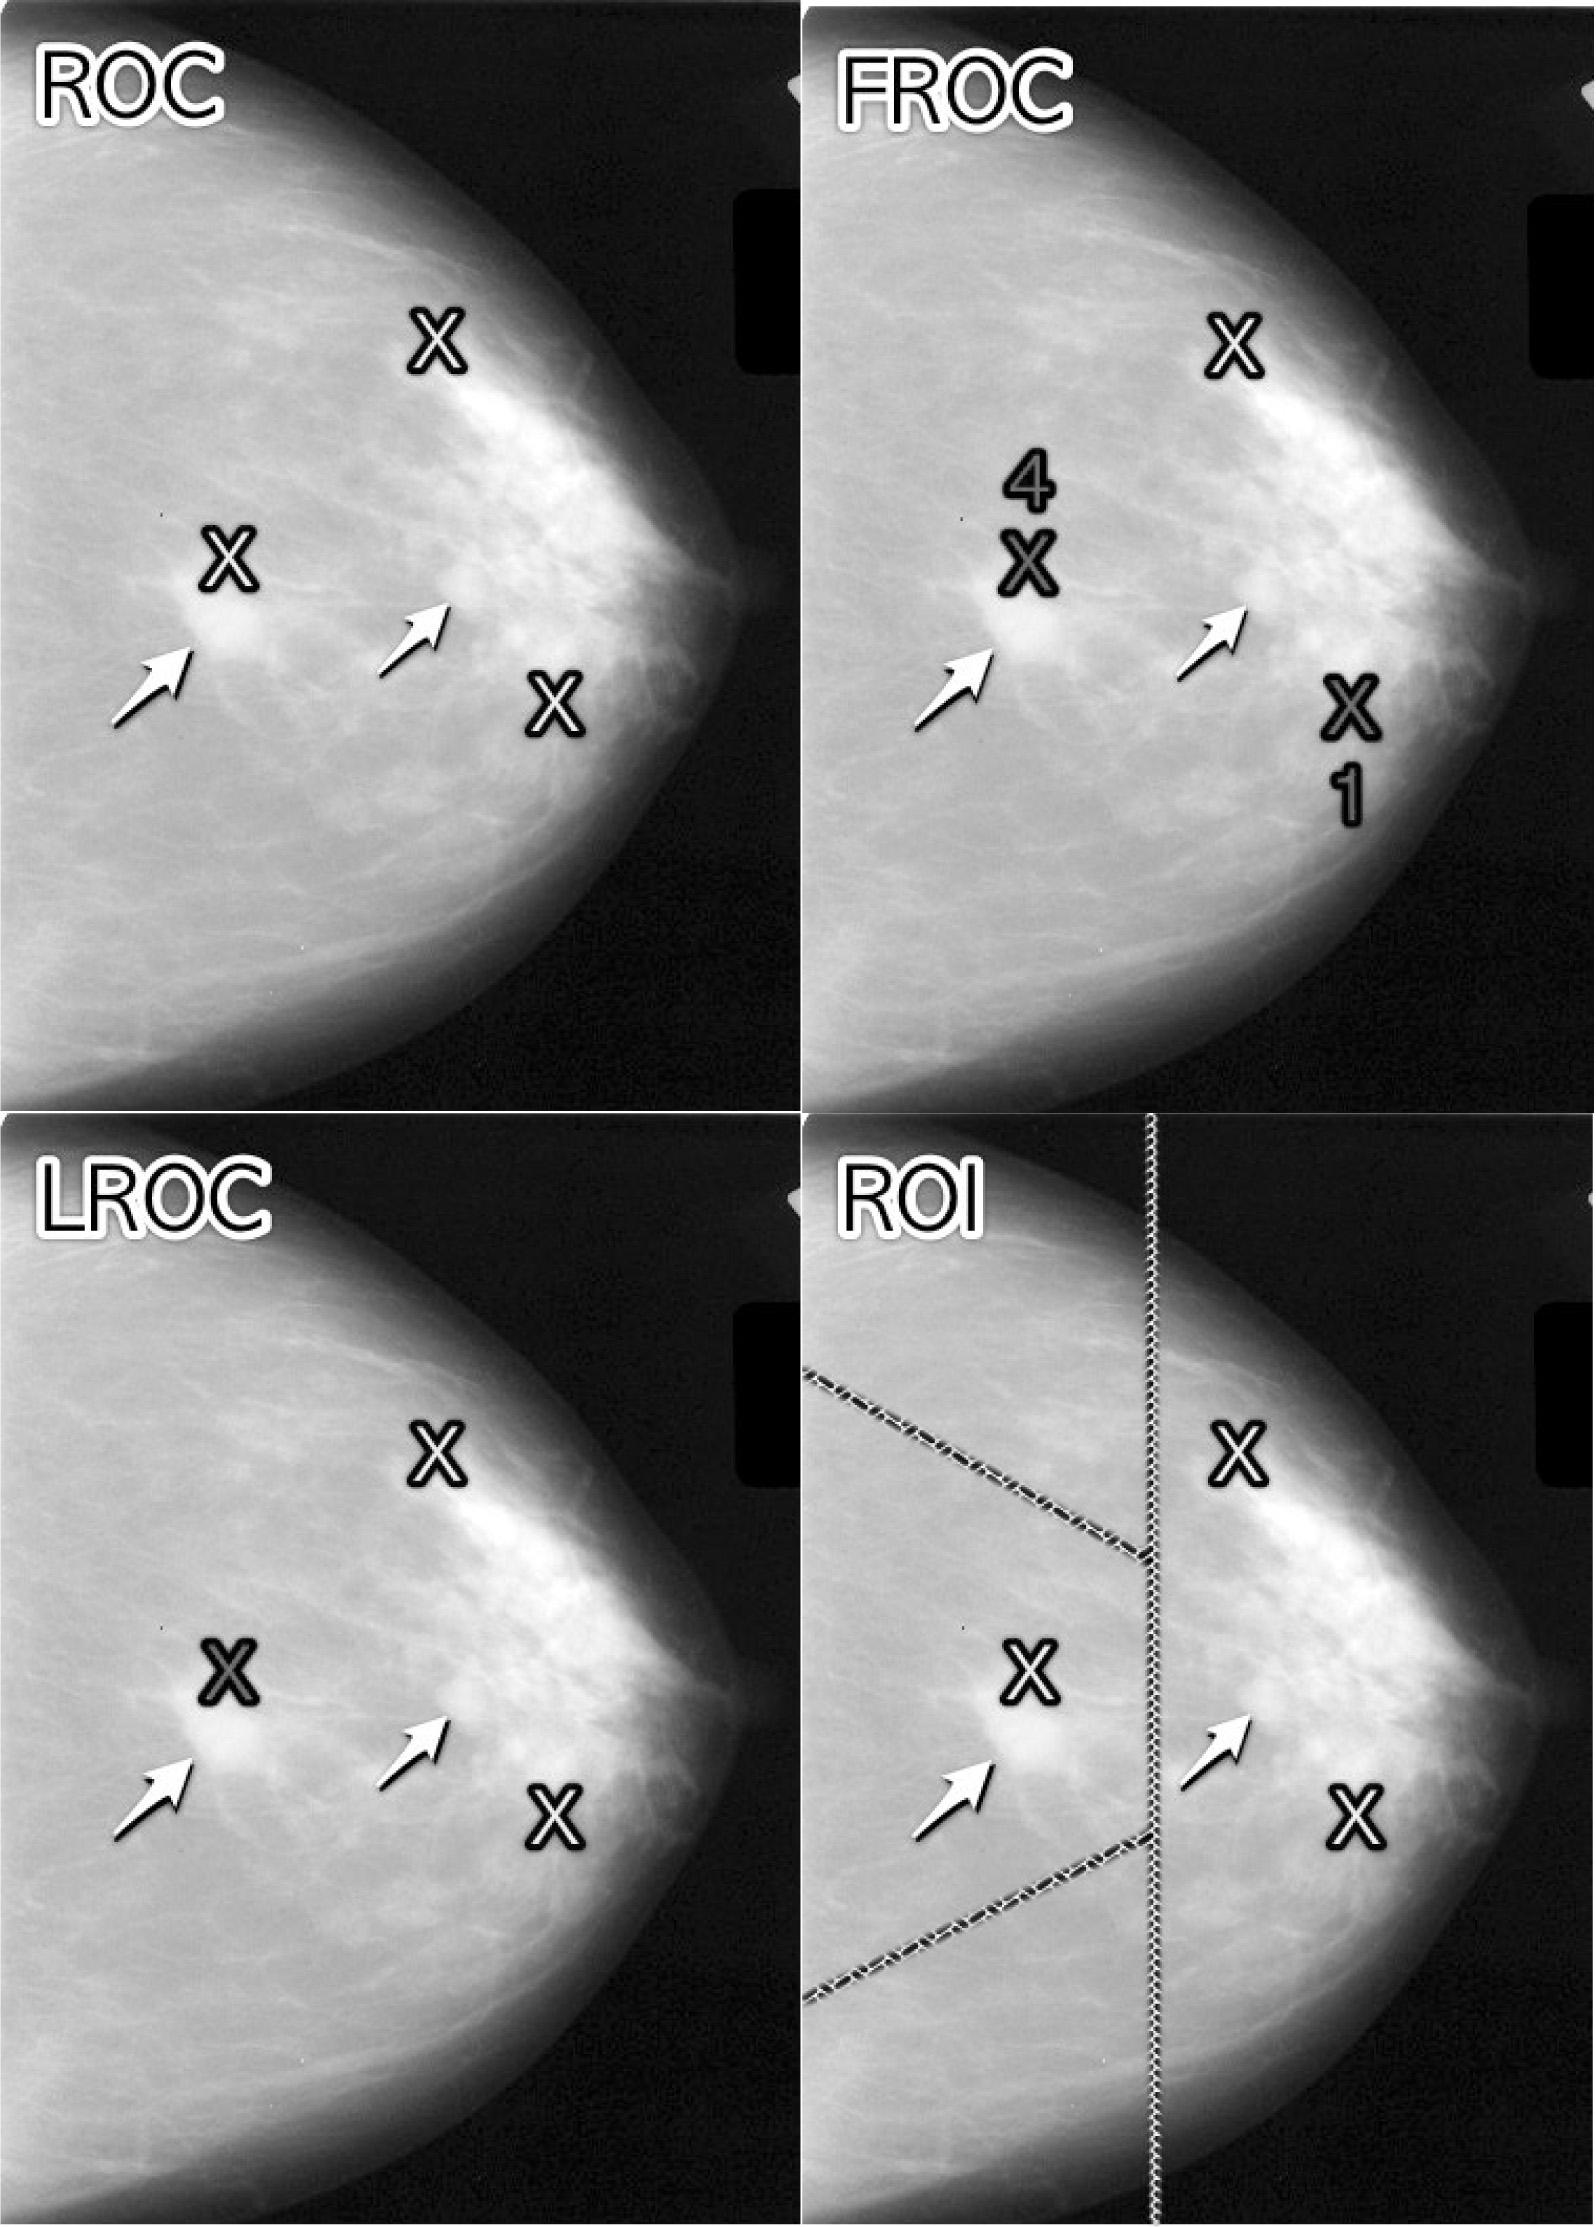
\includegraphics[width=300pt]{images/4Paradigms} 

}

\caption{Observer performance paradigms in use: Upper Left -- ROC, Upper Right -- FROC, Lower Left -- LROC, Lower Right -- ROI}\label{fig:froc-paradigm-4}
\end{figure}

\begin{quote}
In this book \emph{lesion} always refers to a true or real lesion. The term \emph{suspicious region} or \emph{perceived lesion} is reserved for any region that, as far as the observer is concerned, has ``lesion-like'' characteristics. \emph{A lesion is a real entity while a suspicious region is a perceived entity.}
\end{quote}

\begin{itemize}
\item
  In the ROC paradigm, Fig. \ref{fig:froc-paradigm-4} (top-left panel), the radiologist assigns a single rating indicating the confidence level that there is at least one lesion somewhere in the image. Assuming a 1 -- 5 positive directed integer rating scale if the left-most light-shaded cross is a highly suspicious region then the ROC rating might be 5 (highest confidence for presence of disease). There are no dark-shaded crosses on this panel as no marking occurs in the ROC paradigm.
\item
  In the free-response (FROC) paradigm, Fig. \ref{fig:froc-paradigm-4} (top-right panel), the two dark-shaded crosses indicate suspicious regions that were \emph{marked}, and the adjacent numbers are the corresponding ratings. \emph{In this example the two ratings shown apply to two specific suspicious regions, unlike the ROC paradigm where the single rating applies to the whole image.} Assuming the allowed FROC ratings are integers 1 through 4 two marks are shown, one rated FROC-4, which is close to a true lesion, and the other rated FROC-1, which is not close to any true lesion. The third suspicious region, indicated by the light-shaded cross, was not marked, implying its confidence level did not exceed the lowest reporting threshold for a FROC-1 rating. The marked region rated FROC-4 (the highest FROC confidence level) is likely what caused the radiologist to assign the ROC-5 rating to this image in the ROC paradigm panel.
\item
  In the LROC paradigm, Fig. \ref{fig:froc-paradigm-4} (bottom-left panel), the radiologist rates the confidence that there is at least one lesion somewhere in the image (as in the ROC paradigm) and marks the \emph{most suspicious} region in the image. In this example the rating might be LROC-5, the five rating being the same as in the ROC paradigm, and the mark may be the suspicious region rated FROC-4 in the FROC paradigm panel, and, since it is close to a true lesion, in LROC terminology it would be recorded as a \emph{correct localization}. If the mark were not near a lesion it would be recorded as an \emph{incorrect localization}. Only one mark is allowed in this paradigm, and in fact one mark is \emph{required} on every image, even if the observer does not find any suspicious regions to report.
\item
  In the region of interest (ROI) paradigm the researcher segments the image into a number of regions-of-interest (ROIs) and the radiologist rates each ROI for presence of at least one suspicious region within the ROI. The rating is similar to the ROC rating, except it applies to the ROI, not the whole image. Assuming a 1 -- 5 positive directed integer rating scale in Fig. \ref{fig:froc-paradigm-4} (bottom-right panel) there are four ROIs. The ROI at \textasciitilde9 o'clock might be rated ROI-5 as it contains the most suspicious light-shaded cross (the region that was rated FROC-4), the one at \textasciitilde11 o'clock might be rated ROI-1 as it does not contain any light-shaded crosses, the one at \textasciitilde3 o'clock might be rated LROC-2 or LROC-3 (the unmarked light-shaded cross would tend to increase the confidence level) and the one at \textasciitilde7 o'clock might be rated ROI-1\footnote{The ROIs could be clinically driven descriptors of location, such as ``apex of lung'' or ``mediastinum'', and the image does not have to have lines showing the ROIs (which would be distracting to the radiologist). The number of ROIs per image can be at the researcher's discretion and there is no requirement that every case have the same number of ROIs.}.
\end{itemize}

\hypertarget{froc-paradigm-vis-search}{%
\section{Visual search}\label{froc-paradigm-vis-search}}

Any search task has two components: finding something\footnote{while not finding irrelevant stuff, a subtle but important point} and acting on it. Familiar examples of a search tasks are looking for lost car-keys or a milk carton in the refrigerator. Success in a search task is finding the searched for object\footnote{without finding too many extraneous objects}. Acting on it could be driving to work or drinking milk from the carton\footnote{There is expertise associated with any search task. Husbands are notoriously bad at finding the milk carton in the refrigerator (analogy due to Dr.~Elizabeth Krupinski at an SPIE course taught jointly with the author).}.

Likewise, a medical imaging search task has two components: finding lesions and acting on each finding\footnote{``Finding'' is the actual term used by radiologists in their clinical reports}. The latter involves determining if it is sufficiently suspicious for cancer to warrant reporting and further patient follow-up. Such a region is marked and rated for confidence that it is a malignant lesion.

The radiologist does not know a-priori if the patient is diseased and, if diseased, how many lesions may be present. In the breast-screening context, it is known that about 5 out of 1000 patients have cancers, so 99.5\% of the time odds are that the patient has no malignant lesions\footnote{The probability of benign suspicious regions is much higher \citep{Ernster1981Epidemiology}, about 13\% for women aged 40-45.}. Considerably search expertise is needed for the radiologist to mark malignant lesions with high probability \emph{while not generating too many false marks, for doing so degrades success in a search task}. The italicized clause is important - too many marks, one of which might be the real lesion, would slow down the ability of the radiologist to diagnose the patient as each of the false marks would need to be ruled out.

At my former institution (University of Pittsburgh) the radiologists digitally outline and annotate (describe) suspicious region(s) that are found. As one would expect from the low prevalence of breast cancer in the screening context and assuming expert-level radiologist interpretations, about 90\% of breast cases do not generate any marks. About 10\% of cases generate one or more marks and are recalled for further comprehensive imaging (termed diagnostic workup). Of marked cases about 90\% generate one mark, about 10\% generate 2 marks, and a rare case generates 3 or more marks (Dr.~David Gur, private communication, ca. 2015).

Conceptually, a mammography report consists of the locations of regions that exceed the threshold and the corresponding levels of suspicion, reported as a Breast Imaging Reporting and Data System (BIRADS) rating. The BIRADS rating is actually assigned after the diagnostic workup following a screening BIRADS-0 rating. The screening rating itself is binary: BIRADS-0 for recall (the patient is recalled for a diagnostic workup to determine the final BIRADS rating) or BIRADS-1 for normal or no abnormality detected (the patient comes back about a year later for the next screening appointment).

\begin{quote}
The FROC paradigm in medical imaging is a visual search task.
\end{quote}

\hypertarget{froc-paradigm-scoring-the-data}{%
\subsection{Proximity criterion and scoring the data}\label{froc-paradigm-scoring-the-data}}

In the first quasi-clinical application of the FROC paradigm \citep{Chakraborty1986DigitalVsConv} the marks and ratings were indicated by a grease pencil on an acrylic overlay aligned, in a reproducible way, to the CRT displayed chest image of an anthropomorphic chest phantom with superposed simulated lesions. Credit for a correct detection and localization, termed a lesion-localization or LL-event\footnote{The proper terminology for this paradigm has evolved. Older publications and some newer ones refer to this as a true positive (TP) event, thereby confusing a ROC related term that does not involve search with one that does.}, was given only if a mark was sufficiently close (as per proximity criterion, see below) to an actual diseased region; otherwise, the observer's mark was scored as a non-lesion localization or NL-event.

\begin{quote}
The use of ROC terminology such as true positives or false positives to describe FROC data is not conducive to clarity and is strongly discouraged.
\end{quote}

Definitions:

\begin{quote}
\begin{itemize}
\tightlist
\item
  NL = non-lesion localization, i.e., a mark that is not close to any lesion
\item
  LL = lesion localization, i.e., a mark that is close to a lesion
\end{itemize}
\end{quote}

One adopts an acceptance radius (for spherical lesions) or \emph{proximity criterion} (the more general case). What constitutes ``close enough'' is a clinical decision the answer to which depends on the application. It is not necessary for two radiologists to point to the same pixel in order for them to agree that they are seeing the same suspicious region. Likewise, two physicians -- e.g., the radiologist finding the lesion on an x-ray and the surgeon responsible for resecting it -- do not have to agree on the exact center of a lesion in order to appropriately assess and treat it. More often than not, ``clinical common sense'' can be used to determine if a mark actually localized the lesion. When in doubt, the researcher should ask an independent radiologist (i.e., not one used in the observer study) how to score ambiguous marks. A rigid definition of the proximity criterion should not be used.

For roughly spherical nodules a simple rule can be used. If a circular lesion is 10 mm in diameter, one can use the ``touching-coins'' analogy to determine the criterion for a mark to be classified as lesion localization. Each coin is 10 mm in diameter so if they touch their centers are separated by 10 mm and the rule is to classify any mark within 10 mm of an actual lesion center as a LL mark, and if the separation is greater the mark is classified as a NL mark. A recent paper \citep{Dobbins2016MultiInstitutional} using FROC analysis gives more details on appropriate proximity criteria in the clinical context in a study involving both volumetric (CT) and 2D chest images.\footnote{Generally the proximity criterion is more stringent for smaller lesions than for larger one. However, for very small lesions allowance is made so that the criterion does not penalize the radiologist for normal marking ``jitter''. For 3D images the proximity criteria is different in the x-y plane vs.~the slice thickness axis.}

\hypertarget{multiple-marks-in-the-same-vicinity}{%
\subsection{Multiple marks in the same vicinity}\label{multiple-marks-in-the-same-vicinity}}

Multiple marks near the same vicinity are rarely encountered with radiologists, especially if the perceived lesion is mass-like. \footnote{The exception would be if the perceived lesions were speck-like objects in a mammogram, and even here radiologists tend to broadly outline the region containing perceived specks -- they do not mark individual specks with great precision.} However, algorithmic readers, such as computer aided detection (CAD) algorithms, tend to find multiple regions in the same area. Algorithm designers generally incorporate a clustering step to reduce overlapping regions to a single region and assign the highest rating to it (i.e., the rating of the highest rated mark, not the rating of the closest mark. \footnote{The reason for using the highest rating is that this gives full and deserved credit for the localization. Other marks in the same vicinity with lower ratings need to be discarded from the analysis; specifically, they should not be classified as NLs, because each mark has successfully located the true lesion to within the clinically acceptable criterion, i.e., any one of them is a good decision because it would result in a patient recall and point further diagnostics to the true location.}

\hypertarget{historical-context}{%
\subsection{Historical context}\label{historical-context}}

The term ``free-response'' was coined by \citep{RN897} to describe a task involving the detection of brief audio tone(s) against a background of white-noise (white-noise is what one hears if an FM tuner is set to an unused frequency). The tone(s) could occur at any instant within an active listening interval, defined by an indicator light bulb that is turned on. The listener's task was to respond by pressing a button at the specific instant(s) when a tone(s) was perceived (heard). The listener was uncertain how many true tones could occur in an active listening interval and when they might occur. Therefore, the number of responses (button presses) per active interval was a priori unpredictable: it could be zero, one or more. The Egan et al study did not require the listener to rate each button press, but apart from this difference and with two-dimensional images replacing the listening intervals, the acoustic signal detection study is similar to medical imaging search tasks.

\hypertarget{froc-paradigm-froc-plot}{%
\section{The FROC plot}\label{froc-paradigm-froc-plot}}

The free-response receiver operating characteristic (FROC) plot was introduced \citep{RN2104} as a way of visualizing performance in the free-response auditory tone detection task.

In the medical imaging context, assuming the mark rating pairs have been classified as NLs (non-lesion localizations) or LLs (lesion localizations):

\begin{itemize}
\item
  Non-lesion localization fraction (NLF) is defined as the total number of NLs rated at or above a threshold rating divided by the total number of cases.
\item
  Lesion localization fraction (LLF) is defined as the total number of LLs rated at or above the same threshold rating divided by the total number of lesions.
\item
  The FROC plot is defined as that of LLF (ordinate) vs.~NLF as the threshold is varied.
\item
  The upper-right-most operating point is termed the \emph{observed end-point} and its coordinates are denoted \((\text{NLF}_{\text{max}}, \text{LLF}_{\text{max}})\).
\end{itemize}

The rating can be any real number, as long as higher values are associated with higher confidence levels.

If \emph{integer ratings} are used then in a four-rating FROC study at most 4 FROC operating points will result: one corresponding to marks rated 4s; another corresponding to marks rated 4s or 3s; another to the 4s, 3s, or 2s; and finally the 4s, 3s, 2s, or 1s. An R-rating study yields at most R operating points \footnote{I have seen publications that describe a data collection process where the ``1'' rating is used to mean, in effect, that the observer sees nothing to report in the image, i.e., to mean ``let's move on to the next image''. This amounts to wasting a confidence level. The user interface should present an explicit ``next-image'' option and reserve the ``1'' rating to mean the lowest reportable confidence level.}.

If \emph{continuous ratings} are used, the procedure is to start with a very high threshold so that none of the ratings exceed the threshold and then to gradually lower the threshold. Every time the threshold crosses the rating of a mark, or possibly multiple marks, the total count of LLs and NLs exceeding the threshold is divided by the appropriate denominators yielding the `'raw'' FROC plot. For example, when an LL rating just exceeds the threshold, the operating point jumps up by 1/(total number of lesions), and if two LLs simultaneously just exceed the threshold the operating point jumps up by 2/(total number of lesions). If an NL rating just exceeds the threshold, the operating point jumps to the right by 1/(total number of cases). If an LL rating and a NL rating simultaneously just exceed the threshold, the operating point moves diagonally, up by 1/(total number of lesions) and to the right by 1/(total number of cases). The reader should get the general idea by now and recognize that the cumulating procedure is very similar to the manner in which ROC operating points were calculated, the only differences being in the quantities being cumulated and the relevant denominators.

Empirical plot:

\begin{quote}
A plot is termed \emph{empirical} if is based on the observed operating points only; one simply connects adjacent operating points (including the origin) with straight lines.
\end{quote}

Chapter \ref{empirical} describes the empirical FROC and other possible operating characteristics in more detail.

\hypertarget{froc-paradigm-plot-illustration}{%
\subsection{Illustration with a dataset}\label{froc-paradigm-plot-illustration}}

The following code uses \texttt{dataset04} \citep{zanca2009evaluation} in \texttt{RJafroc} to illustrate an empirical FROC plot. The dataset has 5-treatments and 4 readers, so in principle one can generate 20 plots. In this example I have selected treatment 1 and reader 1 to produce the plot. The reader should experiment by running, for example \texttt{PlotEmpiricalOperatingCharacteristics(dataset04,\ trts\ =\ 2,\ rdrs\ =\ 1,\ opChType\ =\ "FROC")\$Plot}, i.e., with different treatments and readers specified.

\begin{Shaded}
\begin{Highlighting}[]
\NormalTok{ret }\OtherTok{\textless{}{-}} \FunctionTok{PlotEmpiricalOperatingCharacteristics}\NormalTok{(}
\NormalTok{  dataset04, }
  \AttributeTok{trts =} \DecValTok{1}\NormalTok{, }\AttributeTok{rdrs =} \DecValTok{1}\NormalTok{, }\AttributeTok{opChType =} \StringTok{"FROC"}\NormalTok{)}
\FunctionTok{print}\NormalTok{(ret}\SpecialCharTok{$}\NormalTok{Plot)}
\end{Highlighting}
\end{Shaded}

\includegraphics{02-froc_files/figure-latex/unnamed-chunk-1-1.pdf}

The study in question was a 5 rating FROC study. The lowest non-trivial point (i.e., not counting the trivial origin which is common to all FROC plots) corresponds to the marks rated 5, the next higher one corresponds to marks rated 4 or 5, etc. FROC plots may vary widely in shape but they share the common characteristic that the operating point cannot move downward or to the left as one cumulates lower confidence level marks (i.e., it can only move upward and to the right; the plot can flatten out or it can end at a finite value of NLF).

The plot shown above is termed an \emph{empirical plot} as it consists of the empirical (observed) operating points connected by straight line segments.

\hypertarget{froc-paradigm-solar-analogy}{%
\section{The ``solar'' analogy}\label{froc-paradigm-solar-analogy}}

Consider the sun, regarded as a ``lesion'' to be detected, with two daily observations spaced 12 hours apart, so that at least one observation period is bound to have the sun in the sky. Furthermore assume the observer knows his GPS coordinates and has a watch that gives accurate local time, from which an accurate location of the sun can be deduced. Assuming clear skies and no obstructions to the view, the sun will always be correctly located and no rational observer will ever generate a non-lesion localization or NL, i.e., no region of the sky will be erroneously ``marked'' as being the sun.

FROC curve implications of this analogy are:

\begin{itemize}
\tightlist
\item
  Each 24-hour day corresponds to two ``trials'' in the \citep{RN897} sense, or two cases -- one diseased and one non-diseased -- in the medical imaging context.
\item
  The denominator for calculating LLF is the total number of AM days, and the denominator for calculating NLF is twice the total number of 24-hour days.
\item
  Most important, \(\text{LLF}_{\text{max}} = 1\) and \(\text{NLF}_{\text{max}} = 0\).
\end{itemize}

In fact, even when the sun is not directly visible due to heavy cloud cover, since the actual location of the sun can be deduced from the local time and GPS coordinates, the rational observer will still ``mark'' the correct location of the sun and not make any false sun localizations. Consequently, even in this example \(\text{LLF}_{\text{max}} = 1\) and \(\text{NLF}_{\text{max}} = 0\).

The conclusion is that in a task where a target is known to be present in the field of view and its location is known, the observer will always achieve \(\text{LLF}_{\text{max}} = 1\) and \(\text{NLF}_{\text{max}} = 0\). Why are LLF and NLF subscripted ``max''? By randomly choosing to not mark the position of the sun even though it is visible, for example, using a coin toss to decide whether or not to mark the sun, the observer can ``walk down'' the y-axis of the FROC plot, eventually reaching \(LLF = 0\) and \(NLF = 0\). The reason for allowing the observer to ``walk down'' the vertical is simply to demonstrate that a continuous FROC curve from the origin to (0,1) can, in fact, be realized.

Now consider a fictitious otherwise earth-like planet where the sun can be at random positions rendering GPS coordinates and the local time useless. All one knows is that the sun is somewhere in the upper or lower hemispheres subtended by the sky. If there are no clouds and consequently one can see the sun clearly during daytime, a rational observer would still correctly locate the sun while not marking the sky with any incorrect sightings, so \(\text{LLF}_{\text{max}} = 1\) and \(\text{NLF}_{\text{max}} = 0\). This is because, in spite of the fact that the expected location is unknown, the high contrast sun is enough the trigger the peripheral vision system, so that even if the observer did not start out looking in the correct direction, peripheral vision will guide the observer's gaze to the correct location.

The implication of this is that a fundamentally different mechanism from that considered in conventional observer performance methodology, namely \emph{search}, is at work.

\begin{quote}
Search describes the process of \emph{finding} lesions while \emph{not finding} non-lesions and search performance is the ability to find all lesions while minimizing finding non-lesions.
\end{quote}

Think of the eye as two cameras: a low-resolution camera (peripheral vision) with a wide field-of-view plus a high-resolution camera (foveal vision) with a narrow field-of-view If one were limited to viewing with the high-resolution camera one would spend so much time steering the high-resolution narrow field-of-view camera from spot-to-spot that one would have a hard time finding the desired stellar object. Having a single high-resolution narrow field of view vision would also have negative evolutionary consequences as one would spend so much time scanning and processing the surroundings with the narrow field of view vision that one would miss dangers or opportunities. Nature has equipped us with essentially two cameras; the first low-resolution camera is able to ``digest'' large areas of the surround and process it rapidly so that if danger (or opportunity) is sensed, then the eye-brain system rapidly steers the second high-resolution camera to the location of the danger (or opportunity). This is Nature's way of optimally using the eye-brain system. For a similar reason astronomical telescopes come with a wide field of view lower magnification ``spotter scope''.

When cloud cover completely blocks the fictitious random-position sun there is no stimulus to trigger the peripheral vision system to guide the fovea to the correct location. The observer is reduced to guessing and is led to different conclusions depending upon the benefits and costs involved. If, for example, the guessing observer earns a dollar for each LL and is fined a dollar for each NL, then the observer will likely not make any marks as the chance of winning a dollar is much smaller than losing many dollars. For this observer \(\text{LLF}_{\text{max}} = 0\) and \(\text{NLF}_{\text{max}} = 0\), and the operating point is ``stuck'' at the origin. If, on the other hand, the observer is told every LL is worth a dollar and there is no penalty to NLs, then with no risk of losing the observer will ``fill up'' the sky with false marks.

The analogy is not restricted to the sun, which one might argue is an almost infinite SNR object and therefore atypical. Consider finding stars or planets. In clear skies, if one knows the constellations, one can still locate bright stars and planets like Venus or Jupiter. With less bright stars and / or obscuring clouds, there will be false-sightings and the FROC plot could approach a flat horizontal line at ordinate equal to zero, but the observer will not fill up the sky with false sightings of a desired star.

False sightings of objects in astronomy do occur. Finding a new astronomical object is a search task, where, as always, one can have two outcomes, correct localization (LL) or incorrect localizations (NLs). At the time of writing there is a hunt for a new planet, possibly a gas giant , that is much further than even the newly demoted Pluto.

\hypertarget{froc-paradigm-discussion}{%
\section{Discussion}\label{froc-paradigm-discussion}}

The FROC paradigm is often misunderstood. Some of this has to do with loose terminology and some to misconceptions regarding the meaning of search, the paradigm and the FROC curve. These are summarized below (I could cite the offending examples but no useful purpose will be served by my doing so):

\begin{itemize}
\tightlist
\item
  Loose terminology:

  \begin{itemize}
  \tightlist
  \item
    Using the term ``lesion-specific'' to describe location-specific paradigms.
  \item
    Using the term ``lesion'' when one means a ``suspicious region'' that may or may not be a true lesion.
  \item
    Using ROC paradigm terms, such as true positive and false positive, that apply to the whole case, to describe location-specific terms such as lesion and non-lesion localizations, that apply to regions of the image. This is very common.
  \item
    Using the FROC-1 rating to mean in effect ``I see no signs of disease in this image'' when in fact it should be used as the lowest level of a reportable suspicious region. The former usage amounts to wasting a confidence level.
  \end{itemize}
\item
  Misconception:

  \begin{itemize}
  \tightlist
  \item
    A fundamental misunderstanding of search performance is embodied in the statement \emph{``CAD is perfect at search because it looks at everything''}.
  \item
    Showing FROC curves as reaching the unit ordinate as this is the exception rather than the rule.
  \item
    Believing that FROC curves extend to very large values (potentially infinite) along the abscissa and all the observer has to do to access this region is to lower their reporting threshold.
  \end{itemize}
\end{itemize}

The FROC plot is historically the first proposed way of visually summarizing FROC data. The next chapter deals with all empirical operating characteristics that can be defined from an FROC dataset that have evolved over the years.

\hypertarget{empirical}{%
\chapter{Empirical plots from FROC data}\label{empirical}}

\hypertarget{empirical-how-much-finished}{%
\section{How much finished}\label{empirical-how-much-finished}}

100\%

\hypertarget{empirical-intro}{%
\section{Introduction}\label{empirical-intro}}

FROC data consists of mark-rating pairs. A distinction is made between \emph{latent} marks (suspicious regions perceived by the visual system but not necessarily marked) and \emph{actual} marks. A key table (used in later chapters) summarizing FROC notation is introduced which allows unambiguous description of the data.

Empirical plots refer to those generated directly from the data. Empirical operating characteristics (empirical plots) introduced in this chapter are the FROC, the (inferred) ROC, the alternative FROC (AFROC), the weighted AFROC (wAFROC), the AFROC1, wAFROC1. Formulae for x and y coordinates of each plot are given in terms of the underlying mark-rating FROC data.

Plots are \emph{visual} depictions of performance. Scalar measures derived from plots can serve as \emph{quantitative} measures of performance. Empirical area under curve (AUC) measures associated with all plots are illustrated with a small FROC dataset. Except for the FROC plot all of the other plots include a straight line extension from the uppermost observed operating point to (1,1).

If one ignores localization information and simply considers the highest rating on each case as representing its ROC rating, one can define the empirical ROC plot and associated area measure ROC-AUC from FROC data. Since ROC-AUC is a fundamental measure of classification accuracy between non-diseased and diseased cases any other proposed area measure that does not ignore location information should, if it is to be useful, correlate with ROC-AUC. These correlations are explored using the small dataset and it is shown that FROC-AUC is a poor measure of performance. While ways of circumventing FROC-AUC have been proposed and have been used by some investigators none are satisfactory and the claim of this book is that \textbf{the FROC should never be used to quantify performance}. The basic reason is simple: unlike all of the other plots defined in this chapter the FROC plot is not constrained to lie within the unit square and the area under a straight line extension to (1,1) is meaningless.

Some of the other empirical plots and AUCs are less familiar as compared to the well-known ROC plots and ROC-AUC. As an aid to understanding them I have included numerical (``hand'') calculations of the empirical plots and AUCs for the small dataset. The calculations also illustrate the advantage of using \emph{weighted} versions implemented in some of the empirical plots (lesion weights are a way of allowing one to model the clinical importance (i.e., morbidity/mortality) associated with different type of lesions present in a clinical dataset; a weighted plot assures that each case gets the same importance in determining AUC regardless of the number of lesions in it).

Computing the AUCs from plots can be tedious at best; computational formulae are needed which would allow any of the AUCs to be calculated directly from the FROC ratings. Appendix 1 proves a formula for the wAFROC-AUC, Appendix 2 provides a physical interpretation of the area under the straight line extension for this plot. Appendix 3 summarizes, without proofs, the computational formulae for AUCs for all plots introduced in this chapter.

\hypertarget{empirical-mark-rating-pairs}{%
\section{FROC data and notation}\label{empirical-mark-rating-pairs}}

\hypertarget{lls-vs.-nls}{%
\subsection{LLs vs.~NLs}\label{lls-vs.-nls}}

Each mark indicates the location of a region suspicious enough to warrant reporting and the rating is the associated confidence level. A mark is recorded as a \emph{lesion localization} (LL) if it is sufficiently close to a true lesion and otherwise it is recorded as a \emph{non-lesion localization} (NL).

In an FROC study the number of marks on a case is an a-priori unknown non-negative random integer. It is incorrect and naive to estimate it by dividing the anatomically-relevant image area by the lesion area because not all regions of the image are equally likely to have lesions, lesions do not have the same size, and perhaps most important, radiologists don't assign equal attention units to all areas of the image \footnote{Currently the best insight into the numbers and locations of marks per case is obtained from eye-tracking studies \citep{duchowski2017eye}, but the information is incomplete as eye-tracking studies can only measure \emph{foveal} gaze and not lesions found by \emph{peripheral} vision. Moreover, such studies are near impossible to conduct in a clinical setting (at least with the eye-tracking apparatus that I am familiar with).}.

\hypertarget{latent-vs.-actual-marks}{%
\subsection{Latent vs.~actual marks}\label{latent-vs.-actual-marks}}

To distinguish between suspicious regions that were considered for marking but not necessarily marked and regions that were actually marked, it is necessary to introduce the distinction between \emph{latent} marks and \emph{actual} marks.

\begin{itemize}
\tightlist
\item
  A \emph{latent} mark is defined as a suspicious region, regardless of whether or not it was marked. A latent mark becomes an \emph{actual} mark if it is marked.
\item
  A latent mark is a latent LL if it is close to a true lesion and otherwise it is a latent NL.
\item
  A non-diseased case can only have latent NLs. A diseased case can have latent NLs and latent LLs.
\item
  If marked a latent NL is recorded as an actual NL.
\item
  If not marked a latent NL is an \emph{unobservable event}. This is an important point.
\item
  In contrast unmarked lesions are observable events -- one knows (trivially) which lesions were not marked.
\end{itemize}

\hypertarget{z-samples-vs.-ratings}{%
\subsection{z-samples vs.~ratings}\label{z-samples-vs.-ratings}}

z-samples are conceptual quantities that can range from \(-\infty\) to \(+\infty\). Ratings are observed values typically collected as integers but any ordered set of values will do where larger values correspond to greater suspicion for disease. The conversion from z-samples to ratings is accomplished by adopting a binning rule.

\hypertarget{binning-rule}{%
\subsection{Binning rule}\label{binning-rule}}

Recall that ROC data modeling requires the existence of a \emph{case-dependent} decision variable, or z-sample \(z\), and case-independent decision thresholds \(\zeta_r\), where \(r = 0, 1, ..., R_{ROC}-1\), where \(R_{ROC}\) is the number of ROC study bins \footnote{The subscript is used to make explicit the paradigm used as otherwise it leads to confusion.} and a \emph{binning rule} that if \(\zeta_r \leq z < \zeta_{r+1}\) the case is rated \(r + 1\). Dummy cutoffs are defined as \(\zeta_0 = -\infty\) and \(\zeta_{R_{ROC}} = \infty\). The z-sample applies to the whole case. To summarize:

\begin{equation}
\left.
\begin{aligned}  
\text{if} \left (\zeta_r \le z < \zeta_{r+1}  \right )\Rightarrow \text {rating} = r+1\\
r = 0, 1, ..., R_{ROC}-1\\
\zeta_0 = -\infty\\
\zeta_{R_{ROC}} = \infty\\
\end{aligned}
\right \}
\label{eq:binning-rule-roc}
\end{equation}

Analogously, FROC data modeling requires the existence of a \emph{case and location dependent} z-sample for each latent mark and \emph{case and location independent} reporting thresholds \(\zeta_r\), where \(r = 1, ..., R_{FROC}\) and \(R_{FROC}\) is the number of FROC study bins, and the binning rule that a latent mark is marked and rated \(r\) if \(\zeta_r \leq z < \zeta_{r+1}\). Dummy cutoffs are defined as \(\zeta_0 = -\infty\) and \(\zeta_{R_{FROC}+1} = \infty\). For the same numbers of non-dummy cutoffs, the number of FROC bins is one less than the number of ROC bins. For example, 4 non-dummy cutoffs \(\zeta_1, \zeta_2, \zeta_3, \zeta_4\) can correspond to a 5-rating ROC study or to a 4-rating FROC study. To summarize:

\begin{equation}
\left.
\begin{aligned}  
\text{if} \left (\zeta_r \le z < \zeta_{r+1}  \right )\Rightarrow \text {rating} = r\\
r = 1, 2, ..., R_{FROC}\\
\zeta_0 = -\infty\\
\zeta_{R_{FROC}+1} = \infty\\
\end{aligned}
\right \}
\label{eq:binning-rule-froc}
\end{equation}

\hypertarget{empirical-notation}{%
\subsection{Notation}\label{empirical-notation}}

\emph{Clear notation is vital to understanding this paradigm.} The notation needs to account for case and location dependencies of ratings and the distinction between case-level and location-level ground truths. \emph{The notation also has to account for cases with no marks.}

FROC notation is summarized in Table \ref{tab:empirical-notation} in which ``marks'' refer to ``latent marks''. The first column is the row number, the second column has the symbol(s), and the third column has the meaning(s) of the symbol(s).

\begin{table}

\caption{\label{tab:empirical-notation}FROC notation; all marks refer to latent marks.}
\centering
\begin{tabular}[t]{l|l|l}
\hline
Row & Symbol & Meaning\\
\hline
1 & $t$ & Case-level truth: 1 non-diseased, 2 diseased case\\
\hline
2 & $K_t$ & Number of cases with case-level truth $t$\\
\hline
3 & $k_t t$ & Case $k_t$ in case-level truth $t$\\
\hline
4 & $s$ & Location-level truth: 1 for NL and 2 for LL\\
\hline
5 & $l_s s$ & Mark $l_s$ in location-level truth $s$\\
\hline
6 & $N_{k_t t}$ & Number of NLs in case $k_t t$\\
\hline
7 & $L_{k_2 2}$ & Number of lesions in case $k_2 2$\\
\hline
8 & $z_{k_t t l_1 1}$ & $z$-sample for case $k_t t$ and NL mark $l_1 1$\\
\hline
9 & $z_{k_2 2 l_2 2}$ & $z$-sample for case $k_2 2$ and LL mark $l_2 2$\\
\hline
10 & $r_{k_t t l_s s}$ & rating for case $k_t t$ and LL/NL mark $l_s s$\\
\hline
11 & $R_{FROC}$ & Number of FROC bins\\
\hline
12 & $\zeta_1$ & Lowest non-dummy reporting threshold\\
\hline
13 & $\zeta_r$ & $r$ = 2, 3, ..., non-dummy reporting thresholds\\
\hline
14 & $\zeta_0, \zeta_{R_{FROC}+1}$ & Dummy thresholds, negative and positive infinity\\
\hline
15 & $W_{k_2 l_2}$ & Weight of lesion $l_2 2$ in case $k_2 2$, explained later\\
\hline
16 & $L_{max}$ & Maximum number of lesions per case in dataset\\
\hline
17 & $L_T$ & Total number of lesions in dataset\\
\hline
\end{tabular}
\end{table}

\hypertarget{comments}{%
\subsection{Comments}\label{comments}}

\begin{itemize}
\item
  Row 1: The case-truth index \(t\) refers to the case (or patient), with \(t = 1\) for non-diseased and \(t = 2\) for diseased cases. As a useful mnemonic, \(t\) is for \emph{truth}.
\item
  Row 2: \(K_t\) is the number of cases with truth state \(t\); specifically, \(K_1\) is the number of non-diseased cases and \(K_2\) the number of diseased cases.
\item
  Row 3: Two indices \(k_t t\) are needed to select case \(k_t\) in truth state \(t\). As a useful mnemonic, \(k\) is for \emph{case}.
\item
  Row 4: \(s\) location-level truth state: 1 for non-diseased region (NL) and 2 for lesion (LL).
\item
  Row 5: Similar to row 3, two indices \(l_s s\) are needed to select latent mark \(l_s\) in location-level truth state \(s\). As a useful mnemonic, \(l\) is for \emph{location}.
\item
  Row 6: \(N_{k_t t}\) is the total number of latent NL marks in case \(k_t t\). Latent NL marks are possible on non-diseased and diseased cases (i.e., both values of \(t\) are allowed).
\item
  Row 7: \(L_{k_2 2}\) is the number of lesions in diseased case \(k_2 2\).
\item
  Row 8: The z-sample for case \(k_t t\) and NL mark \(l_1 1\) is denoted \(z_{k_t t l_1 1}\). The range of a z-sample is \(-\infty < z_{k_t t l_1 1} < \infty\), provided \(l_1 \neq \varnothing\); otherwise, it is an unobservable event.
\item
  Row 9: The z-sample of a latent LL is \(z_{k_2 2 l_2 2}\). Unmarked lesions are observable events assigned negative infinity ratings (the null-set notation is unnecessary).
\item
  Row 10: The rating of a mark is \(r_{k_2 2 l_2 2}\). Unmarked NLs are unobservable events. Unmarked lesions are assigned negative infinity ratings.
\item
  Row 11: \(R_{FROC}\) is the number of bins in the FROC study.
\item
  Rows 12, 13 and 14: The cutoffs in the FROC study. The lowest threshold is \(\zeta_1\). The other non-dummy thresholds are \(\zeta_r\) where \(r=2,3,...,R_{FROC}\). The dummy thresholds are \(\zeta_0 = -\infty\) and \(\zeta_{R_{FROC}+1} = \infty\).
\item
  Row 15: \(W_{k_2 l_2}\) is the weight (i.e., clinical importance) of lesion \(l_2 2\) in diseased case \(k_2 2\). The weights of lesions in a case sum to unity: \(\sum_{l_2 = 1}^{L_{k_2 2}}W_{k_2 l_2} = 1\).
\item
  Row 16: \(L_{max}\) is the maximum number of lesions per case in the dataset.
\item
  Row 17: \(L_T\) is the total number of lesions in the dataset.
\end{itemize}

\hypertarget{empirical-indexing-marks}{%
\subsection{A conceptual and notatonal issue}\label{empirical-indexing-marks}}

An aspect of FROC data, \emph{that there could be cases with no NL marks, no matter how low the reporting threshold}, has created problems both from conceptual and notational viewpoints.

Taking the conceptual issue first, my thinking (prior to 2004) was that as the reporting threshold \(\zeta_1\) is lowered, the number of NL marks per case increases almost indefinitely. I visualized this process as each case ``filling up'' with NL marks \footnote{I expected the number of NL marks per image to be limited only by the ratio of image size to lesion size, i.e., larger values for smaller lesions.}. In fact the first model of FROC data \citep{chakraborty1989maximum} predicts that as the reporting threshold is lowered to \(\zeta_1 = -\infty\), the number of NL marks per case approaches \(\infty\). However, actual FROC datasets do not agree with this thinking. This is one reason I introduced the radiological search model (RSM) \citep{chakraborty2006search}. I will have more to say about this in Chapter \ref{rsm}, but for now I state one assumption of the RSM: the number of latent NL marks is a Poisson distributed random integer with a finite value for the mean parameter of the distribution. This means that the actual number of latent NL marks per case can be 0, 1, 2, .., whose average (over all cases) is a finite number. It is highly unlikely that any case will have an infinite number of NLs.

With this background, let us return to the conceptual issue: why does the observer not keep ``filling-up'' the image with NL marks? The answer is that \emph{the observer can only mark regions that have a non-zero chance of being a lesion}. For example, if the actual number of latent NLs on a particular case is 2, then, as the reporting threshold is lowered, the observer will make at most two NL marks. Having exhausted these two regions the observer will not mark any more regions because there are no more regions to be marked - \emph{all other regions in the image have, in the perception of the observer, zero chance of being a lesion}.

The notational issue is how to handle cases with no latent NL marks. Basically it involves restricting summations over cases to those cases which have at least one latent NL mark, i.e., \(N_{k_t t} > 0\), as in the following:

\begin{itemize}
\item
  \(l_1 = \{1, 2, ..., N_{k_t t}\}\) indexes latent NL marks, provided the case has at least one latent NL mark; otherwise \(N_{k_t t} = 0\) and \(l_1 = \varnothing\), the null set. The possible values of \(l_1\) are \(l_1 = \left \{ \varnothing \right \}\oplus \left \{ 1,2,...N_{k_t t} \right \}\). The null set applies when the case has no latent NL marks and \(\oplus\) is the ``exclusive-or'' symbol (``exclusive-or'' is used in the English sense: ``one or the other, but not neither nor both'').
\item
  \(l_2 = \left \{ 1,2,...,L_{k_2 2} \right \}\) indexes latent LL marks. Unmarked LLs are assigned negative infinity ratings as these are observable events. The null set notation is not needed because for every diseased case \(L_{k_2 2} > 0\).
\end{itemize}

\hypertarget{empirical-froc-plot-1}{%
\section{The FROC plot}\label{empirical-froc-plot-1}}

Definitions:

\begin{quote}
\begin{itemize}
\tightlist
\item
  \(NLF_r \equiv NLF(\zeta_r)\) = cumulated NL counts with z-sample \(\geq\) threshold \(\zeta_r\) divided by total number of cases.
\item
  \(LLF_r \equiv LLF(\zeta_r)\) = cumulated LL counts with z-sample \(\geq\) threshold \(\zeta_r\) divided by total number of lesions.
\end{itemize}
\end{quote}

Definitions:

\begin{quote}
The empirical FROC plot connects adjacent operating points \(\left (\text{NLF}_r, \text{LLF}_r \right )\), including the origin (0,0) and the observed end-point, with straight lines. The area under this plot is the empirical FROC AUC, denoted \(A_{\text{FROC}}\). \textbf{Warning: this is a particularly dangerous figure of merit, as will shortly become clear.}
\end{quote}

Using the notation of Table \ref{tab:empirical-notation} and assuming binned data\footnote{This is not a limiting assumption: if the data is continuous, for finite numbers of cases, no ordering information is lost if the number of ratings is chosen large enough.} and \(n(x)\) denotes the number of events \(x\):

\begin{equation}
\text{NLF}_r  = \frac{n\left ( \text{NLs rated} \geq \zeta_r\right )}{K_1 + K_2}
\label{eq:empirical-NLF1}
\end{equation}

and

\begin{equation}
\text{LLF}_r  = \frac{n\left ( \text{LLs rated} \geq \zeta_r\right )}{L_T}
\label{eq:empirical-LLF1}
\end{equation}

The allowed values of \(r\) are:

\begin{equation}
r = 1, 2, ...,R_{FROC} 
\label{eq:empirical-range-r}
\end{equation}

Due to the ordering of the thresholds, i.e., \(\zeta_1 < \zeta_2 ... < \zeta_{R_{FROC}}\), higher values of \(r\) correspond to lower operating points. The uppermost operating point, i.e., that defined by \(r = 1\), is referred to the as the \emph{observed end-point}.

Equations \eqref{eq:empirical-NLF1} and \eqref{eq:empirical-LLF1} are equivalent to:

\begin{equation}
\text{NLF}_r  = \frac{1}{K_1+K_2} \sum_{t=1}^{2} \sum_{k_t=1}^{K_t} \mathbb{I} \left ( N_{k_t t} > 0 \right )\sum_{l_1=1}^{N_{k_t t}} \mathbb{I} \left ( z_{k_t t l_1 1} \geq \zeta_r \right ) 
\label{eq:empirical-NLFr}
\end{equation}

and

\begin{equation}
\text{LLF}_r  = \frac{1}{L_T} \sum_{k_2=1}^{K_2} \sum_{l_2=1}^{L_{k_2 2}} \mathbb{I} \left ( z_{k_2 2 l_2 2} \geq \zeta_r  \right ) 
\label{eq:empirical-LLFr}
\end{equation}

The indicator function is defined as unity if the argument is true and zero otherwise:

\begin{equation}
\left.
\begin{matrix}
\mathbb{I}\left( \text{True} \right) & = &  1\\
\mathbb{I}\left( \text{False} \right) & = & 0 
\end{matrix}
\right \}
\label{eq:empirical-indicator-function}
\end{equation}

In Eqn. \eqref{eq:empirical-NLFr} \(\mathbb{I} \left ( N_{k_t t} > 0 \right )\) ensures that \emph{only cases with at least one latent NL} are included in the summation (recall that \(N_{k_t t}\) is the total number of latent NLs in case \(k_t t\)). The term \(\mathbb{I} \left ( z_{k_t t l_1 1} \geq \zeta_r \right )\) counts over all NL marks with ratings \(\geq \zeta_r\). The right hand side yields the total number of NLs in the dataset with z-samples \(\geq \zeta_r\) and dividing by the total number of cases yields \(\text{NLF}_r\). This equation also shows explicitly that NLs on both non-diseased (\(t=1\)) and diseased (\(t=2\)) cases contribute to NLF.

In Eqn. \eqref{eq:empirical-LLFr} a summation over \(t\) is not needed as only diseased cases contribute to LLF. A term like \(\mathbb{I} \left ( L_{k_2 2} > 0 \right )\) would be superfluous since \(L_{k_2 2} > 0\) as each diseased case must have at least one lesion. The term \(\mathbb{I} \left ( z_{k_2 2 l_2 2} \geq \zeta_r \right )\) counts over all LL marks with ratings \(\geq \zeta_r\). Dividing by \(L_T\), the total number of lesions in the dataset, yields \(\text{LLF}_r\).

Since \(\zeta_{R_{FROC}+1} = \infty\) according to Eqn. \eqref{eq:empirical-NLFr} and Eqn. \eqref{eq:empirical-LLFr} \(r = R_{FROC}+1\) yields the trivial operating point (0,0).

\hypertarget{empirical-end-point}{%
\subsection{The observed FROC end-point and its semi-constrained property}\label{empirical-end-point}}

The abscissa of the observed end-point \(NLF_1\), is defined by:

\begin{equation}
\text{NLF}_1 = \frac{1}{K_1+K_2} \sum_{t=1}^{2} \sum_{k_t=1}^{K_t} \mathbb{I} \left ( N_{k_t t} > 0 \right ) \sum_{l_1=1}^{N_{k_t t}} \mathbb{I} \left ( z_{k_t t l_1 1} \geq \zeta_1 \right ) 
\label{eq:empirical-NLF11}
\end{equation}

Since each case could have an arbitrary non-negative number of NLs, \(NLF_1\) need not equal unity, except fortuitously.

The ordinate of the observed end-point \(LLF_1\), is defined by:

\begin{equation}
\left.
\begin{aligned}
\text{LLF}_1 =& \frac{1}{L_T} \sum_{k_2=1}^{K_2} \sum_{l_2=1}^{L_{k_2 2}} \mathbb{I} \left ( z_{k_2 2 l_2 2} \geq  \zeta_1  \right ) \\
\leq& 1
\end{aligned}
\right \}
\label{eq:empirical-LLF1a}
\end{equation}

The numerator is the total number of lesions that were actually marked. The ratio is the fraction of lesions that are marked, which is \(\leq 1\).

This is the \textbf{semi-constrained property of the observed end-point}, namely, while the \emph{ordinate} is constrained to the range (0,1) the \emph{abscissa} is not.

\hypertarget{empirical-froc-plot-futility-extrapolation}{%
\subsection{Futility of extrapolation outside the observed end-point}\label{empirical-froc-plot-futility-extrapolation}}

To understand this consider the expression for \(NLF_0\), i.e., using Eqn. \eqref{eq:empirical-NLFr} with \(r = 0\):

\begin{equation}
\text{NLF}_0 = \frac{1}{K_1+K_2} \sum_{t=1}^{2} \sum_{k_t=1}^{K_t} \mathbb{I} \left ( N_{k_t t} > 0 \right ) \sum_{l_1=1}^{N_{k_t t}} \mathbb{I} \left ( z_{k_t t l_1 1} \geq -\infty \right ) 
\end{equation}

The right hand side of this equation can be separated into two terms, the contribution of latent NLs with z-samples in the range \(z \geq \zeta_1\) and those in the range \(-\infty \leq z < \zeta_1\). The first term yields the abscissa of the observed end-point, Eqn. \eqref{eq:empirical-NLF11} but the 2nd term cannot be evaluated:

\begin{equation}
\left. 
\begin{aligned} 
\text{1st term}=&\left (\frac{1}{K_1+K_2} \right )\sum_{t=1}^{2} \sum_{k_t=1}^{K_t} \mathbb{I} \left ( N_{k_t t} > 0 \right ) \sum_{l_1=1}^{N_{k_t t}} \mathbb{I} \left ( z_{k_t t l_1 1} \ge \zeta_1 \right )\\
=&\text{NLF}_1\\
\text{2nd term}=&\left (\frac{1}{K_1+K_2} \right )\sum_{t=1}^{2} \sum_{k_t=1}^{K_t} \mathbb{I} \left ( N_{k_t t} > 0 \right ) \sum_{l_1=1}^{N_{k_t t}} \mathbb{I} \left ( -\infty \leq z_{k_t t l_1 1} < \zeta_1 \right )\\
=&\frac{\text{unknown number}}{K_1+K_2}
\end{aligned}
\right \} 
\label{eq:empirical-NLF0a}
\end{equation}

The 2nd term represents the contribution of \emph{unmarked NLs}, i.e., latent NLs whose z-samples were below \(\zeta_1\). It determines how much further to the right the observer's NLF would have moved relative to \(NLF_1\) \emph{if} one could get the observer to lower the reporting criterion to \(-\infty\). \emph{Since the observer may not oblige, this term cannot, in general, be evaluated.} Therefore \(NLF_0\) cannot be evaluated. The basic problem is that \emph{unmarked latent NLs represent unobservable events}.

Turning our attention to \(LLF_0\):

\begin{equation}
\left.
\begin{aligned}
\text{LLF}_0 =& \frac{ \sum_{k_2=1}^{K_2} \sum_{l_2=1}^{L_{k_2 2}} \mathbb{I} \left ( z_{k_2 2 l_2 2} \geq  -\infty  \right ) }{L_T}\\
=& 1
\end{aligned}
\right \}
\label{eq:empirical-LLF0}
\end{equation}

Unlike unmarked latent NLs, \emph{unmarked lesions can safely be assigned the \(-\infty\) rating, because an unmarked lesion is an observable event}. The right hand side of Eqn. \eqref{eq:empirical-LLF0} evaluates to unity. However, since the corresponding abscissa \(NLF_0\) is undefined, one cannot plot this point. It follows that one cannot extrapolate outside the observed end-point.

The above formalism should not obscure the fact that the futility of extrapolation outside the observed end-point of the FROC is obvious for scientific reasons: extrapolating outside the range of the observed data is generally not a good idea.

\hypertarget{empirical-froc-plot-illustration}{%
\subsection{Illustration with a dataset}\label{empirical-froc-plot-illustration}}

The following plot uses \texttt{dataset04} \citep{zanca2009evaluation} to illustrate an empirical FROC plot. This dataset has \(L_{max} = 3\), \(\max{(N_{k_tt}})= 3\) and a 5-point rating scale was employed. The following plot applies to reader 1 in modality (treatment) 1 only. The full dataset has 5 modalities and 4 readers.

\begin{Shaded}
\begin{Highlighting}[]
\NormalTok{ret }\OtherTok{\textless{}{-}} \FunctionTok{PlotEmpiricalOperatingCharacteristics}\NormalTok{(}
\NormalTok{  dataset04, }
  \AttributeTok{trts =} \DecValTok{1}\NormalTok{, }\AttributeTok{rdrs =} \DecValTok{1}\NormalTok{, }\AttributeTok{opChType =} \StringTok{"FROC"}\NormalTok{)}
\FunctionTok{print}\NormalTok{(ret}\SpecialCharTok{$}\NormalTok{Plot)}
\end{Highlighting}
\end{Shaded}

\includegraphics{03-empirical_files/figure-latex/unnamed-chunk-1-1.pdf}

Shown next are FROC-AUCs for this dataset calculated using the formula in Eqn. \eqref{eq:empirical-computational-froc}. All 20 modality-reader combinations are shown.

\begin{Shaded}
\begin{Highlighting}[]
\NormalTok{auc\_froc }\OtherTok{\textless{}{-}} \FunctionTok{as.data.frame}\NormalTok{(}\FunctionTok{UtilFigureOfMerit}\NormalTok{(dataset04, }\AttributeTok{FOM =} \StringTok{"FROC"}\NormalTok{))}
\FunctionTok{print}\NormalTok{(auc\_froc)}
\CommentTok{\#\textgreater{}           rdr1      rdr3      rdr4       rdr5}
\CommentTok{\#\textgreater{} trt1 0.2361972 0.1085035 0.2268486 0.09922535}
\CommentTok{\#\textgreater{} trt2 0.2192077 0.2231338 0.4793310 0.18450704}
\CommentTok{\#\textgreater{} trt3 0.1947359 0.1063028 0.2543662 0.15137324}
\CommentTok{\#\textgreater{} trt4 0.2198768 0.1307394 0.3293662 0.13882042}
\CommentTok{\#\textgreater{} trt5 0.1800528 0.1097535 0.3015141 0.16563380}
\end{Highlighting}
\end{Shaded}

The value 0.2361972 for \texttt{trt1} and \texttt{rdr1} is the area under the FROC plot shown above.

\hypertarget{empirical-ROC}{%
\section{The inferred-ROC plot}\label{empirical-ROC}}

By adopting a rule for converting the mark-rating data per case to a single rating per case, and commonly the highest rating rule is used \footnote{The highest rating method was used in early FROC modeling in \citep{bunch1977free} and in \citep{swensson1996unified}, the latter in the context of LROC paradigm modeling.}, it is possible to infer ROC data from FROC mark-rating data.

\hypertarget{empirical-ROC-fpf}{%
\subsection{The inferred-ROC z-sample}\label{empirical-ROC-fpf}}

The highest ROC z-sample of a case, denoted \(h_{k_t t}\), is the z-sample of the highest rated latent mark on the case or \(-\infty\) if the case has no latent marks. For non-diseased cases \(t = 1\) the maximum is over all latent NLs on the case. For diseased cases \(t = 2\) the maximum is over all latent NLs \emph{and} latent LLs on the case.

When there is little possibility for confusion, the prefix ``inferred'' is suppressed. ROC z-samples on non-diseased cases are referred to as FP z-samples and those on diseased cases as TP z-samples.

Using the by now familiar cumulation procedure, FP counts are cumulated to calculate FPF and likewise TP counts are cumulated to calculate TPF.

Definitions:

\begin{itemize}
\tightlist
\item
  \(FPF(\zeta)\) = cumulated inferred FP counts with \(h_{k_1 1} \geq \zeta\) divided by total number of non-diseased cases.
\item
  \(TPF(\zeta)\) = cumulated inferred TP counts with \(h_{k_2 2} \geq \zeta\) divided by total number of diseased cases.
\end{itemize}

Definition of ROC plot:

\begin{quote}
\begin{itemize}
\tightlist
\item
  The ROC is the plot of inferred \(TPF(\zeta)\) vs.~inferred \(FPF(\zeta)\).
\item
  \emph{The plot includes a straight line extension from the observed end-point to (1,1)}.
\end{itemize}
\end{quote}

The highest z-sample ROC false positive (FP) z-sample for non-diseased case \(k_1 1\) is defined by:

\begin{equation}
\left.
\begin{aligned}
\begin{matrix}
FP_{k_1 1}=&\max_{l_1} \left ( z_{k_1 1 l_1 1 } \right ) & \text{if} & l_1 \neq \varnothing\\
FP_{k_1 1}=&-\infty & \text{if} & l_1 = \varnothing
\end{matrix}
\end{aligned}
\right \}
\label{eq:empirical-FP}
\end{equation}

If the case has at least one latent NL mark, then \(l_1 \neq \varnothing\), where \(\varnothing\) is the null set, and the first definition applies. If the case has no latent NL marks, then \(l_1 = \varnothing\), and the second definition applies. \(FP_{k_1 1}\) is the maximum z-sample over all latent marks occurring on non-diseased case \(k_1 1\), or \(-\infty\) if the case has no latent marks (this is allowed because a non-diseased case with no marks is an observable event). The corresponding false positive fraction is defined by:

\begin{equation}
\text{FPF}_r \equiv \text{FPF} \left ( \zeta_r \right ) = \frac{1}{K_1} \sum_{k_1=1}^{K_1} \mathbb{I} \left ( FP_{k_1 1} \geq \zeta_r\right )
\label{eq:empirical-fpf}
\end{equation}

\hypertarget{empirical-ROC-tpf}{%
\subsection{Inferred TPF}\label{empirical-ROC-tpf}}

The inferred true positive (TP) z-sample for diseased case \(k_2 2\) is defined by one of the following three equations, as explained below:

\begin{equation}
\begin{matrix}
TP_{k_2 2} = \max_{l_1 l_2}\left ( z_{k_2 2 l_1 1} ,z_{k_2 2 l_2 2}  \right ) & \text{if} & l_1 \neq \varnothing
\end{matrix}
\label{eq:empirical-TP1}
\end{equation}

or

\begin{equation}
\begin{matrix}
TP_{k_2 2} = \max_{l_2}  \left ( z_{k_2 2 l_2 2} \right ) 
 & \text{if} & \left( l_1 = \varnothing \right) \land \left (\max_{l_2}{\left (z_{k_2 2 l_2 2}  \right )} > -\infty  \right )
\end{matrix}
\label{eq:empirical-TP2}
\end{equation}

or

\begin{equation}
\begin{matrix}
TP_{k_2 2} = -\infty 
 & \text{if} & \left ( l_1 = \varnothing \land\left ( \max_{l_2}{\left (z_{k_2 2 l_2 2}  \right )} = -\infty  \right )  \right )
\end{matrix}
\label{eq:empirical-TP3}
\end{equation}

Here \(\land\) is the logical AND operator. An explanation is in order. Consider Eqn. \eqref{eq:empirical-TP1}. There are two z-samples inside the \(\max\) operator: \(z_{k_2 2 l_1 1} ,z_{k_2 2 l_2 2}\). The first z-sample is from a NL on a diseased case, as per the \(l_1 1\) subscripts, while the second is from a LL on the same diseased case, as per the \(l_2 2\) subscripts.

\begin{itemize}
\item
  If \(l_1 \neq \varnothing\) then Eqn. \eqref{eq:empirical-TP1} applies, i.e., one takes the maximum over all z-samples, NLs and LLs, whichever is higher, on the diseased case.
\item
  If \(l_1 = \varnothing\) and at least one lesion is marked, then Eqn. \eqref{eq:empirical-TP2} applies, i.e., one takes the maximum z-sample over all marked LLs.
\item
  If \(l_1 = \varnothing\) and no lesions are marked, then Eqn. \eqref{eq:empirical-TP3} applies; this represents an unmarked diseased case; the \(-\infty\) z-sample assignment is justified because an unmarked diseased case is an observable event.
\end{itemize}

The inferred true positive fraction \(\text{TPF}_r\) is defined by:

\begin{equation}
\text{TPF}_r \equiv \text{TPF}(\zeta_r) = \frac{1}{K_2}\sum_{k_2=1}^{K_2} \mathbb{I}\left ( TP_{k_2 2} \geq \zeta_r \right )
\label{eq:empirical-TPF}
\end{equation}

\hypertarget{empirical-definition-empirical-auc-roc}{%
\subsection{The empirical ROC plot and AUC}\label{empirical-definition-empirical-auc-roc}}

Definitions:

\begin{quote}
The inferred empirical ROC plot connects adjacent points \(\left( \text{FPF}_r, \text{TPF}_r \right )\), including the origin (0,0), with straight lines plus a straight-line segment connecting the observed end-point to (1,1). Like a real ROC, this plot is constrained to lie within the unit square. The area under this plot is the empirical inferred ROC AUC, denoted \(A_{\text{ROC}}\).
\end{quote}

\hypertarget{empirical-ROC-constrained}{%
\subsection{The observed end-point of the ROC and its constrained property}\label{empirical-ROC-constrained}}

The abscissa of the observed end-point \(FPF_1\), is defined by:

\begin{equation}
\text{FPF}_1 \equiv \text{FPF} \left ( \zeta_1 \right ) = \frac{1}{K_1} \sum_{k_1=1}^{K_1} \mathbb{I} \left ( FP_{k_1 1} \geq \zeta_1 \right )
\label{eq:empirical-fpf-repeat}
\end{equation}

Since each case gets a single FP z-sample, and only unmarked cases get the \(-\infty\) z-sample, \(\text{FPF}_1 \leq 1\).

The ordinate of the observed end-point \(TPF_1\), is defined by:

\begin{equation}
\text{TPF}_1 \equiv \text{TPF}(\zeta_1) = \frac{1}{K_2}\sum_{k_2=1}^{K_2} \mathbb{I}\left ( TP_{k_2 2} \geq \zeta_1 \right )
\label{eq:empirical-TPF-repeat}
\end{equation}

Since each case gets a single TP z-sample, and only unmarked cases get the \(-\infty\) z-sample, \(\text{TPF}_1 \leq 1\).

It follows that the observed end-point of the ROC (as is well known) satisfies the constrained end-point property: it lies below-left the (1,1) corner of the plot.

\begin{quote}
The upper-right corner (reached by counting all z-samples \(\ge -\infty\)) of the ROC plot is not to be confused by the observed end-point (reached by counting all z-samples \(\ge \zeta_1\)).
\end{quote}

\hypertarget{empirical-roc-plot-illustration}{%
\subsection{Illustration with a dataset}\label{empirical-roc-plot-illustration}}

The following code uses \texttt{dataset04} to illustrate an empirical ROC plot for treatment 1 and reader 1. The reader should experiment by running \texttt{PlotEmpiricalOperatingCharacteristics(dataset04,\ trts\ =\ 1,\ rdrs\ =\ 1,\ opChType\ =\ ROC")\$Plot} with different treatments \texttt{trts} and readers \texttt{rdrs} specified.

\begin{Shaded}
\begin{Highlighting}[]
\NormalTok{ret }\OtherTok{\textless{}{-}} \FunctionTok{PlotEmpiricalOperatingCharacteristics}\NormalTok{(}
\NormalTok{  dataset04, }
  \AttributeTok{trts =} \DecValTok{1}\NormalTok{, }\AttributeTok{rdrs =} \DecValTok{1}\NormalTok{, }\AttributeTok{opChType =} \StringTok{"ROC"}\NormalTok{)}
\FunctionTok{print}\NormalTok{(ret}\SpecialCharTok{$}\NormalTok{Plot)}
\end{Highlighting}
\end{Shaded}

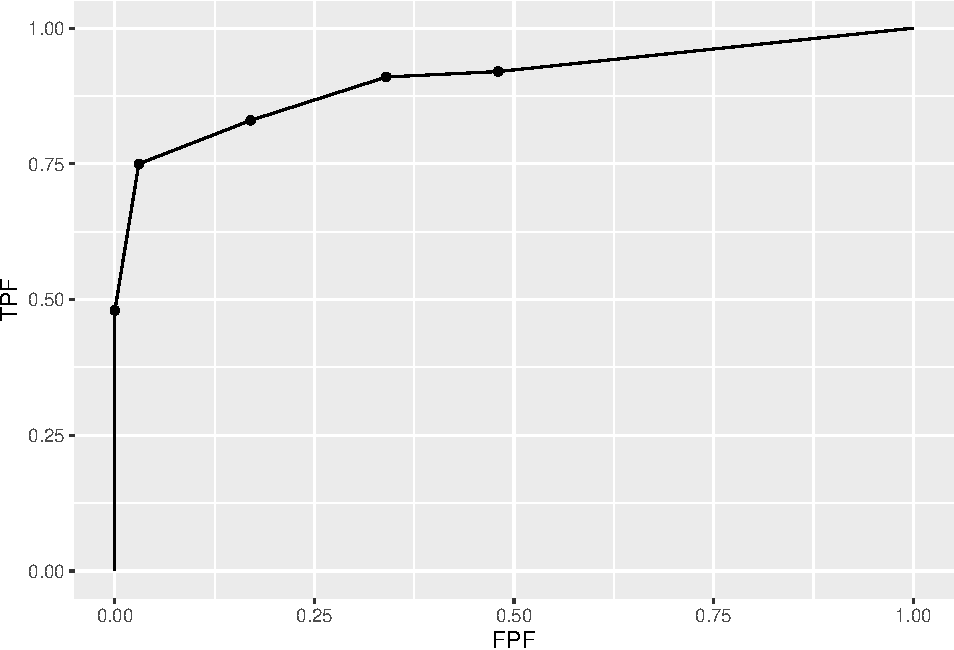
\includegraphics{03-empirical_files/figure-latex/unnamed-chunk-4-1.pdf}

Shown next is calculation of the figure of merit for this dataset. Note that in function \texttt{UtilFigureOfMerit()} the \texttt{FOM} argument has to be set to \texttt{HrAuc}, for highest rating AUC.{]}.

\begin{Shaded}
\begin{Highlighting}[]
\FunctionTok{UtilFigureOfMerit}\NormalTok{(dataset04, }\AttributeTok{FOM =} \StringTok{"HrAuc"}\NormalTok{)}
\CommentTok{\#\textgreater{}         rdr1    rdr3    rdr4    rdr5}
\CommentTok{\#\textgreater{} trt1 0.90425 0.79820 0.81175 0.86645}
\CommentTok{\#\textgreater{} trt2 0.86425 0.84470 0.82050 0.87160}
\CommentTok{\#\textgreater{} trt3 0.81295 0.81635 0.75275 0.85730}
\CommentTok{\#\textgreater{} trt4 0.90235 0.83150 0.78865 0.87980}
\CommentTok{\#\textgreater{} trt5 0.84140 0.77300 0.77115 0.84800}
\end{Highlighting}
\end{Shaded}

\hypertarget{empirical-AFROC}{%
\section{The alternative FROC (AFROC) plot}\label{empirical-AFROC}}

\begin{itemize}
\tightlist
\item
  Fig. 4 in \citep{bunch1977free} anticipated another way of visualizing FROC data. I subsequently termed this the \emph{alternative FROC (AFROC)} plot \citep{chakraborty1989maximum}.
\item
  The empirical AFROC is defined as the plot of \(\text{LLF}(\zeta_r)\) along the ordinate vs.~\(\text{FPF}(\zeta_r)\) along the abscissa.
\item
  \(\text{LLF}_r \equiv \text{LLF}(\zeta_r)\), the ordinate of the FROC plot, was defined in Eqn. \eqref{eq:empirical-LLFr}.
\item
  \(\text{FPF}_r \equiv \text{FPF}(\zeta_r)\), the abscissa of the ROC plot, was defined in Eqn. \eqref{eq:empirical-fpf}.
\end{itemize}

\hypertarget{empirical-definition-empirical-auc-afroc}{%
\subsection{Definition: empirical AFROC plot and AUC}\label{empirical-definition-empirical-auc-afroc}}

The empirical AFROC plot connects adjacent operating points \(\left( \text{FPF}_r, \text{LLF}_r \right )\), including the origin (0,0) and (1,1), with straight lines. The area under this plot is the empirical AFROC AUC, denoted \(A_{\text{AFROC}}\).

Key points:

\begin{itemize}
\tightlist
\item
  The ordinates (LLF) of the FROC and AFROC are identical.
\item
  The abscissa (FPF) of the ROC and AFROC are identical.
\item
  The AFROC is a hybrid plot incorporating aspects of both ROC and FROC plots.
\item
  The AFROC is constrained to within the unit square.
\end{itemize}

\begin{quote}
Prof.~Richard Swensson did not like my choice of the word ``alternative'' in naming this operating characteristic. I had no idea in 1989 how important this plot would later turn out to be, otherwise a more meaningful name might have been proposed. To anticipate the central message of this book, the AUC based on this plot (and weighted versions of it introduced below), are superior to the FROC-AUC and the ROC-AUC in terms of statistical power and reliability (the FROC-AUC is especially unreliable).
\end{quote}

\hypertarget{empirical-AFROC-constrained}{%
\subsection{The observed end-point of the AFROC and its constrained property}\label{empirical-AFROC-constrained}}

According to Eqn. \eqref{eq:empirical-fpf} the abscissa of the observed end-point \(FPF_1 \leq 1\) and according to Eqn. \eqref{eq:empirical-LLF1a} the ordinate of the observed end-point \(\text{LLF}_1 \leq 1\). It follows that the observed end-point of the AFROC satisfies the constrained end-point property, i.e., it lies below-left the (1,1) corner of the plot.

\hypertarget{empirical-afroc-plot-illustration}{%
\subsection{Illustration with a dataset}\label{empirical-afroc-plot-illustration}}

The following code uses \texttt{dataset04} to illustrate an empirical AFROC plot for treatment 1 and reader 1.

\begin{Shaded}
\begin{Highlighting}[]
\NormalTok{ret }\OtherTok{\textless{}{-}} \FunctionTok{PlotEmpiricalOperatingCharacteristics}\NormalTok{(}
\NormalTok{  dataset04, }
  \AttributeTok{trts =} \DecValTok{1}\NormalTok{, }\AttributeTok{rdrs =} \DecValTok{1}\NormalTok{, }\AttributeTok{opChType =} \StringTok{"AFROC"}\NormalTok{)}
\FunctionTok{print}\NormalTok{(ret}\SpecialCharTok{$}\NormalTok{Plot)}
\end{Highlighting}
\end{Shaded}

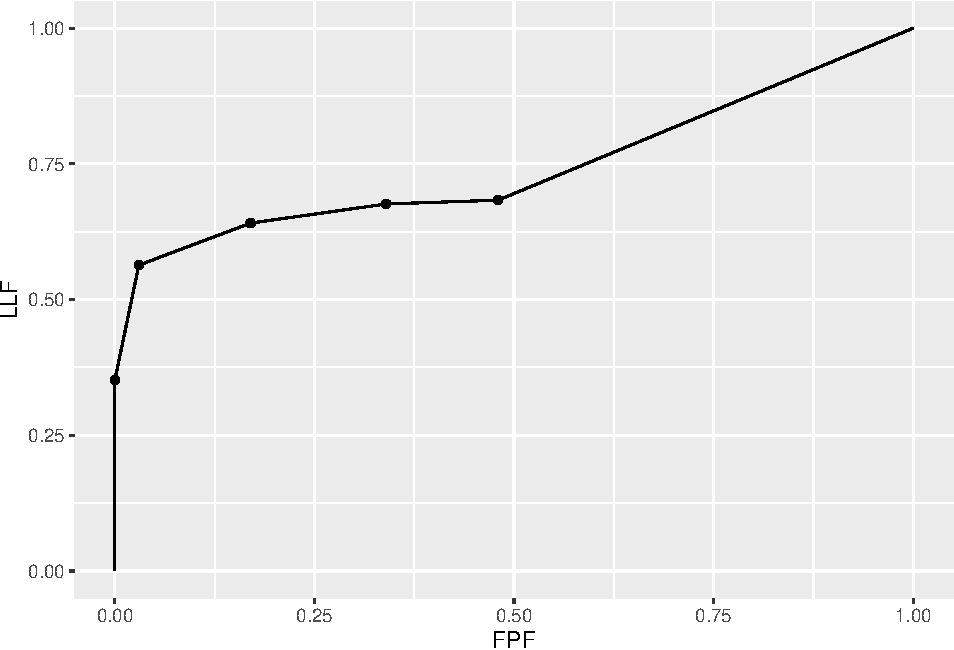
\includegraphics{03-empirical_files/figure-latex/unnamed-chunk-7-1.pdf}

Shown next are the figures of merit for this dataset for all treatment reader combinations.

\begin{Shaded}
\begin{Highlighting}[]
\FunctionTok{UtilFigureOfMerit}\NormalTok{(dataset04, }\AttributeTok{FOM =} \StringTok{"AFROC"}\NormalTok{)}
\CommentTok{\#\textgreater{}           rdr1      rdr3      rdr4      rdr5}
\CommentTok{\#\textgreater{} trt1 0.7427113 0.7104930 0.7003169 0.7909859}
\CommentTok{\#\textgreater{} trt2 0.7586972 0.7161620 0.7225352 0.7927465}
\CommentTok{\#\textgreater{} trt3 0.6983451 0.6955282 0.6777817 0.7547535}
\CommentTok{\#\textgreater{} trt4 0.7817606 0.7234507 0.7132746 0.8136268}
\CommentTok{\#\textgreater{} trt5 0.7169718 0.6690845 0.6587324 0.7682042}
\end{Highlighting}
\end{Shaded}

\hypertarget{empirical-wAFROC}{%
\section{The weighted-AFROC plot (wAFROC) plot}\label{empirical-wAFROC}}

The AFROC ordinate defined in Eqn. \eqref{eq:empirical-LLFr} gives equal importance to every lesion in a case. A case with more lesions will have more influence on the AFROC (see next section for an explicit demonstration of this fact). This is undesirable since each case (i.e., patient) should get equal importance in the analysis -- as with ROC analysis, one wishes to draw conclusions about the population of cases and each case is an equally valid sample from the population. In particular, one does not want the analysis to be skewed towards cases with greater numbers of lesions. \footnote{Historical note: I became aware of how serious this issue could be when a researcher contacted me about using FROC methodology for nuclear medicine bone scan images, where the number of lesions on diseased cases can vary from a few to a hundred!}

Another issue is that the AFROC assigns equal \emph{clinical} importance to each lesion in a case. Lesion weights were introduced \citep{RN1385} to allow for the possibility that the clinical importance of finding a lesion might be lesion-dependent \citep{RN1966}. For example, it is possible that a diseased cases has lesions of two types with differing clinical importance; the figure-of-merit should give more credit to finding the more clinically important one. Clinical importance could be defined as the mortality associated with the specific lesion type; these can be obtained from epidemiological studies \citep{desantis2011breast}.

Let \(W_{k_2 l_2} \geq 0\) denote the \emph{weight} (i.e., short for clinical importance) of lesion \(l_2\) in diseased case \(k_2\) (since weights are only applicable to diseased cases one can, without ambiguity, drop the case-level and location-level truth subscripts, i.e., the notation \(W_{k_2 2 l_2 2}\) would be superfluous). For each diseased case \(k_2 2\) the weights are subject to the constraint:

\begin{equation}
\sum_{l_2 =1 }^{L_{k_2 2}} W_{k_2 l_2} = 1
\label{eq:empirical-weights-constraint}
\end{equation}

The weighted lesion localization fraction \(\text{wLLF}_r\) is defined by \citep{RN2484}:

\begin{equation}
\text{wLLF}_r \equiv \text{wLLF}\left ( \zeta_r \right ) = \frac{1}{K_2}\sum_{k_2=1}^{K_2}\sum_{l_2=1}^{L_{k_2 2}}W_{k_2 l_2} \mathbb{I}\left ( z_{k_2 2 l_2 2} \geq \zeta_r \right )
\label{eq:empirical-wLLFr}
\end{equation}

\hypertarget{empirical-definition-empirical-auc-wafroc}{%
\subsection{The empirical wAFROC plot and AUC}\label{empirical-definition-empirical-auc-wafroc}}

\begin{quote}
The empirical wAFROC plot connects adjacent operating points \(\left ( \text{FPF}_r, \text{wLLF}_r \right )\), including the origin (0,0), with straight lines plus a straight-line segment connecting the observed end-point to (1,1). The area under this plot is the empirical weighted-AFROC AUC, denoted \(A_{\text{wAFROC}}\).
\end{quote}

\hypertarget{empirical-wafroc-plot-illustration}{%
\subsection{Illustration with a dataset}\label{empirical-wafroc-plot-illustration}}

The following code uses \texttt{dataset04} to illustrate an empirical ROC plot for treatment 1 and reader 1.

\begin{Shaded}
\begin{Highlighting}[]
\NormalTok{ret }\OtherTok{\textless{}{-}} \FunctionTok{PlotEmpiricalOperatingCharacteristics}\NormalTok{(}
\NormalTok{  dataset04, }\AttributeTok{trts =} \DecValTok{1}\NormalTok{, }\AttributeTok{rdrs =} \DecValTok{1}\NormalTok{, }\AttributeTok{opChType =} \StringTok{"wAFROC"}\NormalTok{)}
\FunctionTok{print}\NormalTok{(ret}\SpecialCharTok{$}\NormalTok{Plot)}
\end{Highlighting}
\end{Shaded}

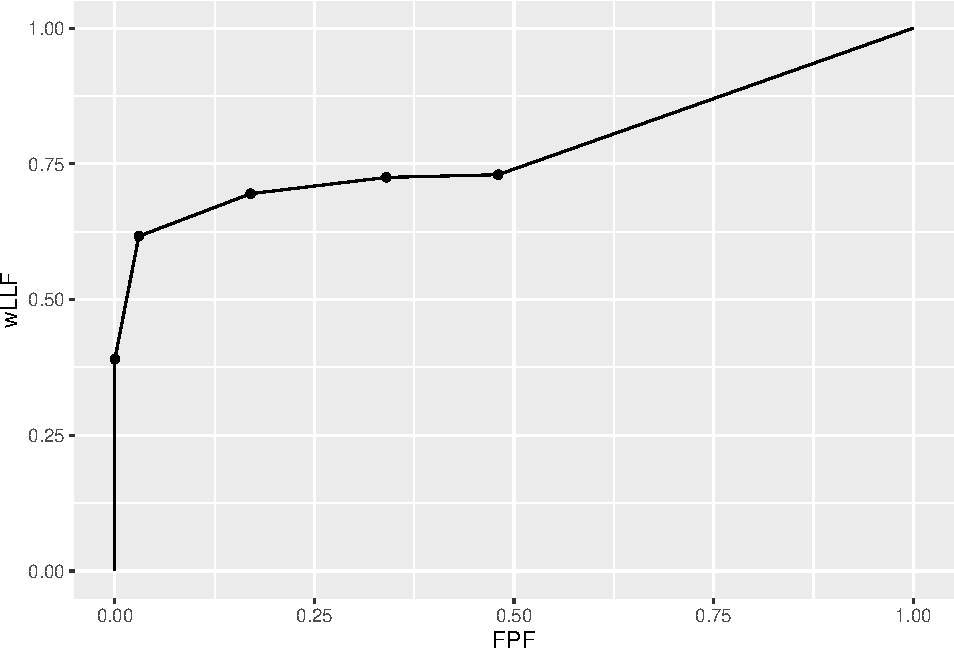
\includegraphics{03-empirical_files/figure-latex/unnamed-chunk-10-1.pdf}

Shown next is calculation of the figure of merit for this dataset.

\begin{Shaded}
\begin{Highlighting}[]
\FunctionTok{UtilFigureOfMerit}\NormalTok{(dataset04, }\AttributeTok{FOM =} \StringTok{"wAFROC"}\NormalTok{)}
\CommentTok{\#\textgreater{}           rdr1      rdr3      rdr4      rdr5}
\CommentTok{\#\textgreater{} trt1 0.7792667 0.7248917 0.7036250 0.8050917}
\CommentTok{\#\textgreater{} trt2 0.7870000 0.7269000 0.7226167 0.8037833}
\CommentTok{\#\textgreater{} trt3 0.7296917 0.7157583 0.6723083 0.7726583}
\CommentTok{\#\textgreater{} trt4 0.8101333 0.7431167 0.6943583 0.8294083}
\CommentTok{\#\textgreater{} trt5 0.7488000 0.6822750 0.6551750 0.7712500}
\end{Highlighting}
\end{Shaded}

\hypertarget{empirical-numerical-understanding}{%
\section{AFROC vs.~wAFROC}\label{empirical-numerical-understanding}}

The fact that the wAFROC gives equal importance to each diseased case while the AFROC gives more importance to diseased cases with more lesions can be illustrated with a fictitious small dataset consisting of \(K_1 = 4\) non-diseased and \(K_2 = 5\) diseased cases. The maximum number of NLs per case is two and the maximum number of lesions per case is three. The first two diseased cases have one lesion each, the third and fourth have two lesions each and the fifth has 3 lesions. Here is how we code the NL and LL z-samples (\texttt{t()} is the \texttt{R} transpose operator). The negative infinities represent unmarked locations. For example, the first non-diseased case has no NL marks, the second has one mark rated 0.5, etc., and the first diseased case has one NL mark rated 1.5, etc. The first lesion in the LL array was rated 0.9. the second was rated -0.2, \ldots, and the 3 lesions in the fifth diseased case were rated 1, 2.5 and 1, respectively.

\begin{Shaded}
\begin{Highlighting}[]
\NormalTok{NL }\OtherTok{\textless{}{-}} \FunctionTok{t}\NormalTok{(}\FunctionTok{array}\NormalTok{(}\FunctionTok{c}\NormalTok{(}\SpecialCharTok{{-}}\ConstantTok{Inf}\NormalTok{, }\SpecialCharTok{{-}}\ConstantTok{Inf}\NormalTok{,  }
                 \FloatTok{0.5}\NormalTok{, }\SpecialCharTok{{-}}\ConstantTok{Inf}\NormalTok{, }
                 \FloatTok{0.7}\NormalTok{, }\FloatTok{0.6}\NormalTok{, }
                \SpecialCharTok{{-}}\FloatTok{0.3}\NormalTok{, }\SpecialCharTok{{-}}\ConstantTok{Inf}\NormalTok{, }
                 \FloatTok{1.5}\NormalTok{, }\SpecialCharTok{{-}}\ConstantTok{Inf}\NormalTok{, }
                \SpecialCharTok{{-}}\ConstantTok{Inf}\NormalTok{, }\SpecialCharTok{{-}}\ConstantTok{Inf}\NormalTok{, }
                \SpecialCharTok{{-}}\ConstantTok{Inf}\NormalTok{, }\SpecialCharTok{{-}}\ConstantTok{Inf}\NormalTok{, }
                \SpecialCharTok{{-}}\ConstantTok{Inf}\NormalTok{, }\SpecialCharTok{{-}}\ConstantTok{Inf}\NormalTok{,}
              \SpecialCharTok{{-}}  \ConstantTok{Inf}\NormalTok{, }\SpecialCharTok{{-}}\ConstantTok{Inf}\NormalTok{), }\AttributeTok{dim =} \FunctionTok{c}\NormalTok{(}\DecValTok{2}\NormalTok{,}\DecValTok{9}\NormalTok{)))}
\NormalTok{LL }\OtherTok{\textless{}{-}} \FunctionTok{t}\NormalTok{(}\FunctionTok{array}\NormalTok{(}\FunctionTok{c}\NormalTok{(}\FloatTok{0.9}\NormalTok{, }\SpecialCharTok{{-}}\ConstantTok{Inf}\NormalTok{, }\SpecialCharTok{{-}}\ConstantTok{Inf}\NormalTok{, }
               \SpecialCharTok{{-}}\FloatTok{0.2}\NormalTok{, }\SpecialCharTok{{-}}\ConstantTok{Inf}\NormalTok{,}\SpecialCharTok{{-}}\ConstantTok{Inf}\NormalTok{, }
                \FloatTok{1.6}\NormalTok{, }\SpecialCharTok{{-}}\ConstantTok{Inf}\NormalTok{, }\SpecialCharTok{{-}}\ConstantTok{Inf}\NormalTok{, }
                  \DecValTok{3}\NormalTok{,    }\DecValTok{2}\NormalTok{, }\SpecialCharTok{{-}}\ConstantTok{Inf}\NormalTok{, }
                  \DecValTok{1}\NormalTok{,    }\FloatTok{2.5}\NormalTok{,  }\DecValTok{1}\NormalTok{), }\AttributeTok{dim =} \FunctionTok{c}\NormalTok{(}\DecValTok{3}\NormalTok{,}\DecValTok{5}\NormalTok{)))}
\end{Highlighting}
\end{Shaded}

The z-samples are converted to a dataset \texttt{frocData} as shown next:

\begin{Shaded}
\begin{Highlighting}[]
\NormalTok{frocData }\OtherTok{\textless{}{-}} \FunctionTok{Df2RJafrocDataset}\NormalTok{(NL, LL, }\AttributeTok{perCase =} \FunctionTok{c}\NormalTok{(}\DecValTok{1}\NormalTok{,}\DecValTok{1}\NormalTok{,}\DecValTok{2}\NormalTok{,}\DecValTok{2}\NormalTok{,}\DecValTok{3}\NormalTok{))}
\end{Highlighting}
\end{Shaded}

In the above code \texttt{perCase\ =\ c(1,1,2,2,3)} specifies the number of lesions per case: 1 in the first diseased case, 1 in the second, 2 in the third, \ldots, and 3 in the fifth. The function \texttt{Df2RJafrocDataset()} generates the dataset object.

The lesion weights are specified in the following lines.

\begin{Shaded}
\begin{Highlighting}[]
\NormalTok{frocData}\SpecialCharTok{$}\NormalTok{lesions}\SpecialCharTok{$}\NormalTok{weights[}\DecValTok{3}\NormalTok{,] }\OtherTok{\textless{}{-}} \FunctionTok{c}\NormalTok{(}\FloatTok{0.1}\NormalTok{, }\FloatTok{0.9}\NormalTok{, }\SpecialCharTok{{-}}\ConstantTok{Inf}\NormalTok{)}
\NormalTok{frocData}\SpecialCharTok{$}\NormalTok{lesions}\SpecialCharTok{$}\NormalTok{weights[}\DecValTok{4}\NormalTok{,] }\OtherTok{\textless{}{-}} \FunctionTok{c}\NormalTok{(}\FloatTok{0.9}\NormalTok{, }\FloatTok{0.1}\NormalTok{, }\SpecialCharTok{{-}}\ConstantTok{Inf}\NormalTok{)}
\NormalTok{frocData}\SpecialCharTok{$}\NormalTok{lesions}\SpecialCharTok{$}\NormalTok{weights[}\DecValTok{5}\NormalTok{,] }\OtherTok{\textless{}{-}} \FunctionTok{c}\NormalTok{(}\FloatTok{0.3}\NormalTok{, }\FloatTok{0.4}\NormalTok{, }\FloatTok{0.3}\NormalTok{)}
\end{Highlighting}
\end{Shaded}

The first and second diseased cases, which have only one lesion each, are assigned unit weights by default. The first lesion in the third diseased case has weight 0.1 and the second has weight 0.9 -- notice that the weights sum to unity. The fourth diseased cases has the lesion weights reversed, 0.9 and 0.1. The three lesions in the fifth diseased case are assigned weights 0.3. 0.4 and 0.3.

\hypertarget{nl-and-ll-z-samples}{%
\subsection{NL and LL z-samples}\label{nl-and-ll-z-samples}}

Shown next is the \texttt{NL} z-samples array; it has 9 rows, corresponding to the total number of cases (the first four correspond to non-diseased cases and the rest to diseased cases) and 2 columns, corresponding to the maximum number of NLs per case.

\begin{verbatim}
#> NL z-samples:
#>       [,1] [,2]
#>  [1,] -Inf -Inf
#>  [2,]  0.5 -Inf
#>  [3,]  0.7  0.6
#>  [4,] -0.3 -Inf
#>  [5,]  1.5 -Inf
#>  [6,] -Inf -Inf
#>  [7,] -Inf -Inf
#>  [8,] -Inf -Inf
#>  [9,] -Inf -Inf
\end{verbatim}

Shown next is the \texttt{LL} z-samples array; it has 5 rows, corresponding to the total number of diseased cases, and 3 columns, corresponding to the maximum number of LLs per case:

\begin{verbatim}
#> LL z-samples:
#>      [,1] [,2] [,3]
#> [1,]  0.9 -Inf -Inf
#> [2,] -0.2 -Inf -Inf
#> [3,]  1.6 -Inf -Inf
#> [4,]  3.0  2.0 -Inf
#> [5,]  1.0  2.5    1
\end{verbatim}

\hypertarget{lesion-weights}{%
\subsection{Lesion weights}\label{lesion-weights}}

Show next is the lesion weights array:

\begin{verbatim}
#> lesion weights:
#>      [,1] [,2] [,3]
#> [1,]  1.0 -Inf -Inf
#> [2,]  1.0 -Inf -Inf
#> [3,]  0.1  0.9 -Inf
#> [4,]  0.9  0.1 -Inf
#> [5,]  0.3  0.4  0.3
\end{verbatim}

The negative infinities represent missing values.

\hypertarget{fpf}{%
\subsection{FPF}\label{fpf}}

Shown next is the \texttt{FP} z-samples array. Since FPs are only possible on non-diseased cases, this is a length 4 row-vector. Each value is the maximum of the two \texttt{NL} z-samples for the corresponding non-diseased case. As an example, for case \#3 the maximum of the two \texttt{NL} values is 0.7.

\begin{verbatim}
#> FP z-samples:
#> [1] -Inf  0.5  0.7 -0.3
\end{verbatim}

Here are the sorted \texttt{FP} z-samples.

\begin{verbatim}
#> [1] -Inf -0.3  0.5  0.7
\end{verbatim}

The sorting makes it easy to construct the \texttt{FPF} values, shown next.

\begin{verbatim}
#> FPF values:
#>  0.000 0.000 0.000 0.000 0.000 0.000 0.000 0.250 0.500 0.500 0.750 1.000
\end{verbatim}

The first non-zero \texttt{FPF} value is \(0.25 = 1/4\), which occurs when a conceptual sliding threshold is lowered past the highest \texttt{FP} value, namely 0.7. (The 0.25 comes from 1 \texttt{FP} case divided by 4 non-diseased cases.) The next \texttt{FPF} value is \(0.5 = 2/4\), which occurs when the sliding threshold is lowered past the next-highest \texttt{FP} value, namely 0.5. The next \texttt{FPF} value is 0.75 and the last \texttt{FPF} value is unity.

\hypertarget{llf}{%
\subsection{LLF}\label{llf}}

Here are the sorted \texttt{LL} z-samples.

\begin{verbatim}
#>  [1] -Inf -Inf -Inf -Inf -Inf -Inf -Inf -0.2  0.9  1.0  1.0  1.6  2.0  2.5  3.0
\end{verbatim}

The \texttt{LLF} values are shown next.

\begin{verbatim}
#> LLF values:
#>  0.000 0.111 0.222 0.333 0.444 0.667 0.778 0.778 0.778 0.889 0.889 1.000
\end{verbatim}

The first non-zero \texttt{LLF} value is 0.111, which occurs when the sliding threshold is lowered past the highest \texttt{LL} value, namely 3. The 0.111 comes from 1 LL divided by 9, the total number of lesions. The next \texttt{LLF} value is 0.222, which occurs when the sliding threshold is lowered past the next-highest \texttt{LL} value, namely 2.5 (2/9 = 0.222). The next \texttt{LLF} value is 0.333, which occurs when the sliding threshold is lowered past 2 (3/9 = 0.333), and so on.

\hypertarget{wllf}{%
\subsection{wLLF}\label{wllf}}

The sorted \texttt{LL} z-samples array and the weights are used to construct the \texttt{wLLF} values shown next.

\begin{verbatim}
#> wLLF values:
#>  0.000 0.180 0.260 0.280 0.300 0.420 0.620 0.620 0.620 0.820 0.820 1.000
\end{verbatim}

The first non-zero \texttt{wLLF} value is 0.18, which occurs when the sliding threshold is lowered past the highest \texttt{LL} value, namely 3. Since this comes from lesion \#1 on diseased case \#4, whose weight is 0.9, the corresponding incremental vertical jump is \(1/5*0.9 = 0.18\), which is also the net \texttt{wLLF} value corresponding to the most suspicious lesion crossing the cutoff. Notice that we are dividing by 5, the total number of diseased cases, not 9 as in the \texttt{LLF} example.

The next \texttt{wLLF} value is 0.26, which occurs when the sliding threshold is lowered past the next-highest \texttt{LL} value, namely 2.5, which comes from the 2nd lesion on the fifth diseased case with weight 0.4. The incremental jump in \texttt{wLLF} is \(1/5*0.4 = 0.08\). The net \texttt{wLLF} value corresponding to the two most suspicious lesions crossing the cutoff is \(1/5*0.9 + 1/5*0.4 = 0.26\).

The next \texttt{wLLF} value is 0.280, which occurs when the sliding threshold is lowered past 1.6, which comes from lesion \#1 on diseased case \#3, with weight 0.1, and the net \texttt{wLLF} value corresponding to the three most suspicious lesions crossing the cutoff is \(1/5*0.9 + 1/5*0.4 + 1/5*0.1 = 0.280\), and so on.

The reader should complete these hand-calculations to reproduce all of the \texttt{wLLF} values shown above. The values (FPF, LLF and wLLF) defining the AFROC and wAFROC are summarized here:

\begin{verbatim}
#>     FPF       LLF wLLF
#> 1  0.00 0.0000000 0.00
#> 2  0.00 0.1111111 0.18
#> 3  0.00 0.2222222 0.26
#> 4  0.00 0.3333333 0.28
#> 5  0.00 0.4444444 0.30
#> 6  0.00 0.6666667 0.42
#> 7  0.00 0.7777778 0.62
#> 8  0.25 0.7777778 0.62
#> 9  0.50 0.7777778 0.62
#> 10 0.50 0.8888889 0.82
#> 11 0.75 0.8888889 0.82
#> 12 1.00 1.0000000 1.00
\end{verbatim}

This shows that the empirical AFROC is defined by the following 6 operating points: (0,0), (0,0.7777778), (0.5,0.7777778), (0.5,0.8888889), (0.75, 0.8888889) and (1,1). Likewise, the empirical wAFROC is defined by the following 6 operating points: (0,0), (0,0.62), (0.5,62), (0.5,0.82), (0.75, 0.82) and (1,1). In each case one simply connects neighboring points with straight lines.

The hand-calculations also show why the AFROC gives more importance to diseased cases with more lesions while the wAFROC does not.

\begin{itemize}
\item
  Considering the AFROC, diseased case \#5 with three lesions which contributes three vertical jumps to LLF totaling \(3/9 = 0.333333\) \footnote{The jumps need not be contiguous: they will be contiguous only if the three lesion z-samples are closely spaced such that they are crossed in succession, in any order, by the sliding virtual threshold; otherwise the jumps will be interspersed by jumps from lesions in other cases.}. This is larger than the contribution to LLF of diseased case \#1 with one lesion \(1/9 = 0.11111\).
\item
  Considering the wAFROC, the three lesions on diseased case \#5 contribute \(1/5*0.3 + 1/5*0.4 + 1/5*0.3 = 0.2\) to wLLF, the same as diseased case \#1, \(1/5*1 = 0.2\).
\end{itemize}

Shown in Fig. \ref{fig:plots-afrocPlot-wafrocPlot} are the empirical AFROC and wAFROC plots.

\begin{figure}
\centering
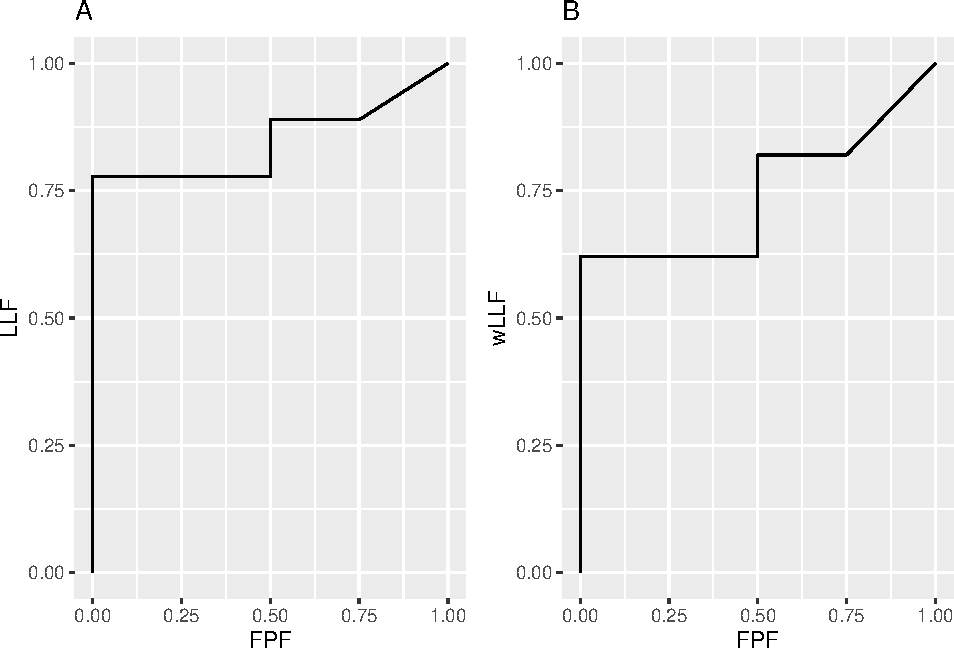
\includegraphics{03-empirical_files/figure-latex/plots-afrocPlot-wafrocPlot-1.pdf}
\caption{\label{fig:plots-afrocPlot-wafrocPlot}Left: AFROC plot; Right: corresponding wAFROC plot.}
\end{figure}

The operating points can be used to numerically calculate the AUCs under the empirical AFROC and wAFROC plots, as done in the following code:

\begin{Shaded}
\begin{Highlighting}[]
\NormalTok{afroc\_auc }\OtherTok{\textless{}{-}} \FloatTok{0.5} \SpecialCharTok{*} \FloatTok{0.7777778} \SpecialCharTok{+} 
  \FloatTok{0.25} \SpecialCharTok{*} \FloatTok{0.8888889} \SpecialCharTok{+} 
  \FloatTok{0.25} \SpecialCharTok{*} \FloatTok{0.8888889} \SpecialCharTok{+}\NormalTok{ (}\DecValTok{1} \SpecialCharTok{{-}} \FloatTok{0.8888889}\NormalTok{) }\SpecialCharTok{*} \FloatTok{0.25} \SpecialCharTok{/}\DecValTok{2}

\NormalTok{wafroc\_auc }\OtherTok{\textless{}{-}} \FloatTok{0.5} \SpecialCharTok{*} \FloatTok{0.62} \SpecialCharTok{+} 
  \FloatTok{0.25} \SpecialCharTok{*} \FloatTok{0.82} \SpecialCharTok{+} 
  \FloatTok{0.25} \SpecialCharTok{*} \FloatTok{0.82} \SpecialCharTok{+} 
\NormalTok{  (}\DecValTok{1} \SpecialCharTok{{-}} \FloatTok{0.82}\NormalTok{) }\SpecialCharTok{*} \FloatTok{0.25} \SpecialCharTok{/}\DecValTok{2}

\FunctionTok{cat}\NormalTok{(}\StringTok{"afroc\_auc ="}\NormalTok{, afroc\_auc,}\StringTok{"}\SpecialCharTok{\textbackslash{}n}\StringTok{"}\NormalTok{)}
\CommentTok{\#\textgreater{} afroc\_auc = 0.8472222}
\FunctionTok{cat}\NormalTok{(}\StringTok{"wafroc\_auc ="}\NormalTok{, wafroc\_auc,}\StringTok{"}\SpecialCharTok{\textbackslash{}n}\StringTok{"}\NormalTok{)}
\CommentTok{\#\textgreater{} wafroc\_auc = 0.7425}
\end{Highlighting}
\end{Shaded}

The same AUC results are obtained using the function \texttt{UtilFigureOfMerit}:

\begin{Shaded}
\begin{Highlighting}[]
\FunctionTok{cat}\NormalTok{(}\StringTok{"AFROC AUC = "}\NormalTok{, }
    \FunctionTok{as.numeric}\NormalTok{(}\FunctionTok{UtilFigureOfMerit}\NormalTok{(frocData, }\AttributeTok{FOM =} \StringTok{"AFROC"}\NormalTok{)),}\StringTok{"}\SpecialCharTok{\textbackslash{}n}\StringTok{"}\NormalTok{)}
\CommentTok{\#\textgreater{} AFROC AUC =  0.8472222}
\FunctionTok{cat}\NormalTok{(}\StringTok{"wAFROC AUC = "}\NormalTok{, }
    \FunctionTok{as.numeric}\NormalTok{(}\FunctionTok{UtilFigureOfMerit}\NormalTok{(frocData, }\AttributeTok{FOM =} \StringTok{"wAFROC"}\NormalTok{)),}\StringTok{"}\SpecialCharTok{\textbackslash{}n}\StringTok{"}\NormalTok{)}
\CommentTok{\#\textgreater{} wAFROC AUC =  0.7425}
\end{Highlighting}
\end{Shaded}

It is seen that the empirical plots consist of upward and rightward jumps starting from the origin (0,0) and ending at (1,1). Each upward jump is associated with a \texttt{LL} z-sample exceeding a virtual threshold. Each rightward jump is associated with a \texttt{FP} z-sample exceeding the threshold. Upward jumps tend to increase the area under the AFROC-based plots and rightward jumps tend to decrease it, i.e., correct decisions are rewarded and incorrect ones are penalized. If there are only upward jumps then the empirical plot rises from the origin to (0,1), where all lesions are correctly localized without any generating FPs and performance is perfect -- the straight-line extension of the plot to (1,1) ensures that the net area is unity. If there are only horizontal jumps the operating point moves from the origin to (1,0), where none of the lesions are localized and every non-diseased case has at least one NL mark and despite the straight line extension to (1,1), the net area is zero. This represents worst possible performance.

\hypertarget{empirical-meanings}{%
\section{Interpretation of AUCs}\label{empirical-meanings}}

\begin{quote}
\begin{itemize}
\tightlist
\item
  The area under the AFROC is the probability that a lesion is rated higher than any mark on a non-diseased case.
\item
  The area under the weighted-AFROC is lesion-weight adjusted probability that a lesion is rated higher than any mark on a non-diseased case.
\end{itemize}
\end{quote}

\hypertarget{empirical-instructive-cases}{%
\section{Instructive examples}\label{empirical-instructive-cases}}

I am including a few extreme cases that I have found to be instructive. These include chance level performance and observers who do not generate any marks.

\hypertarget{empirical-instructive-cases-FROC}{%
\subsection{The FROC}\label{empirical-instructive-cases-FROC}}

The chance level FROC is a ``flat-liner'' hugging the x-axis except for a possible upturn at large NLF. For an observer who does not generate any marks the FROC plot contains but one point, the origin, and \(A_{\text{FROC}}=0\).

\hypertarget{empirical-instructive-cases-ROC}{%
\subsection{The ROC}\label{empirical-instructive-cases-ROC}}

The chance level ROC is the positive diagonal connecting (0,0) to (1,1). There could be several operating points on this diagonal (apart from sampling effects) but \(A_{\text{ROC}}=0.5\).

An observer who does not generate any marks the ROC plot consists of two points, the origin and (1,1) and \(A_{\text{ROC}}=0.5\).

\hypertarget{empirical-instructive-cases-AFROC}{%
\subsection{The AFROC}\label{empirical-instructive-cases-AFROC}}

\hypertarget{empirical-instructive-cases-AFROC-chance-level}{%
\subsubsection{Chance level performance}\label{empirical-instructive-cases-AFROC-chance-level}}

The chance level AFROC is not the line connecting (0,0) to (1,1). This is a serious misconception that I have encountered. A chance level observer will generate a ``flat-liner'' but this time the plot ends at (1,0) and the straight line extension will be a vertical line connecting (1,0) to (1,1) and \(A_{\text{AFROC}}=0\).

\hypertarget{empirical-empirical-instructive-cases-AFROC-no-marks}{%
\subsubsection{Case of no marks}\label{empirical-empirical-instructive-cases-AFROC-no-marks}}

This is a highly interesting and instructive example. The AFROC plot is a straight line connecting (0,0) and (1,1) which could be mistakenly termed as representing chance level performance. This is far from the truth.

\begin{quote}
An expert radiologist successfully screens out non-diseased cases and sees nothing suspicious in any of them -- not mistaking variants of normal anatomy for false lesions on non-diseased cases is a sign of expertise. Suppose the lesions on diseased cases are very difficult to see, even for the expert, so the radiologist does not mark any of them in addition to not marking any NLs on diseased cases. \textbf{The expert radiologist therefore does not report anything, i.e., generates no marks, and the operating point is ``stuck'' at the origin (0,0).} Even in this unusual situation, one would be justified in connecting the origin to (1,1) and claiming area under AFROC is 0.5. The extension gives the radiologist credit for not marking any non-diseased case; of course, the radiologist does not get any credit for marking any of the lesions. An even better radiologist, who finds and marks some of the lesions, will score higher, and AFROC-AUC will exceed 0.5.
\end{quote}

\hypertarget{empirical-instructive-cases-wAFROC}{%
\subsection{The wAFROC}\label{empirical-instructive-cases-wAFROC}}

Similar comments apply to the wAFROC as already described above for AFROC.

\hypertarget{empirical-froc-auc-poor}{%
\section{FROC-AUC is a poor measure}\label{empirical-froc-auc-poor}}

Regarding the ROC-AUC, i.e., \(A_{\text{ROC}}\), as the gold standard against which all other figures of merit should be compared for consistency in orderings, shown next are plots of \(A_{\text{FROC}}\), \(A_{\text{AFROC}}\) and \(A_{\text{wAFROC}}\) vs.~\(A_{\text{ROC}}\) for the dataset used in the previous illustrations.

\hypertarget{plot-of-froc-auc-vs.-roc-auc}{%
\subsection{Plot of FROC AUC vs.~ROC AUC}\label{plot-of-froc-auc-vs.-roc-auc}}

The following is the plot of \(A_{\text{FROC}}\) vs.~\(A_{\text{ROC}}\). There are 20 points on the plot corresponding to 5 treatments and 4 readers. The straight line is a least squares fit. Note the poor correlation and negative slope between \(A_{\text{FROC}}\) and \(A_{\text{ROC}}\), \(R^2\) = 0.0347791, slope = -0.3978636.

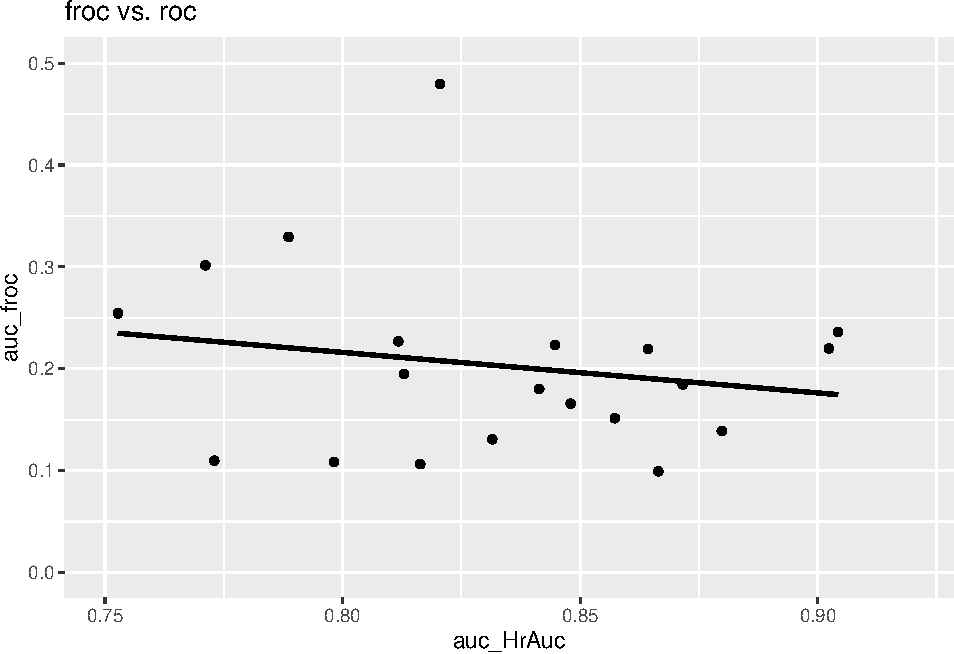
\includegraphics{03-empirical_files/figure-latex/unnamed-chunk-26-1.pdf}

The reason should be fairly obvious. The FROC is unconstrained in the NLF direction and the area under the plot \emph{rewards} an observer who generates more NLs, i.e., as the operating point moves further to the right. (The perfect observer whose FROC plot is the vertical line connecting (0,0) and (0,1) is heavily penalized since \(A_{\text{FROC}} = 0\) for this observer.) One can try to try to avoid this problem by limiting the area under the FROC to that between \(\text{NLF} = 0\) and \(\text{NLF} = x\) where \(x\) is an arbitrarily chosen fixed value -- indeed the partial area procedure has been used by CAD algorithm designers. Since the choice of \(x\) is arbitrary the procedure is subjective. The method would fail for any observer with \(\text{NLF}_{max} < x\) as then the partial area is undefined. This forces the algorithm designer to chose \(x\) as the minimum of all \(\text{NLF}_{max}\) values over all observers and treatments, which would exclude a lot of data and lead to a statistical power penalty.

\hypertarget{plot-of-afroc-auc-vs.-roc-auc}{%
\subsection{Plot of AFROC AUC vs.~ROC AUC}\label{plot-of-afroc-auc-vs.-roc-auc}}

The following is the plot of \(A_{\text{AFROC}}\) vs.~\(A_{\text{ROC}}\). This time there is a strong positive correlation between the two, \(R^2\) = 0.7258723, slope = 0.8649687. The reason is that the AFROC is fully contained in the unit square. An observer who generates more NL marks will yield smaller \(A_{\text{AFROC}}\) -- as the abscissa of the AFROC approaches unity the restriction to the unit square ensures that AUC will decrease.

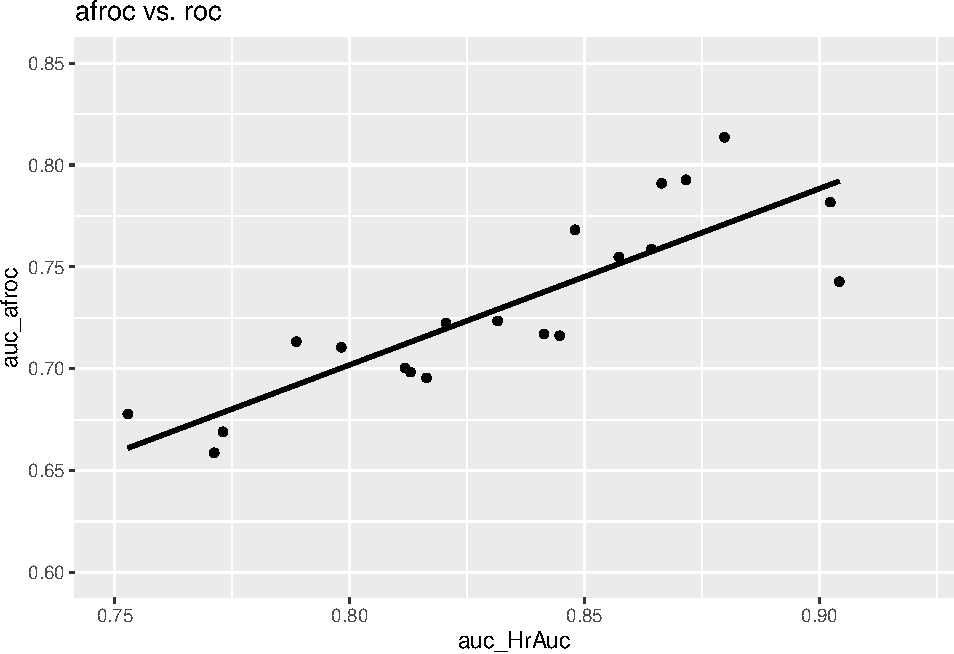
\includegraphics{03-empirical_files/figure-latex/unnamed-chunk-28-1.pdf}

\hypertarget{plot-of-wafroc-auc-vs.-roc-auc}{%
\subsection{Plot of wAFROC AUC vs.~ROC AUC}\label{plot-of-wafroc-auc-vs.-roc-auc}}

The following is the plot of \(A_{\text{wAFROC}}\) vs.~\(A_{\text{ROC}}\). Again, there is a strong positive correlation between the two, \(R^2\) = 0.8569511, slope = 1.0691159. The reason is that the wAFROC is also fully contained in the unit square.

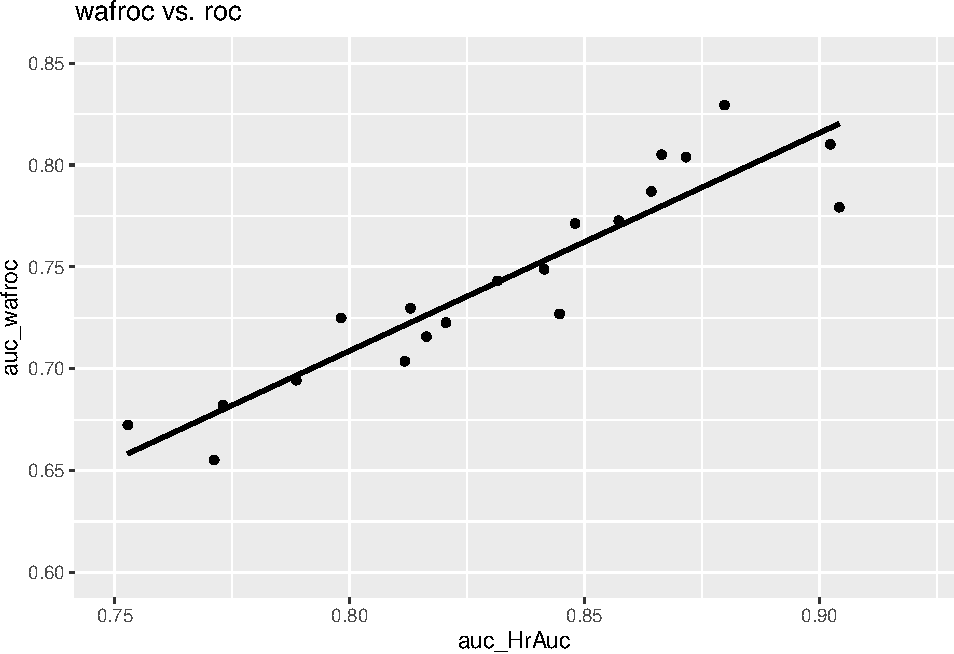
\includegraphics{03-empirical_files/figure-latex/unnamed-chunk-30-1.pdf}

\hypertarget{empirical-AFROC1}{%
\section{The AFROC1 plot}\label{empirical-AFROC1}}

\begin{quote}
Historically the AFROC originally used a different definition of FPF resulting in what is now termed the AFROC1 plot.
\end{quote}

Since NLs can occur on diseased cases it is possible to define an inferred ``FP'' z-sample on a \emph{diseased case} as the maximum of all NL z-samples on the case, or \(-\infty\) if the case has no NLs. The quotes emphasize that this is non-standard usage of ROC terminology since in an ROC study, a FP can only occur on a \emph{non-diseased case}. Since both case-level truth states are allowed, the highest false positive (FP) z-sample for case \(k_t t\), where \(t = 1,2\), is:

\begin{equation}
\left.
\begin{aligned}
\begin{matrix}
FP_{k_1 t}^1=&\max_{l_1} \left ( z_{k_t t l_1 1 } \right ) & \text{if} & l_1 \neq \varnothing\\
FP_{k_t t}^1=&-\infty & \text{if} & l_1 = \varnothing
\end{matrix}
\end{aligned}
\right \}
\label{eq:empirical-FP1}
\end{equation}

The ``1'' superscript below is necessary to distinguish the above definition from that in Eqn. \eqref{eq:empirical-FP}.

\(FP_{k_t t}^1\) is the maximum over all latent NL marks, labeled by the location index \(l_1\), occurring in case \(k_t t\), or \(-\infty\) if \(l_1 = \varnothing\). The corresponding false positive fraction \(FPF_r^1\) is defined by:

\begin{equation}
\left.
\begin{aligned}
FPF_r^1 
&\equiv FPF^1\left ( \zeta_r \right ) \\
&= \frac{1}{K_1+K_2}\sum_{t=1}^{2}\sum_{k_t=1}^{K_t} \mathbb{I}\left ( FP_{k_t t}^1 \geq \zeta_r \right )
\end{aligned}
\right \}
\label{eq:empirical-fpf1}
\end{equation}

Note the differences between Eqn. \eqref{eq:empirical-fpf} and Eqn. \eqref{eq:empirical-fpf1}. The latter counts ``FPs'' on non-diseased \emph{and} diseased cases while Eqn. \eqref{eq:empirical-fpf} counts FPs on \emph{only} non-diseased cases. The denominators in the two equations are different and, unlike the first equation, the second equation is valid even when \(K_1 = 0\). This definition, resulting in the AUCs described next, is useful in applications where all (or almost all) cases are diseased (i.e., all cases have ``targets''). Most machine language applications may fall into this category: for example, a face-recognition algorithm may be used to search for target faces (e.g., known criminals) to be localized in crowd images; there mau be no (or very few) crowd images without any target faces. For these applications the following two empirical characteristics (AFROC1 and wAFROC1) are relevant.

\hypertarget{empirical-definition-empirical-auc-afroc1}{%
\subsection{Empirical AFROC1 plot and AUC}\label{empirical-definition-empirical-auc-afroc1}}

\begin{quote}
The empirical AFROC1 plot connects adjacent operating points \(\left ( FPF_r^1, \text{LLF}_r \right )\), including the origin (0,0) and (1,1), with straight lines. The only difference between AFROC1 plot and the AFROC plot is the x-axis. The area under this plot is the empirical AFROC1 AUC, denoted \(A_{\text{AFROC1}}\) or AFROC1-AUC.
\end{quote}

\hypertarget{empirical-afroc1-plot-illustration}{%
\subsection{Illustration with a dataset}\label{empirical-afroc1-plot-illustration}}

The following code uses \texttt{dataset04} to illustrate an empirical AFROC1 plot for treatment 1 and reader 1. Note that the only difference from an empirical AFROC plot is in the abscissa.

\begin{Shaded}
\begin{Highlighting}[]
\NormalTok{ret }\OtherTok{\textless{}{-}} \FunctionTok{PlotEmpiricalOperatingCharacteristics}\NormalTok{(}
\NormalTok{  dataset04, }
  \AttributeTok{trts =} \DecValTok{1}\NormalTok{, }\AttributeTok{rdrs =} \DecValTok{1}\NormalTok{, }\AttributeTok{opChType =} \StringTok{"AFROC1"}\NormalTok{)}
\FunctionTok{print}\NormalTok{(ret}\SpecialCharTok{$}\NormalTok{Plot)}
\end{Highlighting}
\end{Shaded}

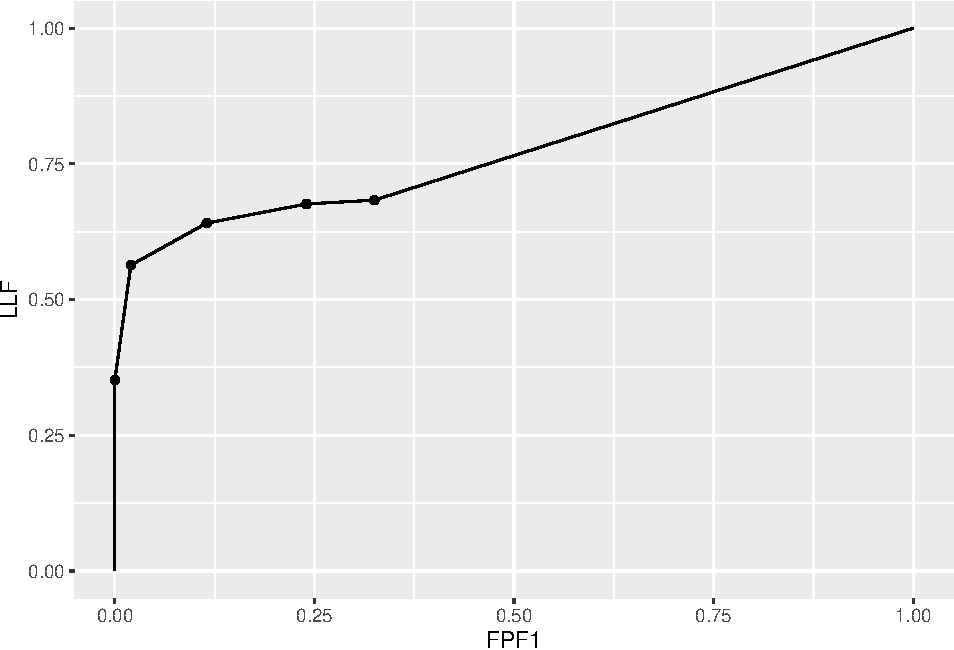
\includegraphics{03-empirical_files/figure-latex/unnamed-chunk-31-1.pdf}

Shown next is calculation of AFROC1-AUC for this dataset.

\begin{Shaded}
\begin{Highlighting}[]
\FunctionTok{UtilFigureOfMerit}\NormalTok{(dataset04, }\AttributeTok{FOM =} \StringTok{"AFROC1"}\NormalTok{)}
\CommentTok{\#\textgreater{}           rdr1      rdr3      rdr4      rdr5}
\CommentTok{\#\textgreater{} trt1 0.7744718 0.7157218 0.7229225 0.7913908}
\CommentTok{\#\textgreater{} trt2 0.7826585 0.7278169 0.7364437 0.7897887}
\CommentTok{\#\textgreater{} trt3 0.7412852 0.6868310 0.6946303 0.7573415}
\CommentTok{\#\textgreater{} trt4 0.8087852 0.7346831 0.7343486 0.8155634}
\CommentTok{\#\textgreater{} trt5 0.7580810 0.6825704 0.6643662 0.7742782}
\end{Highlighting}
\end{Shaded}

\hypertarget{empirical-wAFROC1}{%
\section{The weighted-AFROC1 (wAFROC1) plot}\label{empirical-wAFROC1}}

Similar to the logic for introducing the wAFROC plot as a way of giving equal importance to all diseased cases and allowing the clinical importance of lesions to be modeled by appropriate weights, we introduce a weighted version of the AFROC1, termed the wAFROC1. The ordinate of this plot is the weighted lesion localization fraction \(\text{wLLF}_r\) defined in Eqn. \eqref{eq:empirical-wLLFr}. The abscissa is FPF1, defined in Eqn. \eqref{eq:empirical-fpf1}.

\hypertarget{empirical-definition-empirical-auc-wafroc1}{%
\subsection{Empirical wAFROC1 plot and AUC}\label{empirical-definition-empirical-auc-wafroc1}}

\begin{quote}
The empirical weighted-AFROC1 (wAFROC1) plot connects adjacent operating points \(\left ( FPF_r^1, \text{wLLF}_r \right )\), including the origin (0,0) and (1,1), with straight lines. The only difference between it and the wAFROC plot is in the x-axis. The area under this plot is the empirical weighted-AFROC AUC, denoted \(A_{\text{wAFROC1}}\) or wAFROC1-AUC.
\end{quote}

The wAFROC1-AUC may be preferable as it gives equal importance to each case (or crowd image) regardless of the number of targets contained in it.

\hypertarget{empirical-wafroc1-plot-illustration}{%
\subsection{Illustration with a dataset}\label{empirical-wafroc1-plot-illustration}}

The following code uses \texttt{dataset04} to illustrate an empirical wAFROC1 plot for treatment 1 and reader 1. Note that the only difference from an empirical wAFROC plot is in the abscissa.

\begin{Shaded}
\begin{Highlighting}[]
\NormalTok{ret }\OtherTok{\textless{}{-}} \FunctionTok{PlotEmpiricalOperatingCharacteristics}\NormalTok{(}
\NormalTok{  dataset04, }
  \AttributeTok{trts =} \DecValTok{1}\NormalTok{, }\AttributeTok{rdrs =} \DecValTok{1}\NormalTok{, }\AttributeTok{opChType =} \StringTok{"wAFROC1"}\NormalTok{)}
\FunctionTok{print}\NormalTok{(ret}\SpecialCharTok{$}\NormalTok{Plot)}
\end{Highlighting}
\end{Shaded}

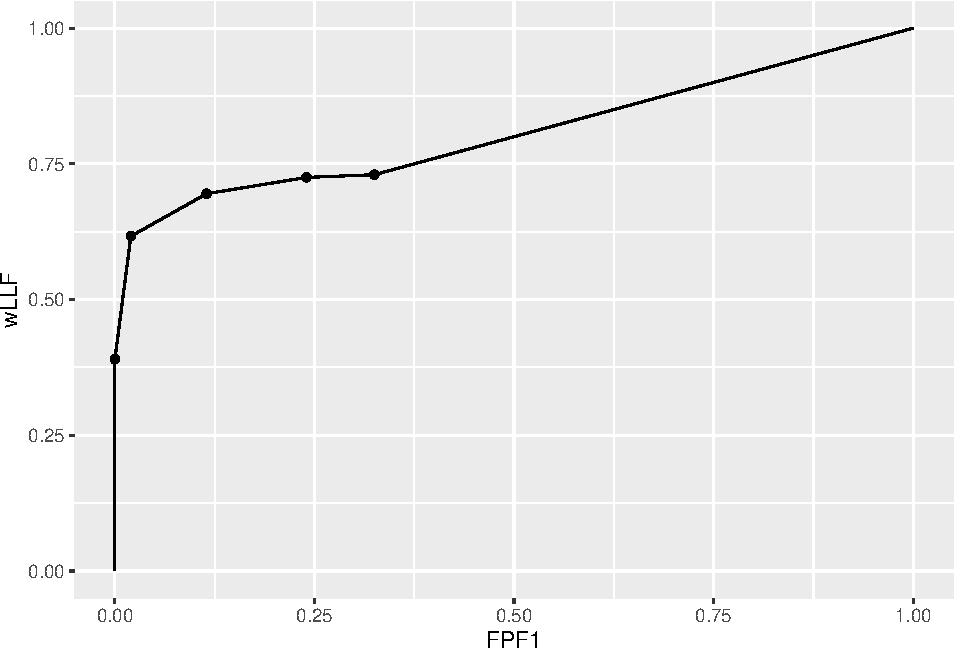
\includegraphics{03-empirical_files/figure-latex/unnamed-chunk-34-1.pdf}

Shown next is calculation of wAFROC1-AUC for this dataset.

\begin{Shaded}
\begin{Highlighting}[]
\FunctionTok{UtilFigureOfMerit}\NormalTok{(dataset04, }\AttributeTok{FOM =} \StringTok{"wAFROC1"}\NormalTok{)}
\CommentTok{\#\textgreater{}           rdr1      rdr3      rdr4      rdr5}
\CommentTok{\#\textgreater{} trt1 0.8068333 0.7298917 0.7262042 0.8058542}
\CommentTok{\#\textgreater{} trt2 0.8084625 0.7379917 0.7363083 0.8010167}
\CommentTok{\#\textgreater{} trt3 0.7680875 0.7075583 0.6890208 0.7743875}
\CommentTok{\#\textgreater{} trt4 0.8348750 0.7533917 0.7160250 0.8308333}
\CommentTok{\#\textgreater{} trt5 0.7857708 0.6953292 0.6605167 0.7774000}
\end{Highlighting}
\end{Shaded}

\hypertarget{empirical-summary}{%
\section{Summary}\label{empirical-summary}}

Here is a summary of the plots defined from FROC data along with my recommendations:

\begin{table}

\caption{\label{tab:empirical-summary}Summary of plots from FROC data. OC = Operating Characteristic. All empirical plots except FROC include a straight line extension from the uppermost observed point to (1,1). Each figure of merit is defined by appending "-AUC" to the name of the corresponding OC}
\centering
\begin{tabular}[t]{l|l|l|l}
\hline
OC & Abscissa & Ordinate & Comments\\
\hline
FROC & NLF & LLF & Not recommended\\
\hline
ROC & FPF & TPF & \\
\hline
AFROC & FPF & LLF & \\
\hline
wAFROC & FPF & wLLF & Recommended when $K_1 \approx K_2$\\
\hline
AFROC1 & FPF1 & LLF & \\
\hline
wAFROC1 & FPF1 & wLLF & Recommended when $K_1 \ll K_2$\\
\hline
\end{tabular}
\end{table}

\hypertarget{empirical-theorem-1}{%
\section{Appendix 1: Proof of formula for wAFROC-AUC}\label{empirical-theorem-1}}

The area \(\text{A}_{wAFROC}\) under the empirical wAFROC plot is obtained by summing the areas of individual trapezoids defined by dropping vertical lines from each pair of adjacent operating points to the x-axis. A sample plot is shown Fig. \ref{fig:empirical-theorems}.

\begin{figure}

{\centering 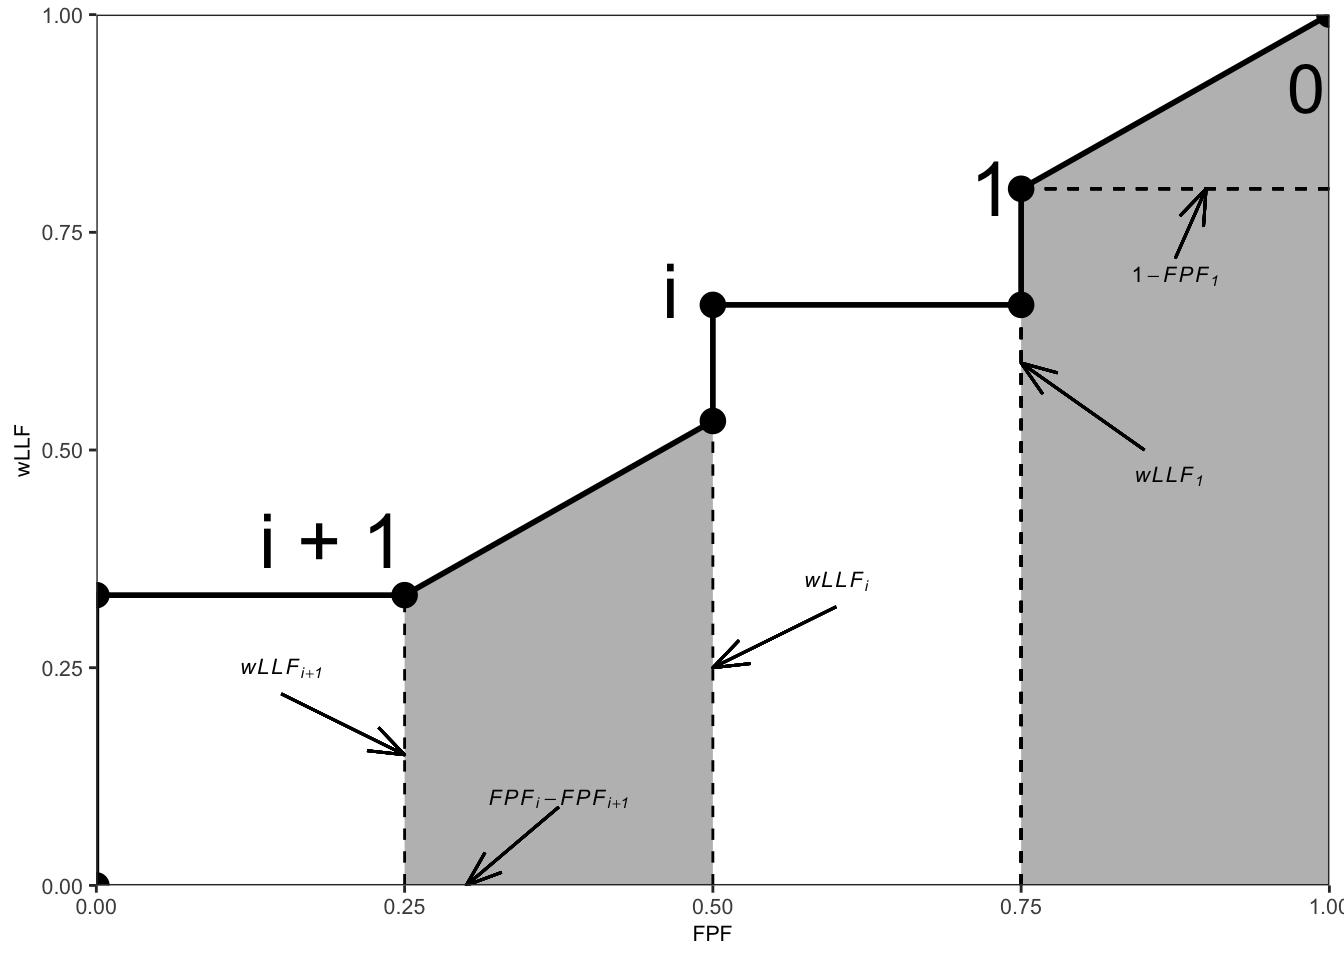
\includegraphics[width=300pt]{images/03-empiricalPlots/proofFigure} 

}

\caption{An example wAFROC plot; from left to right, the two shaded areas correspond to $A_i$ and  $A_0$, respectively, defined below.}\label{fig:empirical-theorems}
\end{figure}

The operating point labeled \(i\) has coordinates \(\left ( \text{FPF}_i, \text{wLLF}_i \right )\) given by Eqn. \eqref{eq:empirical-fpf} and Eqn. \eqref{eq:empirical-wLLFr}.

The area \(A_i\) of the leftmost shaded trapezoid in Fig. \ref{fig:empirical-theorems} is:

\begin{equation}
A_i = \frac{\left (\text{FPF}_i - \text{FPF}_{i+1}\right )\left (\text{wLLF}_i + \text{wLLF}_{i+1}\right )}{2}
\label{eq:empirical-auc-1}
\end{equation}

The weighted lesion localization fraction \(\text{wLLF}_r\) corresponding to threshold \(\zeta_r\) is defined by Eqn. \eqref{eq:empirical-wLLFr}. It follows that:

\begin{equation}
\left. 
\begin{aligned}
A_i =&  \frac{\left (\text{FPF}_i - \text{FPF}_{i+1}\right )}{2} \times \\ 
& \frac{1}{K_2}\left[ \sum_{k_2=1}^{K_2}\sum_{l_2=1}^{L_{k_2 2}}W_{k_2 l_2} \mathbb{I}\left ( z_{k_2 2 l_2 2} \geq \zeta_i \right ) \right. \\
&+ \left. \sum_{k_2=1}^{K_2}\sum_{l_2=1}^{L_{k_2 2}}W_{k_2 l_2} \mathbb{I}\left ( z_{k_2 2 l_2 2} \geq \zeta_{i+1} \right ) \right]  
\end{aligned}
\right \} 
\label{eq:empirical-theorem2}
\end{equation}

Using the probabilistic relation:

\begin{equation}
\mathbb{I}\left ( z_{k_2 2 l_2 2} \geq \zeta_i \right ) = \mathbb{I}\left ( \zeta_{i} \leq z_{k_2 2 l_2 2} < \zeta_{i+1} \right ) + \mathbb{I}\left ( z_{k_2 2 l_2 2} \geq \zeta_{i+1} \right )
\label{eq:empirical-appendix-1}
\end{equation}

we can expand the first term inside the square bracket:

\begin{equation}
\left. 
\begin{aligned}
A_i =&  \frac{\left (\text{FPF}_i - \text{FPF}_{i+1}\right )}{2K_2} \times \\ 
& \left[ \sum_{k_2=1}^{K_2}\sum_{l_2=1}^{L_{k_2 2}}W_{k_2 l_2} \mathbb{I}\left ( \zeta_{i} \leq z_{k_2 2 l_2 2} < \zeta_{i+1} \right ) \right. \\
&+ \sum_{k_2=1}^{K_2}\sum_{l_2=1}^{L_{k_2 2}}W_{k_2 l_2} \mathbb{I}\left ( z_{k_2 2 l_2 2} \geq \zeta_{i+1} \right ) \\ 
&+ \left. \sum_{k_2=1}^{K_2}\sum_{l_2=1}^{L_{k_2 2}}W_{k_2 l_2} \mathbb{I}\left ( z_{k_2 2 l_2 2} \geq \zeta_{i+1} \right ) \right]  
\end{aligned}
\right \} 
\end{equation}

The last two terms are equal, therefore:

\begin{equation}
\left. 
\begin{aligned}
A_i =& \frac{\left (\text{FPF}_i - \text{FPF}_{i+1}\right )}{K_2} \times \\ 
& \left[ \frac{1}{2} \sum_{k_2=1}^{K_2}\sum_{l_2=1}^{L_{k_2 2}}W_{k_2 l_2} \mathbb{I}\left ( \zeta_{i} \leq z_{k_2 2 l_2 2} < \zeta_{i+1} \right ) \right. \\
& +\left. \sum_{k_2=1}^{K_2}\sum_{l_2=1}^{L_{k_2 2}}W_{k_2 l_2} \mathbb{I}\left ( z_{k_2 2 l_2 2} \geq \zeta_{i+1} \right ) \right]  
\end{aligned}
\right \} 
\label{eq:empirical-theorem3}
\end{equation}

The final steps of the proof require that the z-samples be converted to integer ratings, which can be done without loss of ordering information if the number of bins is sufficiently large. Let \(r_{k_t t l_s s}\) denote the integer rating of mark \(k_t tl_s s\), which implies that marks with z-samples satisfying \(\zeta_i \leq z_{k_t tl_s s} < \zeta_{i+1}\), where \(i=0,1,...R\), are rated \(i\) (dummy thresholds \(\zeta_0\) and \(\zeta_{R+1}\) are defined as \(-\infty\) and \(+\infty\), respectively).

From Eqn. \eqref{eq:empirical-fpf} it follows that:

\begin{equation}
\left. 
\begin{aligned}
\text{FPF}_i - \text{FPF}_{i+1}=& \frac{1}{K_1} \left[ \sum_{k_1=1}^{K_1} \mathbb{I}\left ( \max_{l_1} \left (z_{k_1 1 l_1 1}  \right ) \geq \zeta_i \right ) - \sum_{k_1=1}^{K_1} \mathbb{I}\left ( z_{k_1 1 l_1 1} \geq \zeta_{i+1} \right ) \right] \\
=& \frac{1}{K_1} \sum_{k_1=1}^{K_1} \mathbb{I}\left ( \zeta_i \leq \max_{l_1} \left (z_{k_1 1 l_1 1}  \right ) < \zeta_{i+1} \right ) 
\end{aligned}
\right \} 
\label{eq:empirical-theorem4}
\end{equation}

Because of the binning rule, \(\mathbb{I}\left ( \zeta_i \leq \max_{l_1} \left (z_{k_1 1 l_1 1} \right ) < \zeta_{i+1} \right )\) can be replaced by \(\mathbb{I}\left ( \max_{l_1} \left (r_{k_1 1 l_1 1} \right ) = i \right )\), \(\mathbb{I}\left ( \zeta_i \leq z_{k_2 2l_22} < \zeta_{i+1} \right )\) can be replaced by \(\mathbb{I}\left ( r_{k_2 2l_22} = i \right )\) and \(\mathbb{I}\left (z_{k_2 2l_22} \geq \zeta_{i+1} \right )\) can be replaced by \(\mathbb{I}\left (r_{k_2 2l_22} > i \right )\). Then Eqn. \eqref{eq:empirical-theorem2} can be re-written as:

\begin{equation}
\left. 
\begin{aligned}
\text{A}_i =& \frac{1}{K_1K_2}  \sum_{k_2=1}^{K_2} \sum_{l_2=1}^{l_{k_2}}\sum_{k_1=1}^{K_1} \\
&\left [ \frac{1}{2} W_{k_2l_2} \mathbb{I}\left ( \max_{l_1} \left (r_{k_1 1 l_1 1}  \right ) = i  \right )\mathbb{I}\left ( r_{k_2 2 l_2 2} = i\right ) \right. \\
+& \left. \mathbb{I}\left ( \max_{l_1} \left (r_{k_1 1 l_1 1}  \right ) = i  \right )\mathbb{I}\left ( r_{k_2 2 l_2 2} > i \right )  \right ]
\end{aligned}
\right \} 
\label{eq:empirical-theorem5}
\end{equation}

Eqn. \eqref{eq:empirical-theorem5} follows from the property of the indicator function, which constrains \(i\) in the indicator functions inside the square bracket in Eqn. (17) to \(\max_{l_1} \left ( r_{k_1 1 l_1 1} \right )\), where the functions are unity and otherwise they are zero.

Summing over all values of \(i\), one gets for the total area under the empirical wAFROC plot:

\begin{equation}
\begin{aligned}
\text{A}_{wAFROC} =& \frac{1}{K_1K_2}  \sum_{k_2=1}^{K_2} \sum_{l_2=1}^{l_{k_2}}\sum_{k_1=1}^{K_1} W_{k_2l_2} \left( A+B \right)
\end{aligned}
\label{eq:empirical-theorem6}
\end{equation}

where A and B are defined by:

\begin{equation}
\left. 
\begin{aligned}
A =& \mathbb{I}\left ( r_{k_2 2l_2 2} = \max_{l_1} \left (r_{k_1 1l_1 1}  \right )  \right ) \\
B =& \mathbb{I}\left ( r_{k_22 l_2 2} > \max_{l_1} \left (r_{k_11 l_1 1}  \right )  \right )  
\end{aligned}
\right \} 
\label{eq:empirical-theorem6a}
\end{equation}

Defining the Wilcoxon kernel function \(\psi(x,y)\) by:

\begin{equation}
\left. 
\begin{matrix}
\begin{aligned}
&\psi\left( x,y \right) = 1 &  x < y\\
&\psi\left( x,y \right) = 0.5  & x = y \\
&\psi\left( x,y \right) = 0  & x > y
\end{aligned}
\end{matrix}
\right \} 
\label{eq:empirical-wilcoxon-kernel}
\end{equation}

It follows that:

\begin{equation}
\begin{aligned}
\text{A}_{wAFROC} =& \frac{1}{K_1K_2}  \sum_{k_2=1}^{K_2} \sum_{l_2=1}^{l_{k_2}}\sum_{k_1=1}^{K_1} W_{k_2l_2} \psi\left ( \max_{l_1} \left ( r_{k_1 1 l_1 1} \right ) , r_{k_2 2 l_2 2} \right )
\end{aligned}
\label{eq:empirical-theorem7}
\end{equation}

This formula is the wAFROC analog of the familiar Bamber theorem \citep{bamber1975area} relating the empirical AUC under the ROC to the ratings:

\begin{equation}
\text{A}_{ROC} = \frac{1}{K_1K_2}  \sum_{k_2=1}^{K_2} \sum_{k_1=1}^{K_1} \psi\left (  r_{k_11} , r_{k_22} \right )
\label{eq:empirical-bamber-theorem}
\end{equation}

where \(r_{k_11}\) and \(r_{k_22}\) are the ROC ratings of non-diseased case \(k_11\) and diseased case \(k_22\) respectively.

\hypertarget{empirical-theorem-2}{%
\section{Appendix 2: Interpretation of area under straight line extension of wAFROC}\label{empirical-theorem-2}}

We prove that the contribution of the \(i = 0\) term in Eqn. \eqref{eq:empirical-theorem5} is identical to the area under the extension of the wAFROC from the uppermost empirical operating point to (1,1).

According to Eqn. \eqref{eq:empirical-theorem5},

\begin{equation}
\left. 
\begin{aligned}
\text{A}_0 =& \frac{1}{K_1K_2}  \sum_{k_2=1}^{K_2} \sum_{l_2=1}^{l_{k_2}}\sum_{k_1=1}^{K_1} \\
&\left [ \frac{1}{2} W_{k_2l_2} \mathbb{I}\left ( \max_{l_1} \left (r_{k_1 1 l_1 1}  \right ) = 0  \right )\mathbb{I}\left ( r_{k_2 2 l_2 2} = 0 \right ) \right. \\
+& \left. \mathbb{I}\left ( \max_{l_1} \left (r_{k_1 1 l_1 1}  \right ) = 0  \right )\mathbb{I}\left ( r_{k_2 2 l_2 2} > 0 \right )  \right ]
\end{aligned}
\right \} 
\label{eq:empirical-theorem8}
\end{equation}

Rearranging the summations:

\begin{equation}
\left. 
\begin{aligned}
\text{A}_0 =& 
\frac{1}{2} \frac{1}{K_1} \sum_{k_1=1}^{K_1}\mathbb{I}\left ( \max_{l_1} \left (r_{k_1 1 l_1 1}  \right ) = 0  \right ) \frac{1}{K_2} \sum_{k_2=1}^{K_2} \sum_{l_2=1}^{l_{k_2}} W_{k_2l_2} \mathbb{I}\left ( r_{k_2 2 l_2 2} = 0 \right ) \\
+& \frac{1}{K_1} \sum_{k_1=1}^{K_1}\mathbb{I}\left ( \max_{l_1} \left (r_{k_1 1 l_1 1}  \right ) = 0  \right ) \frac{1}{K_2} \sum_{k_2=1}^{K_2} \sum_{l_2=1}^{l_{k_2}} W_{k_2l_2} \mathbb{I}\left ( r_{k_2 2 l_2 2} > 0 \right )
\end{aligned}
\right \} 
\label{eq:empirical-theorem9}
\end{equation}

Consider the term:

\begin{equation}
\frac{1}{K_1} \sum_{k_1=1}^{K_1}\mathbb{I}\left ( \max_{l_1} \left (r_{k_1 1 l_1 1}  \right ) = 0  \right )
\label{eq:empirical-theorem9a}
\end{equation}

Because the indicator function and the summation over \(k_1\) counts the numbers of unmarked non-diseased cases and the division by \(K_1\) yields the corresponding contribution to \(\text{FPF}\), the above term equals the complement of the largest observed \(\text{FPF}\) value, \(\text{FPF}_1\), obtained by cumulating all non-zero ratings, i.e, 1 and above. It follows that:

\begin{equation}
\begin{aligned}
\frac{1}{K_1}\sum_{k_1=1}^{K_1}\mathbb{I}\left ( \max_{l_1} \left (r_{k_1 1 l_1 1}  \right ) = 0  \right ) = 1 - \text{FPF}_1
\end{aligned}
\label{eq:empirical-theorem10}
\end{equation}

Similarly,

\begin{equation}
\begin{aligned}
\frac{1}{K_2}\sum_{k_2=1}^{K_2} \sum_{l_2=1}^{l_{k_2}} W_{k_2l_2} \mathbb{I}\left ( r_{k_2 2 l_2 2}  = 0  \right ) = 1 - \text{wLLF}_1
\end{aligned}
\label{eq:empirical-theorem11}
\end{equation}

Using these expressions, Eqn. \eqref{eq:empirical-theorem9} reduces to:

\begin{equation}
\begin{aligned}
\text{A}_0 = \frac{\left ( 1-\text{FPF}_1 \right ) \left ( 1+\text{wLLF}_1 \right )}{2}
\end{aligned}
\label{eq:empirical-theorem12}
\end{equation}

The area under the straight line extension of the wAFROC from the observed end-point \(\left ( \text{FPF}_1, \text{wLLF}_1 \right )\) to (1,1) equals the area of a rectangle with base \(\left ( 1-\text{FPF}_1 \right )\) and height \(\text{wLLF}_1\) plus the area of a triangle with base \(\left ( 1-\text{FPF}_1 \right )\) and height \((1-\text{wLLF}_1)\):

\begin{equation}
\left. 
\begin{aligned}
\text{Area st. line ext.} =& \left ( 1-\text{FPF}_1 \right )\text{wLLF}_1 
+ \frac{\left( 1-\text{FPF}_1 \right )\left ( 1-\text{wLLF}_1 \right )}{2}  \\
=& \left ( 1-\text{FPF}_1 \right )\left( \text{wLLF}_1 + \frac{\left ( 1-\text{wLLF}_1 \right )}{2} \right) \\
=&
\frac{\left ( 1-\text{FPF}_1 \right ) \left ( 1+\text{wLLF}_1 \right )}{2}
\end{aligned}
\right \} 
\label{eq:empirical-theorem12a}
\end{equation}

which equals the right hand side of Eqn. \eqref{eq:empirical-theorem12}.

\begin{quote}
In other words \(A_0\) is the area under the extension of the wAFROC from observed end-point \(\left ( \text{FPF}_1, \text{wLLF}_1 \right )\) to (1,1).
\end{quote}

According to Eqn. \eqref{eq:empirical-theorem12}, \(A_0\) increases as \(\text{FPF}_1\) decreases, i.e., as more non-diseased cases are \emph{not marked} and as \(\text{wLLF}_1\) increases, i.e., as more lesions, especially those with greater weights, \emph{are marked}. Both observations are in keeping with the behavior of a valid performance measure.

\begin{quote}
\begin{itemize}
\tightlist
\item
  Failure to include the area under the straight-line extension results in not counting the full contribution to the FOM of unmarked non-diseased cases and unmarked lesions. This is best seen by considering the case of a perfect observer.
\item
  For a perfect observer whose plot is the vertical line from (0,0) to (0,1) followed by the horizontal line from (0,1) to (1,1), \emph{the area under the straight-line extension comprises the entire AUC}. Excluding it would yield zero AUC for a perfect observer which is obviously incorrect.
\item
  Stated equivalently, for the perfect observer \(\text{FPF}_1 = 0\) and \(\text{wLLF}_1 = 1\) and then, according to Eqn. \eqref{eq:empirical-theorem12}, the area under the straight line extension is \(A_0 = 1\).
\end{itemize}
\end{quote}

\hypertarget{empirical-summary-computational-formulae}{%
\section{Appendix 3: Summary of computational formulae}\label{empirical-summary-computational-formulae}}

\hypertarget{froc}{%
\subsection{FROC}\label{froc}}

The formula for the area under the empirical FROC plot follows:

\begin{equation}
\begin{aligned}
\text{A}_{FROC} =& \frac{1}{\left ( K_1+K_2 \right )\sum_{k_2=1}^{K_2}L_{k_2 2}}\sum_{k_2=1}^{K_2}\sum_{l_2=1}^{L_{k_2 2}} \left( A+B \right)
\end{aligned}
\label{eq:empirical-computational-froc}
\end{equation}

where A and B are defined by:

\begin{equation}
\left. 
\begin{aligned}
A =& \sum_{k_1=1}^{K_1}\sum_{l_1=1}^{N_{k_1 1}} \mathbb{I} \left ( z_{k_11l_11} \neq  -\infty \right ) \psi\left ( z_{k_11l_11},z_{k_22l_22} \right )\\
B =&\sum_{k_2'=1}^{K_2}\sum_{l_1=1}^{N_{k_2' 2}} \mathbb{I} \left ( z_{z_{k'_22l_11}} \neq  -\infty \right )\psi\left ( z_{k_2'2l_11},z_{k_22l_22} \right )
\end{aligned}
\right \} 
\label{eq:empirical-computational-froc-ab-terms}
\end{equation}

For term A, \(\mathbb{I} \left ( z_{k_11l_11} \neq -\infty \right )\) ensures that only \emph{finite} NL z-samples on non-diseased cases enter the computation (recall that unmarked NLs are unobservable events). Likewise, for term B, \(\mathbb{I} \left ( z_{k'_22l_11} \neq -\infty \right )\) ensures that only \emph{finite} NL z-samples on diseased cases enter the computation. This is not needed for LLs since unmarked LLs are observable events. In term A the double summation compares using the \(\psi\) function all finite NL ratings on \emph{non-diseased} cases \(k_11\) with all lesion ratings on diseased case \(k_22\). In term B the double summation compares all finite NL ratings on \emph{diseased cases} \(k_2'2\) with all lesion ratings on diseased case \(k_22\). The double summation in Eqn. \eqref{eq:empirical-computational-froc} sums over all diseased cases \(k_22\) and all lesions in each diseased case. The final value is divided by the total number of cases and the total number of lesions.

In term B notice the need to distinguish between two indices for diseased cases \(z_{k'_22l_11}\) and \(z_{k_22l_22}\).

The above formula is equivalent to creating two arrays the first containing all finite NL ratings and the second containing all lesion ratings (including unmarked lesions). One cumulates the\(\psi\) function values, using the ratings in the two arrays, and divides by the total number of cases and by the total number of lesions.

The following example uses the same 9-case FROC dataset used earlier. The AUC is calculated two ways: using geometry and using Eqn. \eqref{eq:empirical-computational-froc} implemented in function \texttt{UtilFigureOfMerit}.

\begin{verbatim}
#> numerical integration yields:  0.4074074
#> RJafroc yields:  0.4074074
\end{verbatim}

\hypertarget{roc}{%
\subsection{ROC}\label{roc}}

The ROC-AUC formula is much simpler.

\begin{equation}
\begin{aligned}
\text{A}_{ROC} = \frac{1}{K_1K_2}\sum_{k_1=1}^{K_1}\sum_{k_2=1}^{K_2} \psi\left ( \max_{l_1}\left (z_{k_11l_11} \right ), \max_{l_1l_2}\left (z_{k_22l_11}, z_{k_22l_22}  \right ) \right )
\end{aligned}
\label{eq:empirical-computational-roc}
\end{equation}

The first argument of the \(\psi\) function is the maximum NL rating on a non-diseased case or \(-\infty\) if the case has no NL marks. The second argument is the maximum of all marks, NL or LL, on a diseased case, or \(-\infty\) if the case has no marks. The value of the \(\psi\) function is summed over all non-diseased and diseased cases and divided by \(K_1\) and \(K_2\), analogous to the Bamber theorem Eqn. \eqref{eq:empirical-bamber-theorem}.

\hypertarget{afroc}{%
\subsection{AFROC}\label{afroc}}

The formula for the area under the empirical AFROC plot follows:

\begin{equation}
\begin{aligned}
\text{A}_{AFROC} = \frac{1}{K_1\sum_{k_2=1}^{K_2}L_{k_2 2}}\sum_{k_1=1}^{K_1}\sum_{k_2=1}^{K_2}\sum_{l_2=1}^{L_{k_2 2}} \psi\left ( \max_{l_1}\left (z_{k_11l_11}  \right ),z_{k_22l_22} \right )
\end{aligned}
\label{eq:empirical-computational-afroc}
\end{equation}

The first argument of the \(\psi\) function is the maximum NL rating on a non-diseased case or \(-\infty\) if the case has no NL marks. The second argument is the LL rating on a diseased case. The value of the \(\psi\) function is summed over all non-diseased cases and all lesions and divided by \(K_1\) and the total number of lesions.

\hypertarget{wafroc}{%
\subsection{wAFROC}\label{wafroc}}

The formula for the area under the empirical wAFROC plot follows:

\begin{equation}
\begin{aligned}
\text{A}_{wAFROC} = \frac{1}{K_1K_2}\sum_{k_1=1}^{K_1}\sum_{k_2=1}^{K_2}\sum_{l_2=1}^{L_{k_2 2}} W_{k_2l_2}\psi\left ( \max_{l_1}\left (z_{k_11l_11}  \right ),z_{k_22l_22} \right )
\end{aligned}
\label{eq:empirical-computational-wafroc}
\end{equation}

This is similar to Eqn. \eqref{eq:empirical-computational-afroc} except for the inclusion of the lesion weight term \(W_{k_2l_2}\) inside the summations.

The FOM-statistic \(\text{A}_{wAFROC}\) achieves its highest value, unity, if and only if every lesion is rated higher than any mark on non-diseased cases, for then the \(\psi\) function always yields unity, and the summations yield unity. If, on the other hand, every lesion is rated lower than every mark on every non-diseased case, the \(\psi\) function always yields zero, and the FOM-statistic is zero. Therefore, \(0 \leq \text{A}_{wAFROC} \leq 1\). This shows that \(\text{A}_{wAFROC}\) behaves like a probability and its range is \emph{twice} that of \(\text{A}_{ROC}\); recall that \(0.5 \leq \text{A}_{ROC} \leq 1\) (assuming the observer has equal or better than random performance and the observer does not have the direction of the rating scale reversed). This has the consequence that treatment related differences between \(\text{A}_{wAFROC}\) (i.e., effect sizes) are larger relative to the corresponding ROC effect sizes (just as temperature differences in the Fahrenheit scale are larger than the same differences expressed in the Celsius scale). This has important implications for FROC sample size estimation, see \href{https://dpc10ster.github.io/RJafrocQuickStart/froc-sample-size.html}{sample size chapter} in the \texttt{RJafrocQuickStart} book.

The range \(0 \leq \text{A}_{wAFROC} \leq 1\) is one reason why the ``chance diagonal'' of the AFROC, corresponding to \(\text{A}_{wAFROC} = 0.5\), does \emph{not} reflect chance-level performance. \(\text{A}_{AFROC} = 0.5\) is actually reasonable performance, being exactly in the middle of the allowed range. An example of this was given above for the case of an expert radiologist who does not mark any cases.

Similar comments apply to the AFROC\_AUC, i.e.~\(0 \leq \text{A}_{AFROC} \leq 1\), etc.

\hypertarget{afroc1}{%
\subsection{AFROC1}\label{afroc1}}

\begin{equation}
\begin{aligned}
\text{A}_{AFROC1} =& \frac{1}{\left (K_1 +K_2 \right )\sum_{k_2=1}^{K_2}L_{k_2 2}}\sum_{k_2=1}^{K_2}\sum_{l_2=1}^{L_{k_2 2}} \left( A + B \right)
\end{aligned}
\label{eq:empirical-computational-afroc1}
\end{equation}

where A and B are defined by:

\begin{equation}
\left. 
\begin{aligned}
A =& \sum_{k_1=1}^{K_1}\psi\left ( \max_{l_1}\left (z_{k_11l_11}  \right ),z_{k_22l_22} \right ) \\
B =& \sum_{k_2'=1}^{K_2}\psi\left ( \max_{l_1}\left (z_{k_22l_11}'  \right ),z_{k_22l_22} \right )
\end{aligned}
\right \} 
\label{eq:empirical-computational-afroc1ab}
\end{equation}

The normalization can checked by assuming all NL ratings are less than any LL rating, in which case terms A and B reduce to \(K_1+K_2\) and \(\text{A}_{AFROC1} = 1\):

\begin{equation}
\left. 
\begin{aligned}
\text{A}_{AFROC1} =& \frac{1}{\sum_{k_2=1}^{K_2}L_{k_2 2}}\sum_{k_2=1}^{K_2}\sum_{l_2=1}^{L_{k_2 2}} 1 \\
=& \frac{1}{\sum_{k_2=1}^{K_2}L_{k_2 2}}\sum_{k_2=1}^{K_2}L_{k_2 2} \\
=& 1
\end{aligned}
\right \} 
\label{eq:empirical-computational-afroc1a}
\end{equation}

\hypertarget{wafroc1}{%
\subsection{wAFROC1}\label{wafroc1}}

This is similar to the above expression for AFROC1 except for the presence of the weight term \(W_{k_2l_2}\):

\begin{equation}
\begin{aligned}
\text{A}_{wAFROC1} =& \frac{1}{\left (K_1 + K_2 \right )K_2}\sum_{k_2=1}^{K_2}\sum_{l_2=1}^{L_{k_2 2}} W_{k_2l_2}\left( A+B \right)
\end{aligned}
\label{eq:empirical-computational-wafroc1}
\end{equation}

A and B are as defined in Eqn. \eqref{eq:empirical-computational-afroc1ab}.

\hypertarget{part-the-radiological-search-model-rsm}{%
\part*{The radiological search model (RSM)}\label{part-the-radiological-search-model-rsm}}
\addcontentsline{toc}{part}{The radiological search model (RSM)}

\hypertarget{visual-search}{%
\chapter{Visual Search}\label{visual-search}}

\hypertarget{visual-search-how-much-finished}{%
\section{How much finished}\label{visual-search-how-much-finished}}

100\%

\hypertarget{visual-search-intro}{%
\section{Introduction}\label{visual-search-intro}}

This chapter draws heavily on work by Nodine and Kundel \citep{nodine1987using, kundel2007holistic, kundel2004modeling, kundel1983visual, kundel1978visual}. The author gratefully acknowledges critical insights gained through conversations with Dr.~Claudia Mello-Thoms ca. 2003.

To understand free-response data, specifically how radiologists interpret images, one must come to grips with visual search. Casual usage of everyday terms like ``search'', ``recognition'' and ``detection'' can lead to confusion.

\begin{quote}
Visual search is broadly defined as grouping and labeling parts of an image. In the medical imaging context visual search involves finding lesions and correctly classifying them (as benign or malignant).
\end{quote}

A schema of how radiologists find perform the search task, termed the Kundel-Nodine search model, is described. This model is the basis of the radiological search model (RSM) described in Chapter \ref{rsm}.

\hypertarget{visual-search-grouping-labeling-rois}{%
\section{Grouping and labeling ROIs}\label{visual-search-grouping-labeling-rois}}

Looking at and understanding an image involves grouping and assigning labels to different regions in the image, where the labels correspond to entities that exist in the real world. As an example, if one looks at Fig. \ref{fig:visual-search-us-presidents}, one would group the image into 8 rectangular regions arranged in two rows and 4 columns and label them (from left to right and top to bottom in raster fashion): Franklin Roosevelt, Harry Truman, Lyndon Johnson, Richard Nixon, Jimmy Carter, Ronald Reagan, George H. W. Bush, and the presidential seal. The accuracy of the labeling depends on expertise of the observer: if one were ignorant about American history one would be unable to correctly label them.

\begin{figure}

{\centering 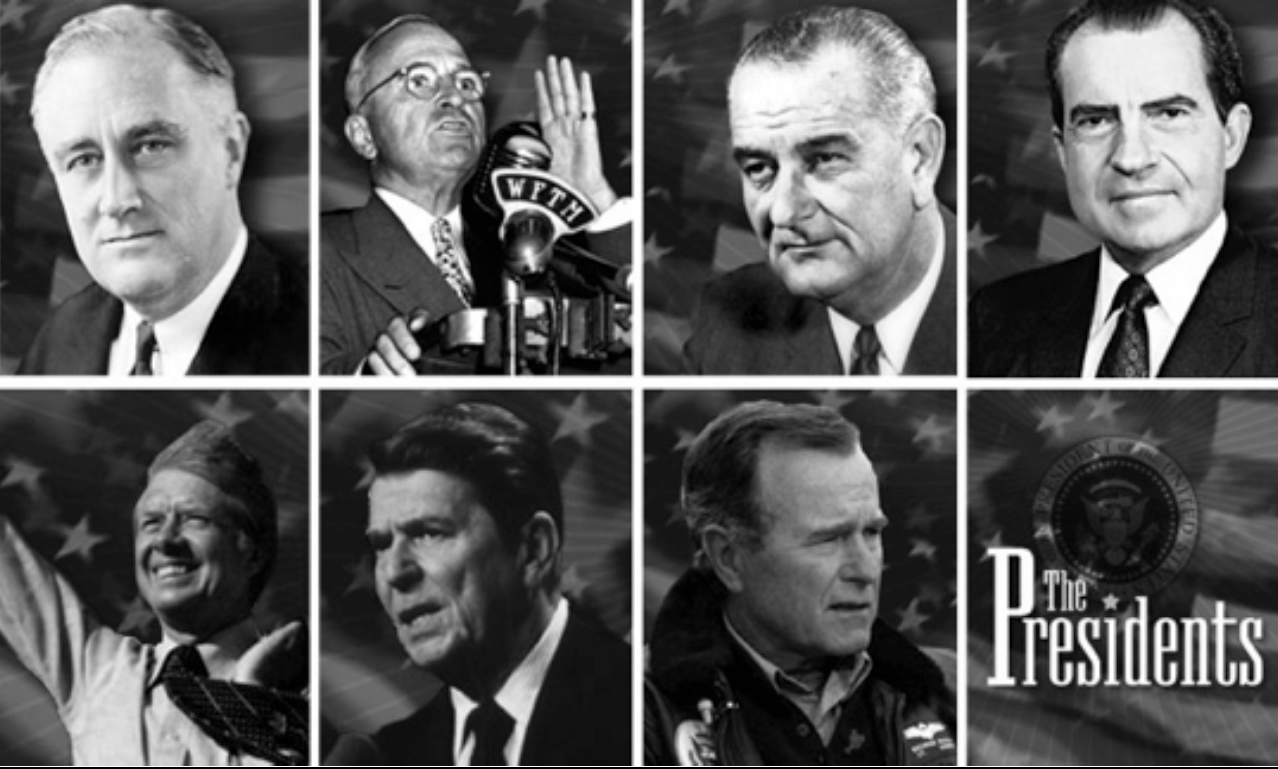
\includegraphics[width=300pt]{images/15-visual-search/usPresidents} 

}

\caption{Grouping and labeling regions of an image.}\label{fig:visual-search-us-presidents}
\end{figure}

Image interpretation in radiology is not fundamentally different. It involves grouping and recognizing areas of the image that have correspondences to the radiologist's knowledge of the underlying anatomy. Most doctors, who need not be radiologists, can look at a chest x-ray and say, ``this is the heart'', ``this is a rib'', ``this is a clavicle'', ``this is the aortic arch'', etc., Fig. \ref{fig:visual-search-chest-images1}. This is because they know the underlying anatomy, Fig. \ref{fig:visual-search-chest-images2} and have a basic understanding of x-ray image formation physics that relates the anatomy to the image.

\begin{figure}

{\centering 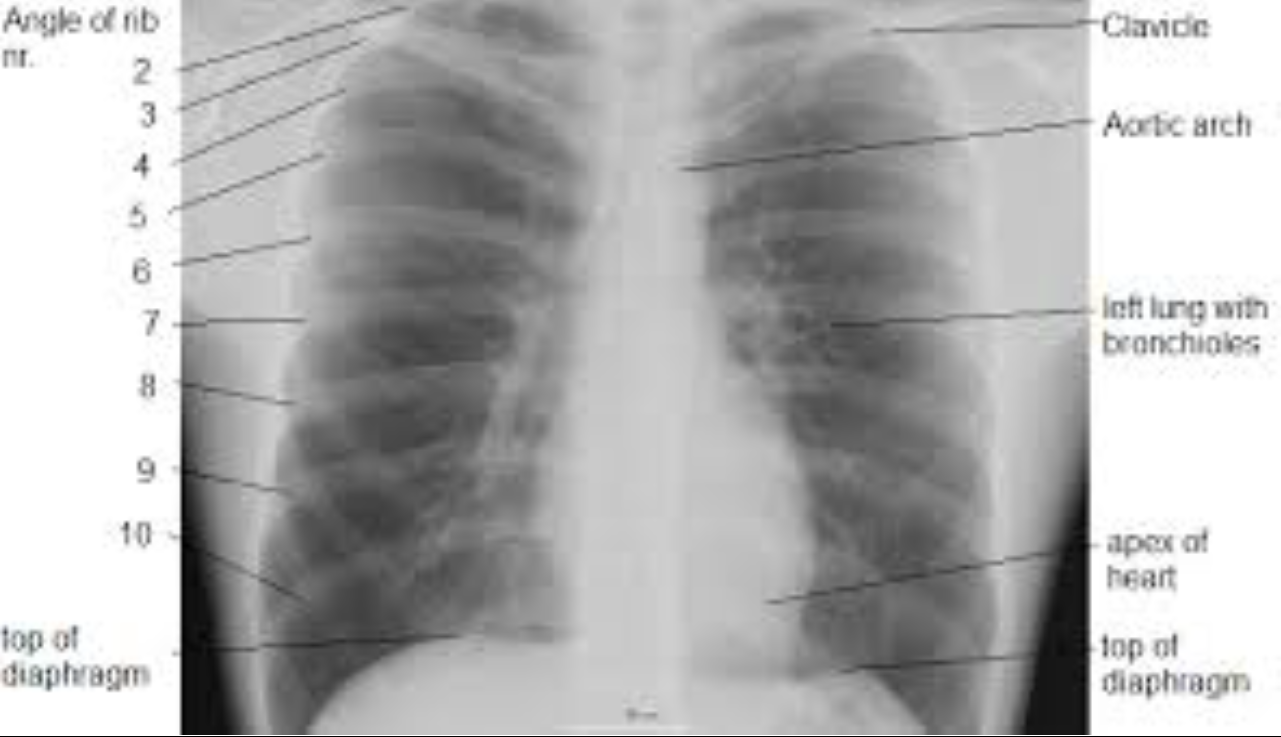
\includegraphics[width=300pt]{images/15-visual-search/chest-imageA} 

}

\caption{Grouping and labeling in radiology.}\label{fig:visual-search-chest-images1}
\end{figure}

\begin{figure}

{\centering 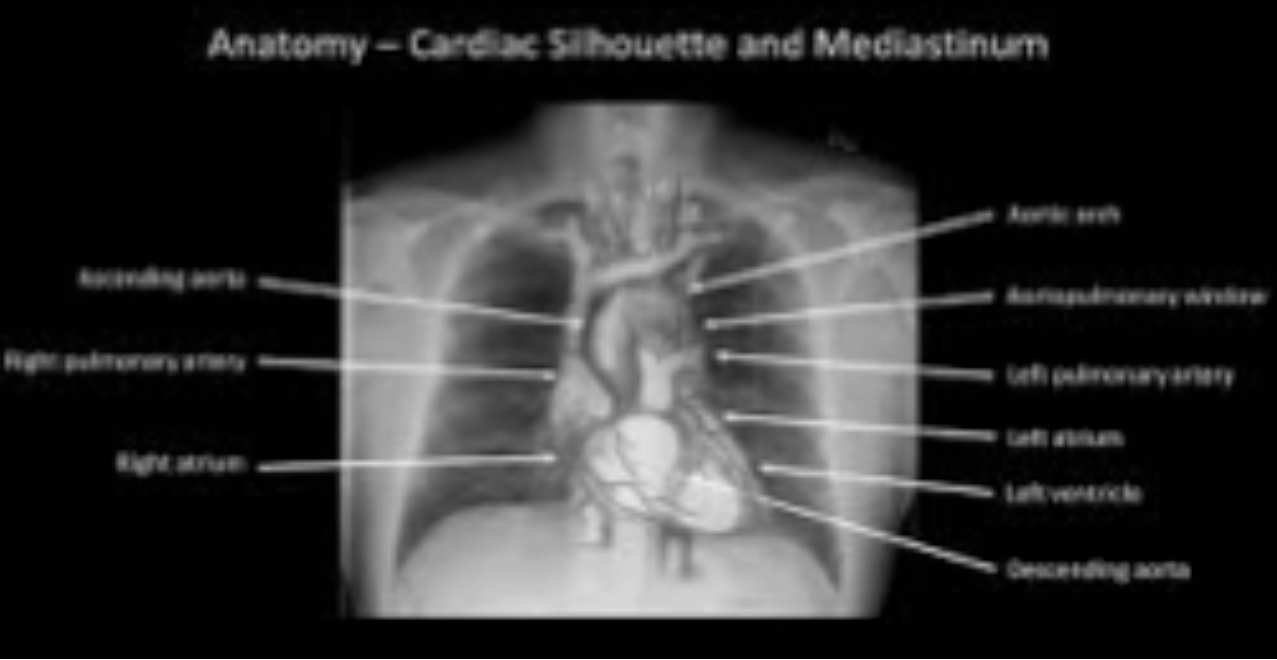
\includegraphics[width=300pt]{images/15-visual-search/chest-imageB} 

}

\caption{Correct grouping and labeling requires knowledge of the underlying anatomy.}\label{fig:visual-search-chest-images2}
\end{figure}

\hypertarget{visual-search-recognition-detection}{%
\section{Lesion-localization vs.~detection}\label{visual-search-recognition-detection}}

The process of grouping and labeling parts of an image is termed \emph{recognition}. Recognition is distinct from detection, which is deciding about the presence of something that is unexpected or the absence of something that is expected, in other words, a deviation from what is expected. An example of detecting the presence of something that is unexpected would be a lung nodule and an example of detecting the absence of something that is expected would be an image of a patient with a missing rib (yes, it does occur, even excluding the biblical Adam).

The terms ``expected'' and ``unexpected'' imply expertise dependent expectations regarding the structure of a generic non-diseased image, which I term a \emph{non-diseased template}, and therefore the ability to recognize clinically relevant perturbations from this template. By ``clinically relevant'' I mean perturbations related to the patient's health outcome: recognizing scratches, dead pixels, artifacts of know origin, and lead patient ID markers do not count. Detection is the presence or absence of something, i.e., the perturbation, which could be anywhere. For example, in Fig. \ref{fig:visual-search-us-presidents}, recognizing a face is equivalent to assigning a row and column index in the image. Specifically, recognizing George H.W. Bush implies pointing to row = 2 and column = 3. Detecting George H.W. Bush implies stating that George H.W. Bush is somewhere in the image. Recognition is an FROC paradigm task while detection is an ROC task.

Instead of recognition (as used by Kundel and Nodine) I prefer the term ``search'', as in ``searching for and finding'' a lesion.

\hypertarget{visual-search-search-classification}{%
\section{Lesion-localization vs.~lesion-classification}\label{visual-search-search-classification}}

Since template perturbations can occur at different locations in the images, the ability to selectively recognize them is related to search expertise. \footnote{A non-expert can trivially recognize any and all perturbations that may be present by claiming all regions in the image are perturbed.} Lesion-localization expertise is the selective ability to locate clinically relevant perturbations that are actually present while minimizing false localizations.

Two important terms are introduced using FROC terminology:

\begin{quote}
Lesion-localization (or finding) expertise is the ability to find latent LLs while minimizing finding latent NLs.

Lesion-classification (or recognition) expertise is the ability to mark LLs while not marking NLs.
\end{quote}

The skills required to find and recognize a nodule in a chest x-ray are different from those required to find and recognize a low-contrast circular or Gaussian shaped artificial nodule against a background of random noise (or even an anthropomorphic phantom). In the former instance the skills of the radiologist are relevant while in the latter they are not. This is the reason why having radiologists interpret random noise images and claiming that this somehow makes it ``clinically relevant'' is incorrect. One might as well use anyone with good eyesight, motivation and training. This paragraph also argues against phantoms as stand-ins for clinical images for ``clinical'' performance assessment. Phantoms are fine in the quality control context but they do not allow radiologists the opportunity to exercise their skills.

\hypertarget{visual-search-kundel-nodine-model}{%
\section{The Kundel - Nodine search model}\label{visual-search-kundel-nodine-model}}

The Kundel-Nodine model \citep{kundel2007holistic, kundel2004modeling} is a schema of events that occur from the radiologist's first glance to the decision about the image.

Assuming the task has been defined (and based on eye-tracking recordings obtained on radiologists while they interpreted clinical images) Kundel and Nodine proposed the following schema for the diagnostic interpretation process. It consists of two stages:

\begin{quote}
\begin{itemize}
\tightlist
\item
  Lesion-localization* or finding the locations of suspicious regions.
\item
  Lesion-classification* or determining the classification (malignant or benign) of each found suspicious region.
\end{itemize}
\end{quote}

\hypertarget{visual-search-glancing-global-impression}{%
\subsection{Lesion-localization}\label{visual-search-glancing-global-impression}}

The search stage is brief, typically lasting about 100 - 300 ms, which is too short for detailed foveal examination. Instead peripheral vision is responsible for identification of perturbations. The result is a global impression or gestalt, that identifies perturbations from the generic non-diseased template. It is remarkable that radiologists can make reasonably accurate interpretations from information obtained in a brief glance, see Fig. 6 in \citep{nodine1987using}. Perturbations are flagged for subsequent feature analysis, described below, in other words \emph{search tells the visual system where to look more closely}. In the computer aided detection (CAD) context this stage is termed \emph{initial detection} \citep{edwards2002maximum}.

\hypertarget{visual-search-scanning-local-feature-analysis}{%
\subsection{Lesion-classification}\label{visual-search-scanning-local-feature-analysis}}

Having found a set of suspicious regions the observer analyzes each region for evidence of disease: in principle he calculates the probability of malignancy for each region. In the CAD context this is termed \emph{candidate analysis}, aka the feature analysis stage, where each region found by the initial detection stage is analyzed to calculate a probability of malignancy (and marked if the probability exceeds some algorithm-designer selected value).

An essential point that emerges is that decisions (to mark or not mark) are made at a \emph{finite}, relatively small, number of regions. Attention units are not uniformly distributed through the image in raster-scan fashion; rather the global impression identifies a smaller set of regions that require detailed scanning.

\hypertarget{visual-search-example}{%
\subsection{Example}\label{visual-search-example}}

Eye-tracker recordings for a two-view digital mammogram for two observers are shown in Fig. \ref{fig:visual-search-eye-tracking}, for an inexperienced observer (upper two panels) and an expert mammographer (lower two panels). The small circles indicate individual fixations (dwell time \textasciitilde{} 100 ms). The larger bright (high-contrast) circles are clustered fixations (cumulative dwell time \textasciitilde{} 1 s). These correspond to the latent marks defined in the previous chapter.

The large low-contrast circle is a mass (and so labeled) visible in both views.

The inexperienced observer finds more suspicious regions than does the expert mammographer but misses the lesion in the MLO view. In other words, the inexperienced observer generated more latent NLs but only one latent LL. The mammographer finds the lesion in the MLO (mediolateral oblique) view, which qualifies as a latent LL, without finding suspicious regions in other areas, i.e., the expert generated zero latent NLs on this case and one latent LL. It is possible the observer was so confident in the malignancy found in the MLO view that there was no need to fixate the visible lesion in the CC (craniocaudal) view - the decision to recall the patient had already been made.

\begin{figure}

{\centering 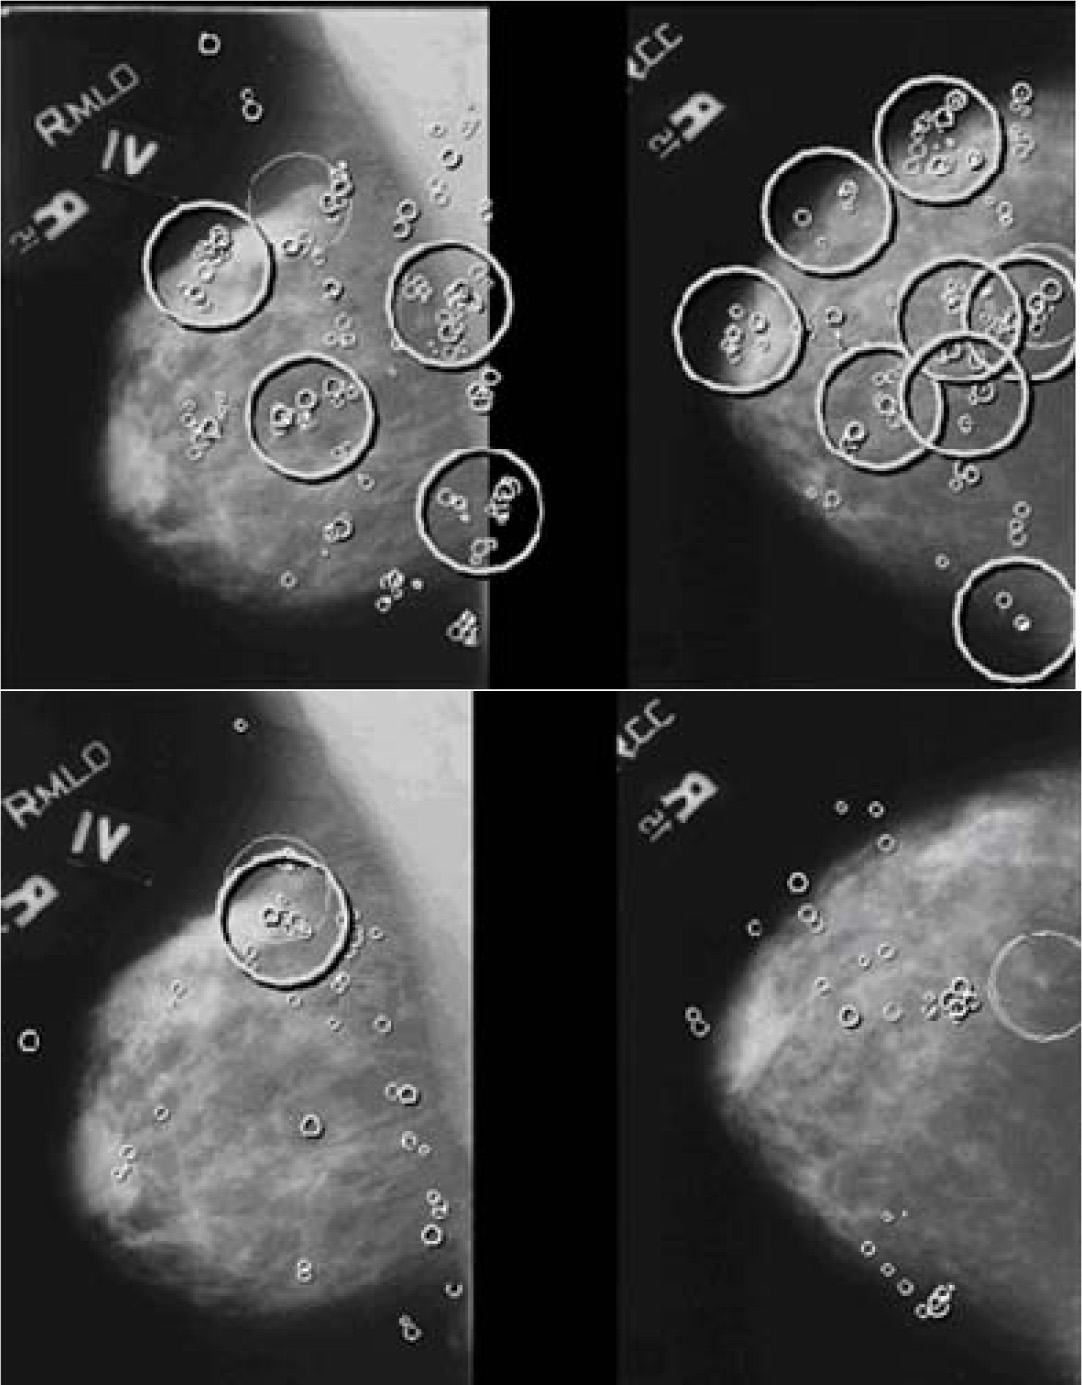
\includegraphics[width=300pt]{images/15-visual-search/eye-tracking-4-images} 

}

\caption{Eye-tracking recordings for a two-view digital mammogram. The top row is an inexperienced observer while the bottom row is an expert radiologist. The left column shows MLO views while the right column shows CC views.}\label{fig:visual-search-eye-tracking}
\end{figure}

\hypertarget{rsm}{%
\chapter{The radiological search model (RSM)}\label{rsm}}

\hypertarget{rsm-how-much-finished}{%
\section{How much finished}\label{rsm-how-much-finished}}

99\%

\hypertarget{rsm-intro}{%
\section{Introduction}\label{rsm-intro}}

All models of ROC data \emph{that do not incorporate search} involve two fundamental parameters (i.e., not including binning-related threshold parameters). For example, the unequal variance binormal model requires the \(a,b\) parameters. Alternative ROC models (e.g., CBM and PROPROC) also require two fundamental parameters.

Two fundamental parameters of ROC models are needed (1) to accommodate the average visibility of lesions in the dataset (e.g., the \(a\) or separation parameter) and (ii) the fact that the observed diseased case distribution is usually wider than that of the non-diseased cases (e.g., the \(b <1\) parameter). If one assumes same widths for both distributions, so in effect \(b=1\) is no longer a free parameter, and one allows a varying number of latent marks on all cases, then it becomes possible that the distribution of the highest rating on diseased cases will have greater width than that on non-diseased cases simply due to the fact that latent NLs on diseased cases will have lower z-samples than latent LLs on diseased cases (i.e., a mix of NL and LLs) while on non-diseased cases there will be only NL z-samples. So the basic idea is to have a visibility parameter, a parameter describing the distribution of the number of latent NLs per case and a parameter describing the distribution of the number of latent LLs per case, i.e., a three-parameter model should suffice. And in fact the RSM contains three fundamental parameters: \(\mu\), \(\lambda\) and \(\nu\). In addition the lowest threshold \(\zeta_1\) needs to be included as a parameter as it determines the extent and shape of the RSM predicted operating characteristics. This will become clearer in the next chapter but for now can be illustrated by considering the extreme case \(\zeta_1 = \infty\) when the predicted FROC is the single point (0,0).

\hypertarget{rsm-details}{%
\section{The radiological search model}\label{rsm-details}}

The radiological search model (RSM) for the free-response paradigm is a statistical parameterization of the Nodine-Kundel model. It consists of:

\begin{itemize}
\item
  A \emph{search stage} in which suspicious regions, i.e., the latent marks, are identified via peripheral vision. The total number of latent marks on a case is random non-negative integer and in fact some cases may have zero latent marks, a fact that will turn out to have important consequences for the shapes of all RSM predicted operating characteristics.
\item
  A \emph{decision stage} during which each latent mark is closely examined via foveal scanning, relevant features are extracted and analyzed and the observer calculates a decision variable or z-sample for each latent mark.
\item
  If the z-sample exceeds a pre-selected minimum reporting threshold, denoted \(\zeta_1\) the location is marked, i.e., the latent mark becomes an actual mark.
\item
  Latent marks can be either latent NLs (corresponding to non-diseased regions) or latent LLs (corresponding to lesions). The number of latent NLs or LLs on a case are denoted \(l_1, l_2\) respectively. Latent NLs can occur on non-diseased or diseased cases but latent LLs can only occur on diseased cases. Assume that every diseased case has \(L\) actual lesions (this will later be extended to arbitrary number of lesions per diseased case). \footnote{Since the RSM is a parametric model one does not need the four subscript notation needed to account for case and location dependence necessary to describe observed data, as in Chapter \ref{empirical}. This allows for simpler notation, as the reader may have noticed, unencumbered by 4 subscripts as in \(z_{k_ttl_ss}\) in Table \ref{empirical-notation}.}
\end{itemize}

\hypertarget{rsm-assumptions}{%
\section{RSM assumptions}\label{rsm-assumptions}}

\textbf{Assumption 1:} The number of latent NLs, \(l_1 \geq 0\), is sampled from the Poissson distribution \(\text{Pois}()\) with mean \(\lambda\):

\begin{equation} 
l_1 \sim \text{Pois}\left ( \lambda \right ) 
\label{eq:rsm-poisson-sampling}
\end{equation}

The probability mass function (pmf) of the Poissson distribution is defined by:

\begin{equation} 
\text{pmf}_{P}\left ( l_1, \lambda \right ) = exp\left ( -\lambda \right ) \frac{{(\lambda)^{l_1}}}{l_1!}
\label{eq:rsm-poisson-pmf}
\end{equation}

\textbf{Assumption 2:} The number of latent LLs, \(l_2\), where \(0 \leq l_2 \leq L\) (since the number of latent LLs cannot exceed the number of lesions) is sampled from the binomial distribution \(\text{B}\) with success probability \(\nu\) and trial size \(L\):

\begin{equation} 
l_2 \sim \text{B}\left ( L, \nu \right ) 
\label{eq:rsm-binomial-sampling}
\end{equation}

The probability mass function (pmf) of the binomial distribution is defined by:

\begin{equation} 
\text{pmf}_{B}\left ( l_2, L, \nu \right ) = \binom{L}{l_2} \left (\nu  \right )^{l_2} \left (1-\nu  \right )^{L-l_2}
\label{eq:rsm-binomial-pmf}
\end{equation}

\begin{quote}
Collectively \(\lambda\) and \(\nu\) are termed the \emph{search} parameters.
\end{quote}

\textbf{Assumption 3:} Each latent mark is associated with a z-sample. That for a latent NL is denoted \(z_{l_11}\) while that for a latent LL is denoted \(z_{l_22}\). Latent NLs can occur on non-diseased and diseased cases while latent LLs can only occur on diseased cases.

\textbf{Assumption 4:} For latent NLs the z-samples are obtained by sampling \(N \left ( 0, 1 \right )\):

\begin{equation} 
z_{l_11} \sim N \left ( 0, 1 \right )
\label{eq:rsm-sampling-l1}
\end{equation}

\textbf{Assumption 5:} For latent LLs the z-samples are obtained by sampling \(N \left ( \mu, 1 \right )\):

\begin{equation} 
z_{l_22} \sim N \left ( \mu, 1 \right )
\label{eq:rsm-sampling-l2}
\end{equation}

The probability density function \(\phi\left ( z | \mu \right )\) of the normal distribution \(N \left ( \mu, 1 \right )\) is defined by:

\begin{equation} 
\phi\left ( z | \mu \right )=\frac{1}{\sqrt{2\pi}}\exp\left ( -\frac{(z-\mu)^2}{2} \right )
\label{eq:rsm-pdf-phi-mu}
\end{equation}

\begin{quote}
The parameter \(\mu\) is termed the \emph{classification} parameter.
\end{quote}

\textbf{Bning rule:} In an FROC study with R ratings, the observer adopts \(R\) ordered cutoffs \(\zeta_r\), where \(\left ( r = 1, 2, ..., R \right )\). Defining \(\zeta_0 = -\infty\) and \(\zeta_{R+1} = \infty\), then if \(\zeta_r \leq z_{l_ss} < \zeta_{r+1}\) the corresponding latent site is marked and rated in bin \(r\), and if \(z_{l_ss} \leq \zeta_1\) the site is not marked. (\(R\) is the number of FROC bins.)

\textbf{Mark location:} The location of the mark is assumed to be at the exact center of the latent site that exceeded a cutoff and an infinitely precise proximity criterion is adopted. Consequently, there is no confusing a mark made because of a latent LL z-sample exceeding the cutoff with one made because of a latent NL z-sample exceeding the cutoff. Therefore, any mark made because of a latent NL z-sample that satisfies \(\zeta_r \leq z_{l_11} < \zeta_{r+1}\) will be scored as a non-lesion localization (NL) and rated \(r\). Likewise, any mark made because of a latent LL z-sample that satisfies \(\zeta_r \leq z_{l_22} < \zeta_{r+1}\) will be scored as a lesion-localization (LL) and rated \(r\).

\textbf{Rating assigned to unmarked sites:} Unmarked LLs are assigned the zero rating (or any rating lower than the lowest allowed FROC-1 rating). Note that even lesions that were not found by the search stage, and therefore do not qualify as latent LLs, are assigned the zero rating. This is because they represent observable events (and less suspicious than the lowest allowed FROC-1 rating). In contrast, unmarked latent NLs are unobservable events. Unlike lesions there is no a-priori reader-independent list of non-lesion locations; what constitutes a NL is reader dependent, see Fig. \ref{fig:visual-search-eye-tracking}.

By choosing \(R\) large enough the preceding discrete rating model is applicable to quasi-continuous z-samples.

\hypertarget{rsm-parameter-physical-meanings}{%
\section{Physical meanings of the RSM parameters}\label{rsm-parameter-physical-meanings}}

The parameters have the following physical meanings:

\hypertarget{rsm-mu-parameter}{%
\subsection{\texorpdfstring{The \(\mu\) parameter}{The \textbackslash mu parameter}}\label{rsm-mu-parameter}}

The \(\mu\) parameter is the lesion \emph{perceptual signal to noise ratio pSNR}, as described in (print book) Chapter 12.5.2, between latent NLs and latent LLs. For white noise background this is similar to the physical SNR \citep{chakraborty1997computer} after correction for the non-linear response of the visual system to visual stimuli \citep{siddiqui2005discrete}. For clinical backgrounds pSNR is determined by the competition for the observer's foveal attention from other regions that could be mistaken for lesions.

The \(\mu\) parameter is similar to detectability index \(d'\), which is the separation parameter of two unit normal distributions required to achieve the observed probability of correct choice (PC) in a two alternative forced choice task between cued NLs and cued LLs. Individually and for each reader one determines the locations of the latent marks using eye-tracking apparatus and then runs a 2AFC study as follows: pairs of images are shown, each with a cued location, one a latent NL and the other a latent LL, where all locations were recorded in prior eye-tracking sessions for the specific radiologist. The radiologist's task is to pick the image with the latent LL. The probability correct \(\text{PC}\) in this task is related to the \(\mu\) parameter by:

\begin{equation} 
\mu = \sqrt{2} \Phi^{-1} \left ( \text{PC} \right )
\label{eq:rsm-mu-2afc}
\end{equation}

The radiologist on whom the eye-tracking measurements are performed and the one who performs the two alternative forced choice tasks must be the same, as two radiologists may not agree on latent NL marks. A complication in conducting such a study is that because of memory effects a lesion can only be shown once to each reader: clinical images are distinctive - once a radiologist has found a lesion in a clinical image, that event may become imprinted in long-term memory; one cannot repeatedly compare this lesion to other NLs in the 2AFC task as the radiologist will always pick the remembered lesion. This is a difficult study to conduct as I found out.

\hypertarget{rsm-summary-lambda-parameter}{%
\subsection{\texorpdfstring{The \(\lambda\) parameter}{The \textbackslash lambda parameter}}\label{rsm-summary-lambda-parameter}}

The \(\lambda\) parameter determines the tendency of the observer to generate latent NLs. The mean number of latent NLs per case is an estimate of \(\lambda\). \footnote{It can be measured via eye-tracking apparatus. This time it is only necessary to cluster the marks and classify each mark as a latent NL or latent LL according to the adopted acceptance radius. An eye-tracking based estimate would be the total number of latent NLs in the dataset divided by the total number of cases.}

I have found it best to illustrate sampling to non-statistics majors with numerical examples. Consider two observers, one with \(\lambda = 1\) and the other with \(\lambda = 2\). While one cannot predict the exact number of latent NLs on any specific case, the value of \(\lambda\) determines the average number of latent NLs.

The following code illustrates Poissson sampling, estimation of the mean and confidence interval for 100 samples from two Poissson distributions. The number of samples has been set to \(K_1=100\) (the first argument to \texttt{rpois()} is the number of non-diseased cases; the second argument is the value of \(\lambda\)).

\begin{Shaded}
\begin{Highlighting}[]
\NormalTok{K1 }\OtherTok{\textless{}{-}} \DecValTok{100}
\NormalTok{lambda }\OtherTok{\textless{}{-}} \FunctionTok{c}\NormalTok{(}\DecValTok{1}\NormalTok{,}\DecValTok{2}\NormalTok{)}
\NormalTok{seed }\OtherTok{\textless{}{-}} \DecValTok{1}\NormalTok{;}\FunctionTok{set.seed}\NormalTok{(seed);samples1 }\OtherTok{\textless{}{-}} \FunctionTok{rpois}\NormalTok{(K1,}\AttributeTok{lambda =}\NormalTok{ lambda[}\DecValTok{1}\NormalTok{])}
\NormalTok{seed }\OtherTok{\textless{}{-}} \DecValTok{1}\NormalTok{;}\FunctionTok{set.seed}\NormalTok{(seed);samples2 }\OtherTok{\textless{}{-}} \FunctionTok{rpois}\NormalTok{(K1,}\AttributeTok{lambda =}\NormalTok{ lambda[}\DecValTok{2}\NormalTok{])}

\NormalTok{ret11 }\OtherTok{\textless{}{-}} \FunctionTok{poisson.exact}\NormalTok{(}\FunctionTok{sum}\NormalTok{(samples1),K1)}
\NormalTok{ret21 }\OtherTok{\textless{}{-}} \FunctionTok{poisson.exact}\NormalTok{(}\FunctionTok{sum}\NormalTok{(samples2),K1)}
\end{Highlighting}
\end{Shaded}

\begin{verbatim}
## K1 =  100 , lambda 1st reader =  1 , lambda 2nd reader =  2
\end{verbatim}

\begin{verbatim}
## obs. mean, reader 1 =  1.01
\end{verbatim}

\begin{verbatim}
## obs. mean, reader 2 =  2.02
\end{verbatim}

\begin{verbatim}
## Rdr. 1: 95% CI =  [ 0.8226616 1.227242 ]
\end{verbatim}

\begin{verbatim}
## Rdr. 2: 95% CI =  [ 1.751026 2.318599 ]
\end{verbatim}

For reader 1 the estimate of the Poissson parameter (the mean parameter of the Poissson distribution is frequently referred to as the Poissson parameter) is 1.01 with 95\% confidence interval (0.823, 1.227); for reader 2 the corresponding estimates are 2.02 and (1.751, 2.319). As the number of cases increases, the confidence interval shrinks. For example, with 10000 cases, i.e., 100 times the value in the previous example:

\begin{verbatim}
## K1 =  10000 , lambda 1st reader =  1 , lambda 2nd reader =  2
\end{verbatim}

\begin{verbatim}
## obs. mean, reader 1 =  1.0055
\end{verbatim}

\begin{verbatim}
## obs. mean, reader 2 =  2.006
\end{verbatim}

\begin{verbatim}
## Rdr. 1: 95% CI =  [ 0.9859414 1.025349 ]
\end{verbatim}

\begin{verbatim}
## Rdr. 2: 95% CI =  [ 1.978335 2.033955 ]
\end{verbatim}

This time for reader 1, the estimate of the Poissson parameter is 1.01 with 95\% confidence interval (0.986, 1.025); for reader 2 the corresponding estimate is 2.01 with 95\% confidence interval (1.978, 2.034). The width of the confidence interval is inversely proportional to the square root of the number of cases (the example below is for reader 1):

\begin{Shaded}
\begin{Highlighting}[]
\NormalTok{ret11}\SpecialCharTok{$}\NormalTok{conf.int[}\DecValTok{2}\NormalTok{] }\SpecialCharTok{{-}}\NormalTok{ ret11}\SpecialCharTok{$}\NormalTok{conf.int[}\DecValTok{1}\NormalTok{]}
\end{Highlighting}
\end{Shaded}

\begin{verbatim}
## [1] 0.40458
\end{verbatim}

\begin{Shaded}
\begin{Highlighting}[]
\NormalTok{ret12}\SpecialCharTok{$}\NormalTok{conf.int[}\DecValTok{2}\NormalTok{] }\SpecialCharTok{{-}}\NormalTok{ ret12}\SpecialCharTok{$}\NormalTok{conf.int[}\DecValTok{1}\NormalTok{]}
\end{Highlighting}
\end{Shaded}

\begin{verbatim}
## [1] 0.03940756
\end{verbatim}

Since the number of cases was increased by a factor of 100, the width decreased by a factor of 10, the square-root of the ratio of the numbers of cases.

\hypertarget{rsm-summary-nu-parameter}{%
\subsection{\texorpdfstring{The \(\nu\) parameter}{The \textbackslash nu parameter}}\label{rsm-summary-nu-parameter}}

The \(\nu\) parameter determines the ability of the observer to find lesions. Assuming the same number of lesions per diseased case, the fraction of latent LLs per diseased case is an estimate of \(\nu\). \footnote{It too can be measured via eye-tracking apparatus performed on a radiologist. An eye-tracking based estimate would be the total number of latent LLs in the dataset divided by the total number of lesions.}

Consider two observers, one with \(\nu = 0.5\) and the other with \(\nu = 0.9\). Again, while one cannot predict the number of latent LLs on any specific diseased case, or which lesions will be correctly localized, one can predict the average number of latent LLs per diseased case.

The following code uses \(K_2 = 100\) samples, the number of diseased cases, each with one lesion. The arguments to \texttt{rbinom()} - for random binomial samples - are the number of diseased cases, the number of lesions per case and the value of \(\nu\).

\begin{Shaded}
\begin{Highlighting}[]
\NormalTok{K2 }\OtherTok{\textless{}{-}} \DecValTok{100}
\NormalTok{nu }\OtherTok{\textless{}{-}} \FunctionTok{c}\NormalTok{(}\FloatTok{0.5}\NormalTok{, }\FloatTok{0.9}\NormalTok{)}
\NormalTok{seed }\OtherTok{\textless{}{-}} \DecValTok{1}\NormalTok{;}\FunctionTok{set.seed}\NormalTok{(seed);samples1 }\OtherTok{\textless{}{-}} \FunctionTok{rbinom}\NormalTok{(K2,}\DecValTok{1}\NormalTok{,nu[}\DecValTok{1}\NormalTok{])}
\NormalTok{seed }\OtherTok{\textless{}{-}} \DecValTok{1}\NormalTok{;}\FunctionTok{set.seed}\NormalTok{(seed);samples2 }\OtherTok{\textless{}{-}} \FunctionTok{rbinom}\NormalTok{(K2,}\DecValTok{1}\NormalTok{,nu[}\DecValTok{2}\NormalTok{])}

\NormalTok{ret1 }\OtherTok{\textless{}{-}} \FunctionTok{binom.exact}\NormalTok{(}\FunctionTok{sum}\NormalTok{(samples1),K2)}
\NormalTok{ret2 }\OtherTok{\textless{}{-}} \FunctionTok{binom.exact}\NormalTok{(}\FunctionTok{sum}\NormalTok{(samples2),K2)}
\end{Highlighting}
\end{Shaded}

\begin{verbatim}
## K2 =  100 , nu 1st reader =  0.5 , nu 2nd reader =  0.9
\end{verbatim}

\begin{verbatim}
## mean, reader 1 =  0.48
\end{verbatim}

\begin{verbatim}
## mean, reader 2 =  0.94
\end{verbatim}

\begin{verbatim}
## Rdr. 1: 95% CI =  [ 0.3790055 0.5822102 ]
\end{verbatim}

\begin{verbatim}
## Rdr. 2: 95% CI =  [ 0.8739701 0.9776651 ]
\end{verbatim}

The result shows that for reader 1 the estimate of the binomial success rate parameter is 0.48 with 95\% confidence interval (0.379, 0.582). For reader 2 the corresponding estimates are 0.94 and (0.874, 0.978).

As a more complicated but clinically realistic example, consider a dataset with 100 cases where 97 cases have one lesion per case, two have two lesions per case and one has three lesions per case (these are typical lesion distributions observed in screening mammography). The code follows:

\begin{Shaded}
\begin{Highlighting}[]
\NormalTok{K2 }\OtherTok{\textless{}{-}} \FunctionTok{c}\NormalTok{(}\DecValTok{97}\NormalTok{,}\DecValTok{2}\NormalTok{,}\DecValTok{1}\NormalTok{);Lk }\OtherTok{\textless{}{-}} \FunctionTok{c}\NormalTok{(}\DecValTok{1}\NormalTok{,}\DecValTok{2}\NormalTok{,}\DecValTok{3}\NormalTok{);nu }\OtherTok{\textless{}{-}} \FunctionTok{c}\NormalTok{(}\FloatTok{0.5}\NormalTok{, }\FloatTok{0.9}\NormalTok{)}
\NormalTok{samples1 }\OtherTok{\textless{}{-}} \FunctionTok{array}\NormalTok{(}\AttributeTok{dim =} \FunctionTok{c}\NormalTok{(}\FunctionTok{sum}\NormalTok{(K2),}\FunctionTok{length}\NormalTok{(K2)))}
\NormalTok{seed }\OtherTok{\textless{}{-}} \DecValTok{1}\NormalTok{;}\FunctionTok{set.seed}\NormalTok{(seed)}
\CommentTok{\# I am using el instead of l as the latter looks like 1}
\ControlFlowTok{for}\NormalTok{ (el }\ControlFlowTok{in} \DecValTok{1}\SpecialCharTok{:}\FunctionTok{length}\NormalTok{(K2)) \{}
\NormalTok{  samples1[}\DecValTok{1}\SpecialCharTok{:}\NormalTok{K2[el],el] }\OtherTok{\textless{}{-}} \FunctionTok{rbinom}\NormalTok{(K2[el],Lk[el],nu[}\DecValTok{1}\NormalTok{])}
\NormalTok{\}}

\NormalTok{samples2 }\OtherTok{\textless{}{-}} \FunctionTok{array}\NormalTok{(}\AttributeTok{dim =} \FunctionTok{c}\NormalTok{(}\FunctionTok{sum}\NormalTok{(K2),}\FunctionTok{length}\NormalTok{(K2)))}
\NormalTok{seed }\OtherTok{\textless{}{-}} \DecValTok{1}\NormalTok{;}\FunctionTok{set.seed}\NormalTok{(seed)}
\ControlFlowTok{for}\NormalTok{ (el }\ControlFlowTok{in} \DecValTok{1}\SpecialCharTok{:}\FunctionTok{length}\NormalTok{(K2)) \{}
\NormalTok{  samples2[}\DecValTok{1}\SpecialCharTok{:}\NormalTok{K2[el],el] }\OtherTok{\textless{}{-}} \FunctionTok{rbinom}\NormalTok{(K2[el],Lk[el],nu[}\DecValTok{2}\NormalTok{])}
\NormalTok{\}}

\NormalTok{ret1 }\OtherTok{\textless{}{-}} \FunctionTok{binom.exact}\NormalTok{(}\FunctionTok{sum}\NormalTok{(samples1[}\SpecialCharTok{!}\FunctionTok{is.na}\NormalTok{(samples1)]),}\FunctionTok{sum}\NormalTok{(K2}\SpecialCharTok{*}\NormalTok{Lk))}
\NormalTok{ret2 }\OtherTok{\textless{}{-}} \FunctionTok{binom.exact}\NormalTok{(}\FunctionTok{sum}\NormalTok{(samples2[}\SpecialCharTok{!}\FunctionTok{is.na}\NormalTok{(samples2)]),}\FunctionTok{sum}\NormalTok{(K2}\SpecialCharTok{*}\NormalTok{Lk))}
\end{Highlighting}
\end{Shaded}

\begin{verbatim}
## K2[1] = 97 , K2[2] = 2 , K2[3] = 1 , nu1 = 0.5 , nu2 = 0.9
\end{verbatim}

\begin{verbatim}
## obsvd. mean, reader 1 =  0.4903846
\end{verbatim}

\begin{verbatim}
## obsvd. mean, reader 2 =  0.9326923
\end{verbatim}

\begin{verbatim}
## Rdr. 1: 95% CI =  0.3910217 0.5903092
\end{verbatim}

\begin{verbatim}
## Rdr. 2: 95% CI =  0.8662286 0.9725125
\end{verbatim}

For reader 1, the estimate of the binomial success probability is 0.490 with 95\% confidence interval (0.391, 0.590); for reader 2 the corresponding estimates are 0.933 and (0.866, 0.973).

\hypertarget{rsm-intrinsic-parameters}{%
\section{Intrinsic RSM parameters}\label{rsm-intrinsic-parameters}}

While the parameters \(\lambda\) and \(\nu\) are physically meaningful a little thought reveals that they must depend on \(\mu\). From the solar-analogy described in Section \ref{froc-paradigm-solar-analogy} we know that if \(\mu = 0\) the lesions have zero contrast and therefore cannot be found by the search mechanism implying \(\nu = 0\). Moreover attempting to find these zero contrast lesions must generate a large number of non-lesion localizations implying \(\lambda = \infty\).

The following is a simple model of the \(\mu\) dependence of \(\lambda\) and \(\nu\). The model re-parameterizes the \emph{physical} parameters \(\lambda\) and \(\nu\) in terms of \emph{intrinsic} parameters \(\lambda_i\) and \(\nu_i\) that are \(\mu\) independent\footnote{The need for the first re-parameterization, involving \(\nu\), was foreseen in the original search model papers \citep{chakraborty2006search, chakraborty2006roc} but the need for the second re-parameterization (involving \(\lambda\)) became evident more recently.}:

\begin{equation}
\left. 
\begin{aligned}
\nu =& 1 - \text{exp}\left ( - \mu \nu_i \right ) \\
\lambda =& \frac{\lambda_i}{\mu}
\end{aligned}
\right \}
\label{eq:rsm-transform}
\end{equation}

The inverse transformations are:

\begin{equation}
\left. 
\begin{aligned}
\nu_i =& - \frac{\ln \left ( 1-\nu \right )}{\mu}\\
\lambda_i =& \mu \lambda 
\end{aligned}
\right \}
\label{eq:rsm-inv-transform}
\end{equation}

The intrinsic parameters obey \(\lambda_i \ge 0\) and \(\nu_i \ge 0\).

Since it determines \(\nu\), the \(\nu_i\) parameter can be considered as the intrinsic (i.e., \(\mu\)-independent) ability to find lesions; specifically, \emph{it is the rate of increase of \(\nu\) with \(\mu\) at small \(\mu\)}:

\begin{equation} 
\nu_i = \left (\frac{\partial \nu}{\partial \mu}  \right )_{\mu = 0}
\label{eq:rsm-nup-limit}
\end{equation}

According to Eqn. \eqref{eq:rsm-transform}, as \(\mu \rightarrow \infty\), \(\nu \rightarrow 1\) and conversely, as \(\mu \rightarrow 0\), \(\nu \rightarrow 0\). The solar analogy in Section \ref{froc-paradigm-solar-analogy} is instructive. The dependence of \(\nu\) on \(\mu\) is consistent with the fact that higher contrast lesions are easier to find. A non-expert is expected to find a high contrast lesion whereas a low contrast lesion will be more difficult to find even by an expert observer.

According to Eqn. \eqref{eq:rsm-transform} the value of \(\mu\) also determines \(\lambda\): as \(\mu \rightarrow \infty\), \(\lambda \rightarrow 0\), and conversely, as \(\mu \rightarrow 0\), \(\lambda \rightarrow \infty\). Here too the solar analogy in Section \ref{froc-paradigm-solar-analogy} is instructive. Since the sun has very high contrast, there is no reason for the observer to search for other suspicious regions which have no possibility of resembling it. On the other hand, attempting to locate a faint star can generate many false sightings because the expected small contrast from the faint real star could be comparable to that from a number of regions in the nearby background.

\hypertarget{rsm-discussion-summary}{%
\section{Summary}\label{rsm-discussion-summary}}

This chapter has described a statistical parameterization of the Nodine-Kundel model of visual search. The model accounts for key aspects of the process:

\begin{itemize}
\tightlist
\item
  Search: finding lesions and finding non-lesions. These are characterized by the two search parameters \(\lambda\) and \(\nu\).
\item
  Classification: The ability to correctly rate a lesion higher than a NL is characterized by the third (classification) parameter of the model \(\mu\).
\end{itemize}

While the 2 search parameters have relatively simple physical meanings they depend on \(\mu\). Consequently, it is necessary to introduce intrinsic parameters \(\lambda_i\) and \(\nu_i\) which are independent of \(\mu\).

The next chapter explores the ROC curve predictions of the radiological search model.

\hypertarget{rsm-predictions}{%
\chapter{ROC predictions of the RSM}\label{rsm-predictions}}

\hypertarget{rsm-predictions-how-much-finished}{%
\section{TBA How much finished}\label{rsm-predictions-how-much-finished}}

90\%

\hypertarget{rsm-predictions-intro}{%
\section{TBA Introduction}\label{rsm-predictions-intro}}

The preceding chapter described the radiological search model (RSM) for FROC data. This chapter describes ROC-related predictions of the RSM. The next chapter will describe the FROC, AFROC and wAFROC curve predictions.

The inferred-ROC z-sample and the end-point of the ROC are defined and expressions in terms of RSM parameters are derived. Derived next is the predicted \emph{inferred ROC} curve and the probability density functions of the inferred-ROC z-samples for non-diseased and diseased cases. Integrating the total area under the predicted ROC yields ROC-AUC.

Since the ROC is a basic measure of performance, numerical examples are given showing the behavior of the operating point as parameters of the RSM are varied.

In this chapter formulae for RSM quantities are given in terms of the RSM search parameters \(\lambda\) and \(\nu\).

\hypertarget{rsm-predictions-inferred-roc}{%
\section{Inferred ROC z-sample}\label{rsm-predictions-inferred-roc}}

\emph{The inferred ROC z-sample of a case, denoted \(h_t\), where \(t = 1\) for non-diseased cases and \(t = 2\) for diseased cases, is the z-sample of the highest rated latent mark on the case or \(-\infty\) if the case has no latent marks.} The difference from the previous chapter is that in this chapter we are concerned with statistical/probabilistic modeling of the continuous z-samples instead of describing observed ratings for a finite dataset.

Definitions:

\begin{quote}
\begin{itemize}
\tightlist
\item
  \(\text{FPF}(\zeta)\) = probability that \(h_1 \ge \zeta\).
\item
  \(\text{TPF}(\zeta)\) = probability that \(h_2 \ge \zeta\).
\end{itemize}
\end{quote}

Accordingly, FPF and TPF are defined by:

\begin{equation}
\text{FPF}\left( \zeta \right) = \text{P} \left ( h_1 \geq \zeta\right )
\label{eq:rsm-predictions-fpf-def}
\end{equation}

\begin{equation}
\text{TPF}\left( \zeta \right) = \text{P} \left ( h_2 \geq \zeta\right )
\label{eq:rsm-predictions-tpf-def}
\end{equation}

Definition of ROC plot:

\begin{quote}
\begin{itemize}
\tightlist
\item
  The ROC is the plot of \(\text{TPF}(\zeta)\) vs.~\(\text{FPF}(\zeta)\).
\item
  \emph{The plot includes a straight line extension from the theoretical end-point to (1,1)}.
\item
  The theoretical end-point corresponds to \(\zeta = -\infty\).
\end{itemize}
\end{quote}

\hypertarget{rsm-predictions-end-point}{%
\section{End-point of the ROC}\label{rsm-predictions-end-point}}

A consequence of the possibility that some cases have no marks is that the ROC curve has the \emph{end-point-discontinuity property}, namely the full range of ROC space, i.e., \(0 \leq \text{FPF} \leq 1\) and \(0 \leq \text{TPF} \leq 1\), is not continuously accessible to the observer. In fact, \(0 \leq \text{FPF} \leq \text{FPF}_{\text{max}}\) and \(0 \leq \text{TPF} \leq \text{TPF}_{\text{max}}\) where \(\text{FPF}_{\text{max}}\) and \(\text{TPF}_{\text{max}}\) are generally less than unity.

Starting from \(\infty\) as \(\zeta\) is lowered to \(-\infty\) some of the cases that had at least one latent site but whose z-sample did not exceed \(\zeta\) will now generate marks and contribute to \(\text{FPF}\) and \(\text{TPF}\) resulting in upward and rightward movement of the theoretical operating point until eventually \emph{only cases with no latent sites} remain. These cases cannot generate marks. The finite number of cases with no marks has the consequence that the uppermost continuously accessible operating point is below-left of (1,1). The (1,1) point is ``trivially'' reached when one cumulates cases with no marks, i.e., those rated \(-\infty\).

This behavior is distinct from conventional ROC models where the entire curve, extending from (0, 0) to (1, 1), is continuously accessible. This is because every case yields a finite decision variable, no matter how small. The number of cases with \(-\infty\) rating is zero. When \(\zeta = -\infty\) the operating point reaches (1,1).

\hypertarget{rsm-predictions-constrained-end-point-abscissa}{%
\subsection{The abscissa of the ROC end-point}\label{rsm-predictions-constrained-end-point-abscissa}}

Consider the probability that a non-diseased case has at least one latent NL. Such a case will generate a finite value of \(h_1\) and with an appropriately low \(\zeta\) it will be marked. The probability of \emph{zero} latent NLs, see Eqn. \eqref{eq:rsm-poisson-pmf}, is:

\[\text{pmf}_{P} \left (0,\lambda \right ) = \text{exp} \left ( -\lambda \right )\].

The probability that the case has \emph{at least one} latent NL is the complement of the above probability. At sufficiently low \(\zeta\) each of these cases yields a marked non-disease case. Therefore, the maximum continuously accessible abscissa of the ROC, i.e., \(\text{FPF}_{\text{max}}\), is:

\begin{equation} 
\text{FPF}_{\text{max}} = 1 - \text{exp} \left ( -\lambda \right )
\label{eq:rsm-predictions-fpf-max}
\end{equation}

\hypertarget{rsm-predictions-constrained-end-point-ordinate}{%
\subsection{The ordinate of the ROC end-point}\label{rsm-predictions-constrained-end-point-ordinate}}

A diseased case has no marks, even for very low \(\zeta\), if it has zero latent NLs, the probability of which is \(\text{exp}(-\lambda)\), and it has zero latent LLs, the probability of which is, see Eqn. \eqref{eq:rsm-binomial-pmf}, \(\text{pmf}_{B} \left ( 0, L, \nu \right )= (1 - \nu)^L\).

Here \(L\) is the number of lesions in each diseased case.

\begin{itemize}
\item
  Assumption 1: occurrences of latent LLs are independent of each other, i.e., the probability that a lesion is found is independent of whether other lesions are found on the same case.
\item
  Assumption 2: occurrences of latent NLs are independent of each other; i.e., the probability of a NL is independent of whether other NLs are found on the same case.
\item
  Assumption 3: occurrence of a latent NL is independent of the occurrence of a latent LL on the same case.
\end{itemize}

By these assumptions the probability of zero latent NLs \emph{and} zero latent LLs on a diseased case is the product of the two probabilities, namely

\[\text{exp}(-\lambda) (1 - \nu)^L\].

The probability that there exists \emph{at least one} latent site is the complement of the above expression, which equals \(\text{TPF}_{\text{max}}\), i.e.,

\begin{equation}
\text{TPF}_{\text{max}} = 1 - \text{exp} \left ( - \lambda \right ) \left ( 1 - \nu \right )^L
\label{eq:rsm-predictions-tpf-max}
\end{equation}

\hypertarget{rsm-predictions-end-point-variable-number-lesions}{%
\subsection{Variable number of lesions per case}\label{rsm-predictions-end-point-variable-number-lesions}}

Defining \(f_L\) the fraction of diseased cases with \(L\) lesions and \(L_{max}\) the maximum number of lesions per diseased case in the dataset, then:

\begin{equation}
\sum_{L=1}^{{L_{max}}}  f_L = 1
\label{eq:rsm-predictions-fl-sum}
\end{equation}

By restricting attention to the set of diseased cases with \(L\) lesions each, Eqn. \eqref{eq:rsm-predictions-tpf-max} for \(\text{TPF}_{\text{max}}\) applies. Since TPF is a probability and probabilities of independent processes add it follows that:

\begin{equation}
\text{TPF}_{\text{max}} = 1 - \text{exp} \left ( - \lambda \right ) \sum_{L=1}^{L_{max}}f_L \left ( 1 - \nu \right )^L
\label{eq:rsm-predictions-tpf-max-vary-l}
\end{equation}

The ordinate of the end-point is a \(f_L\) weighted summation of \(\text{TPF}_{\text{max}}\). The expression for \(\text{FPF}_{\text{max}}\) is unaffected.

\hypertarget{rsm-predictions-roc-curve}{%
\section{ROC curve}\label{rsm-predictions-roc-curve}}

On the continuous ROC curve each case has at least one mark and the ROC decision variable is the rating of the highest rated mark \(h_t\) on the case. Therefore Eqn. \eqref{eq:rsm-predictions-fpf-def} and Eqn. \eqref{eq:rsm-predictions-tpf-def} apply. Varying the threshold parameter \(\zeta\) from \(\infty\) to \(-\infty\) sweeps out the continuous section of the predicted ROC curve from (0,0) to \(\left (\text{FPF}_{\text{max}}, \text{TPF}_{\text{max}} \right )\).

\hypertarget{rsm-predictions-roc-curve-fpf}{%
\subsection{Derivation of FPF}\label{rsm-predictions-roc-curve-fpf}}

\begin{itemize}
\tightlist
\item
  Assumption 4: the z-samples of latent NLs on the same case are independent of each other.
\end{itemize}

Consider the set of non-diseased cases with \(n\) latent NLs each, where \(n > 0\). According to \ref{rsm-assumptions} each latent NL yields a z sample from \(N(0,1)\). The probability that a z-sample from a latent NL is smaller than \(\zeta\) is \(\Phi(\zeta)\). The probability that all \(n\) z-samples are smaller than \(\zeta\) is \((\Phi(\zeta))^n\). If all z-samples are smaller than \(\zeta\), then the highest z-sample \(h_t\) must be smaller than \(\zeta\). Therefore, the probability that \(h_t\) exceeds \(\zeta\) is:

\begin{equation}
\left. 
\begin{aligned}
\text{FPF}\left (\zeta \mid n \right ) =& P\left ( h_1 \geq  \zeta \mid n\right ) \\
=& 1 - \left [ \Phi\left ( \zeta \right )  \right ]^n
\end{aligned}
\right \}
\label{eq:rsm-predictions-fpf-zeta-n}
\end{equation}

The conditioning notation in Eqn. \eqref{eq:rsm-predictions-fpf-zeta-n} reflects the fact that this expression applies specifically to non-diseased cases each with \(n\) latent NLs. To obtain \(\text{FPF}_{\text{max}}\) one performs a Poissson pmf-weighted summation of \(\text{FPF}\left (\zeta \mid n \right )\) over \(n\) from 0 to \(\infty\) (the inclusion of the \(n = 0\) term is explained below):

\begin{equation}
\text{FPF}\left (\zeta, \lambda \right ) = \sum_{n=0}^{\infty} \text{pmf}_{\text{Pois}} \left ( n, \lambda \right )\text{FPF}\left (\zeta \mid n \right )
\label{eq:rsm-predictions-fpf-zeta-before-maple}
\end{equation}

The infinite summations, see below, are easier performed using symbolic algebra software such as \(\text{Maple}^{TM}\). Inclusion in the summation of \(n = 0\), which evaluates to zero, is done to make it easier for \(\text{Maple}^{TM}\) to evaluate the summation in closed form. Otherwise one may need to simplify the \(\text{Maple}^{TM}\)-generated result. The \(\text{Maple}^{TM}\) code is shown below (Maple 17, Waterloo Maple Inc.).

\begin{verbatim}
# Maple Code
restart;
phi := proc (t, mu) exp(-(1/2)*(t-mu)^2)/sqrt(2*Pi) end: 
PHI := proc (c, mu) local t; int(phi(t, mu), t = -infinity .. c) end: 
Poissson := proc (n, lambda) lambda^n*exp(-lambda)/factorial(n) end: 
B := proc (l, L, nu) binomial(L, l)*nu^l*(1-nu)^(L-l) end:
FPF := proc(zeta,lambda) sum(Poissson(n,lambda)*
(1 - PHI(zeta,0)^n), n=0..infinity);end:
FPF(zeta, lambda);   
\end{verbatim}

The above code yields:

\begin{equation}
\text{FPF}\left (\zeta , \lambda\right ) = 1 - \text{exp}\left ( -\frac{\lambda}{2} \left [ 1-\text{erf}\left ( \frac{\zeta}{\sqrt{2}} \right ) \right ]  \right ) 
\label{eq:rsm-predictions-fpf-erf}
\end{equation}

The error function in Eqn. \eqref{eq:rsm-predictions-fpf-erf} is related to the unit normal CDF function \(\Phi(x)\) by:

\begin{equation}
\text{erf} \left (x \right ) =  2\Phi \left ( \sqrt{2} x\right ) - 1
\label{eq:rsm-predictions-erf-phi-relation}
\end{equation}

Using this transformation yields the following simpler expression for FPF:

\begin{equation}
\text{FPF}\left (\zeta , \lambda\right ) = 1 - \text{exp}\left ( -\lambda \Phi\left ( -\zeta \right )  \right )
\label{eq:rsm-predictions-fpf}
\end{equation}

The \texttt{R} implementation follows:

\begin{Shaded}
\begin{Highlighting}[]
\CommentTok{\# lambda is the physical lambda\textquotesingle{} parameter}
\NormalTok{FPF }\OtherTok{\textless{}{-}} \ControlFlowTok{function}\NormalTok{ (zeta, lambda) \{}
\NormalTok{  x }\OtherTok{=} \DecValTok{1} \SpecialCharTok{{-}} \FunctionTok{exp}\NormalTok{(}\SpecialCharTok{{-}}\NormalTok{lambda }\SpecialCharTok{*} \FunctionTok{pnorm}\NormalTok{(}\SpecialCharTok{{-}}\NormalTok{zeta))}
  \FunctionTok{return}\NormalTok{(x)}
\NormalTok{\}}
\end{Highlighting}
\end{Shaded}

Because \(\Phi\) ranges from 0 to 1, \(\text{FPF}\left (\zeta , \lambda\right )\) ranges from 0 to \(\text{exp} \left ( -\lambda \right )\).

\hypertarget{rsm-predictions-roc-curve-tpf}{%
\subsection{Derivation of TPF}\label{rsm-predictions-roc-curve-tpf}}

The derivation of the true positive fraction \(\text{TPF}(\zeta)\) follows a similar line of reasoning except this time one needs to consider the highest of the latent NLs and latent LL z-samples. Consider a diseased case with L lesions, \(n\) latent NLs and \(l\) latent LLs. Each latent NL yields a decision variable sample from \(N(0,1)\) and each latent LL yields a sample from \(N(\mu,1)\). The probability that all \(n\) latent NLs have z-samples less than \(\zeta\) is \([\Phi(\zeta)]^n\). The probability that all \(l\) latent LLs have z-samples less than \(\zeta\) is \([\Phi(\zeta - \mu)]^l\). The probability that all latent marks have z-samples less than \(\zeta\) is the product of these two probabilities. The probability that \(h_2\) (the highest z-sample on a diseased case) is larger than \(\zeta\) is the complement of the product probabilities, i.e.,

\begin{equation}
\left. 
\begin{aligned}
\text{TPF}\left ( \zeta, \mu, n, l, L \right ) =& 
P\left ( h_2 \geq \zeta \mid \mu, n, l, L \right ) \\
=& 1 - \left [ \Phi\left ( \zeta \right ) \right ]^n \left [ \Phi\left ( \zeta - \mu\right ) \right ]^l
\end{aligned}
\right \}
\label{eq:rsm-predictions-tpf-vary-nl}
\end{equation}

One averages over the distributions of \(n\) and \(l\) to obtain the desired ROC-ordinate:

\begin{equation}
\left.
\begin{aligned}
\text{TPF}\left ( \zeta, \mu, \lambda, \nu \right ) =& \sum_{n=0}^{\infty} \text{pmf}_{P}(n,\lambda) \\
&\times \sum_{l=0}^{L} \text{pmf}_{B}(l,\nu,L) \text{TPF}_{n,l}\left ( \zeta, \mu, n, l \right )
\end{aligned}
\right \}
\label{eq:rsm-predictions-tpf-double-summation}
\end{equation}

This can be evaluated using \(\text{Maple}^{TM}\) yielding:

\begin{equation}
\left.
\begin{aligned}
& \text{TPF}\left (\zeta , \mu, \lambda, \nu, L \right ) \\
&= 1 - \text{exp}\left ( - \lambda \Phi \left ( - \zeta \right )\right )
\left ( 1 - \nu \Phi \left ( \mu - \zeta \right ) \right )^L
\end{aligned}
\right \}
\label{eq:rsm-predictions-tpf}
\end{equation}

\hypertarget{rsm-predictions-tpf-varying-lesions}{%
\subsection{Variable number of lesions per case}\label{rsm-predictions-tpf-varying-lesions}}

To extend the results to varying numbers of lesions per diseased case, one averages the right hand side of \eqref{eq:rsm-predictions-tpf} over the fraction of diseased cases with \(L\) lesions:

\begin{equation}
\left.
\begin{aligned}
& \text{TPF}\left (\zeta , \mu, \lambda, \nu, \overrightarrow{f_L} \right ) =  \\
& 1 - \text{exp}\left ( -\lambda \Phi \left ( -\zeta \right )\right ) 
\sum_{L=1}^{L_{max}} f_L  \left ( 1 - \nu \Phi \left ( \mu -\zeta \right ) \right )^L 
\end{aligned}
\right \}
\label{eq:rsm-predictions-tpf2}
\end{equation}

Since \(\Phi \left ( -\zeta \right )\) tends to unity as \(\zeta \rightarrow -\infty\), this expression reduces to Eqn. \eqref{eq:rsm-predictions-tpf-max-vary-l} for the ROC end-point. The expression for FPF, Eqn. \eqref{eq:rsm-predictions-fpf}, is unaffected.

The \texttt{R} implementation follows:

\begin{Shaded}
\begin{Highlighting}[]
\CommentTok{\# lesDistr is the lesion distribution vector f\_L}
\NormalTok{TPF }\OtherTok{\textless{}{-}} \ControlFlowTok{function}\NormalTok{ (zeta, mu, lambda, nu, lesDistr)\{}
\NormalTok{  Lmax }\OtherTok{\textless{}{-}} \FunctionTok{length}\NormalTok{(lesDistr)}
\NormalTok{  x }\OtherTok{\textless{}{-}} \DecValTok{1}
  \ControlFlowTok{for}\NormalTok{ (L }\ControlFlowTok{in} \DecValTok{1}\SpecialCharTok{:}\NormalTok{Lmax ) \{}
\NormalTok{    x }\OtherTok{\textless{}{-}}\NormalTok{ x }\SpecialCharTok{{-}} \FunctionTok{exp}\NormalTok{(}\SpecialCharTok{{-}}\NormalTok{lambda }\SpecialCharTok{*} \FunctionTok{pnorm}\NormalTok{(}\SpecialCharTok{{-}}\NormalTok{zeta)) }\SpecialCharTok{*} 
\NormalTok{      lesDistr[L] }\SpecialCharTok{*}\NormalTok{ (}\DecValTok{1} \SpecialCharTok{{-}}\NormalTok{ nu }\SpecialCharTok{*} \FunctionTok{pnorm}\NormalTok{(mu }\SpecialCharTok{{-}}\NormalTok{ zeta))}\SpecialCharTok{\^{}}\NormalTok{L}
\NormalTok{  \}}
  \FunctionTok{return}\NormalTok{(x)}
\NormalTok{\}}
\end{Highlighting}
\end{Shaded}

\hypertarget{rsm-predictions-roc-curve-pdfs}{%
\subsection{ROC decision variable pdfs}\label{rsm-predictions-roc-curve-pdfs}}

In the ROC \href{https://dpc10ster.github.io/RJafrocRocBook/}{book}, pdf functions were derived for non-diseased and diseased cases for the unequal variance binormal ROC model. The procedure was to take the derivative of the appropriate \emph{cumulative distribution function} (CDF) with respect to \(\zeta\). An identical procedure is used for the RSM.

The CDF for non-diseased cases is the complement of FPF. The pdf for non-diseased cases is given by:

\begin{equation}
\text{pdf}_N\left ( \zeta \right ) = \frac{\partial }{\partial \zeta} \left ( 1-\text{FPF}\left (\zeta , \lambda\right ) \right ) 
\label{eq:rsm-predictions-pdf-n}
\end{equation}

For diseased cases,

\begin{equation}
\text{pdf}_D\left ( \zeta \right ) = \frac{\partial }{\partial \zeta} \left ( 1-\text{TPF}\left (\zeta , \mu, \lambda, \nu, \overrightarrow{f_L} \right ) \right ) 
\label{eq:rsm-predictions-pdf-d}
\end{equation}

Both expressions can be evaluated using \(\text{Maple}^{TM}\). The pdfs are implemented in the \texttt{RJafroc} function \texttt{PlotRsmOperatingCharacteristics()}.

The integrals of the pdfs (non-diseased followed by diseased) over the entire allowed range are given by (note the vertical bar notation, meaning the difference of two limiting values of \(\zeta\)):

\begin{equation}
\left. 
\begin{aligned}
\int_{-\infty}^{\infty}\text{pdf}_N \left ( \zeta \right )d \zeta =& \left ( 1-\text{FPF}\left (\zeta , \lambda\right ) \right ) \bigg \rvert_{-\infty}^{\infty}\\
=& \text{FPF}_{\text{max}}
\end{aligned}
\right \}
\label{eq:rsm-predictions-int-pdf-n}
\end{equation}

\begin{equation}
\left. 
\begin{aligned}
\int_{-\infty}^{\infty}\text{pdf}_D \left ( \zeta \right )d \zeta =& \left ( 1-\text{TPF}\left (\zeta , \mu, \lambda, \nu, \overrightarrow{f_L} \right ) \right ) \bigg \rvert_{-\infty}^{\infty}\\
=& \text{TPF}_{\text{max}}
\end{aligned}
\right \}
\label{eq:rsm-predictions-int-pdf-d}
\end{equation}

In other words, they evaluate to the coordinates of the predicted end-point, \emph{each of which is less than unity}. The reason is that the integration is along the \emph{continuous} section of the ROC curve and does not include the contribution along the dashed straight line extension from \(\left ( \text{FPF}_{\text{max}}, \text{TPF}_{\text{max}} \right )\) to (1,1). The latter contributions correspond to cases with no marks, i.e., \(1 - \text{FPF}_{\text{max}}\) for non-diseased cases and \(1 - \text{TPF}_{\text{max}}\) for diseased cases. Adding these contributions to the integrals along the continuous section yields unity for both types of cases. \footnote{The original RSM publications \citep{chakraborty2006search, chakraborty2006roc} unnecessarily introduced Dirac delta functions to force the integrals to be unity. The explanation given here should clarify the issue.}

\hypertarget{rsm-predictions-roc-curve-auc}{%
\subsection{ROC AUC}\label{rsm-predictions-roc-curve-auc}}

It is possible to numerically perform the integration under the RSM-ROC curve to get AUC:

\begin{equation}
AUC_{RSM}^{ROC}\left ( \mu, \lambda, \nu,  \zeta, \overrightarrow{f_L} \right ) = \sum_{L=0}^{L_{max}} f_L \int_{0}^{1} \text{TPF}\left (\zeta,  \mu, \lambda, \nu, L \right ) d\left ( \text{FPF}\left (\zeta, \lambda \right ) \right )
\label{eq:rsm-predictions-auc}
\end{equation}

The superscript \(ROC\) is needed to keep track of the operating characteristic that is being predicted (for RSM other possibilities are AFROC, wAFROC, FROC) and the subscript \(RSM\) keeps track of the predictive model that is being used (for ROC models - binormal, CBM or PROPROC - the superscript is always ROC).

The right hand side of Eqn. \eqref{eq:rsm-predictions-auc} can be evaluated using a numerical integration function implemented in \texttt{R}, which is used in the \texttt{RJafroc} function \texttt{UtilAnalyticalAucsRSM()} whose help page follows:

\begin{figure}

{\centering 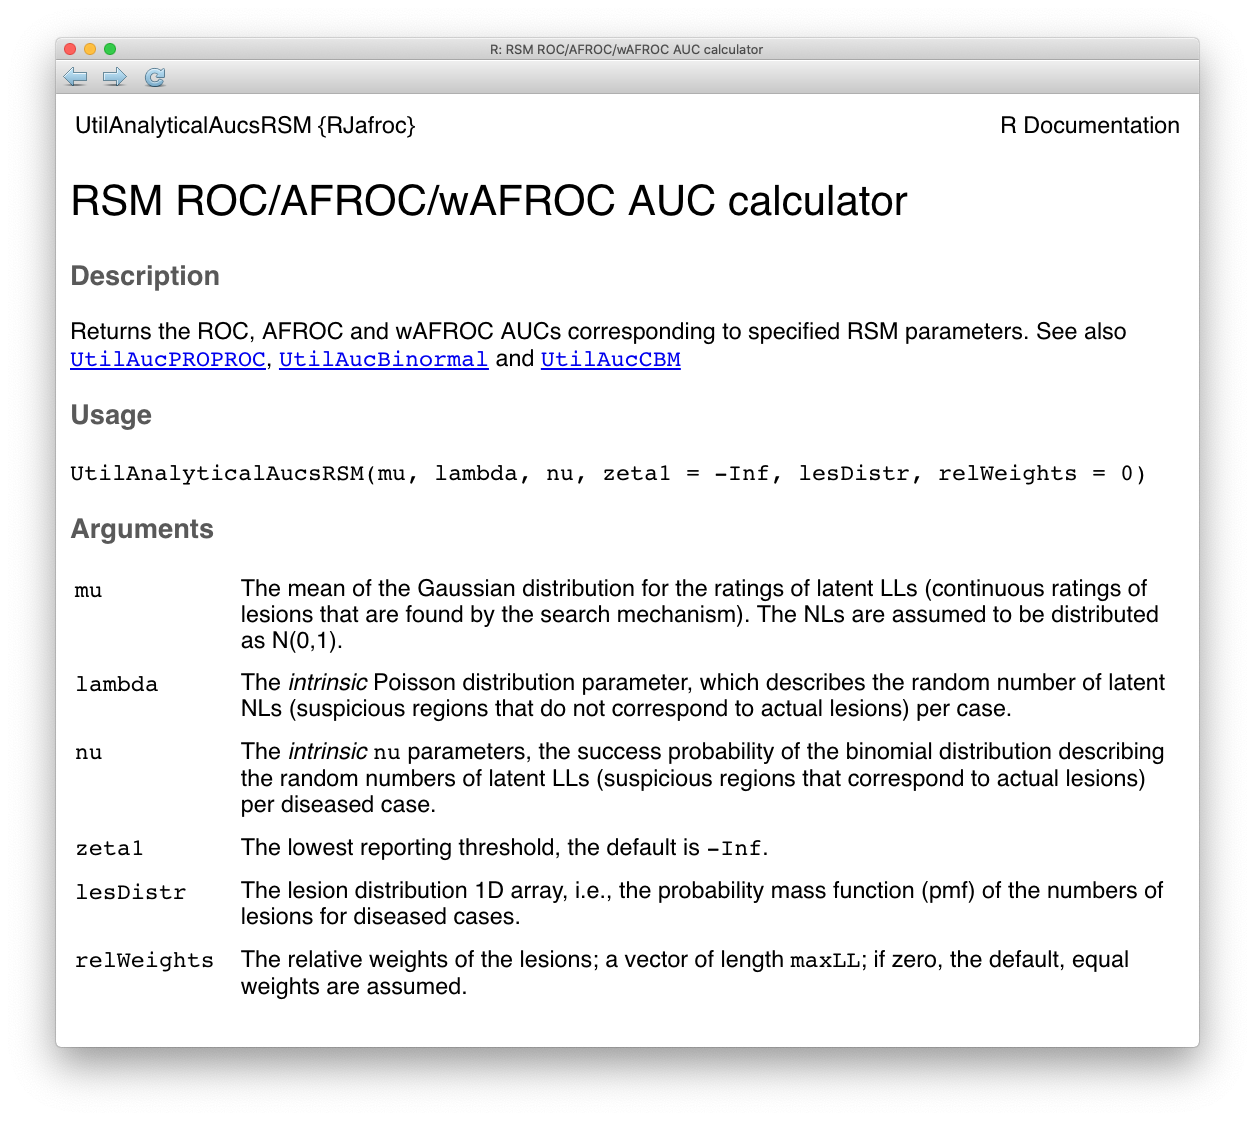
\includegraphics[width=300pt]{images/rsm-predictions/util-analytical-aucs-rsm} 

}

\caption{Help page for `RJafroc` function `UtilAnalyticalAucsRSM`.}\label{fig:rsm-predictions-help}
\end{figure}

The arguments to \texttt{UtilAnalyticalAucsRSM()} are the intrinsic RSM parameters \(\mu\), \(\lambda\), \(\nu\) and \(\zeta\). The default value of \(\zeta\) is \(\zeta = -\infty\). The remaining arguments \texttt{lesDistr} and \texttt{relWeights} are not RSM parameters per se, rather they specify the lesion-richness of the diseased cases and the relative lesion weights (not needed for computing ROC AUC). The dimensions of \texttt{lesDistr} and \texttt{relWeights} are each equal to the maximum number of lesions per case \(L_{max}\). In the following code \(L_{max} = 3\) and \texttt{lesDistr\ \textless{}-\ c(0.5,\ 0.3,\ 0.2)}, meaning 50 percent of diseased cases have one lesion per case, 30 percent have two lesions and 20 percent have three lesions.

The function returns a list containing the AUCs under the ROC and other operating characteristics.

\begin{Shaded}
\begin{Highlighting}[]
\NormalTok{mu }\OtherTok{\textless{}{-}} \DecValTok{1}\NormalTok{; lambda }\OtherTok{\textless{}{-}} \DecValTok{1}\NormalTok{; nu }\OtherTok{\textless{}{-}} \DecValTok{1}
\NormalTok{lesDistr }\OtherTok{\textless{}{-}} \FunctionTok{c}\NormalTok{(}\FloatTok{0.5}\NormalTok{, }\FloatTok{0.3}\NormalTok{, }\FloatTok{0.2}\NormalTok{) }\CommentTok{\# implies L\_max = 3}
\NormalTok{aucs }\OtherTok{\textless{}{-}} \FunctionTok{UtilAnalyticalAucsRSM}\NormalTok{(}\AttributeTok{mu =}\NormalTok{ mu, }
                              \AttributeTok{lambda =}\NormalTok{ lambda, }
                              \AttributeTok{nu =}\NormalTok{ nu, }
                              \AttributeTok{lesDistr =}\NormalTok{ lesDistr)}
\FunctionTok{cat}\NormalTok{(}\StringTok{"mu = "}\NormalTok{, mu, }
\StringTok{", lambda = "}\NormalTok{, lambda, }
\StringTok{", nu = "}\NormalTok{, nu,  }
\StringTok{", AUC ROC = "}\NormalTok{, aucs}\SpecialCharTok{$}\NormalTok{aucROC, }\StringTok{"}\SpecialCharTok{\textbackslash{}n}\StringTok{"}\NormalTok{)}
\end{Highlighting}
\end{Shaded}

\begin{verbatim}
## mu =  1 , lambda =  1 , nu =  1 , AUC ROC =  0.8817798
\end{verbatim}

Experimenting with different parameter combinations reveals the following behavior for ROC AUC.

\begin{itemize}
\item
  AUC is an increasing functions of \(\mu\). Increasing perceptual signal-to-noise-ratio leads to improved performance: for background on this important dependence see \ref{froc-paradigm-solar-analogy}. Increasing \(\mu\) increases the separation between the two pdfs defining the ROC curve, which increases AUC. Furthermore, the number of NLs decreases because \(\lambda = \lambda / \mu\) decreases, which increases performance. Finally, \(\nu\) increases approaching unity, which leads to more LLs and increased performance. \emph{Because all three effects reinforce each other, a change in \(\mu\) results in a large effect on performance.}
\item
  AUC increases as \(\lambda\) decreases. Decreasing \(\lambda\) results in fewer NLs which results in increased performance. This is a relatively weak effect.
\item
  AUC increases as \(\nu\) increases. Increasing \(\nu\) results in more LLs being marked, which increases performance. This is a relatively strong effect.
\item
  AUC decreases as \(\zeta\) increases. This important effect is discussed in the next section.
\item
  ROC AUC increases with \(L_{max}\). With more lesions per case, there is increased probability that that at least one of them will result in a LL, and the diseased case pdf moves to the right, both of which result in increased performance.
\item
  ROC AUC increases as \texttt{lesDistr} is weighted towards more lesions per case. For example, \texttt{lesDistr\ \textless{}-\ c(0,\ 0,\ 1)} (all cases have 3 lesions per case) will yield higher performance than \texttt{lesDistr\ \textless{}-\ c(1,\ 0,\ 0)} (all cases have one lesion per case).
\end{itemize}

\hypertarget{comparing-tpf-formula-to-rjafroc-functions}{%
\subsection{\texorpdfstring{Comparing TPF formula to \texttt{RJafroc} functions}{Comparing TPF formula to RJafroc functions}}\label{comparing-tpf-formula-to-rjafroc-functions}}

A hand calculation is shown and compared to the value yielded by the function \texttt{RSM\_TPF}. The RSM parameters and the value of \(\zeta\) are:

\begin{Shaded}
\begin{Highlighting}[]
\NormalTok{zeta }\OtherTok{\textless{}{-}} \DecValTok{1}
\NormalTok{mu }\OtherTok{\textless{}{-}} \DecValTok{2}
\NormalTok{lambda }\OtherTok{\textless{}{-}} \DecValTok{1}
\NormalTok{nu }\OtherTok{\textless{}{-}} \FloatTok{0.9}
\NormalTok{lesDistr }\OtherTok{\textless{}{-}} \FunctionTok{c}\NormalTok{(}\FloatTok{0.5}\NormalTok{,}\FloatTok{0.5}\NormalTok{)}
\end{Highlighting}
\end{Shaded}

The \texttt{lesDistr} vector corresponds to \(f_L\) and specifies \(L_{max} = 2\) and 50 percent of diseased cases have one lesion per case and the rest have two lesions per case.

Direct implementation of Eqn. \eqref{eq:rsm-predictions-tpf2} followed by usage of the function \texttt{RSM\_TPF} follows:

\begin{Shaded}
\begin{Highlighting}[]
\FunctionTok{cat}\NormalTok{(}\DecValTok{1}\SpecialCharTok{{-}}
\FunctionTok{exp}\NormalTok{(}\SpecialCharTok{{-}}\NormalTok{lambda}\SpecialCharTok{*}\FunctionTok{pnorm}\NormalTok{(}\SpecialCharTok{{-}}\NormalTok{zeta))}\SpecialCharTok{*}
\NormalTok{(lesDistr[}\DecValTok{1}\NormalTok{]}\SpecialCharTok{*}\NormalTok{(}\DecValTok{1}\SpecialCharTok{{-}}\NormalTok{nu}\SpecialCharTok{*}\FunctionTok{pnorm}\NormalTok{(mu}\SpecialCharTok{{-}}\NormalTok{zeta))}\SpecialCharTok{+}
\NormalTok{lesDistr[}\DecValTok{2}\NormalTok{]}\SpecialCharTok{*}\NormalTok{(}\DecValTok{1}\SpecialCharTok{{-}}\NormalTok{nu}\SpecialCharTok{*}\FunctionTok{pnorm}\NormalTok{(mu}\SpecialCharTok{{-}}\NormalTok{zeta))}\SpecialCharTok{\^{}}\DecValTok{2}\NormalTok{))}
\end{Highlighting}
\end{Shaded}

\begin{verbatim}
## 0.8712655
\end{verbatim}

\begin{Shaded}
\begin{Highlighting}[]
\FunctionTok{cat}\NormalTok{(}\FunctionTok{RSM\_TPF}\NormalTok{(zeta,mu,lambda,nu, }\AttributeTok{lesDistr =}\NormalTok{ lesDistr))}
\end{Highlighting}
\end{Shaded}

\begin{verbatim}
## 0.8712655
\end{verbatim}

The two values are identical.

\hypertarget{effect-on-operating-point-of-varying-rsm-parameters}{%
\subsection{Effect on operating point of varying RSM parameters}\label{effect-on-operating-point-of-varying-rsm-parameters}}

It is instructive to understand the effects of varying the RSM parameters on the operating point on the ROC curve.

\hypertarget{vary-mu}{%
\subsubsection{\texorpdfstring{Vary \(\mu\)}{Vary \textbackslash mu}}\label{vary-mu}}

\begin{verbatim}
## lesDistr =  0.1 0.9
\end{verbatim}

\begin{verbatim}
## Varying mu only: 
## Other parameters are lambda =  2 , nu =  0.5 , zeta =  0
\end{verbatim}

\begin{verbatim}
## mu = 0 , RSM-x = 0.6321 , RSM-y = 0.7862 
## mu = 0.5 , RSM-x = 0.6321 , RSM-y = 0.8342 
## mu = 1 , RSM-x = 0.6321 , RSM-y = 0.8676 
## mu = 1.5 , RSM-x = 0.6321 , RSM-y = 0.8862 
## mu = 2 , RSM-x = 0.6321 , RSM-y = 0.8946 
## mu = 2.5 , RSM-x = 0.6321 , RSM-y = 0.8977 
## mu = 3 , RSM-x = 0.6321 , RSM-y = 0.8986 
## mu = 3.5 , RSM-x = 0.6321 , RSM-y = 0.8988 
## mu = 4 , RSM-x = 0.6321 , RSM-y = 0.8988 
## mu = 4.5 , RSM-x = 0.6321 , RSM-y = 0.8988 
## mu = 5 , RSM-x = 0.6321 , RSM-y = 0.8988
\end{verbatim}

The abscissa is independent of \(\mu\) (because this parameter has no effect on non-diseased cases) and the ordinate is an increasing function of \(\mu\) (as expected for increasing separation of the LL and NL distributions; the LLs on diseased cases are rated higher causing the distribution of \(h_2\) to shift to higher values).

\hypertarget{vary-lambda}{%
\subsubsection{\texorpdfstring{Vary \(\lambda\)}{Vary \textbackslash lambda}}\label{vary-lambda}}

\begin{verbatim}
## lesDistr =  0.1 0.9
\end{verbatim}

\begin{verbatim}
## Varying lambda only: 
## Other parameters are mu =  1 , nu =  0.5 , zeta =  0
\end{verbatim}

\begin{verbatim}
## lambda = 0.5 , RSM-x = 0.2212 , RSM-y = 0.7196 
## lambda = 1 , RSM-x = 0.3935 , RSM-y = 0.7817 
## lambda = 1.5 , RSM-x = 0.5276 , RSM-y = 0.8300 
## lambda = 2 , RSM-x = 0.6321 , RSM-y = 0.8676 
## lambda = 2.5 , RSM-x = 0.7135 , RSM-y = 0.8969 
## lambda = 3 , RSM-x = 0.7769 , RSM-y = 0.9197 
## lambda = 3.5 , RSM-x = 0.8262 , RSM-y = 0.9374 
## lambda = 4 , RSM-x = 0.8647 , RSM-y = 0.9513 
## lambda = 4.5 , RSM-x = 0.8946 , RSM-y = 0.9621 
## lambda = 5 , RSM-x = 0.9179 , RSM-y = 0.9705
\end{verbatim}

The abscissa increases with \(\lambda\) (more NLs on non-diseased cases are generated causing the distribution of \(h_1\) to shift to higher values) and the ordinate also increases with \(\lambda\) (more NLs on diseased cases are generated causing the distribution of \(h_2\) to shift to higher values - recall that on diseased cases the highest z-sample is the maximum of NL and LL z-samples, whichever is highest).

\hypertarget{vary-nu}{%
\subsubsection{\texorpdfstring{Vary \(\nu\)}{Vary \textbackslash nu}}\label{vary-nu}}

\begin{verbatim}
## lesDistr =  0.1 0.9
\end{verbatim}

\begin{verbatim}
## Varying nu only: 
## Other parameters are mu =  1 , lambda =  2 , zeta =  0
\end{verbatim}

\begin{verbatim}
## nu = 0 , RSM-x = 0.6321 , RSM-y = 0.6321 
## nu = 0.1 , RSM-x = 0.6321 , RSM-y = 0.6886 
## nu = 0.2 , RSM-x = 0.6321 , RSM-y = 0.7404 
## nu = 0.3 , RSM-x = 0.6321 , RSM-y = 0.7875 
## nu = 0.4 , RSM-x = 0.6321 , RSM-y = 0.8299 
## nu = 0.5 , RSM-x = 0.6321 , RSM-y = 0.8676 
## nu = 0.6 , RSM-x = 0.6321 , RSM-y = 0.9006 
## nu = 0.7 , RSM-x = 0.6321 , RSM-y = 0.9289 
## nu = 0.8 , RSM-x = 0.6321 , RSM-y = 0.9526 
## nu = 0.9 , RSM-x = 0.6321 , RSM-y = 0.9716
\end{verbatim}

No effect on the abscissa as \(\nu\) increases (this parameter has no effect on non-diseased case sampling) and the ordinate increases with \(\nu\) (more LLs on diseased cases, as more lesions are localized, causing the distribution of \(h_2\) to shift to higher values).

\hypertarget{vary-zeta}{%
\subsubsection{\texorpdfstring{Vary \(\zeta\)}{Vary \textbackslash zeta}}\label{vary-zeta}}

\begin{verbatim}
## lesDistr =  0.1 0.9
\end{verbatim}

\begin{verbatim}
## Varying zeta only: 
## Other parameters are mu =  1 , lambda =  2 , nu =  0.5
\end{verbatim}

\begin{verbatim}
## zeta = -3 , RSM-x = 0.8643 , RSM-y = 0.9627 
## zeta = -2.5 , RSM-x = 0.8630 , RSM-y = 0.9623 
## zeta = -2 , RSM-x = 0.8584 , RSM-y = 0.9610 
## zeta = -1.5 , RSM-x = 0.8453 , RSM-y = 0.9570 
## zeta = -1 , RSM-x = 0.8141 , RSM-y = 0.9467 
## zeta = -0.5 , RSM-x = 0.7492 , RSM-y = 0.9224 
## zeta = 0 , RSM-x = 0.6321 , RSM-y = 0.8676 
## zeta = 0.5 , RSM-x = 0.4605 , RSM-y = 0.7568 
## zeta = 1 , RSM-x = 0.2719 , RSM-y = 0.5768 
## zeta = 1.5 , RSM-x = 0.1251 , RSM-y = 0.3628 
## zeta = 2 , RSM-x = 0.0445 , RSM-y = 0.1831 
## zeta = 2.5 , RSM-x = 0.0123 , RSM-y = 0.0740 
## zeta = 3 , RSM-x = 0.0027 , RSM-y = 0.0241
\end{verbatim}

Increasing \(\zeta\) causes the operating point to move down the ROC.

\hypertarget{vary-f_l}{%
\subsubsection{\texorpdfstring{Vary \(f_L\)}{Vary f\_L}}\label{vary-f_l}}

The \texttt{lesDist} vector is defined as \((f, (1-f))\) where f is varied from 1 (only cases with one lesion per case) to 0 (only cases with two lesions per case):

\begin{verbatim}
## lesDistr =  (f, 1-f)
\end{verbatim}

\begin{verbatim}
## Varying f only: 
## Other parameters are mu =  1 , lambda =  2 , nu =  0.5 , zeta =  0
\end{verbatim}

\begin{verbatim}
## f =  1 , RSM-x =  0.6321 , RSM-y =  0.7869 
## f =  0.9 , RSM-x =  0.6321 , RSM-y =  0.7958 
## f =  0.8 , RSM-x =  0.6321 , RSM-y =  0.8048 
## f =  0.7 , RSM-x =  0.6321 , RSM-y =  0.8138 
## f =  0.6 , RSM-x =  0.6321 , RSM-y =  0.8227 
## f =  0.5 , RSM-x =  0.6321 , RSM-y =  0.8317 
## f =  0.4 , RSM-x =  0.6321 , RSM-y =  0.8407 
## f =  0.3 , RSM-x =  0.6321 , RSM-y =  0.8496 
## f =  0.2 , RSM-x =  0.6321 , RSM-y =  0.8586 
## f =  0.1 , RSM-x =  0.6321 , RSM-y =  0.8676 
## f =  0 , RSM-x =  0.6321 , RSM-y =  0.8765
\end{verbatim}

No effect on FPF but TPF increases as more lesions per case means more LLs per case and the distribution of \(h_2\) moves to higher values.

\hypertarget{rsm-predictions-roc-curves}{%
\subsection{Sample ROC curves}\label{rsm-predictions-roc-curves}}

\begin{figure}
\centering
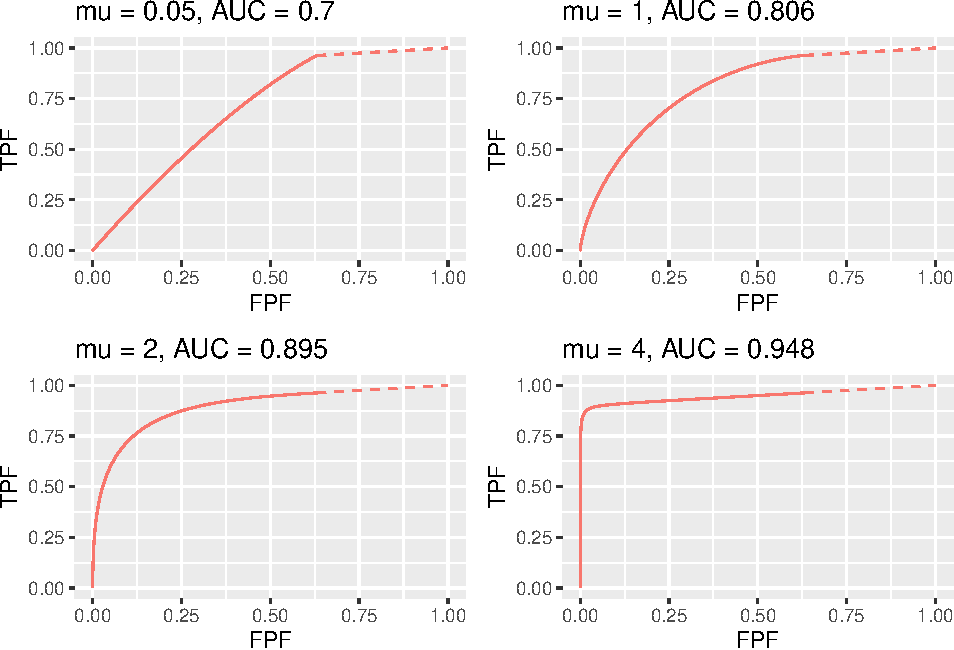
\includegraphics{07-rsm-predictions1_files/figure-latex/rsm-predictions-fig-auc-mu-plots-1.pdf}
\caption{\label{fig:rsm-predictions-fig-auc-mu-plots}ROC curves for indicated values of the \(\mu\) parameter. Notice the transition, as \(\mu\) increases, from near chance level performance to almost perfect performancea as the end-point moves from near (1,1) to near (0,1).}
\end{figure}

Fig. \ref{fig:rsm-predictions-fig-auc-mu-plots} displays ROC curves for indicated values of \(\mu\). The remaining RSM model parameters are \(\lambda = 1\), \(\nu = 1\) and \(\zeta = -\infty\) and there is one lesion per diseased case.

The following are evident from these figures:

\begin{enumerate}
\def\labelenumi{\arabic{enumi}.}
\tightlist
\item
  As \(\mu\) increases the ROC curve more closely approaches the upper-left corner of the ROC plot. This signifies increasing performance and the area under the ROC and AFROC curves approach unity. The end-point abscissa decreases, meaning increasing numbers of unmarked non-diseased cases, i.e., more perfect decisions on non-diseased cases. The end-point ordinate increases, meaning decreasing numbers of unmarked lesions, i.e., more good decisions on diseased cases.
\item
  For \(\mu\) close to zero the operating characteristic approaches the chance diagonal and the area under the ROC curve approaches 0.5.
\item
  The area under the ROC increases monotonically from 0.5 to 1 as \(\mu\) increases from zero to infinity.
\item
  For large \(\mu\) the accessible portion of the operating characteristic approaches the vertical line connecting (0,0) to (0,1), the area under which is zero. The complete ROC curve is obtained by connecting this point to (1,1) by the dashed line and in this limit the area under the complete ROC curve approaches unity. Omitting the area under the dashed portion of the curve will result in a severe underestimate of true performance.
\item
  As \(L_{max}\) increases (allowed values are 1, 2, 3, etc.) the area under the ROC curve increases, approaching unity and \(\text{TPF}_{\text{max}}\) approaches unity. With more lesions per diseased case, the chances are higher that at least one of them will be found and marked. However, \(\text{FPF}_{\text{max}}\) remains constant as determined by the constant value of \(\lambda = \frac{\lambda}{\mu}\), Eqn. \eqref{eq:rsm-predictions-fpf-max}
\item
  As \(\lambda\) decreases \(\text{FPF}_{\text{max}}\) decreases to zero and \(\text{TPF}_{\text{max}}\) decreases. The decrease in \(\text{TPF}_{\text{max}}\) is consistent with the fact that, with fewer NLs, there is less chance of a NL being rated higher than a LL, and one is completely dependent on at least one lesion being found.
\item
  As \(\nu\) increases \(\text{FPF}_{\text{max}}\) stays constant at the value determined by \(\lambda\) and \(\mu\), while \(\text{TPF}_{\text{max}}\) approaches unity. The corresponding physical parameter \(\nu\) increases approaching unity, guaranteeing every lesion will be found.
\end{enumerate}

\hypertarget{rsm-predictions-pdf-curves}{%
\subsection{Sample RSM pdf curves}\label{rsm-predictions-pdf-curves}}

\begin{figure}
\centering
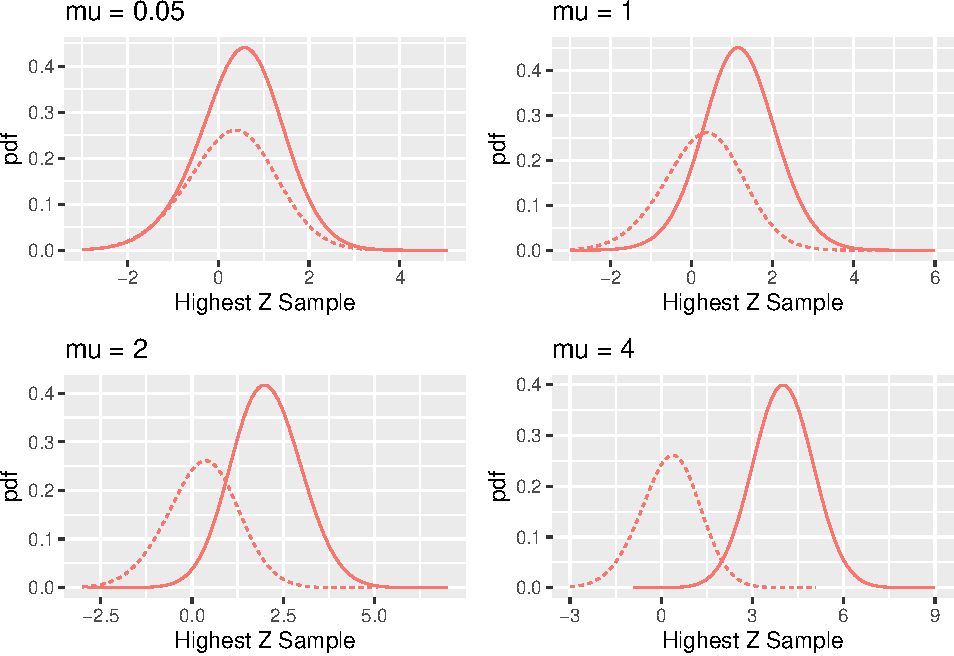
\includegraphics{07-rsm-predictions1_files/figure-latex/rsm-predictions-fig-pdf-mu-plots-1.pdf}
\caption{\label{fig:rsm-predictions-fig-pdf-mu-plots}RSM pdf curves for indicated values of the \(\mu\) parameter. The solid curve corresponds to diseased cases and the dotted curve corresponds to non-diseased cases.}
\end{figure}

Fig. \ref{fig:rsm-predictions-fig-pdf-mu-plots} shows pdf plots for the same values of parameters as in Fig. \ref{fig:rsm-predictions-fig-auc-mu-plots}.

Consider the plot of the pdfs for \(\mu = 1\). Since the integral of a pdf function over an interval amounts to counting the fraction of events occurring in the interval, it should be evident that the area under the non-diseased pdf equals \(\text{FPF}_{\text{max}}\) and that under the diseased pdf equals \(\text{TPF}_{\text{max}}\). For the chosen value \(\lambda = 1\) one has \(\text{FPF}_{\text{max}} = 1 - e^{-\lambda} = 0.632\). The area under the non-diseased pdf is less than unity because it is missing the contribution of non-diseased cases with no marks, the probability of which is \(e^{-\lambda} = e^{-1} = 0.368\). Equivalently, it is missing the area under the dashed straight line segment of the ROC curve. Likewise, the area under the diseased pdf equals \(\text{TPF}_{\text{max}}\), Eqn. \eqref{eq:rsm-predictions-tpf-max}, which is also less than unity. For the chosen values of \(\mu = \lambda = \nu = L = 1\) it equals \(\text{TPF}_{\text{max}} = 1 - e^{-\lambda} e^{-\nu} = 0.865\). This area is somewhat larger than that under the non-diseased pdf, as is evident from visual examination of the plot. A greater fraction of diseased cases generate marks than do non-diseased cases, consistent with the presence of lesions in diseased cases. The complement of 0.865 is due to diseased cases with no marks, which account for a fraction 0.135 of diseased cases. To summarize, the pdf's do not integrate to unity for the reason that the integrals account only for the continuous section of the ROC curve and do not include cases with zero latent marks that do not generate z-samples. The effect becomes more exaggerated for higher values of \(\mu\) as this causes \(\text{FPF}_{\text{max}}\) to further decrease.

The plot in Fig. \ref{fig:rsm-predictions-fig-pdf-mu-plots} labeled \(\mu = 0.05\) may be surprising. Since it corresponds to a small value of \(\mu\), one may expect both pdfs to overlap and be centered at zero. Instead, while they do overlap, the shape is distinctly non-Gaussian and centered at approximately 1.8. This is because the small value of \(\mu\) results in a large value of the \(\lambda\) parameter, since \(\lambda = \lambda / \mu = 20\). The highest of a large number of samples from the unit normal distribution is not normal and is peaked at a value above zero \citep{fisher1928limiting}.

\hypertarget{rsm-predictions-roc-curve-proper}{%
\section{Proper ROC curve}\label{rsm-predictions-roc-curve-proper}}

\begin{quote}
A proper ROC curve has the property that it never crosses the chance diagonal and its slope never increases as the operating point moves up the ROC curve \citep{metz1999proper, macmillan2004detection}. \emph{It is shown below that the RSM predicted ROC curve, including the dashed straight line extension, is proper} \footnote{The statement in the print book that the ``proper'' property only applies to the continuous section is incorrect.}.
\end{quote}

Consider first the continuous section which is below-left of the end-point. For convenience one abbreviates FPF and TPF to \(x\) and \(y\), respectively, and suppresses the dependence on model parameters. From Eqn. \eqref{eq:rsm-predictions-fpf} and Eqn. \eqref{eq:rsm-predictions-tpf2} one can express the ROC coordinates as:

\begin{equation}
\left. 
\begin{aligned}
x\left ( \zeta \right ) =& 1 - G\left ( \zeta \right )\\
y\left ( \zeta \right ) =& 1 - F\left ( \zeta \right ) G\left ( \zeta \right ) 
\end{aligned}
\right \}
\label{eq:rsm-predictions-f-g}
\end{equation}

where:

\begin{equation}
\left. 
\begin{aligned}
G\left ( \zeta \right ) =& \text{exp}\left ( -\lambda \Phi \left ( -\zeta \right )\right )\\
F\left ( \zeta \right ) =& \sum_{L=1}^{L_{max}} f_L  \left ( 1 - \nu \Phi \left ( \mu -\zeta \right ) \right )^L 
\end{aligned}
\right \}
\label{eq:rsm-predictions-fg-defs}
\end{equation}

\begin{quote}
These equations have the same structure as \citep{swensson1996unified} Eqns. 1 and 2 and the logic used there to demonstrate that ROC curves predicted by Swensson's LROC model is proper also applies to the present situation.
\end{quote}

Specifically, since the \(\Phi\) function ranges between 0 and 1 and \(0 \leq \nu \leq 1\), it follows that \(F\left ( \zeta \right ) \leq 1\). Therefore \(y\left ( \zeta \right ) \geq x\left ( \zeta \right )\) and the ROC curve is constrained to the upper half of the ROC space, namely the portion above the chance diagonal. Additionally, the more general constraint shown by Swensson applies, namely the slope of the ROC curve at any operating point (x, y) cannot be less than the slope of the dashed straight line connecting (x, y) and \(\left (\text{FPF}_{\text{max}}, \text{TPF}_{\text{max}} \right )\), the coordinates of the RSM end-point. This implies that the slope decreases monotonically and also rules out curves with ``hooks''.

\begin{quote}
In Appendix 1 \ref{rsm-predictions-appendix1} it is shown analytically that the slope is continuous at the end-point transition from the continuous curve to the dashed straight line. In Appendix 2 \ref{rsm-predictions-appendix2} the slope near the end-point is examined numerically to resolve an apparent paradox, namely the ROC plot can appear discontinuous at the end-point when in fact no discontinuity exists.
\end{quote}

\hypertarget{rsm-predictions-roc-curve-aucs-zeta1}{%
\section{\texorpdfstring{\(\zeta\) dependence of ROC AUC}{\textbackslash zeta dependence of ROC AUC}}\label{rsm-predictions-roc-curve-aucs-zeta1}}

When it comes to predicted ROC AUC there is an important difference between conventional ROC models and the RSM. The former has no dependence on \(\zeta\). This is because in the ROC model every case yields a rating, no matter how low the z-sample, implying that effectively \(\zeta = -\infty\). The lack of \(\zeta\) dependence is demonstrated by the help page for function \texttt{UtilAucBormal}, shown below, which depends on only two parameters, \(a\) and \(b\) (the two-parameter dependence is also true for other ROC models implemented in \texttt{RJafroc}, e.g., \texttt{UtilAucCBM} and \texttt{UtilAucPROPROC}).

\begin{figure}

{\centering 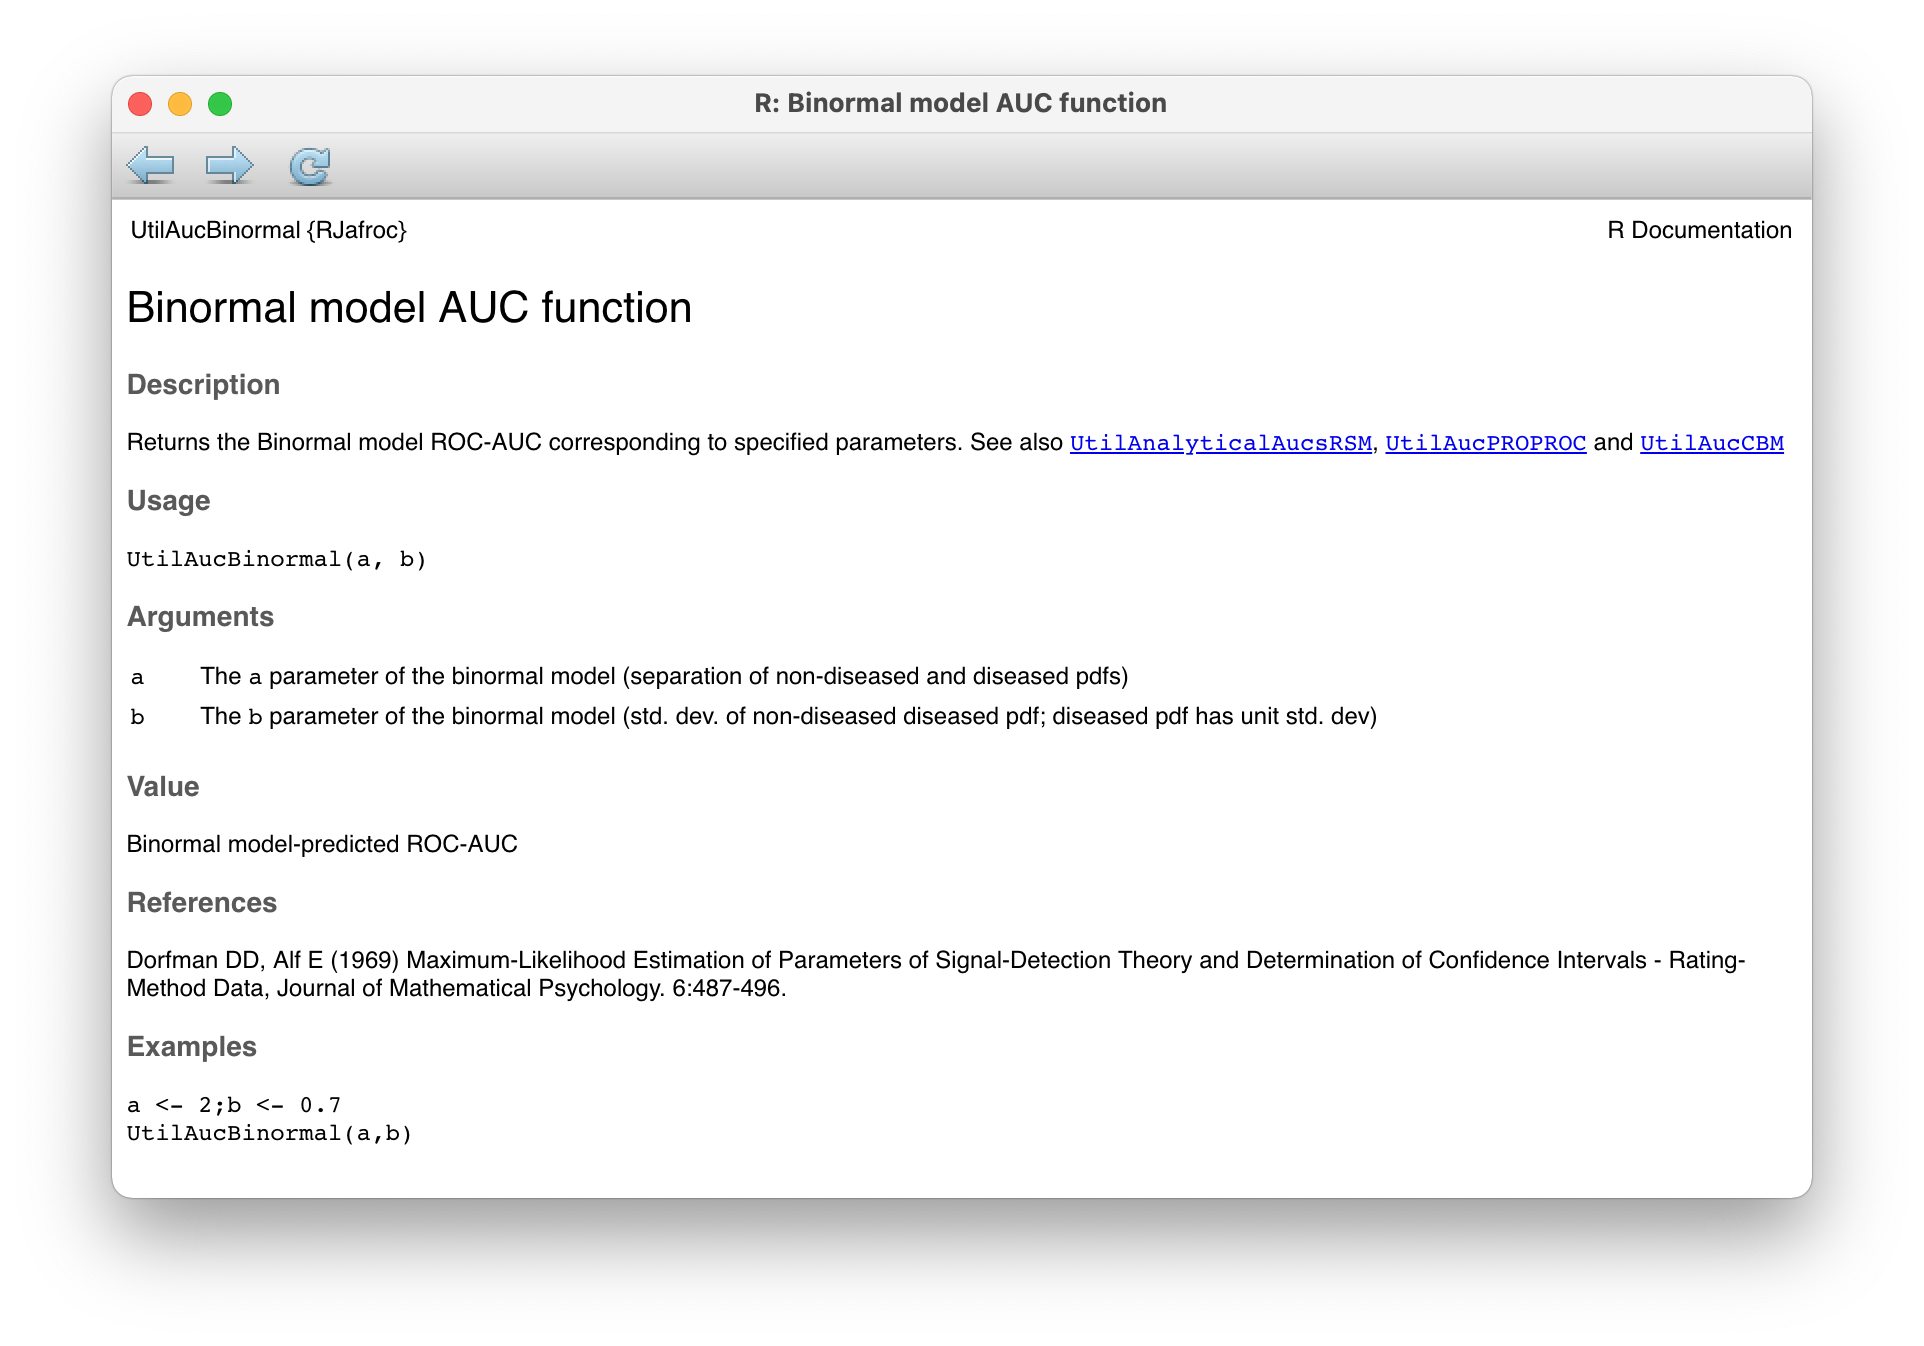
\includegraphics[width=300pt]{images/rsm-predictions/util-aucs-binormal} 

}

\caption{Help page for `RJafroc` function `UtilAucBormal`.}\label{fig:rsm-predictions-binorml-help}
\end{figure}

In contrast, in addition to the basic RSM parameters, i.e., \(\mu\), \(\lambda\) and \(\nu\), the rsm-predictions have an additional dependence on \(\zeta\). This is because the value of \(\zeta\) determines the location of the end-point. The \(\zeta\) dependence is demonstrated next for the ROC plots, but it is true for all RSM predictions.

\begin{figure}

{\centering 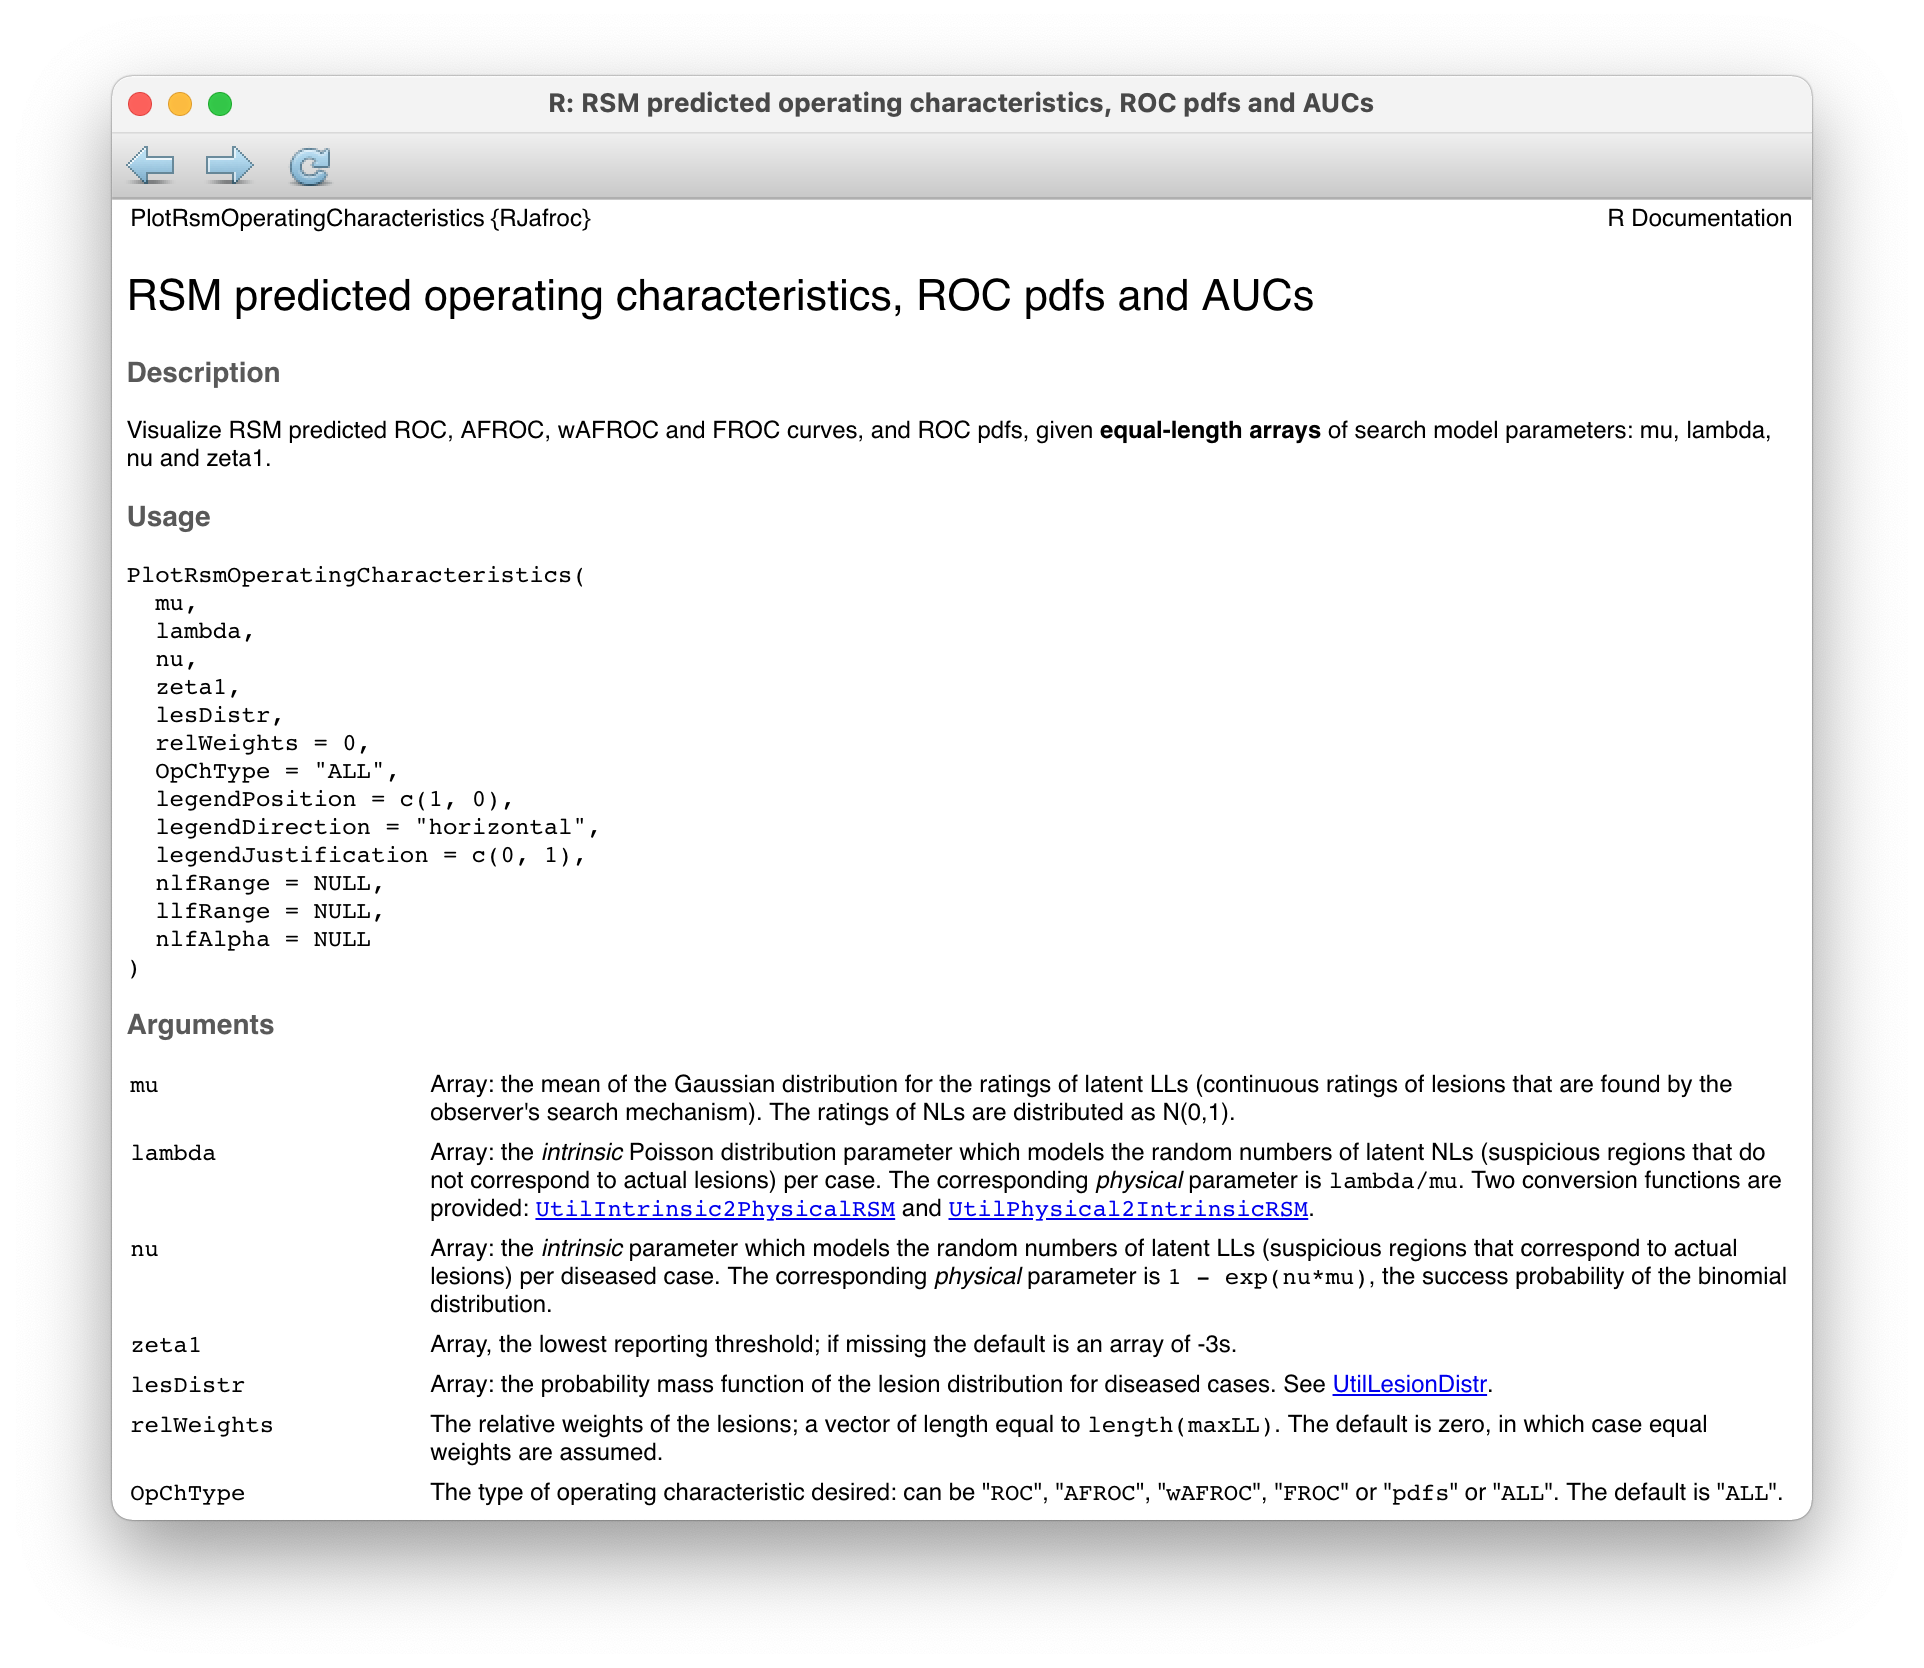
\includegraphics[width=300pt]{images/rsm-predictions/PlotRsmOperatingCharacteristics} 

}

\caption{Help page for `RJafroc` function `PlotRsmOperatingCharacteristics`.}\label{fig:rsm-predictions-operating-characteristics-help}
\end{figure}

The dependence is demonstrated next for two values: \(zeta = -10\) and \(zeta = 1\). The common parameter values are \(\mu = 2\), \(\lambda = 1\), \(\nu = 1\), as shown in the following code-chunk.

\begin{Shaded}
\begin{Highlighting}[]
\NormalTok{roc }\OtherTok{\textless{}{-}} \FunctionTok{PlotRsmOperatingCharacteristics}\NormalTok{(}
     \AttributeTok{mu =} \FunctionTok{c}\NormalTok{(}\DecValTok{2}\NormalTok{,}\DecValTok{2}\NormalTok{),}
     \AttributeTok{lambda =} \FunctionTok{c}\NormalTok{(}\DecValTok{1}\NormalTok{,}\DecValTok{1}\NormalTok{),}
     \AttributeTok{nu =} \FunctionTok{c}\NormalTok{(}\DecValTok{1}\NormalTok{,}\DecValTok{1}\NormalTok{),}
     \AttributeTok{zeta1 =} \FunctionTok{c}\NormalTok{(}\SpecialCharTok{{-}}\DecValTok{10}\NormalTok{, }\DecValTok{1}\NormalTok{),}
     \AttributeTok{lesDistr =} \FunctionTok{c}\NormalTok{(}\FloatTok{0.5}\NormalTok{, }\FloatTok{0.5}\NormalTok{),}
     \AttributeTok{relWeights =} \FunctionTok{c}\NormalTok{(}\FloatTok{0.5}\NormalTok{, }\FloatTok{0.5}\NormalTok{),}
     \AttributeTok{OpChType =} \StringTok{"ROC"}\NormalTok{,}
     \AttributeTok{legendPosition =} \StringTok{"null"}
\NormalTok{)}
\end{Highlighting}
\end{Shaded}

Clearly the red curve has higher AUC. The specific values are 0.9591597 for the red curve and 0.9337196 for the green curve.

\begin{figure}
\centering
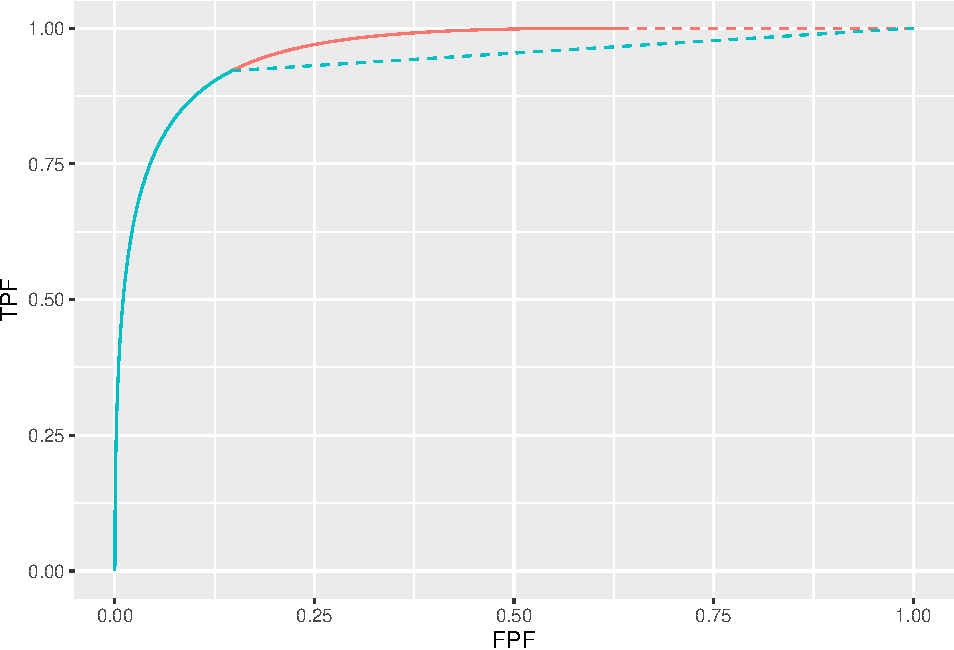
\includegraphics{07-rsm-predictions1_files/figure-latex/rsm-predictions-roc-zeta1-1.pdf}
\caption{\label{fig:rsm-predictions-roc-zeta1}ROC curves for two values of \(\zeta\): both curves correspond to \(\mu = 2\), \(\nu = 1\) and \(\lambda = 1\). The red curve corresponds to \(\zeta = -10\) and the blue curve to \(\zeta = 1\).}
\end{figure}

A consequence of the \(\zeta\) dependence is that if one uses ROC AUC as the measure of performance, the optimal threshold is \(\zeta = -\infty\). In particular, a CAD algorithm that generates FROC data should show all generated marks to the radiologist, which is clearly incorrect and is not adopted by any CAD designer. Selecting the optimal value of the reporting threshold is addressed in Chapter \ref{optim-op-point}.

\hypertarget{rsm-predictions-discussion-summary}{%
\section{TBA Discussion / Summary}\label{rsm-predictions-discussion-summary}}

ROC, FROC and AFROC curves were derived (wAFROC is implemented in the RJafroc). These were used to demonstrate that the FROC is a poor descriptor of performance. Since almost all work to date, including some by me TBA 47,48, has used FROC curves to measure performance, this is going to be difficulty for some to accept. The examples in Fig. 17.6 (A- F) and Fig. 17.7 (A-B) should convince one that the FROC curve is indeed a poor measure of performance. The only situation where one can safely use the FROC curve is if the two modalities produce curves extending over the same NLF range. This can happen with two variants of a CAD algorithm, but rarely with radiologist observers.

A unique feature is that the RSM provides measures of search and lesion-classification performance. It bears repeating that search performance is the ability to find lesions while avoiding finding non-lesions. Search performance can be determined from the position of the ROC end-point (which in turn is determined by RSM-based fitting of ROC data, Chapter 19). The perpendicular distance between the end-point and the chance diagonal is, apart from a factor of 1.414, a measure of search performance. All ROC models that predict continuous curves extending to (1,1), imply zero search performance.

Lesion-classification performance is measured by the AUC value corresponding to the parameter. Lesion-classification performance is the ability to discriminate between LLs and NLs, not between diseased and non-diseased cases: the latter is measured by RSM-AUC. There is a close analogy between the two ways of measuring lesion-classification performance and CAD used to find lesions in screening mammography vs.~CAD used in the diagnostic context to determine if a lesion found at screening is actually malignant. The former is termed CADe, for CAD detection, which in my opinion, is slightly misleading as at screening lesions are found not detected (``detection'' is ``discover or identify the presence or existence of something'', correct localization is not necessarily implied; the more precise term is ``localize''). In the diagnostic context one has CADx, for CAD diagnostic, i.e., given a specific region of the image, is the region malignant?

Search and lesion-classification performance can be used as ``diagnostic aids'' to optimize performance of a reader. For example, is search performance is low, then training using mainly non-diseased cases is called for, so the resident learns the different variants of non-diseased tissues that can appear to be true lesions. If lesion-classification performance is low then training with diseased cases only is called for, so the resident learns the distinguishing features characterizing true lesions from non-diseased tissues that fake true lesions.

Finally, evidence for the RSM is summarized. Its correspondence to the empirical Kundel-Nodine model of visual search that is grounded in eye-tracking measurements. It reduces in the limit of large , which guarantees that every case will yield a decision variable sample, to the binormal model; the predicted pdfs in this limit are not strictly normal, but deviations from normality would require very large sample size to demonstrate. Examples were given where even with 1200 cases the binormal model provides statistically good fits, as judged by the chi-square goodness of fit statistic, Table 17.2. Since the binormal model has proven quite successful in describing a large body of data, it satisfying that the RSM can mimic it in the limit of large . The RSM explains most empirical results regarding binormal model fits: the common finding that b \textless{} 1; that b decreases with increasing lesion pSNR (large and / or ); and the finding that the difference in means divided by the difference in standard deviations is fairly constant for a fixed experimental situation, Table 17.3. The RSM explains data degeneracy, especially for radiologists with high expertise.

The contaminated binormal model2-4 (CBM), Chapter 20, which models the diseased distribution as having two peaks, one at zero and the other at a constrained value, also explains the empirical observation that b-parameter \textless{} 1 and data degeneracy. Because it allows the ROC curve to go continuously to (1,1), CBM does not completely account for search performance -- it accounts for search when it comes to finding lesions, but not for avoiding finding non-lesions.

I do not want to leave the impression that RSM is the ultimate model. The current model does not predict satisfaction of search (SOS) effects27-29. Attempts to incorporate SOS effects in the RSM are in the early research stage. As stated earlier, the RSM is a first-order model: a lot of interesting science remains to be uncovered.

\hypertarget{rsm-predictions-appendix1}{%
\section{Appendix 1: Proof of continuity of slope at the end-point}\label{rsm-predictions-appendix1}}

The following proof is adapted from a document supplied by Dr.~Xuetong Zhai, then ( ca. 2017) a graduate student working under the supervision of the author.

The end point coordinates of the continuous part of ROC curve was derived above, Eqn. \eqref{eq:rsm-predictions-fpf-max} for \(\text{FPF}_{\text{max}}\) and Eqn. \eqref{eq:rsm-predictions-tpf-max-vary-l} for \(\text{TPF}_{\text{max}}\). Therefore, the slope \(m_{st}\) of the dashed straight line is:

\begin{equation}
\left. 
\begin{aligned}
m_{st} =& \frac{1-\text{TPF}_{\text{max}}}{1-\text{FPF}_{\text{max}}}\\
=&\frac{\sum_{L=1}^{L_{max}} f_L \left ( 1 - \nu \right )^L
 \text{exp} \left ( - \lambda \right )} {\text{exp} \left ( - \lambda \right )} \\
=& \sum_{L=1}^{L_{max}} f_L \left ( 1 - \nu \right )^L  \\
\end{aligned}
\right \}
\label{eq:rsm-slope-st-line}
\end{equation}

On the continuous section, \(g\equiv\text{FPF}\) and \(h\equiv\text{TPF}\) are defined by \eqref{eq:rsm-predictions-fpf} and \eqref{eq:rsm-predictions-tpf2}, respectively. Therefore,

\begin{equation}
\left. 
\begin{aligned}
g =& 1-\text{exp} \left ( -\lambda \Phi\left ( -\zeta \right ) \right ) \\
h =& 1-\text{exp} \left ( -\lambda \Phi\left ( -\zeta \right ) \right ) \sum_{L=1}^{L_{max}}f_L \left ( 1-\nu\Phi\left ( \mu - \zeta \right ) \right )^{L}
\end{aligned}
\right \}
\label{eq:rsm-predictions-slope-eq3}
\end{equation}

Taking the differentials of these functions with respect to \(\zeta\) it follows that the slope of the ROC is given by:

\begin{equation}
\left. 
\begin{aligned}
\frac{dh}{dg} =& \sum_{L=1}^{L_{max}}  f_L \left ( 1-\nu\Phi\left ( \mu-\zeta \right ) \right )^{L-1}  \times \\
& \left [ \frac{L\nu\phi\left ( \mu-\zeta \right )}{\lambda\phi\left ( -\zeta \right )} + \left ( 1-\nu\Phi \left ( \mu-\zeta \right )\right ) \right ]\\ 
\end{aligned}
\right \} 
\label{eq:rsm-predictions-slope-eq4}
\end{equation}

Using the following result:

\begin{equation}
\left. 
\begin{aligned}
& \lim_{\zeta \rightarrow -\infty} \frac{\phi \left ( \mu-\zeta \right )}{\phi\left ( -\zeta \right )} \\ 
=&\lim_{\zeta \rightarrow -\infty} \frac{\text{exp}\left ( \frac{-\left (\mu-\zeta  \right )^2}{2} \right )}{\text{exp}\left ( \frac{-\zeta^2}{2} \right )} \\
=& \lim_{\zeta \rightarrow -\infty} \text{exp}\left (-\frac{1}{2} \left( \mu^2 - 2\mu\zeta \right)  \right ) \\
=& 0
\end{aligned}
\right \} 
\label{eq:rsm-predictions-slope-eq5}
\end{equation}

it follows that:

\begin{equation}
\left. 
\begin{aligned}
& \lim_{\zeta \rightarrow -\infty} \frac{dh}{dg} \\ 
=& \sum_{L=1}^{L_{max}} f_L \left ( 1-\nu \right )^{L-1} \left ( 1-\nu \right )\\
=& \sum_{L=1}^{L_{max}} f_L \left ( 1-\nu \right )^{L} \\
=& m_{st}
\end{aligned}
\right \} 
\label{eq:rsm-predictions-slope-eq6}
\end{equation}

This proves that the limiting slope of the continuous section of the ROC curve equals that of the dashed straight line connecting the end-point to (1,1).

\hypertarget{rsm-predictions-appendix2}{%
\section{Appendix 2: Numerical illustration of continuity}\label{rsm-predictions-appendix2}}

The code in this section examines the slope of the ROC curve as one approaches the end-point \(\zeta = -\infty\). The RSM parameter values are \(\mu = 0.5\), \(\lambda = 0.1\) and \(\nu = 0.8\), and twenty percent of the diseased cases have one lesion and 80 percent have 2 lesions, i.e.~\texttt{lesDistr} -\textgreater{} c(0.2, 0.8).

\begin{Shaded}
\begin{Highlighting}[]
\NormalTok{mu }\OtherTok{\textless{}{-}} \FloatTok{0.5}
\NormalTok{lambda }\OtherTok{\textless{}{-}} \FloatTok{0.2}
\NormalTok{nu }\OtherTok{\textless{}{-}} \FloatTok{0.8}
\NormalTok{lesDistr }\OtherTok{\textless{}{-}} \FunctionTok{c}\NormalTok{(}\FloatTok{0.2}\NormalTok{, }\FloatTok{0.8}\NormalTok{)}
\end{Highlighting}
\end{Shaded}

One calculates the coordinates of the end-point and the slope of the line connecting it to (1,1).

\begin{Shaded}
\begin{Highlighting}[]
\NormalTok{maxFPF }\OtherTok{\textless{}{-}} \FunctionTok{FPF}\NormalTok{ (}\SpecialCharTok{{-}}\ConstantTok{Inf}\NormalTok{, lambda)}
\NormalTok{maxTPF }\OtherTok{\textless{}{-}} \FunctionTok{TPF}\NormalTok{ (}\SpecialCharTok{{-}}\ConstantTok{Inf}\NormalTok{, mu, lambda, nu, lesDistr)}
\NormalTok{mStLine }\OtherTok{\textless{}{-}}\NormalTok{ (}\DecValTok{1} \SpecialCharTok{{-}}\NormalTok{ maxTPF) }\SpecialCharTok{/}\NormalTok{ (}\DecValTok{1} \SpecialCharTok{{-}}\NormalTok{ maxFPF)}
\end{Highlighting}
\end{Shaded}

The end-point coordinates are (0.1812692, 0.9410514) and the slope is 0.072. Next one calculates and displays the ROC curve.

\begin{Shaded}
\begin{Highlighting}[]
\NormalTok{ret }\OtherTok{\textless{}{-}} \FunctionTok{PlotRsmOperatingCharacteristics}\NormalTok{(}
\NormalTok{  mu,}
\NormalTok{  lambda,}
\NormalTok{  nu,}
  \AttributeTok{zeta1 =} \SpecialCharTok{{-}}\ConstantTok{Inf}\NormalTok{, }
  \AttributeTok{OpChType =} \StringTok{"ROC"}\NormalTok{,}
  \AttributeTok{lesDistr =}\NormalTok{ lesDistr,}
  \AttributeTok{legendPosition =} \StringTok{"none"}
\NormalTok{)}
\end{Highlighting}
\end{Shaded}

\begin{figure}
\centering
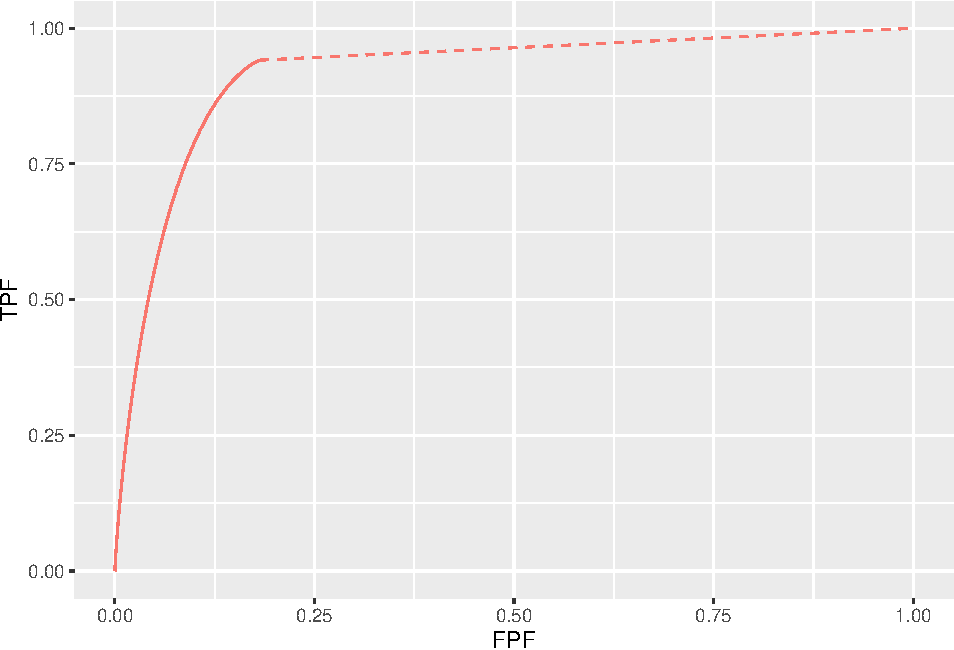
\includegraphics{07-rsm-predictions1_files/figure-latex/rsm-predictions-roc-plot-1.pdf}
\caption{\label{fig:rsm-predictions-roc-plot}ROC curve for selected RSM parameters. The slope of the dashed line is 0.4935272.}
\end{figure}

At first sight the slope appeared to me to be discontinuous at the end-point \footnote{Others have stated a different visual impression.} but this is not true. In fact the slope decreases as one approaches the end-point, and in the limit equals that of the dashed line. This is demonstrated by the next code section which creates a finely-spaced \(\zeta\) array ranging from -3 to -20. These are the points at which the slope is evaluated numerically. Two types of calculations were performed - one using standard \texttt{R} double precision arithmetic and one using multiple precision arithmetic. The R-package \texttt{Rmpfr} was used for the latter. For example, the line \texttt{zeta\_mpr\ -\textgreater{}\ mpfr(zeta,\ 2000)} generates a 2000-bit representation of \(\zeta\). All subsequent computations using \texttt{zeta\_mpr} uses multiple precision arithmetic. The computed slopes are saved in two arrays, \texttt{y1}, the standard precision arithmetic slope and \texttt{y2}, the multiple precision arithmetic slope.

\begin{Shaded}
\begin{Highlighting}[]
\NormalTok{zeta\_arr }\OtherTok{\textless{}{-}} \FunctionTok{c}\NormalTok{(}\FunctionTok{seq}\NormalTok{(}\SpecialCharTok{{-}}\DecValTok{3}\NormalTok{, }\SpecialCharTok{{-}}\DecValTok{5}\NormalTok{, }\SpecialCharTok{{-}}\FloatTok{0.2}\NormalTok{), }\FunctionTok{seq}\NormalTok{(}\SpecialCharTok{{-}}\DecValTok{5}\NormalTok{, }\SpecialCharTok{{-}}\DecValTok{20}\NormalTok{, }\SpecialCharTok{{-}}\FloatTok{0.5}\NormalTok{))}
\NormalTok{y1 }\OtherTok{\textless{}{-}} \FunctionTok{array}\NormalTok{(}\DecValTok{0}\NormalTok{, }\FunctionTok{length}\NormalTok{(zeta\_arr))}
\NormalTok{y2 }\OtherTok{\textless{}{-}} \FunctionTok{array}\NormalTok{(}\DecValTok{0}\NormalTok{, }\FunctionTok{length}\NormalTok{(zeta\_arr))}
\NormalTok{i }\OtherTok{\textless{}{-}} \DecValTok{0}
\ControlFlowTok{for}\NormalTok{ (zeta }\ControlFlowTok{in}\NormalTok{ zeta\_arr) \{}
\NormalTok{  i }\OtherTok{\textless{}{-}}\NormalTok{ i }\SpecialCharTok{+} \DecValTok{1}
  \CommentTok{\# normal precision arithmetic}
\NormalTok{  zeta2 }\OtherTok{\textless{}{-}}\NormalTok{ zeta }\SpecialCharTok{+} \FloatTok{1e{-}6}
\NormalTok{  delta\_FPF }\OtherTok{\textless{}{-}} \FunctionTok{FPF}\NormalTok{ (zeta, lambda) }\SpecialCharTok{{-}} \FunctionTok{FPF}\NormalTok{ (zeta2, lambda)}
\NormalTok{  delta\_TPF }\OtherTok{\textless{}{-}} \FunctionTok{TPF}\NormalTok{ (zeta, mu, lambda, nu, lesDistr) }\SpecialCharTok{{-}} 
    \FunctionTok{TPF}\NormalTok{ (zeta2, mu, lambda, nu, lesDistr)}
\NormalTok{  mAnal }\OtherTok{\textless{}{-}}\NormalTok{ delta\_TPF }\SpecialCharTok{/}\NormalTok{ delta\_FPF}
\NormalTok{  y1[i] }\OtherTok{\textless{}{-}}\NormalTok{ mAnal}
  \CommentTok{\# end normal precision arithmetic}
  
  \CommentTok{\# multiple precision arithmetic}
\NormalTok{  zeta\_mpr }\OtherTok{\textless{}{-}} \FunctionTok{mpfr}\NormalTok{(zeta, }\DecValTok{2000}\NormalTok{) }\CommentTok{\# 2000 digit precision}
\NormalTok{  zeta2\_mpr }\OtherTok{\textless{}{-}}\NormalTok{ zeta\_mpr }\SpecialCharTok{+} \FloatTok{1e{-}12} \CommentTok{\# small increment}
\NormalTok{  delta\_FPF }\OtherTok{\textless{}{-}} \FunctionTok{FPF}\NormalTok{ (zeta\_mpr, lambda) }\SpecialCharTok{{-}} \FunctionTok{FPF}\NormalTok{ (zeta2\_mpr, lambda)}
\NormalTok{  delta\_TPF }\OtherTok{\textless{}{-}} \FunctionTok{TPF}\NormalTok{ (zeta\_mpr, mu, lambda, nu, lesDistr) }\SpecialCharTok{{-}} 
    \FunctionTok{TPF}\NormalTok{ (zeta2\_mpr, mu, lambda, nu, lesDistr)}
\NormalTok{  mAnalRmpfr }\OtherTok{\textless{}{-}}\NormalTok{ delta\_TPF }\SpecialCharTok{/}\NormalTok{ delta\_FPF}
\NormalTok{  temp }\OtherTok{\textless{}{-}} \FunctionTok{as.numeric}\NormalTok{(mAnalRmpfr)}
  \ControlFlowTok{if}\NormalTok{ (}\FunctionTok{is.nan}\NormalTok{(temp))\{}
\NormalTok{    y2[i] }\OtherTok{\textless{}{-}} \ConstantTok{NA}
\NormalTok{  \} }\ControlFlowTok{else}\NormalTok{ y2[i] }\OtherTok{\textless{}{-}}\NormalTok{ temp }
  \CommentTok{\# end multiple precision arithmetic}
\NormalTok{\}}
\end{Highlighting}
\end{Shaded}

The next code section displays 3 plots.

\begin{Shaded}
\begin{Highlighting}[]
\NormalTok{m1 }\OtherTok{\textless{}{-}} \FunctionTok{data.frame}\NormalTok{(}\AttributeTok{z =}\NormalTok{ zeta\_arr, }\AttributeTok{m =}\NormalTok{ y1)}
\NormalTok{m2 }\OtherTok{\textless{}{-}} \FunctionTok{data.frame}\NormalTok{(}\AttributeTok{z =}\NormalTok{ zeta\_arr, }\AttributeTok{m =}\NormalTok{ y2)}
\NormalTok{plots }\OtherTok{\textless{}{-}} \FunctionTok{ggplot}\NormalTok{(}
  \AttributeTok{mapping =} \FunctionTok{aes}\NormalTok{(}\AttributeTok{x =}\NormalTok{ z, }\AttributeTok{y =}\NormalTok{ m)) }\SpecialCharTok{+} 
  \FunctionTok{geom\_line}\NormalTok{(}\AttributeTok{data =}\NormalTok{ m1, }\AttributeTok{linetype =} \StringTok{"dashed"}\NormalTok{, }\AttributeTok{color =} \StringTok{"blue"}\NormalTok{) }\SpecialCharTok{+} 
  \FunctionTok{geom\_line}\NormalTok{(}\AttributeTok{data =}\NormalTok{ m2) }\SpecialCharTok{+}
  \FunctionTok{ylim}\NormalTok{(}\DecValTok{0}\NormalTok{, }\DecValTok{1}\NormalTok{) }\SpecialCharTok{+} \FunctionTok{xlim}\NormalTok{(}\SpecialCharTok{{-}}\DecValTok{15}\NormalTok{, }\SpecialCharTok{{-}}\DecValTok{3}\NormalTok{) }\SpecialCharTok{+} 
  \FunctionTok{geom\_hline}\NormalTok{(}\AttributeTok{yintercept =}\NormalTok{ mStLine, }\AttributeTok{color =} \StringTok{"red"}\NormalTok{,}\AttributeTok{linetype =} \StringTok{"dashed"}\NormalTok{) }\SpecialCharTok{+} 
  \FunctionTok{xlab}\NormalTok{(}\AttributeTok{label =} \StringTok{"zeta"}\NormalTok{) }\SpecialCharTok{+} \FunctionTok{ylab}\NormalTok{(}\AttributeTok{label =} \StringTok{"slopes"}\NormalTok{)}
\FunctionTok{suppressWarnings}\NormalTok{(}\FunctionTok{print}\NormalTok{(plots))}
\end{Highlighting}
\end{Shaded}

\begin{figure}
\centering
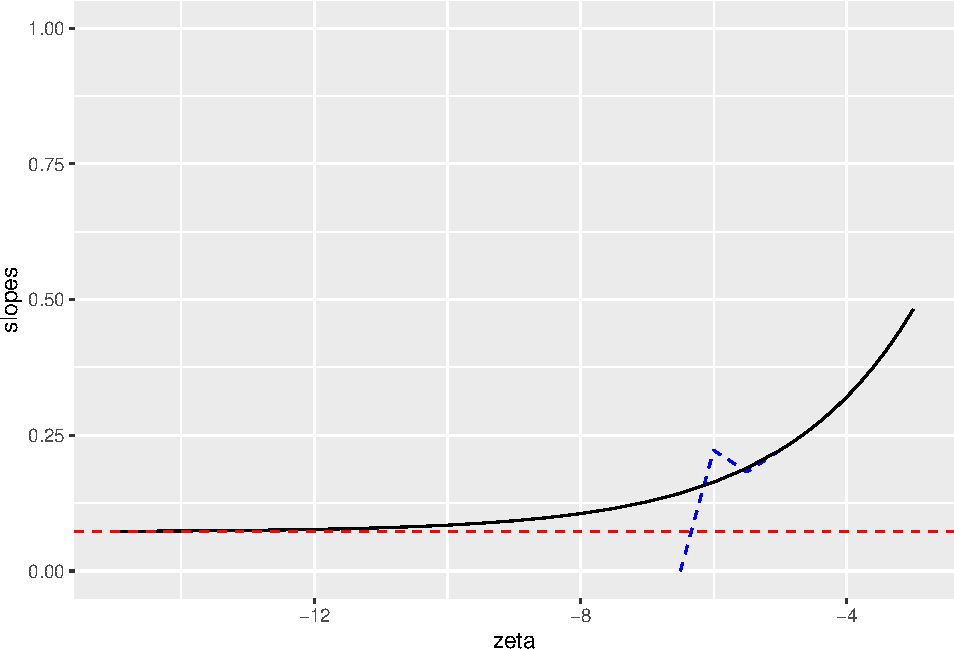
\includegraphics{07-rsm-predictions1_files/figure-latex/rsm-predictions-plots1-1.pdf}
\caption{\label{fig:rsm-predictions-plots1}Horizontal dashed red line: the value of \texttt{mStLine}, the slope of the straight line connecting the ROC end-point to (1,1). Dashed blue line: slope using double precision arithmetic. Solid black line: slope using multiple precision arithmetic - this curve approaches the limiting value \texttt{mStLine}.}
\end{figure}

The solid black line is the plot, using multiple precision arithmetic, of slope of the ROC curve vs.~\(\zeta\). The dashed blue line is the slope using standard precision arithmetic. The horizontal dashed red line is the slope of the straight line connecting the end-point to (1,1), i.e., 0.4935272. Standard precision arithmetic breaks down below \(\zeta \approx -6\) rapidly falling to illegal values \texttt{Nan} (above \(\zeta \approx -5\) there is little difference between standard and multiple precision). The multiple precision curve approaches the slope of the straight line as \(\zeta\) approaches -20. This confirms numerically the continuity of the slope of the ROC at the end-point.

\hypertarget{rsm-other-predictions}{%
\chapter{Other RSM predictions}\label{rsm-other-predictions}}

\hypertarget{rsm-other-predictions-how-much-finished}{%
\section{TBA How much finished}\label{rsm-other-predictions-how-much-finished}}

95\%
Work on intro
Need better word than constrained
finite? discontinuous? end-point-discontinuity?

\hypertarget{rsm-other-predictions-intro}{%
\section{TBA Introduction}\label{rsm-other-predictions-intro}}

Chapter \ref{empirical} described ROC, FROC, AFROC and wAFROC empirical plots and illustrated them using an actual FROC dataset. Chapter \ref{rsm-predictions} described the ROC curve and related quantities predicted by the radiological search model (RSM). This chapter describes the FROC, AFROC and wAFROC curve predictions of the RSM.

Use of a parametric model allows greater insight into the RSM predictions, for example the limiting slopes of the plots at the origin and the end-point, than is possible with empirical plots. Systematic variation of the parameters quantifies some of the expectations based on the solar analogy in Section \ref{froc-paradigm-solar-analogy}. This chapter also illustrates the need for using reasonable values of the parameters - this is achieved using the intrinsic \(\lambda_i, \nu_i\) parameters, described in Section \ref{rsm-intrinsic-parameters}. While the physical parameters \(\lambda, \nu\) are easier to understand as relate immediately to the FROC plot end-point, assigning arbitrary values to them can lead to unrealistic predictions.

\hypertarget{rsm-other-predictions-froc-curve}{%
\section{RSM-predicted FROC curve}\label{rsm-other-predictions-froc-curve}}

From a property of the Poisson distribution, namely its mean equals the \(\lambda\) parameter of the distribution, it follows that the expected number of \emph{latent} NLs per case is \(\lambda\). Recalling that NL z-samples are distributed as N(0,1), one multiplies \(\lambda\) by the probability that a z-sample from \(N(0,1)\) exceeds \(\zeta\), i.e.~by \(\Phi(-\zeta)\), to obtain the expected number of \emph{marked} NLs per case, i.e., NLF:

\begin{equation}
\text{NLF} \left ( \zeta, \lambda \right ) = \lambda \Phi \left (-\zeta \right )
\label{eq:rsm-other-predictions-nlf}
\end{equation}

We calculate \(\text{LLF}\) as follows:

\begin{equation} 
\left. 
\begin{aligned}
\text{LLF} \left ( \mu, \lambda, \nu, \overrightarrow{f_L} \right ) 
=& \Phi\left ( \mu - \zeta \right )\sum_{L=1}^{L_{max}} f_L \frac{1}{L} \sum_{l_2=0}^{L}  \, l_2 \,\,  \text{pmf}_{B}\left ( l_2, L, \nu \right )\\
=&\Phi\left ( \mu - \zeta \right )\sum_{L=1}^{L_{max}} f_L \frac{1}{L} L \,\nu\\
=&\nu \,\Phi\left ( \mu - \zeta \right )
\end{aligned}
\right \}
\label{eq:rsm-other-predictions-llf}
\end{equation}

The inner summation is over all cases with \(L\) lesions. One calculates the expected value of \(l_2\) (the number of lesions that are latent LLs) using the binomial distribution of \(l_2\); one divides by \(L\) to get the average fraction of LLs on cases with \(L\) lesions; one performs an average using the distribution \(f_L\) of cases with \(L\) lesions; since LL z-samples are distributed as \(N(\mu,1)\), one multiplies by the probability that a z-sample from \(N(\mu,1)\) exceeds \(\zeta\), i.e.~by \(\Phi(\mu-\zeta)\), to obtain the expected number of \emph{marked} LLs per case, i.e., LLF. Note that the final expression for LLF is independent of the number of lesions in the dataset or their distribution.

The coordinates of the RSM-predicted operating point on the FROC curve for threshold \(\zeta\) are given by Eqn. \eqref{eq:rsm-other-predictions-nlf} and Eqn. \eqref{eq:rsm-other-predictions-llf}. The FROC curve starts at (0,0) and ends at \(\left ( \lambda, \nu \right )\) -- the end-point. The end-point is not constrained to lie within the unit-square, rather it is \emph{semi-constrained}: while the maximum ordinate, i.e., \(\nu\), cannot exceed unity the maximum abscissa, i.e., \(\lambda\), can.

The clear connection between \(\lambda\) and \(\nu\) and the FROC end-point is the reason they are called the \emph{physical} RSM parameters. For reasons explained in Section \ref{froc-paradigm-solar-analogy} the physical parameters are not the best way of characterizing predicted RSM curves: they hide an inherent \(\mu\) dependence ignoring which can lead to unreasonable choices of RSM parameters (see Appendix \ref{rsm-other-predictions-froc-physical-parameters}). Intrinsic parameters \(\lambda_i, \nu_i\) were introduced in Section \ref{rsm-intrinsic-parameters} which are independent of \(\mu\). For convenience the transformations between physical and intrinsic parameters are reproduced here:

\begin{equation}
\left. 
\begin{aligned}
\nu =& 1 - \text{exp}\left ( - \mu \nu_i \right ) \\
\lambda =& \frac{\lambda_i}{\mu}
\end{aligned}
\right \}
\label{eq:rsm-other-predictions-transform}
\end{equation}

The predicted FROC, AFROC and wAFROC curves that follow use the intrinsic \(\lambda_i, \nu_i\) parameters.

\hypertarget{froc-plots-lambda_i-nu_i-parameterization}{%
\subsection{\texorpdfstring{FROC plots \(\lambda_i, \nu_i\) parameterization}{FROC plots \textbackslash lambda\_i, \textbackslash nu\_i parameterization}}\label{froc-plots-lambda_i-nu_i-parameterization}}

The following code generates FROC plots using the intrinsic \(\lambda_i = 2\) and \(\nu_i = 0.5\) parameters for 4 values of \(\mu\) contained in the array \texttt{muArr\ \textless{}-\ c(0.1,1,2,4)} (to avoid a divide by zero error the value \(\mu=0\) is not allowed). A \texttt{list} array \texttt{p\_FROC\_lambdai\_nui} is created to hold the four plots\footnote{Notation: \texttt{p\_} stands for a plot array, \texttt{FROC} stands for type of plot (also allowed are \texttt{AFROC} and \texttt{wAFROC}), \texttt{lambdai} stands for \(\lambda_i\) and \texttt{nui} stands for \(\nu_i\) (also allowed are \texttt{lambda} for \(\lambda\) and \texttt{nu} for \(\nu\) ).}. The intrinsic \(\lambda_i, \nu_i\) parameters are converted to \(\lambda, \nu\) using the function \texttt{Util2Physical()}which implements Eqn. \eqref{eq:rsm-other-predictions-transform}). The parameters are displayed using the \texttt{cat()} function. The plots are generated using \texttt{PlotRsmOperatingCharacteristics()}. Online help on this function is \href{https://dpc10ster.github.io/RJafroc/reference/PlotRsmOperatingCharacteristics.html}{available}. The code-line \texttt{p\_FROC\_lambdai\_nui{[}{[}i{]}{]}\ \textless{}-\ ret1\$FROCPlot} saves the plot to the previously created \texttt{list} array.

\begin{Shaded}
\begin{Highlighting}[]
\NormalTok{muArr }\OtherTok{\textless{}{-}} \FunctionTok{c}\NormalTok{(}\FloatTok{0.1}\NormalTok{,}\DecValTok{1}\NormalTok{,}\DecValTok{2}\NormalTok{,}\DecValTok{4}\NormalTok{)}
\NormalTok{lambda\_i }\OtherTok{\textless{}{-}} \DecValTok{2}
\NormalTok{nu\_i }\OtherTok{\textless{}{-}} \FloatTok{0.5}
\NormalTok{p\_FROC\_lambdai\_nui }\OtherTok{\textless{}{-}} \FunctionTok{array}\NormalTok{(}\FunctionTok{list}\NormalTok{(), }\AttributeTok{dim =} \FunctionTok{c}\NormalTok{(}\FunctionTok{length}\NormalTok{(muArr)))}
\ControlFlowTok{for}\NormalTok{ (i }\ControlFlowTok{in} \DecValTok{1}\SpecialCharTok{:}\FunctionTok{length}\NormalTok{(muArr)) \{}
\NormalTok{  mu }\OtherTok{\textless{}{-}}\NormalTok{ muArr[i]}
\NormalTok{  ret }\OtherTok{\textless{}{-}} \FunctionTok{Util2Physical}\NormalTok{(mu, }\AttributeTok{lambda\_i =}\NormalTok{ lambda\_i, }\AttributeTok{nu\_i =}\NormalTok{ nu\_i)}
\NormalTok{  lambda }\OtherTok{\textless{}{-}}\NormalTok{ ret}\SpecialCharTok{$}\NormalTok{lambda}
\NormalTok{  nu }\OtherTok{\textless{}{-}}\NormalTok{ ret}\SpecialCharTok{$}\NormalTok{nu}
  \FunctionTok{cat}\NormalTok{(}\FunctionTok{sprintf}\NormalTok{(}\StringTok{"lambda = \%6.3f, nu = \%4.3f"}\NormalTok{, lambda, nu), }\StringTok{"}\SpecialCharTok{\textbackslash{}n}\StringTok{"}\NormalTok{)}
\NormalTok{  ret1 }\OtherTok{\textless{}{-}} \FunctionTok{PlotRsmOperatingCharacteristics}\NormalTok{(}
\NormalTok{    mu, lambda, nu,}
    \AttributeTok{OpChType =} \StringTok{"FROC"}\NormalTok{,}
    \AttributeTok{legendPosition  =} \StringTok{"none"}\NormalTok{,}
    \AttributeTok{nlfRange =} \FunctionTok{c}\NormalTok{(}\DecValTok{0}\NormalTok{,}\DecValTok{4}\NormalTok{),}
    \AttributeTok{llfRange =} \FunctionTok{c}\NormalTok{(}\DecValTok{0}\NormalTok{,}\DecValTok{1}\NormalTok{)}
\NormalTok{  )}
\NormalTok{  p\_FROC\_lambdai\_nui[[i]] }\OtherTok{\textless{}{-}}\NormalTok{ ret1}\SpecialCharTok{$}\NormalTok{FROCPlot }
  \CommentTok{\#+ ggtitle(paste0("mu = ", as.character(muArr[i])))}
\NormalTok{\}}
\end{Highlighting}
\end{Shaded}

\begin{verbatim}
## lambda = 20.000, nu = 0.049 
## lambda =  2.000, nu = 0.393 
## lambda =  1.000, nu = 0.632 
## lambda =  0.500, nu = 0.865
\end{verbatim}

The following code displays the 4 plots.

\begin{Shaded}
\begin{Highlighting}[]
\FunctionTok{suppressWarnings}\NormalTok{(}\FunctionTok{grid.arrange}\NormalTok{(}
\NormalTok{p\_FROC\_lambdai\_nui[[}\DecValTok{1}\NormalTok{]],}
\NormalTok{p\_FROC\_lambdai\_nui[[}\DecValTok{2}\NormalTok{]],}
\NormalTok{p\_FROC\_lambdai\_nui[[}\DecValTok{3}\NormalTok{]],}
\NormalTok{p\_FROC\_lambdai\_nui[[}\DecValTok{4}\NormalTok{]], }\AttributeTok{ncol =} \DecValTok{2}\NormalTok{))}
\end{Highlighting}
\end{Shaded}

\begin{figure}
\centering
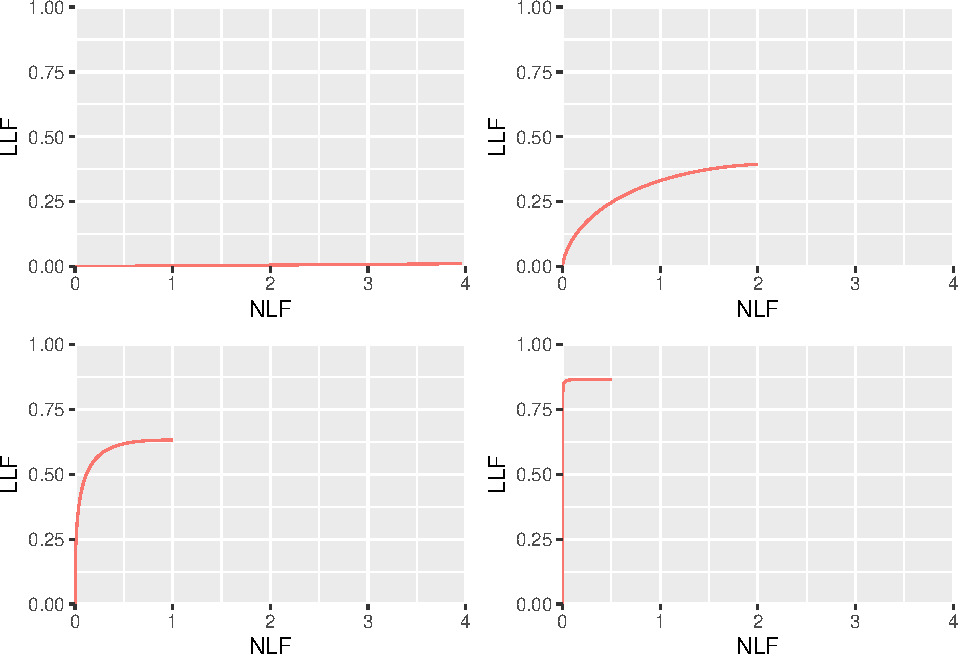
\includegraphics{08-rsm-predictions2_files/figure-latex/rsm-other-predictions-froc-plots-lambdai-nui-1.pdf}
\caption{\label{fig:rsm-other-predictions-froc-plots-lambdai-nui}RSM-predicted FROC curves using intrinsic parameters \(\lambda_i = 2\) and \(\nu_i = 0.5\). Top left: \(\mu = 0.1\); Top right: \(\mu = 1\); Bottom left: \(\mu = 2\); Bottom right: \(\mu = 4\). Some plots are \textbf{not} contained within the unit square which makes it impossible to use the FROC-AUC as a figure of merit.}
\end{figure}

\begin{quote}
\begin{itemize}
\tightlist
\item
  In the top-left plot (corresponding to \(\mu = 0.1\)) because \(\lambda = 20\) defines the end-point abscissa and \(\nu = 0.049\) defines the end-point ordinate, the FROC curve is close to the x-axis ending at \((20, 0.049)\). For small \(\mu\) this is close to the chance line FROC. Recall the solar analogy in Section \ref{froc-paradigm-solar-analogy}. When lesion contrast is low the search mechanism has little chance of finding lesions (leading to small LLF) and generates many NLs in attempting to do so (leading to large NLF).
\item
  Increasing \(\mu\) to 1 decreases \(\lambda\) to 2 and simultaneously increases \(\nu\) to 0.393. The new end-point \((2,0.393)\) is evident in the upper-right plot.
\item
  Further increase in \(\mu\) decreases the abscissa of the end-point and increases the ordinate and the end-point approaches the top-left corner of the FROC plot.
\item
  The perfect performance FROC curve is the vertical line connecting the origin to (0,1). It occurs when \(\mu = \infty\).
\item
  Since the FROC end-point is not constrained to lie within the unit square it is not possible, using the FROC-AUC, to defined a valid figure of merit.
\item
  Other characteristics of FROC curves (e.g., slopes at the origin and the end-point) and differences between intrinsic and physical parameterizations of this curve, are explored in Appendix \ref{rsm-other-predictions-froc-physical-parameters}.
\end{itemize}
\end{quote}

\hypertarget{rsm-other-predictions-froc-afroc-curve}{%
\section{RSM-predicted AFROC curve}\label{rsm-other-predictions-froc-afroc-curve}}

The AFROC x-coordinate is the same as the ROC x-coordinate and Eqn. \eqref{eq:rsm-predictions-fpf} applies. The AFROC y-coordinate is identical to the FROC y-coordinate and Eqn. \eqref{eq:rsm-other-predictions-llf} applies. Therefore:

\begin{equation}
\left. 
\begin{aligned}
&\text{FPF}\left (\zeta , \lambda\right ) = 1 - \text{exp}\left ( -\lambda \Phi\left ( -\zeta \right )  \right )\\
&\text{LLF}\left( \zeta, \mu, \nu \right) = \nu  \Phi \left ( \mu - \zeta \right )
\end{aligned}
\right \}
\label{eq:rsm-other-predictions-afroc}
\end{equation}

The end-point of the AFROC is defined by:

\begin{equation}
\left. 
\begin{aligned}
\text{FPF}_{\text{max}} =& 1 - \text{exp} \left ( -\lambda \right )\\
\text{LLF}_{\text{max}} =& \nu 
\end{aligned}
\right \}
\label{eq:rsm-other-predictions-afroc-end-point}
\end{equation}

Like the ROC the AFROC has the constrained end-point property (i.e., the end-point lies within the unit square) which makes its AUC a valid performance metric.

\hypertarget{afroc-plots-lambda_i-nu_i-parameterization}{%
\subsection{\texorpdfstring{AFROC plots \(\lambda_i, \nu_i\) parameterization}{AFROC plots \textbackslash lambda\_i, \textbackslash nu\_i parameterization}}\label{afroc-plots-lambda_i-nu_i-parameterization}}

Shown below are AFROC curves for the same parameter values used to demonstrate the preceding FROC curves.

\begin{figure}
\centering
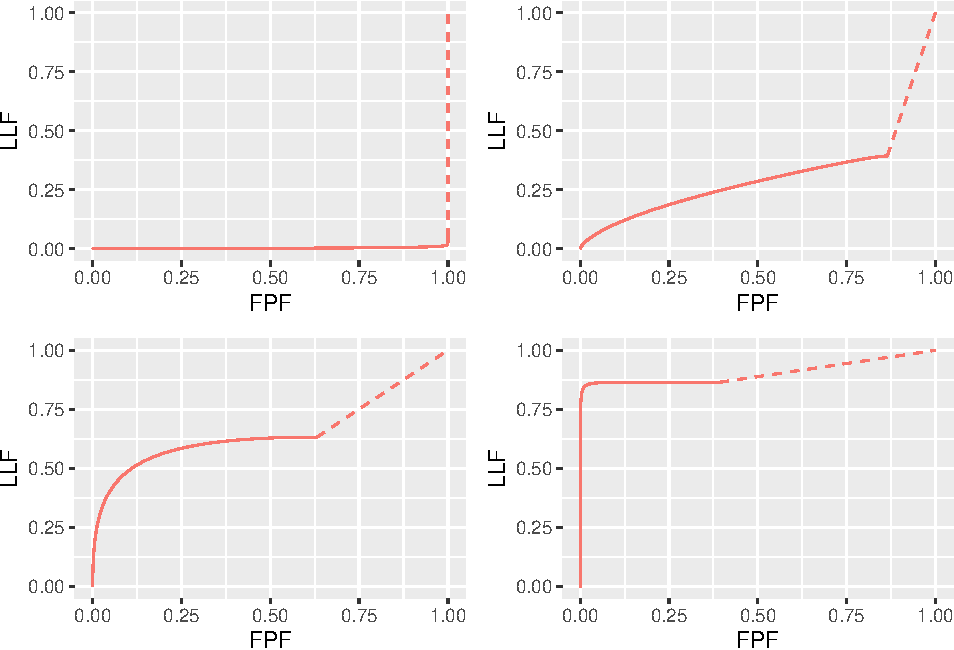
\includegraphics{08-rsm-predictions2_files/figure-latex/rsm-other-predictions-afroc-plots-lambdai-nui-1.pdf}
\caption{\label{fig:rsm-other-predictions-afroc-plots-lambdai-nui}RSM-predicted AFROC curves using intrinsic parameters \(\lambda_i = 2\) and \(\nu_i = 0.5\). Top left: \(\mu = 0.1\); Top right: \(\mu = 1\); Bottom left: \(\mu = 2\); Bottom right: \(\mu = 4\). Each curve includes an inaccessible dashed linear extension from the end-point to (1,1). Each plot is contained within the unit square and its AUC is a valid figure of merit.}
\end{figure}

\begin{quote}
\begin{itemize}
\tightlist
\item
  As discussed in the previous chapter for the ROC, each AFROC curve needs to be completed by a (dashed) straight line extending from the end-point to (1,1). A dashed line is used to distinguish it from the continous curve that is accessible to the observer by appropriate choice of \(\zeta\). The inaccessible dashed line is necessary to fully account for all decisions.
\item
  Since each plot is contained within the unit square its \emph{net} (i.e., continuous line plus dashed line) AUC is a valid performance metric.
\item
  The AFROC plot is independent of the number of lesions per case. This is not true for the wAFROC, as will shortly become clear, or the ROC (since the ROC ordinate increases with increasing numbers of lesions per case).
\item
  As \(\mu\) increases the AFROC curve more closely approaches the upper-left corner of the plot and the area under the AFROC curve, including that under the straight line extension, approaches 1, which is the best possible performance.
\item
  For \(\mu \to 0\) and fixed \(\lambda_i\) and \(\nu_i\) the operating characteristic approaches the horizontal line extending from the origin to (1,0), which is the continuous section of the curve, followed by the vertical dashed line connecting (1,0) to (1,1) and AFROC-AUC approaches zero. In this limit, no lesion is localized and every case has at least one NL mark, representing worst possible performance.
\item
  For \(\mu \to \infty\) the accessible portion of the operating characteristic approaches the vertical line connecting (0,0) to (0,1), the area under which is zero. The complete AFROC curve is obtained by connecting this point to (1,1) by the dashed line and in this limit the area under the complete ROC curve approaches 1. As with the ROC, omitting the area under the dashed portion of the curve will result in a severe underestimate of true performance.
\item
  Other characteristics of AFROC curves (e.g., slope and differences between intrinsic and physical parameterizations), are explored in Appendix \ref{rsm-other-predictions-afroc-physical-parameters}.
\end{itemize}
\end{quote}

\hypertarget{rsm-other-predictions-no-marks}{%
\subsection{Case of the reader who does not make any marks}\label{rsm-other-predictions-no-marks}}

Suppose the radiologist does not mark any case. One possibility is that the radiologist did not interpret the cases and simply ``whizzed'' through them. Even though the radiologist is not performing the diagnostic task and the AFROC operating point is stuck at the origin one would still be justified in making the straight-line extension to (1,1) which yields AFROC-AUC = 0.5, which implies finite performance (any value greater than zero for AFROC-AUC implies some degree of expertise). This is because the observer is correct in not marking any non-diseased case (any mark on such a case would be incorrect) and deserves credit for correct decisions on non-diseased cases. The situation is somewhat similar to an ROC study in which all cases are diagnosed as non-diseased - the observer is correct on all non-diseased cases and is rewarded with 100 percent specificity. However, the ROC-AUC for this observer is 0.5 (as the operating point is the origin and one needs to connect it via a dashed straight line to the upper right corner of the ROC plot) and the observer is operating at chance level performance, getting no credit for not marking non-diseased cases.

\hypertarget{rsm-other-predictions-wafroc-curve}{%
\section{RSM-predicted wAFROC curve}\label{rsm-other-predictions-wafroc-curve}}

The wAFROC abscissa is identical to the ROC abscissa, i.e., Eqn. \eqref{eq:rsm-predictions-fpf} applies. The wAFROC ordinate is calculated using:

\begin{equation} 
\text{wLLF} \left ( \mu, \lambda, \nu, \overrightarrow{f_L}, \mathbf{W} \right ) = \Phi\left ( \mu - \zeta \right )\sum_{L=1}^{L_{max}} f_L \sum_{l_2=1}^{L} \text{W}_{Ll_2} \, l_2 \,\,  \text{pmf}_{B}\left ( l_2, L, \nu \right )
\label{eq:rsm-other-predictions-wllf}
\end{equation}

Note that one does not divide by \(L\) outside the inner summation as, for each value of \(L\), the weights are already normalized to sum to unit: \(\sum_{l_2=1}^{L} \text{W}_{Ll_2}=1\).

Eqn. \eqref{eq:rsm-other-predictions-wllf} is implemented in \texttt{UtilAnalyticalAucsRSM}. Help is available \href{https://dpc10ster.github.io/RJafroc/reference/UtilAnalyticalAucsRSM.html}{here}. A skeleton code is shown below:

\begin{verbatim}
W <-UtilLesWghtsLD(lesDistr, relWeights)
wLLF <- 0
for (L in 1:L_max){
  wLLF_L <- 0
  for (l_2 in 1:L){
    # W has an extra column that must be skipped, hence W[L, l_2+1]
    wLLF_L <- wLLF_L + W[L, l_2+1] * l_2 * dbinom(l_2, L, nu)
  }
  wLLF <- wLLF +  f_L[L] * wLLF_L
}
wLLF <- wLLF * pnorm(mu - zeta)
\end{verbatim}

\begin{itemize}
\tightlist
\item
  \(\overrightarrow{f_L}\) is the normalized histogram of the lesion distribution for the diseased cases. In the software it is denoted \texttt{lesDistr}. For example, the array \texttt{lesDistr\ =\ c(0.1,\ 0.4,\ 0.4,\ 0.1)} defines a dataset in which 10 percent of the cases contain one lesion, 40 percent contain 2 lesions, 40 percent contain 3 lesions and 10 percent contain 4 lesions.
\item
  \(L_{max}\) is the maximum number of lesions per case in the dataset. In the preceding example \(L_{max} = 4\).
\item
  \(\mathbf{W}\) is the (lower triangular) square weights matrix with \(L_{max}\) rows and columns, where each row (excluding cells set to \(-\infty\)) sums to unity, see example below (the unused matrix elements are set to \(-\infty\)). In Eqn. \eqref{eq:rsm-other-predictions-wllf} the index \(l_2\) in \(W_{Ll_2}\) ranges from 1 to L.
\item
  The relative lesion weights are denoted in the code \texttt{relWeights}. For example, \texttt{relWeights\ =\ \ c(0.2,\ 0.3,\ 0.1,\ 0.5)} whose meaning is as follows:

  \begin{itemize}
  \tightlist
  \item
    On cases with one lesion the lesion weight is unity.
  \item
    On cases with two lesions the relative weights are 0.2 and 0.3. Since these do not add up to unity, the actual weights are 0.4 and 0.6.
  \item
    On cases with three lesions the relative weights are 0.2, 0.3 and 0.1. The actual weights are 1/3, 1/2 and 1/6.
  \item
    On cases with four lesions the relative weights are 0.2, 0.3, 0.1 and 0.5. The actual weights are 0.2, 0.3, 0.1 and 0.4.
  \end{itemize}
\item
  The function \texttt{UtilLesWghtsLD} calculates the matrix given \texttt{lesDistr} and \texttt{relWeights}. For example:
\end{itemize}

\begin{Shaded}
\begin{Highlighting}[]
\NormalTok{lesDistr }\OtherTok{\textless{}{-}} \FunctionTok{c}\NormalTok{(}\FloatTok{0.6}\NormalTok{, }\FloatTok{0.2}\NormalTok{, }\FloatTok{0.1}\NormalTok{, }\FloatTok{0.1}\NormalTok{)}
\NormalTok{relWeights }\OtherTok{=}  \FunctionTok{c}\NormalTok{(}\FloatTok{0.2}\NormalTok{, }\FloatTok{0.3}\NormalTok{, }\FloatTok{0.1}\NormalTok{, }\FloatTok{0.4}\NormalTok{)}
\FunctionTok{UtilLesWghtsLD}\NormalTok{(lesDistr, relWeights)[,}\SpecialCharTok{{-}}\DecValTok{1}\NormalTok{]}
\end{Highlighting}
\end{Shaded}

\begin{verbatim}
##           [,1] [,2]      [,3] [,4]
## [1,] 1.0000000 -Inf      -Inf -Inf
## [2,] 0.4000000  0.6      -Inf -Inf
## [3,] 0.3333333  0.5 0.1666667 -Inf
## [4,] 0.2000000  0.3 0.1000000  0.4
\end{verbatim}

\begin{itemize}
\tightlist
\item
  It is necessary to label the lesions properly so that the correct weights are used. This is done using the \texttt{lesionID} field in the Excel input file. For example, \texttt{lesionID\ =\ 3} for the one with relative weight 0.1. Since \(\mathbf{W}\) is independent of cases, the lesion characteristics (which determine outcome/importance) of the lesion with \texttt{lesionID\ =\ 1} in cases with one lesion or in cases with 4 lesions are identical. In other words this example assumes that the lesions fall into four classes, with clinical outcomes as specified in \texttt{relWeights}.
\item
  \(\text{pmf}_{B}\left ( l_2, L, \nu \right )\) is the probability mass function (pmf) of the binomial distribution with success probability \(\nu\) and trial size \(L\). \(\text{W}_{Ll_2}\) is the weight of lesion \(l_2\) in cases with \(L\) lesions; for example \(\text{W}_{42} = 0.3\).
\item
  To generate equal weights set \texttt{relWeights\ =\ 0} as in following code:
\end{itemize}

\begin{Shaded}
\begin{Highlighting}[]
\NormalTok{lesDistr }\OtherTok{\textless{}{-}} \FunctionTok{c}\NormalTok{(}\FloatTok{0.6}\NormalTok{, }\FloatTok{0.2}\NormalTok{, }\FloatTok{0.1}\NormalTok{, }\FloatTok{0.1}\NormalTok{)}
\NormalTok{relWeights0 }\OtherTok{\textless{}{-}} \DecValTok{0}
\FunctionTok{UtilLesWghtsLD}\NormalTok{(lesDistr, }\AttributeTok{relWeights =}\NormalTok{ relWeights0)[,}\SpecialCharTok{{-}}\DecValTok{1}\NormalTok{]}
\end{Highlighting}
\end{Shaded}

\begin{verbatim}
##           [,1]      [,2]      [,3] [,4]
## [1,] 1.0000000      -Inf      -Inf -Inf
## [2,] 0.5000000 0.5000000      -Inf -Inf
## [3,] 0.3333333 0.3333333 0.3333333 -Inf
## [4,] 0.2500000 0.2500000 0.2500000 0.25
\end{verbatim}

\hypertarget{wafroc-plots-lambda_i-nu_i-parameterization}{%
\subsection{\texorpdfstring{wAFROC plots \(\lambda_i, \nu_i\) parameterization}{wAFROC plots \textbackslash lambda\_i, \textbackslash nu\_i parameterization}}\label{wafroc-plots-lambda_i-nu_i-parameterization}}

\begin{quote}
\begin{itemize}
\tightlist
\item
  Shown below are wAFROC curves for the same parameter values used to display the AFROC curves shown in Fig. \ref{fig:rsm-other-predictions-afroc-plots-lambda-nu}.
\item
  Note that it is necessary to specify \texttt{lesDistr} when requesting a wAFROC plot. A dataset with a maximum of 4 lesions per diseased case is assumed, with \texttt{lesDistr\ \textless{}-\ c(0.6,\ 0.2,\ 0.1,\ 0.1)}.
\end{itemize}
\end{quote}

\begin{Shaded}
\begin{Highlighting}[]
\NormalTok{p\_wAFROC\_lambdai\_nui }\OtherTok{\textless{}{-}} \FunctionTok{array}\NormalTok{(}\FunctionTok{list}\NormalTok{(), }\AttributeTok{dim =} \FunctionTok{c}\NormalTok{(}\FunctionTok{length}\NormalTok{(muArr)))}
\ControlFlowTok{for}\NormalTok{ (i }\ControlFlowTok{in} \DecValTok{1}\SpecialCharTok{:}\FunctionTok{length}\NormalTok{(muArr)) \{}
\NormalTok{  mu }\OtherTok{\textless{}{-}}\NormalTok{ muArr[i]}
\NormalTok{  ret }\OtherTok{\textless{}{-}} \FunctionTok{Util2Physical}\NormalTok{(mu, }\AttributeTok{lambda\_i =}\NormalTok{ lambda\_i, }\AttributeTok{nu\_i =}\NormalTok{ nu\_i)}
\NormalTok{  lambda }\OtherTok{\textless{}{-}}\NormalTok{ ret}\SpecialCharTok{$}\NormalTok{lambda  }
\NormalTok{  nu }\OtherTok{\textless{}{-}}\NormalTok{ ret}\SpecialCharTok{$}\NormalTok{nu}
\NormalTok{  ret1 }\OtherTok{\textless{}{-}} \FunctionTok{PlotRsmOperatingCharacteristics}\NormalTok{(}
\NormalTok{    mu, lambda, nu,}
    \AttributeTok{lesDistr =}\NormalTok{ lesDistr,}
    \AttributeTok{relWeights =}\NormalTok{ relWeights,}
    \AttributeTok{OpChType =} \StringTok{"wAFROC"}\NormalTok{,}
    \AttributeTok{legendPosition  =} \StringTok{"none"}
\NormalTok{  )}
\NormalTok{  p\_wAFROC\_lambdai\_nui[[i]] }\OtherTok{\textless{}{-}}\NormalTok{ ret1}\SpecialCharTok{$}\NormalTok{wAFROCPlot }
  \CommentTok{\#+ ggtitle(paste0("mu = ", as.character(muArr[i]), }
  \CommentTok{\#+ ", AUC = ", format(ret1$aucAFROC, digits = 3)))}
\NormalTok{\}}
\end{Highlighting}
\end{Shaded}

\begin{figure}
\centering
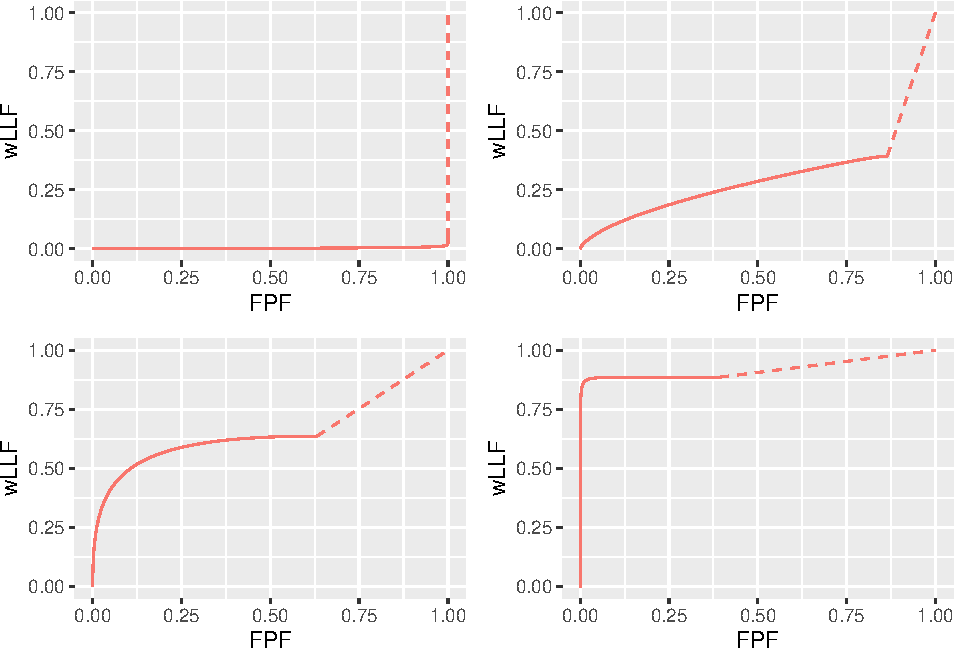
\includegraphics{08-rsm-predictions2_files/figure-latex/rsm-other-predictions-wafroc-plots-lambdai-nui-1.pdf}
\caption{\label{fig:rsm-other-predictions-wafroc-plots-lambdai-nui}RSM-predicted wAFROC curves using intrinsic parameters \(\lambda_i = 2\) and \(\nu_i = 0.5\). Top left: \(\mu = 0.1\). Top right: \(\mu = 1\). Bottom left: \(\mu = 2\). Bottom right: \(\mu = 4\). As \(\mu\) increases the curve approaches the top-left corner. Each curve includes an inaccessible dashed linear extension to (1,1). Since the plot is contained within the unit square its AUC is a valid figure of merit.}
\end{figure}

\hypertarget{rsm-other-predictions-comments}{%
\section{Comments on end-point-discontinuity property}\label{rsm-other-predictions-comments}}

RSM predicted ROC, AFROC and wAFROC curves share the end-point-discontinuity property (not extending continuously to (1,1)) that makes them qualitatively different from predictions of all other observer performance models that I am aware of. In my experience this is a property that most researchers in this field have difficulty with. There is simply too much history going back to the early 1940s of the ROC curve extending continuously from (0,0) to (1,1).

I am not aware of any empirical evidence that observers can actually operate \emph{continuously} in the range (0,0) to (1,1) \emph{in search tasks}, so the existence of such an ROC is an assumption. In contrast the ROC of an (algorithmic) observer in a \emph{non-search task} can extend continuously to (1,1). Consider a diagnostic test that rates the results of a laboratory measurement, e.g., the A1C measure of blood glucose for presence of a disease. If \(A1C \ge 0.065\) the patient is diagnosed as diabetic. By moving the threshold from \(+\infty\) to \(-\infty\), and assuming a large population of patients, one can trace out the entire ROC curve from the origin to (1,1). \emph{This is because every patient yields an A1C value.} Now imagine that some finite fraction of the test results are ``lost in the mail''; then the ROC curve, calculated over all patients, will have the end-point-discontinuity property, albeit due to an unreasonable cause.

The situation in medical imaging involving search tasks is more realistic. \emph{Not every case yields a decision variable.} There is a reasonable cause for this -- to render a decision variable sample the radiologist must find something suspicious to report, and if none is found, there is no decision variable to report. The ROC curve calculated over all patients would exhibit the end-point-discontinuity property, even in the limit of an infinite number of patients. If calculated over only those patients that yielded at least one mark, the ROC curve would extend from (0,0) to (1,1) but then one would be ignoring all cases with no marks. For non-diseased cases these represent correct decisions and for diseased cases they represent incorrect decisions and ignoring all cases with no marks should raise concern regarding validity of the analysis.

\hypertarget{rsm-other-predictions-appendix}{%
\section{Appendix}\label{rsm-other-predictions-appendix}}

Unlike the previous plots which used the \emph{intrinsic} parameters \(\lambda_i, \nu_i\), the plots shown here are for arbitrary choices of RSM \emph{physical} parameters \(\lambda, \nu\). This can lead to peculiar predictions arising from physically unreasonable parameter values.

\hypertarget{rsm-other-predictions-froc-physical-parameters}{%
\subsection{Slope of the FROC curve}\label{rsm-other-predictions-froc-physical-parameters}}

Expressions for LLF and NLF were given above. Taking the derivatives of these functions with respect to \(\zeta\) the slope of the FROC is given by:

\begin{equation}
\left. 
\begin{aligned}
\frac{\frac{\partial }{\partial \zeta}\left( LLF \right)}{\frac{\partial }{\partial \zeta}\left( NLF \right)}  
=& \frac{\nu}{\lambda}  \frac{\phi\left( \mu-\zeta \right)}{\phi\left( -\zeta \right)} \\
\end{aligned}
\right \} 
\label{eq:rsm-other-predictions-froc-slope1}
\end{equation}

With some simplification this yields:

\begin{equation}
\left. 
\begin{aligned}
\frac{\frac{\partial }{\partial \zeta}\left( LLF \right)}{\frac{\partial }{\partial \zeta}\left( NLF \right)}  
=& \frac{\nu}{\lambda}  \frac{\text{exp}\left ( \frac{-\left (\mu-\zeta  \right )^2}{2} \right )}{\text{exp}\left ( \frac{-\zeta^2}{2} \right )} \\
=& \frac{\nu}{\lambda} \text{exp}\left (-\frac{1}{2} \left( \mu^2 - 2\mu\zeta \right)\right ) \\
\end{aligned}
\right \} 
\label{eq:rsm-other-predictions-froc-slope2}
\end{equation}

Converting to intrinsic parameters leads to the following expression for the slope:

\begin{equation}
\left. 
\begin{aligned}
\frac{\frac{\partial }{\partial \zeta}\left( LLF \right)}{\frac{\partial }{\partial \zeta}\left( NLF \right)}  
=& \mu \left( \frac{1 - \text{exp}\left ( - \mu \nu_i \right ) }{\lambda_i} \right) \text{exp}\left (-\frac{1}{2} \left( \mu^2 - 2\mu\zeta \right)  \right )
\end{aligned}
\right \} 
\label{eq:rsm-other-predictions-froc-slope3}
\end{equation}

Eqn. \eqref{eq:rsm-other-predictions-froc-slope3} leads to the following conclusions (recall \(\mu \ge 0\)):

\begin{quote}
\begin{itemize}
\tightlist
\item
  The slope of the FROC near the end-point, corresponding to \(\zeta = -\infty\), is zero.
\item
  The slope near the origin, corresponding to \(\zeta = +\infty\), is \(\infty\) provided \(\mu \ne 0\).
\item
  For \(\mu = 0\) the slope of the FROC is zero regardless of the value of \(\zeta\), see top-left panel in Fig. \ref{fig:rsm-other-predictions-froc-plots-lambdai-nui}.
\end{itemize}
\end{quote}

If instead we had used Eqn. \eqref{eq:rsm-other-predictions-froc-slope2} the last conclusion would change to:

\begin{quote}
\begin{itemize}
\tightlist
\item
  For \(\mu = 0\) the FROC is predicted to be a straight line extending from the origin to \((\lambda, \nu)\), as in the top-left plot in Fig. \ref{fig:rsm-other-predictions-froc-plots-lambda-nu} corresponding to \(\mu=0\), \(\lambda = 1\) and \(\nu = 0.2\). This is unreasonable since for zero contrast lesions the observer should not be able to localize any lesions at finite NLF. The unreasonable prediction is occurring because one is using unrealistic values for the RSM parameters. For zero \(\mu\) one expects \(\lambda = \infty\) and \(\nu = 0\), not \(\lambda = 1\) and \(\nu = 0.2\).
\end{itemize}
\end{quote}

\hypertarget{froc-plots-lambda-nu-parameterization}{%
\subsection{\texorpdfstring{FROC plots \(\lambda, \nu\) parameterization}{FROC plots \textbackslash lambda, \textbackslash nu parameterization}}\label{froc-plots-lambda-nu-parameterization}}

FROC plots are shown below illustrating the statements just made.

\begin{verbatim}
## mu =  0.100, lambda =  1.000, nu = 0.200 
## mu =  1.000, lambda =  2.000, nu = 0.500 
## mu =  2.000, lambda =  3.000, nu = 0.700 
## mu =  4.000, lambda =  4.000, nu = 0.900
\end{verbatim}

\begin{figure}
\centering
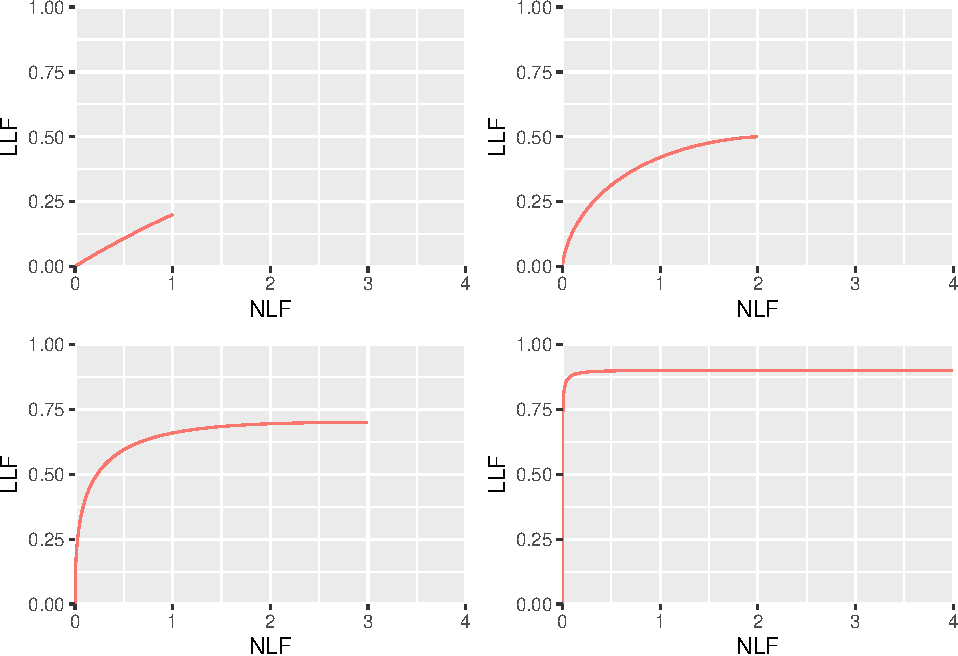
\includegraphics{08-rsm-predictions2_files/figure-latex/rsm-other-predictions-froc-plots-lambda-nu-1.pdf}
\caption{\label{fig:rsm-other-predictions-froc-plots-lambda-nu}RSM-predicted FROC curves using \(\lambda, \nu\) paramterization. Top left: \(\mu = 0.1\), \(\lambda = 1\) and \(\nu = 0.2\). Top right: \(\mu = 1\), \(\lambda = 2\) and \(\nu = 0.5\). Bottom left: \(\mu = 2\), \(\lambda = 3\) and \(\nu = 0.7\). Bottom right: \(\mu = 4\), \(\lambda = 4\) and \(\nu = 0.9\). The top-left panel is an unrealistic prediction because of unrealistic parameters \(\lambda =1, \nu = 0.2\) for small \(\mu\).}
\end{figure}

\hypertarget{rsm-other-predictions-afroc-physical-parameters}{%
\subsection{Slope of the AFROC curve}\label{rsm-other-predictions-afroc-physical-parameters}}

The AFROC ordinate is LLF and the abscissa is FPF. Expressions for both were given above. Taking the derivatives of these functions with respect to \(\zeta\) the slope of the continuous section of the AFROC is given by:

\begin{equation}
\left. 
\begin{aligned}
\frac{\frac{\partial }{\partial \zeta}\left( LLF \right)}{\frac{\partial }{\partial \zeta}\left( FPF \right)} 
=& \frac{\nu \phi \left ( \mu-\zeta \right )}{\text{exp}\left( -\lambda \Phi\left(- \zeta \right)\left( \lambda\phi\left( -\zeta \right)  \right) \right)} 
\end{aligned}
\right \} 
\label{eq:rsm-other-predictions-afroc-slope}
\end{equation}

Using Eqn. \eqref{eq:rsm-other-predictions-froc-slope1} the slope of the AFROC can be expressed in terms of the slope of the FROC:

\begin{equation}
\left. 
\begin{aligned}
\frac{\frac{\partial }{\partial \zeta}\left( LLF \right)}{\frac{\partial }{\partial \zeta}\left( FPF \right)} 
=& \frac{\frac{\frac{\partial }{\partial \zeta}\left( LLF \right)}{\frac{\partial }{\partial \zeta}\left( NLF \right)}}{\text{exp}\left ( -\lambda \Phi\left ( -\zeta \right )  \right )}\\ 
=& \frac{\frac{\frac{\partial }{\partial \zeta}\left( LLF \right)}{\frac{\partial }{\partial \zeta}\left( NLF \right)}}{1-FPF\left( \lambda, \zeta \right)}\\ 
\end{aligned}
\right \} 
\label{eq:rsm-other-predictions-afroc-slope3}
\end{equation}

The numerator is the slope of the FROC. Since \(0 \le \text{FPF} \le \text{FPF}_{\text{max}}\) and \(\text{FPF}\) increases as \(\zeta\) decreases, the slope of the AFROC equals that of the FROC at the origin and subsequently increases over that of the FROC as the end-point is approached.

This expression leads to the following conclusions, if using intrinsic parameterization:

\begin{quote}
\begin{itemize}
\tightlist
\item
  The slope of the AFROC near the end-point, corresponding to \(\zeta = -\infty\), is zero provided \(\mu \ne 0\).
\item
  The slope near the origin, corresponding to \(\zeta = +\infty\), is \(\infty\) provided \(\mu \ne 0\).
\item
  For \(\mu = 0\) the slope of the AFROC is zero regardless of the value of \(\zeta\), see top-left panel in Fig. \ref{fig:rsm-other-predictions-afroc-plots-lambdai-nui}.
\end{itemize}
\end{quote}

If using physical parameters the last conclusion changes to:

\begin{quote}
\begin{itemize}
\tightlist
\item
  For \(\mu = 0\) the slope of the AFROC curve increases as the end-point is approached, i.e., the FROC curve is concave up, see top-left panel in Fig. \ref{fig:rsm-other-predictions-afroc-plots-lambda-nu}. The unreasonable prediction is due to the unreasonable choice of parameters.
\end{itemize}
\end{quote}

\begin{verbatim}
## mu =  0.100, lambda =  1.000, nu = 0.200 
## mu =  1.000, lambda =  2.000, nu = 0.500 
## mu =  2.000, lambda =  3.000, nu = 0.700 
## mu =  4.000, lambda =  4.000, nu = 0.900
\end{verbatim}

\begin{figure}
\centering
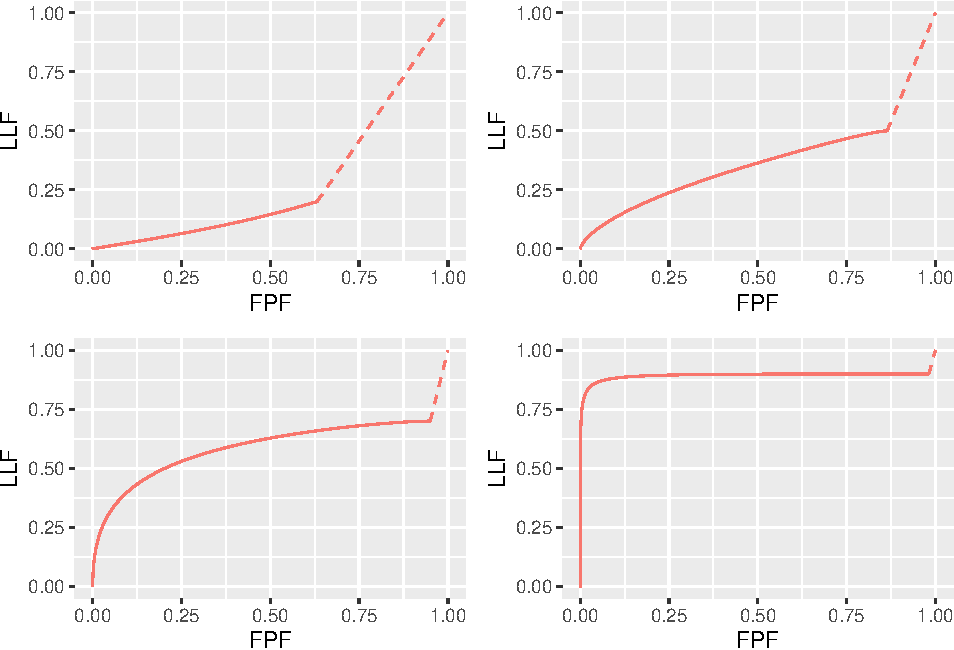
\includegraphics{08-rsm-predictions2_files/figure-latex/rsm-other-predictions-afroc-plots-lambda-nu-1.pdf}
\caption{\label{fig:rsm-other-predictions-afroc-plots-lambda-nu}RSM-predicted AFROC curves, \(\lambda, \nu\) paramterization, using same parameter choices as in preceding plot. Note the unrealistic concave up feature of the top-left plot due to unrealistic choices of parameters.}
\end{figure}

\hypertarget{rsm-other-predictions-wafroc-physical-parameters}{%
\subsection{\texorpdfstring{wAFROC plots \(\lambda, \nu\) parameterization}{wAFROC plots \textbackslash lambda, \textbackslash nu parameterization}}\label{rsm-other-predictions-wafroc-physical-parameters}}

\begin{verbatim}
## mu =  0.100, lambda =  1.000, nu = 0.200 
## mu =  1.000, lambda =  2.000, nu = 0.500 
## mu =  2.000, lambda =  3.000, nu = 0.700 
## mu =  4.000, lambda =  4.000, nu = 0.900
\end{verbatim}

\begin{figure}
\centering
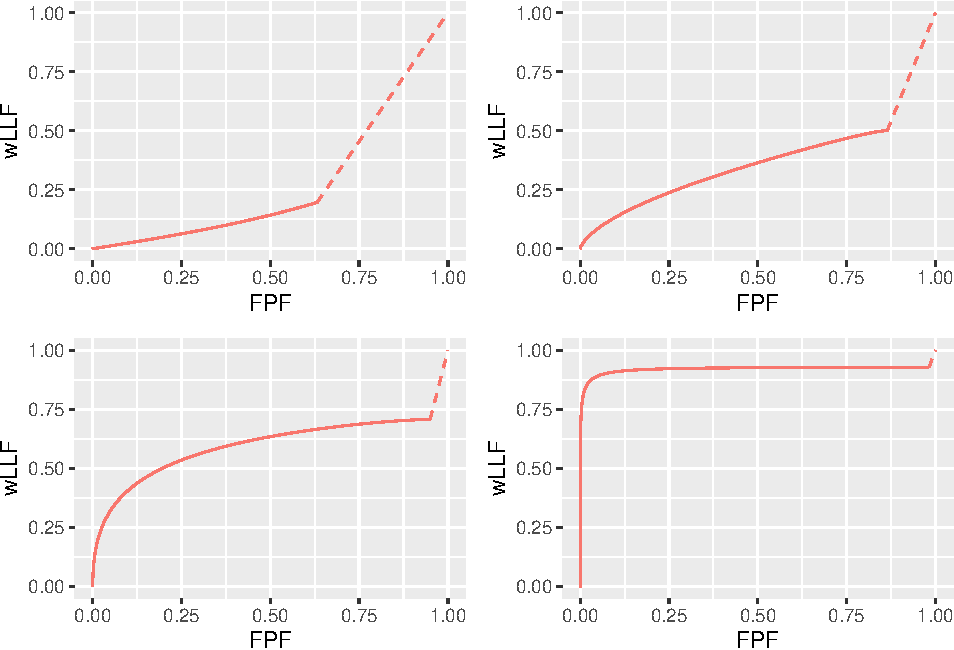
\includegraphics{08-rsm-predictions2_files/figure-latex/rsm-other-predictions-wafroc-plots-lambda-nu-1.pdf}
\caption{\label{fig:rsm-other-predictions-wafroc-plots-lambda-nu}RSM-predicted wAFROC curves, \(\lambda, \nu\) paramterization, using same parameter choices as in preceding plot. Note the unrealistic concave up feature of the top-left plot due to unrealistic choices of parameters.}
\end{figure}

\hypertarget{rsm-other-predictions-roc-above-afroc}{%
\subsection{ROC curves are above AFROC curves}\label{rsm-other-predictions-roc-above-afroc}}

Since they share a common x-axis one can compare the relative position of ROC and AFROC curves for the same parameter values, i.e., does one lie above or below the other. Using previous equations for the ROC-TPF and the AFROC-LLF, and focusing on cases with \(L\) lesions, one has:

\begin{equation}
\left.
\begin{aligned}
& \text{TPF}-\text{LLF} \\
&= 1 - \text{exp}\left ( - \lambda \Phi \left ( - \zeta \right )\right )
\left ( 1 - \nu \Phi \left ( \mu - \zeta \right ) \right )^L - \nu  \Phi \left ( \mu - \zeta \right )\\
&= 1 - \nu  \Phi \left ( \mu - \zeta \right )- \text{exp}\left ( - \lambda \Phi \left ( - \zeta \right )\right )
\left ( 1  - \nu \Phi \left ( \mu - \zeta \right ) \right )^L \\
&= \left( 1 - \nu  \Phi \left ( \mu - \zeta \right ) \right)\left[ 1 - \text{exp}\left ( - \lambda \Phi \left ( - \zeta \right )\right ) 
\left ( 1  - \nu \Phi \left ( \mu - \zeta \right ) \right )^{L-1}  \right]\\
& \ge0
\end{aligned}
\right \}
\label{eq:rsm-predictions-roc-above-afroc}
\end{equation}

The final inequality follows from the facts that:

\begin{itemize}
\tightlist
\item
  \(1 - \nu \Phi \left ( \mu - \zeta \right )\) is non-negative and less than or equal to one, and so are any integer powers of this quantity.
\item
  \(\text{exp}\left ( - \lambda \Phi \left ( - \zeta \right )\right )\) is non-negative and less than or equal to one.
\item
  The equality is achieved when \(\zeta = +\infty\), i.e., at the origin (since the \(\Phi\) function evaluates to zero).
\item
  Averaging over \(f_L\), the distribution of lesions, does not change the final conclusion.
\end{itemize}

\begin{quote}
The basic reason why TPF is greater than LLF is that the ROC gives credit for incorrect localizations on diseased cases while the AFROC does not. This is the well-known ``right for wrong reason'' argument \citep{bunch1977free}, originally advanced in 1977, against usage of the ROC for localization tasks.
\end{quote}

\hypertarget{rsm-other-predictions-wafroc-above-afroc}{%
\subsection{Are wAFROC curves above AFROC curves?}\label{rsm-other-predictions-wafroc-above-afroc}}

The following expression follows for the difference between wLLF and LLF:

\begin{equation} 
\left.
\begin{aligned}
\text{wLLF}-\text{LLF}
= \Phi\left ( \mu - \zeta \right )\sum_{L=1}^{L_{max}} f_L  \sum_{l_2=1}^{L} \left( \text{W}_{Ll_2} -\frac{1}{L} \right) \, l_2 \,\,  \text{pmf}_{B}\left ( l_2, L, \nu \right )
\end{aligned}
\right \}
\label{eq:rsm-other-predictions-wllf-llf}
\end{equation}

Since for equally weighted lesions each lesion weight is \(\frac{1}{L}\), this equation shows immediately that for equally weighted lesions the difference is zero, i.e., \emph{for equally weighted lesions the wAFROC and the AFROC are identical}:

\begin{equation} 
\left| \text{wLLF} \right|_\text{equal weights} -\text{LLF} = 0
\label{eq:rsm-other-predictions-wllf-llf-eq-weights}
\end{equation}

In the general case the two curves are not identical although, for realistic datasets, the differences tend to be small. For cases with L lesions the probability mass function of the binomial distribution is peaked near \(l_2 =L\nu\). If the weights array \(W_{Ll_2}\) is likewise peaked near \(l_2 =L\nu\) the difference tends to be positive, i.e., the wAFROC is above the AFROC. Otherwise the difference can be negative.

\hypertarget{rsm-search-classification}{%
\chapter{Lesion localization and classification performances}\label{rsm-search-classification}}

\hypertarget{rsm-search-classification-how-much-finished}{%
\section{How much finished}\label{rsm-search-classification-how-much-finished}}

99\%

\hypertarget{rsm-search-classification-intro}{%
\section{Introduction}\label{rsm-search-classification-intro}}

The preceding two chapters described predictions of the radiological search model (RSM). This chapter describes two performance measures, namely \emph{lesion-localization and lesion-classification performances}, that can be derived from the predicted ROC. These performances were introduced conceptually in Section \ref{visual-search-search-classification} and this chapter deals with relating them to the RSM parameters.

Recall the the search process involves two stages: (1) finding suspicious regions and (2) correctly classifying each suspicious region as either a lesion (in which case the region is marked and rated) or a non-lesion (in which case the region is not marked). The first stage is the lesion-localization task while the second stage is the lesion-classification task. Performance in the lesion-localization task is measured by the ability to mark lesions while minimizing marking non-lesions. Performance in the classification task is the ability, having found a suspicious region, to correctly recognize it as a lesion (to be marked and rated) or a non-lesion (to be ignored). The aim of this chapter is to quantify these two abilities.

\hypertarget{rsm-search-classification-quantifying}{%
\section{Quantifying lesion-localization performance}\label{rsm-search-classification-quantifying}}

From Chapter \ref{rsm-predictions} the coordinates of the RSM-predicted ROC end-point are given by:

\begin{equation}
\left. 
\begin{aligned}
&\text{FPF}_{\text{max}} = 1 - \text{exp}\left (\lambda \right ) \\
&\text{TPF}_{\text{max}} = 1 - \text{exp} \left ( - \lambda \right )\sum_{L=1}^{L_{max}}f_L \left ( 1 - \nu \right )^L
\end{aligned}
\right \}
\label{eq:rsm-search-classification-FPF-TPF-max}
\end{equation}

Qualitatively, lesion-localization performance is the ability to mark lesions while not marking non-lesions. To arrive at a quantitative definition consider the location of the ROC end-point.

In Fig. \ref{fig:rsm-search-classification-performance-from-roc-curve} curve (a) is a typical ROC curve predicted by models that do not account for lesion-localization, specifically the binormal model is considered here. The corresponding end-point is at (1,1), the filled circle, i.e., by adopting a sufficiently low reporting threshold the observer can continuously move the operating point to (1,1). The curve labeled (b) is a typical RSM-predicted ROC curve. The corresponding end-point, the filled square, is downwards and left shifted relative to (1,1). The chance diagonal is the straight line labeled (c).

The specific parameter values used in the illustration are shown next:

\begin{Shaded}
\begin{Highlighting}[]
\NormalTok{a }\OtherTok{\textless{}{-}} \DecValTok{2}\NormalTok{; b }\OtherTok{\textless{}{-}} \DecValTok{1} \CommentTok{\# binormal model}
\NormalTok{mu }\OtherTok{\textless{}{-}} \DecValTok{2}\NormalTok{; lambda\_i }\OtherTok{\textless{}{-}} \DecValTok{2}\NormalTok{; nu\_i }\OtherTok{\textless{}{-}} \DecValTok{1} \CommentTok{\# rsm}
\NormalTok{lesDistr }\OtherTok{\textless{}{-}} \FunctionTok{c}\NormalTok{(}\DecValTok{1}\NormalTok{) }\CommentTok{\# one lesion per dis. case}
\end{Highlighting}
\end{Shaded}

\begin{verbatim}
## Warning: Using `size` aesthetic for lines was deprecated in ggplot2 3.4.0.
## i Please use `linewidth` instead.
## This warning is displayed once every 8 hours.
## Call `lifecycle::last_lifecycle_warnings()` to see where this warning was
## generated.
\end{verbatim}

\begin{figure}
\centering
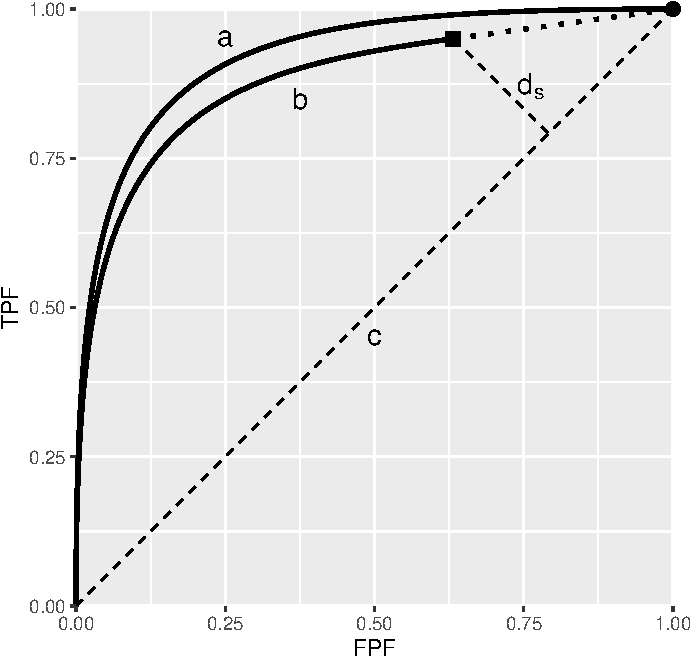
\includegraphics{10-rsm-search-classification_files/figure-latex/rsm-search-classification-performance-from-roc-curve-1.pdf}
\caption{\label{fig:rsm-search-classification-performance-from-roc-curve}Relation of lesion-localization performance to the end-point of the ROC curve. Plot (a) is using the binormal model while plot (b) is using a RSM predicted curve. The chance diagonal is labeled c.~The filled square is the end-point of the RSM predicted curve while the filled dot is the end-point of the binormal predicted curve. The distance of the filled square from the chance diagonal, labeled \(d_S\), is a measure of lesion-localization performance.}
\end{figure}

\emph{The location of the end-point, in particular how far it is from (1,1), is a measure of lesion-localization performance.} Higher lesion-localization performance is characterized by the end-point moving upwards and to the left, in the limit to (0,1), corresponding to perfect lesion-localization performance. It is more convenient to use a distance measure as defined next:

\textbf{Definition}

\begin{quote}
The perpendicular distance, \(d_S\), from the end-point to the chance diagonal, plot (c), multiplied by \(\sqrt{2}\), is the quantitative measure of lesion-localization performance denoted by \(L_L\).
\end{quote}

Using \href{https://en.wikipedia.org/wiki/Distance_from_a_point_to_a_line\#Line_defined_by_an_equation}{geometry} and Eqn. \eqref{eq:rsm-search-classification-FPF-TPF-max}, it follows that:

\begin{equation} 
L_L=\sqrt{2}d_S=\text{TPF}_{\text{max}}-\text{FPF}_{\text{max}}
\label{eq:rsm-search-classification-perp-distance}
\end{equation}

Therefore, lesion-localization performance \(L_L\) is given by:

\begin{equation} 
L_L=\exp\left ( -\lambda \right )\left (1-\sum_{L=1}^{L_{max}}f_L\left ( 1-\nu  \right )^L  \right )
\label{eq:rsm-search-classification-search-performance}
\end{equation}

Eqn. \eqref{eq:rsm-search-classification-search-performance} shows lesion-localization performance is the product of two terms: the probability \(\left (1-\sum_{L=1}^{L_{max}}f_L\left ( 1-\nu \right )^L \right )\) of finding at least one lesion times the probability \(\exp\left ( -\lambda \right )\) of not finding non-lesions. This puts into mathematical form the qualitative definition of lesion-localization performance as the ability to find lesions while avoiding finding non-lesions.

Example: consider \(\lambda = 0\) and \(\nu = 1\). (In terms of intrinsic parameters this occurs when \(\mu = \infty\).) The end-point is (0,1). The perpendicular distance from (0,1) to the chance diagonal is \(\frac{1}{\sqrt{2}}\), which multiplied by \(\sqrt{2}\) yields \(L_L = 1\). The same value is obtained using Eqn. \eqref{eq:rsm-search-classification-search-performance}. Since no NLs are found and all lesions are found, the observer never makes a mistake. One cannot improve over perfect performance and the observer does not need to use the z-sample information: he simply marks all suspicious regions found by the search mechanism regardless of their z-samples.

Search performance ranges from zero to one: \(0 \le L_L \le 1\). The lower limit is reached if \(\lambda = \infty\) or \(\nu = 0\). (In terms of intrinsic parameters this occurs when \(\mu = 0\).)

\hypertarget{rsm-search-classification-performance}{%
\section{Quantifying lesion-classification performance}\label{rsm-search-classification-performance}}

Lesion-classification performance \(L_C\) measures the ability, having found a suspicious region, to correctly classify it as a lesion, i.e., mark the location of the lesion resulting in a LL event. It is distinct from \emph{case-classification} performance, ROC AUC, which measures the ability to distinguish between diseased and non-diseased cases. In contrast \emph{lesion-classification} performance is a measure of the ability to distinguish between diseased and non-diseased regions, i.e., between latent NLs and latent LLs. \(L_C\) is determined by the \(\mu\) parameter of the RSM.

\textbf{Definition}

\begin{quote}
\(L_C\) is defined by the implied ROC-area of two unit variance normal distributions separated by \(\mu\) (see \href{https://dpc10ster.github.io/RJafrocRocBook/binormal-model.html\#binormal-model-d-prime}{formula} for d' measure in RJafrocRocBook).
\end{quote}

\begin{equation}
L_C=\Phi\left ( \frac{\mu}{\sqrt{2}} \right )
\label{eq:rsm-search-classification-classification-performance}
\end{equation}

Since \(\mu \ge 0\) it follows that \(L_C\) ranges from 0.5 to 1: \(0.5 \le L_C \le 1\). The lower limit occurs when \(\mu = 0\) and the upper limit occurs when \(\mu = \infty\).

\hypertarget{rsm-search-classification-discussion}{%
\section{Discussion}\label{rsm-search-classification-discussion}}

We have shown that the RSM parameters determine lesion-localization and lesion-classification performances. In the next chapter it will be shown that these parameters can be estimated from ROC/FROC data. Therefore the results of this chapter should be of interest to researchers in the area of computer aided detection -- CAD -- algorithm design, because they yield information about which stage -- lesion-localization or lesion-classification -- is limiting performance. If lesion-localization performance is low then the observer is having difficulty finding lesions while minimizing finding non-lesions \footnote{We repeat that a non-expert can trivally ``find'' all lesions by marking all regions in the image.}. In the CAD context, the \emph{initial detection} stage needs to be further optimized. If lesion-classification performance is low the observer is finding lesions efficiently but is having difficulty correctly classifying the found lesions. In the CAD context, the \emph{candidate analysis} stage needs to be further optimized. Of course, for this to be realized one needs a method for estimating the RSM parameters. This is the subject of the next chapter.

\hypertarget{part-cad-applications}{%
\part*{CAD applications}\label{part-cad-applications}}
\addcontentsline{toc}{part}{CAD applications}

\hypertarget{standalone-cad-radiologists}{%
\chapter{Standalone CAD}\label{standalone-cad-radiologists}}

\hypertarget{standalone-cad-radiologists-how-much-finished}{%
\section{How much finished}\label{standalone-cad-radiologists-how-much-finished}}

99\%

\hypertarget{standalone-cad-radiologists-introduction}{%
\section{Introduction}\label{standalone-cad-radiologists-introduction}}

In the US the majority of screening mammograms are analyzed by computer aided detection (CAD) algorithms \citep{rao2010widely}. Almost all major imaging device manufacturers provide CAD as part of their imaging workstation display software. In the United States CAD is approved for use as a second reader, i.e., the radiologist first interprets the images (typically 4 views, 2 views of each breast) without CAD and then CAD information (i.e., cued suspicious regions, possibly shown with associated probabilities of malignancies) is shown and the radiologist has the opportunity to revise the initial interpretation. In response to the FDA-approved second reader usage, the evolution of CAD algorithms has been guided mainly by comparing observer performance of radiologists with and without CAD.

Clinical CAD systems sometimes only report the locations of suspicious regions, i.e., it may not provide ratings. Analysis of this type of date is deferred to a following \textbf{TBA} chapter. However, a malignancy index (a continuous variable) for every CAD-found suspicious region is available to the algorithm designer \citep{edwards2002maximum}. Standalone performance, i.e., performance of designer-level CAD by itself, regarded as an algorithmic reader, vs.~radiologists, is rarely measured. In breast cancer screening I am aware of only one study \citep{hupse2013standalone} where standalone performance was measured. {[}Standalone performance has been measured in CAD for computed tomography colonography, chest radiography and three dimensional ultrasound \citep{hein2010computeraided, summers2008performance, taylor2006computerassisted, deBoo2011computeraided, tan2012computeraided}{]}.

One possible reason for not measuring standalone performance of CAD is the lack of an accepted assessment method for such measurements. This chapter removes that impediment. It describes a method for comparing standalone performance of designer-level CAD to a group of radiologists interpreting the same cases and compares the method to those described in two relevant publications \citep{hupse2013standalone, kooi2016comparison}.

\hypertarget{standalone-cad-radiologists-overview}{%
\section{Overview}\label{standalone-cad-radiologists-overview}}

This chapter extends the method used in a study of standalone CAD performance \citep{hupse2013standalone}, termed one-treatment random-reader fixed case or \textbf{1T-RRFC} analysis, since CAD is treated as an additional reader within a single treatment and since it only accounts for reader variability but does not account for case-variability.

The extension includes the effect of case-sampling variability and is hence termed one-treatment random-reader random-case or \textbf{1T-RRRC} analysis. The method is based on an existing method allowing comparison of the average performance of readers in a single treatment to a specified value. The key modification is to regard the difference in performance between radiologists over CAD as a figure of merit to which the existing work is directly applicable. The 1T-RRRC method is compared to 1T-RRFC.

The 1T-RRRC method is also compared to an unorthodox usage of conventional multiple-treatment multiple-reader method, termed \textbf{2T-RRRC} analysis, which involves replicating the CAD ratings as many times as there are radiologists, in effect simulating a second treatment, i.e., CAD is regarded as the second treatment (with identical readers within this treatment) to which existing methods (DBM or OR, as described in \href{https://dpc10ster.github.io/RJafrocRocBook/dbm-analysis-significance-testing.html}{RJafrocRocBook}) is applied.
`

\hypertarget{standalone-cad-radiologists-methods}{%
\section{Methods}\label{standalone-cad-radiologists-methods}}

Summarized are two relevant studies of CAD vs.~radiologists in mammography. This is followed by comments on the methods used in the two studies. The second study used multi-treatment multi-reader receiver operating characteristic (ROC) software in an unorthodox way. A statistical model and analysis method is described that avoids the unorthodox usage of ROC software and has fewer model parameters.

\hypertarget{standalone-cad-radiologists-two-previous-studies}{%
\subsection{Studies assessing performance of CAD vs.~radiologists}\label{standalone-cad-radiologists-two-previous-studies}}

The first study \citep{hupse2013standalone} measured performance in finding and localizing lesions in mammograms, i.e., visual search was involved, while the second study \citep{kooi2016comparison} measured lesion classification performance between non-diseased and diseased regions of interest (ROIs) previously found on mammograms by an independent algorithmic reader, i.e., visual search was not involved.

\hypertarget{standalone-cad-radiologists-study1}{%
\subsubsection{Study - 1}\label{standalone-cad-radiologists-study1}}

The first study \citep{hupse2013standalone} compared standalone performance of a CAD device to that of 9 radiologists interpreting the same cases (120 non-diseased and 80 with a single malignant mass per case). It used the LROC (localization ROC) paradigm \citep{starr1975visual, metz1976observer, swensson1996unified}, in which the observer gives an overall rating for presence of disease (an integer 0 to 100 scale was used) and indicates the location of the most suspicious region. On a non-diseased case the rating is classified as a false positive (FP) but on a diseased case it is classified as a \emph{correct localization} (CL) if the location is sufficiently close to the lesion and otherwise it is classified as an \emph{incorrect localization}. For a given reporting threshold, the number of correct localizations divided by the number of diseased cases estimates the probability of correct localization (PCL) at that threshold. On non-diseased cases the number of false positives (FPs) divided by the number of non-diseased cases estimates the probability of a false positive, or false positive fraction (FPF), at that threshold. The plot of PCL (ordinate) vs.~FPF defines the empirical LROC curve. Study - 1 used as figures of merit (FOMs) the interpolated PCL at two values of FPF, specifically FPF = 0.05 and FPF = 0.2, denoted \(\text{PCL}_{0.05}\) and \(\text{PCL}_{0.2}\), respectively. A t-test between the radiologist \(\text{PCL}_{\text{FPF}}\) values and that of CAD was used to compute the two-sided p-value for rejecting the NH of equal performance. Study - 1 reported p-value = 0.17 for \(\text{PCL}_{0.05}\) and p-value \(\leq\) 0.001, with CAD being inferior, for \(\text{PCL}_{0.2}\).

\hypertarget{standalone-cad-radiologists-study2}{%
\subsubsection{Study - 2}\label{standalone-cad-radiologists-study2}}

The second study \citep{kooi2016comparison} used 199 diseased and 199 non-diseased ROIs extracted by an independent CAD algorithm. These were analyzed by a different CAD algorithmic observer from that used to determine the ROIs and by four expert radiologists. In either case the ROC paradigm was used (i.e., a rating was obtained for each ROI) The figure of merit was the empirical area (AUC) under the respective ROC curves (one for each radiologist and one for CAD). The p-value for the difference in AUCs between the average radiologist's AUC and CAD AUC was determined using an unorthodox application of the Dorfman-Berbaum-Metz \citep{dorfman1992receiver} multiple-treatment multiple-reader multiple-case (DBM-MRMC) software.

The application was unorthodox in the sense that in the input data file \textbf{radiologists and CAD were entered as two treatments}. In conventional (or orthodox) DBM-MRMC each reader provides two ratings per case and the data file would consist of paired ratings of a set of cases interpreted by 4 readers. To accommodate the paired data structure assumed by the software, the authors of Study - 2 \textbf{replicated the CAD ratings four times in the input data file}, as explained in the caption to Table \ref{tab:standalone-cad-table-conventional}. By this artifice they converted a single-treatment 5-reader (4 radiologists plus CAD) data file to a two-treatment 4-reader data file in which the four readers in treatment 1 were the radiologists, and the four ``readers'' in treatment 2 were CAD replicated ratings. Note that for each case the four readers in the second treatment had identical ratings. In Table 1 the replicated CAD readers are labeled C1, C2, C3 and C4.

\begin{table}

\caption{\label{tab:standalone-cad-table-conventional}The differences between the data structures in conventional DBM-MRMC analysis and the unorthodox application of the software used in Study - 2. There are four radiologists, labeled R1, R2, R3 and R4 interpreting 398 cases labeled 1, 2, …, 398, in two treatments, labeled 1 and 2. Sample ratings are shown only for the first and last radiologist and the first and last case. In the first four columns, labeled "Standard DBM-MRMC", each radiologist interprets each case twice. In the next four columns, labeled "Unorthodox DBM-MRMC", the radiologists interpret each case once. CAD ratings are replicated four times to effectively create the second "treatment". The quotations emphasize that there is, in fact, only one treatment. The replicated CAD observers are labeled C1, C2, C3 and C4.}
\centering
\begin{tabular}[t]{lllllllll}
\toprule
\multicolumn{4}{c}{Standard DBM-MRMC} & \multicolumn{1}{c}{} & \multicolumn{4}{c}{Unorthodox DBM-MRMC} \\
\cmidrule(l{3pt}r{3pt}){1-4} \cmidrule(l{3pt}r{3pt}){6-9}
Reader & Treatment & Case & Rating &  & Reader & Treatment & Case & Rating\\
\midrule
R1 & 1 & 1 & 75 &  & R1 & 1 & 1 & 75\\
... & ... & ... & ... &  & ... & ... & ... & ...\\
R1 & 1 & 398 & 0 &  & R1 & 1 & 398 & 0\\
... & ... & ... & ... &  & ... & ... & ... & ...\\
R4 & 1 & 1 & 50 &  & R4 & 1 & 1 & 50\\
\addlinespace
... & ... & ... & ... &  & ... & ... & ... & ...\\
R4 & 1 & 398 & 25 &  & R4 & 1 & 398 & 25\\
 &  &  &  &  &  &  &  & \\
R1 & 2 & 1 & 45 &  & C1 & 2 & 1 & 55\\
... & ... & ... & ... &  & ... & ... & ... & ...\\
\addlinespace
R1 & 2 & 398 & 25 &  & C1 & 2 & 398 & 5\\
... & ... & ... & ... &  & ... & ... & ... & ...\\
R4 & 2 & 1 & 95 &  & C4 & 2 & 1 & 55\\
... & ... & ... & ... &  & ... & ... & ... & ...\\
R4 & 2 & 398 & 20 &  & C4 & 2 & 398 & 5\\
\bottomrule
\end{tabular}
\end{table}

Study -- 2 reported a not significant difference between CAD and the radiologists (p = 0.253).

\hypertarget{standalone-cad-radiologists-comments}{%
\subsubsection{Comments}\label{standalone-cad-radiologists-comments}}

For the purpose of this work, which focuses on the respective analysis methods, the difference in observer performance paradigms between the two studies, namely a search paradigm in Study - 1 vs.~an ROI classification paradigm in Study -- 2, is inconsequential. The paired t-test used in Study - 1 treats the case-sample as fixed. In other words, the analysis is not accounting for case-sampling variability but it is accounting for reader variability. While not explicitly stated, the reason for the unorthodox analysis in Study -- 2 was the desire to include case-sampling variability. Prof.~Karssemeijer (private communication, 10/27/2017) had consulted with a few ROC experts to determine if the procedure used in Study -- 2 was valid, and while the experts thought it was probably valid they were not sure.

In what follows, the analysis in Study -- 1 is referred to as \textbf{single-treatment random-reader fixed-case (1T-RRFC)} while that in Study -- 2 is referred to as \textbf{dual-treatment random-reader random-case (2T-RRRC)}.

\hypertarget{the-1t-rrfc-analysis-model}{%
\subsection{The 1T-RRFC analysis model}\label{the-1t-rrfc-analysis-model}}

The sampling model for the FOM is:

\begin{equation}
\left.
\begin{aligned}
\theta_j=\mu+R_j \\
\left (j = 1,2,...J  \right )
\end{aligned}
\right \}
\label{eq:standalone-1t-rrfc}
\end{equation}

Here \(\mu\) is a constant, \(\theta_j\) is the FOM for reader \(j\), and \(R_j\) is the random contribution for reader \(j\) distributed as:

\begin{equation}
R_j \sim  N\left ( 0,\sigma_R^2 \right )
\label{eq:standalone-cad-2t-rrfc-rj-sampling}
\end{equation}

Because of the assumed normal distribution of \(R_j\), in order to compare the readers to a fixed value, that of CAD denoted \(\theta_0\), one uses the (unpaired) t-test, as done in Study -- 1. As evident from the model, no allowance is made for case-sampling variability, which is the reason for calling it the 1T-RRFC method.

Performance of CAD on a fixed dataset does exhibit within-CAD variability, i.e., CAD applied repeatedly to a fixed dataset does not always produce the same mark-rating data. However, this source of within-CAD variability is much smaller than \emph{inter-reader} variability of radiologists interpreting the same dataset. The \emph{within-reader} variability of radiologists is smaller than \emph{inter-reader} variability and \emph{within-CAD} variability is even smaller. For this reason one is justified in regarded \(\theta_0\) as a fixed quantity for a given dataset. Varying the dataset will result in different values for \(\theta_0\) reflecting case sampling variability which needs to be accounted for as done in the following analyses.

\hypertarget{standalone-cad-radiologists-2TRRRC-anlaysis}{%
\subsection{The 2T-RRRC analysis model}\label{standalone-cad-radiologists-2TRRRC-anlaysis}}

This could be termed the conventional or the orthodox method. There are two treatments and the study design is fully crossed: each reader interprets each case in each treatment, i.e., the data structure is as in the left half of Table \ref{tab:standalone-cad-table-conventional}.

The following approach, termed 2T-RRRC, uses the Obuchowski and Rockette (OR) figure of merit sampling model \citep{obuchowski1995hypothesis}. The OR model is:

\begin{equation}
\theta_{ij\{c\}}=\mu+\tau_i+\left ( \tau \text{R} \right )_{ij}+\epsilon_{ij\{c\}}
\label{eq:standalone-cad-model-2t-rrrc}
\end{equation}

Assuming two treatments, \(i\) (\(i = 1, 2\)) is the treatment index, \(j\) (\(j = 1, ..., J\)) is the reader index, and \(k\) (\(k = 1, ..., K\)) is the case index, and \(\theta_{ij\{c\}}\) is the figure of merit in treatment \(i\) for reader \(j\) and case-sample \(\{c\}\). A case-sample is a set or ensemble of cases, diseased and non-diseased, and different integer values of \(c\) correspond to different case-samples.

The first two terms on the right hand side of Eqn. \eqref{eq:standalone-cad-model-2t-rrrc} are fixed effects (average performance and treatment effect, respectively). The next two terms are random effect variables that, by assumption, are sampled as follows:

\begin{equation}
\left.
\begin{aligned}  
R_j \sim  N\left ( 0,\sigma_R^2 \right )\\
\left ( \tau R \right )_{ij} \sim N\left ( 0,\sigma_{\tau R}^2 \right )\\
\end{aligned}
\right \}
\label{eq:standalone-cad-2t-r-taur-sampling}
\end{equation}

The terms \(R_j\) represents the random treatment-independent contribution of reader \(j\), modeled as a sample from a zero-mean normal distribution with variance \(\sigma_R^2\), \(\left ( \tau R \right )_{ij}\) represents the random treatment-dependent contribution of reader \(j\) in treatment \(i\), modeled as a sample from a zero-mean normal distribution with variance \(\sigma_{\tau R}^2\). The sampling of the last (error) term is described by:

\begin{equation}
\epsilon_{ij\{c\}}\sim N_{I \times J}\left ( \vec{0} , \Sigma \right )
\label{eq:standalone-cad-2t-eps-sampling}
\end{equation}

Here \(N_{I \times J}\) is the \(I \times J\) variate normal distribution and \(\vec{0}\), a \(I \times J\) length zero-vector, represents the mean of the distribution. The \(\{I \times J\} \times \{I \times J\}\) dimensional covariance matrix \(\Sigma\) is defined by 4 parameters, \(\text{Var}\), \(\text{Cov}_1\), \(\text{Cov}_2\), \(\text{Cov}_3\), defined as follows:

\begin{equation}
\text{Cov} \left (\epsilon_{ij\{c\}},\epsilon_{i'j'\{c\}} \right ) =
\left\{\begin{matrix}
\text{Var} \; (i=i',j=j') \\
\text{Cov1} \; (i\ne i',j=j')\\ 
\text{Cov2} \; (i = i',j \ne j')\\ 
\text{Cov3} \; (i\ne i',j \ne j')
\end{matrix}\right\}
\label{eq:standalone-cad-2t-rrrc-cov}
\end{equation}

Software \{U of Iowa and \texttt{RJafroc}\} yields estimates of all terms appearing on the right hand side of Eqn. \eqref{eq:standalone-cad-2t-rrrc-cov}. Excluding fixed effects the model represented by Eqn. \eqref{eq:standalone-cad-model-2t-rrrc} contains six parameters:

\begin{equation}
\sigma_R^2, \sigma_{\tau R}^2, \text{Var}, \text{Cov}_1, \text{Cov}_2, \text{Cov}_3
\label{eq:standalone-cad-2t-rrrc-varcom}
\end{equation}

The meanings the last four terms are described in \citep{hillis2007comparison, obuchowski1995hypothesis, hillis2005comparison, chakraborty2017observer}. Briefly, \(\text{Var}\) is the variance of a reader's FOMs, in a given treatment, over interpretations of different case-samples, averaged over readers and treatments; \(\text{Cov}_1/\text{Var}\) is the correlation of a reader's FOMs, over interpretations of different case-samples in different treatments, averaged over all different-treatment same-reader pairings; \(\text{Cov}_2/\text{Var}\) is the correlation of different reader's FOMs, over interpretations of different case-samples in the same treatment, averaged over all same- treatment different-reader pairings and finally, \(\text{Cov}_3/\text{Var}\) is the correlation of different reader's FOMs, over interpretations of different case-samples in different treatments, averaged over all different-treatment different-reader pairings. One expects the following inequalities to hold:

\begin{equation}
\text{Var} \geq \text{Cov}_1 \geq \text{Cov}_2 \geq \text{Cov}_3
\label{eq:standalone-cad-2t-rrrc-varcom-ordering}
\end{equation}

In practice, since one is usually limited to one case-sample, i.e., \(c = 1\), resampling techniques \citep{efron1994introduction} -- e.g., the jackknife -- are used to estimate these terms.

\hypertarget{standalone-cad-radiologists-1TRRRC-anlaysis}{%
\subsection{The 1T-RRRC analysis model}\label{standalone-cad-radiologists-1TRRRC-anlaysis}}

The difference from the approach in Study - 2, and the main contribution of this work, is to regard standalone CAD as a different reader, not as a different treatment. This section describes a single treatment method for analyzing readers and CAD, where CAD is regarded as an additional reader and artificially replicated CAD data becomes unnecessary. Accordingly the proposed method is termed \textbf{single-treatment random-reader random-case (1T-RRRC)} analysis.

The starting point is the \citep{obuchowski1995hypothesis} model for a single treatment, which for the radiologists (i.e., \emph{excluding} CAD) interpreting in a single-treatment reduces to the following model:

\begin{equation}
\theta_{j\{c\}}=\mu+R_j+\epsilon_{j\{c\}}
\label{eq:standalone-or-model-single-treatment}
\end{equation}

\(\theta_{j\{c\}}\) is the figure of merit for radiologist \(j\) (\(j = 1, 2, ..., J\)) interpreting case-sample \(\{c\}\); \(R_j\) is the random effect of radiologist \(j\) and \(\epsilon_{j\{c\}}\) is the error term. For single-treatment multiple-reader interpretations the error term is distributed as:

\begin{equation}
\epsilon_{j\{c\}}\sim N_{J}\left ( \vec{0} , \Sigma \right )
\label{eq:standalone-cad-1t-eps-sampling}
\end{equation}

The \(J \times J\) covariance matrix \(\Sigma\) is defined by two parameters, \(\text{Var}\) and \(\text{Cov}_2\), as follows:

\begin{equation}
\Sigma_{jj'} = \text{Cov}\left ( \epsilon_{j\{c\}}, \epsilon_{j'\{c\}} \right )
=
\left\{\begin{matrix}
\text{Var} & j = j'\\ 
\text{Cov}_2 & j \neq j'
\end{matrix}\right.
\label{eq:standalone-cad-1t-var-cov2-sampling}
\end{equation}

In practice the terms \(\text{Var}\) and \(\text{Cov}_2\) are estimated using the jackknife method.

\hypertarget{single-treatment-analysis-for-radiologists}{%
\subsubsection{Single treatment analysis for radiologists}\label{single-treatment-analysis-for-radiologists}}

Hillis \citep{hillis2005comparison, hillis2007comparison} has described how to use the single treatment model \eqref{eq:standalone-or-model-single-treatment} to compare a groups of radiologists' average performance to a fixed value, in effect the \(\text{NH}: \mu = \mu_0\), where \(\mu_0\) is a pre-specified constant.

One might be tempted to set \(\mu_0\) equal to the performance of CAD but that would not be accounting for the fact that the performance of CAD is itself a random variable whose case-sampling variability needs to be accounted for.

\hypertarget{adaptation-of-single-treatment-analysis-to-accommodate-cad}{%
\subsubsection{Adaptation of single treatment analysis to accommodate CAD}\label{adaptation-of-single-treatment-analysis-to-accommodate-cad}}

Instead, the following model is used for the figure of merit of the radiologists \textbf{and} CAD (note that \(j = 0\) is used to denote the CAD algorithmic reader):

\begin{equation}
\theta_{j\{c\}} = \theta_{0\{c\}} + \Delta \theta + R_j + \epsilon_{j\{c\}}\\
j=1,2,...J
\label{eq:standalone-cad-1t-thetaj}
\end{equation}

\(\theta_{0\{c\}}\) is the CAD figure of merit for case-sample \(\{c\}\) and \(\Delta \theta\) is the average figure of merit increment of the radiologists over CAD. To reduce this model to one to which Hillis' formulae are directly applicable, one subtracts the CAD figure of merit from each radiologist's figure of merit for the same case-sample, and defines this as the difference figure of merit \(\psi_{j\{c\}}\) , i.e.,

\begin{equation}
\psi_{j\{c\}} = \theta_{j\{c\}} - \theta_{0\{c\}}
\label{eq:standalone-cad-diff-reader-def}
\end{equation}

Then Eqn. \eqref{eq:standalone-cad-1t-thetaj} reduces to:

\begin{equation}
\psi_{j\{c\}} = \Delta \theta + R_j + \epsilon_{j\{c\}}
\label{eq:standalone-cad-1t-psi}
\end{equation}

Eqn. \eqref{eq:standalone-cad-1t-psi} is identical in form to Eqn. \eqref{eq:standalone-or-model-single-treatment} excepting that the figure of merit on the left hand side of Eqn. \eqref{eq:standalone-cad-1t-psi} is a \emph{difference FOM}, that between the radiologist's and CAD, i.e., describing a model for \(J\) radiologists interpreting a common case set, each of whose performances is measured \emph{relative} to that of CAD. Under the NH the expected difference is zero: \(\text{NH:} \Delta \theta = 0\). The method \citep{hillis2005comparison, hillis2007comparison} for single-treatment multiple-reader analysis is now directly applicable to the model described by Eqn. \eqref{eq:standalone-cad-1t-psi}.

Apart from fixed effects, the model in Eqn. \eqref{eq:standalone-cad-1t-psi} contains three parameters:

\begin{equation}
\sigma_R^2, \text{Var}, \text{Cov}_2
\label{eq:standalone-cad-1t-parms}
\end{equation}

Setting \(\text{Var} = 0, \text{Cov}_2 = 0\) yields the 1T-RRFC model which contains only one random parameter, namely \(\sigma_R^2\). One expects an identical estimate of this parameter using 1T-RRRC analyses.

\hypertarget{standalone-cad-radiologists-computational-details}{%
\section{Implementation}\label{standalone-cad-radiologists-computational-details}}

The three analyses, namely random-reader fixed-case (1T-RRFC), dual-treatment random-reader random-case (2T-RRRC) and single-treatment random-reader random-case (1T-RRRC), are implemented in \texttt{RJafroc}.

The following code shows usage of the software to generate the results. Note that \texttt{RJafroc::datasetCadLroc} is the LROC dataset and \texttt{RJafroc::dataset09} is the corresponding ROC dataset.

\begin{Shaded}
\begin{Highlighting}[]
\NormalTok{RRFC\_1T\_PCL\_0\_05 }\OtherTok{\textless{}{-}}\NormalTok{ RJafroc}\SpecialCharTok{::}\FunctionTok{StSignificanceTestingCadVsRad}\NormalTok{ (RJafroc}\SpecialCharTok{::}\NormalTok{datasetCadLroc, }
\AttributeTok{FOM =} \StringTok{"PCL"}\NormalTok{, }\AttributeTok{FPFValue =} \FloatTok{0.05}\NormalTok{, }\AttributeTok{method =} \StringTok{"1T{-}RRFC"}\NormalTok{)}
\NormalTok{RRRC\_2T\_PCL\_0\_05 }\OtherTok{\textless{}{-}}\NormalTok{ RJafroc}\SpecialCharTok{::}\FunctionTok{StSignificanceTestingCadVsRad}\NormalTok{ (RJafroc}\SpecialCharTok{::}\NormalTok{datasetCadLroc, }
\AttributeTok{FOM =} \StringTok{"PCL"}\NormalTok{, }\AttributeTok{FPFValue =} \FloatTok{0.05}\NormalTok{, }\AttributeTok{method =} \StringTok{"2T{-}RRRC"}\NormalTok{)}
\NormalTok{RRRC\_1T\_PCL\_0\_05 }\OtherTok{\textless{}{-}}\NormalTok{ RJafroc}\SpecialCharTok{::}\FunctionTok{StSignificanceTestingCadVsRad}\NormalTok{ (RJafroc}\SpecialCharTok{::}\NormalTok{datasetCadLroc, }
\AttributeTok{FOM =} \StringTok{"PCL"}\NormalTok{, }\AttributeTok{FPFValue =} \FloatTok{0.05}\NormalTok{, }\AttributeTok{method =} \StringTok{"1T{-}RRRC"}\NormalTok{)}

\NormalTok{RRFC\_1T\_PCL\_0\_2 }\OtherTok{\textless{}{-}}\NormalTok{ RJafroc}\SpecialCharTok{::}\FunctionTok{StSignificanceTestingCadVsRad}\NormalTok{ (RJafroc}\SpecialCharTok{::}\NormalTok{datasetCadLroc, }
\AttributeTok{FOM =} \StringTok{"PCL"}\NormalTok{, }\AttributeTok{FPFValue =} \FloatTok{0.2}\NormalTok{, }\AttributeTok{method =} \StringTok{"1T{-}RRFC"}\NormalTok{)}
\NormalTok{RRRC\_2T\_PCL\_0\_2 }\OtherTok{\textless{}{-}}\NormalTok{ RJafroc}\SpecialCharTok{::}\FunctionTok{StSignificanceTestingCadVsRad}\NormalTok{ (RJafroc}\SpecialCharTok{::}\NormalTok{datasetCadLroc, }
\AttributeTok{FOM =} \StringTok{"PCL"}\NormalTok{, }\AttributeTok{FPFValue =} \FloatTok{0.2}\NormalTok{, }\AttributeTok{method =} \StringTok{"2T{-}RRRC"}\NormalTok{)}
\NormalTok{RRRC\_1T\_PCL\_0\_2 }\OtherTok{\textless{}{-}}\NormalTok{ RJafroc}\SpecialCharTok{::}\FunctionTok{StSignificanceTestingCadVsRad}\NormalTok{ (RJafroc}\SpecialCharTok{::}\NormalTok{datasetCadLroc, }
\AttributeTok{FOM =} \StringTok{"PCL"}\NormalTok{, }\AttributeTok{FPFValue =} \FloatTok{0.2}\NormalTok{, }\AttributeTok{method =} \StringTok{"1T{-}RRRC"}\NormalTok{)}

\NormalTok{RRFC\_1T\_PCL\_1 }\OtherTok{\textless{}{-}}\NormalTok{ RJafroc}\SpecialCharTok{::}\FunctionTok{StSignificanceTestingCadVsRad}\NormalTok{ (RJafroc}\SpecialCharTok{::}\NormalTok{datasetCadLroc, }
\AttributeTok{FOM =} \StringTok{"PCL"}\NormalTok{, }\AttributeTok{FPFValue =} \DecValTok{1}\NormalTok{, }\AttributeTok{method =} \StringTok{"1T{-}RRFC"}\NormalTok{)}
\NormalTok{RRRC\_2T\_PCL\_1 }\OtherTok{\textless{}{-}}\NormalTok{ RJafroc}\SpecialCharTok{::}\FunctionTok{StSignificanceTestingCadVsRad}\NormalTok{ (RJafroc}\SpecialCharTok{::}\NormalTok{datasetCadLroc, }
\AttributeTok{FOM =} \StringTok{"PCL"}\NormalTok{, }\AttributeTok{FPFValue =} \DecValTok{1}\NormalTok{, }\AttributeTok{method =} \StringTok{"2T{-}RRRC"}\NormalTok{)}
\NormalTok{RRRC\_1T\_PCL\_1 }\OtherTok{\textless{}{-}}\NormalTok{ RJafroc}\SpecialCharTok{::}\FunctionTok{StSignificanceTestingCadVsRad}\NormalTok{ (RJafroc}\SpecialCharTok{::}\NormalTok{datasetCadLroc, }
\AttributeTok{FOM =} \StringTok{"PCL"}\NormalTok{, }\AttributeTok{FPFValue =} \DecValTok{1}\NormalTok{, }\AttributeTok{method =} \StringTok{"1T{-}RRRC"}\NormalTok{)}

\NormalTok{RRFC\_1T\_AUC }\OtherTok{\textless{}{-}}\NormalTok{ RJafroc}\SpecialCharTok{::}\FunctionTok{StSignificanceTestingCadVsRad}\NormalTok{ (RJafroc}\SpecialCharTok{::}\NormalTok{dataset09, }
\AttributeTok{FOM =} \StringTok{"Wilcoxon"}\NormalTok{, }\AttributeTok{method =} \StringTok{"1T{-}RRFC"}\NormalTok{)}
\NormalTok{RRRC\_2T\_AUC }\OtherTok{\textless{}{-}}\NormalTok{ RJafroc}\SpecialCharTok{::}\FunctionTok{StSignificanceTestingCadVsRad}\NormalTok{ (RJafroc}\SpecialCharTok{::}\NormalTok{dataset09, }
\AttributeTok{FOM =} \StringTok{"Wilcoxon"}\NormalTok{, }\AttributeTok{method =} \StringTok{"2T{-}RRRC"}\NormalTok{)}
\NormalTok{RRRC\_1T\_AUC }\OtherTok{\textless{}{-}}\NormalTok{ RJafroc}\SpecialCharTok{::}\FunctionTok{StSignificanceTestingCadVsRad}\NormalTok{ (RJafroc}\SpecialCharTok{::}\NormalTok{dataset09, }
\AttributeTok{FOM =} \StringTok{"Wilcoxon"}\NormalTok{, }\AttributeTok{method =} \StringTok{"1T{-}RRRC"}\NormalTok{)}
\end{Highlighting}
\end{Shaded}

The results are organized as follows:

\begin{itemize}
\item
  \texttt{RRFC\_1T\_PCL\_0\_05} contains the results of 1T-RRFC analysis for figure of merit = \(\text{PCL}_{0.05}\).
\item
  \texttt{RRRC\_2T\_PCL\_0\_05} contains the results of 2T-RRRC analysis for figure of merit = \(\text{PCL}_{0.05}\).
\item
  \texttt{RRRC\_1T\_PCL\_0\_05} contains the results of 1T-RRRC analysis for figure of merit = \(\text{PCL}_{0.05}\).
\item
  \texttt{RRFC\_1T\_PCL\_0\_2} contains the results of 1T-RRFC analysis for figure of merit = \(\text{PCL}_{0.2}\).
\item
  \texttt{RRRC\_2T\_PCL\_0\_2} contains the results of 2T-RRRC analysis for figure of merit = \(\text{PCL}_{0.2}\).
\item
  \texttt{RRRC\_1T\_PCL\_0\_2} contains the results of 1T-RRRC analysis for figure of merit = \(\text{PCL}_{0.2}\).
\item
  \texttt{RRFC\_1T\_AUC} contains the results of 1T-RRFC analysis for the Wilcoxon figure of merit.
\item
  \texttt{RRRC\_2T\_AUC} contains the results of 2T-RRRC analysis for the Wilcoxon figure of merit.
\item
  \texttt{RRRC\_1T\_AUC} contains the results of 1T-RRRC analysis for the Wilcoxon figure of merit.
\end{itemize}

The structures of these objects are illustrated with examples in the Appendix.

\hypertarget{standalone-cad-radiologists-results}{%
\section{Results}\label{standalone-cad-radiologists-results}}

The three methods, 1T-RRFC, 2T-RRRC and 1T-RRRC, were applied to an LROC dataset similar to that used in Study -- 1 (I thank Prof.~Karssemeijer for making this dataset available), Table \ref{tab:standalone-cad-table2}.

\begin{table}

\caption{\label{tab:standalone-cad-table2}Significance testing results for an LROC dataset. For each figure of merit (FOM) shown are results of RRRC, 2T-RRRC and 1T-RRRC analyses. Because it is accounting for an additional source of variability, each of the rows labeled RRRC yields a larger p-value and wider confidence interval than the corresponding row labeled RRFC. [$\theta_0$ = FOM CAD; $\theta_{\bullet}$ = average FOM of radiologists; $\psi_{\bullet}$ = average FOM of radiologists minus CAD; CI= 95 percent confidence interval of quantity indicated by the subscript, F = F-statistic; ddf = denominator degrees of freedom; p = p-value for rejecting the null hypothesis: $\psi_{\bullet} = 0$.]}
\centering
\fontsize{10}{12}\selectfont
\begin{tabular}[t]{lllllllllll}
\toprule
FOM & Analysis & $\theta_0$ & $CI_{\theta_0}$ & $\theta_{\bullet}$ & $CI_{\theta_{\bullet}}$ & $\psi_{\bullet}$ & $CI_{\psi_{\bullet}}$ & F & ddf & p\\
\midrule
PCL\_0\_05 & 1T-RRFC & 0.45 & NA & 0.493 & (0.42,0.57) & 0.0433 & (-0.032,0.12) & 1.8 & 8 & 0.22\\
 & 2T-RRRC &  & (0.26,0.64) &  & (0.38,0.61) &  & (-0.16,0.24) & 0.18 & 784 & 0.67\\
 & 1T-RRRC &  & NA &  & (0.29,0.69) &  & (-0.16,0.24) & 0.18 & 784 & 0.67\\
PCL\_0\_2 & 1T-RRFC & 0.592 & NA & 0.71 & (0.67,0.75) & 0.119 & (0.078,0.16) & 45 & 8 & 0.00015\\
 & 2T-RRRC &  & (0.48,0.71) &  & (0.63,0.79) &  & (0.0044,0.23) & 4.2 & 937 & 0.042\\
\addlinespace
 & 1T-RRRC &  & NA &  & (0.6,0.82) &  & (0.0044,0.23) & 4.2 & 937 & 0.042\\
PCL\_1 & 1T-RRFC & 0.675 & NA & 0.783 & (0.74,0.83) & 0.108 & (0.065,0.15) & 33 & 8 & 0.00043\\
 & 2T-RRRC &  & (0.57,0.78) &  & (0.71,0.85) &  & (0.0045,0.21) & 4.2 & 493 & 0.041\\
 & 1T-RRRC &  & NA &  & (0.68,0.89) &  & (0.0045,0.21) & 4.2 & 493 & 0.041\\
Wilcoxon & 1T-RRFC & 0.817 & NA & 0.849 & (0.83,0.87) & 0.0317 & (0.009,0.055) & 10 & 8 & 0.012\\
\addlinespace
 & 2T-RRRC &  & (0.75,0.88) &  & (0.81,0.89) &  & (-0.031,0.094) & 0.99 & 878 & 0.32\\
 & 1T-RRRC &  & NA &  & (0.79,0.91) &  & (-0.031,0.094) & 0.99 & 878 & 0.32\\
\bottomrule
\end{tabular}
\end{table}

Results are shown for the following FOMs: \(\text{PCL}_{0.05}\), \(\text{PCL}_{0.2}\), \(\text{PCL}_{1}\) and the empirical area (AUC) under the ROC curve estimated by the Wilcoxon statistic. The first two FOMs are identical to those used in Study -- 1. Columns 3 and 4 list the CAD FOM \(\theta_0\) and its 95\% confidence interval \(CI_{\theta_0}\), columns 5 and 6 list the average radiologist FOM \(\theta_{\bullet}\) (the dot symbol represents an average over the non-zero radiologist index j = 1,2,\ldots, 9) and its 95\% confidence interval \(CI_{\theta_{\bullet}}\), columns 7 and 8 list the average difference FOM \(\psi_{\bullet}\), i.e., radiologist average minus CAD, and its 95\% confidence interval \(CI_{\psi_{\bullet}}\), and the last three columns list the F-statistic, the denominator degrees of freedom (ddf) and the p-value for rejecting the null hypothesis (the numerator degree of freedom of the F-statistic is unity).

\begin{quote}
\textbf{The last three columns show that 2T-RRRC and 1T-RRRC analyses yield identical F-statistics, ddf and p-values}. So the intuition of the authors of Study -- 2, that the unorthodox method of using DBM -- MRMC software to account for both reader and case-sampling variability, turns out to be correct. If interest is solely in these statistics one is justified in using the unorthodox method. Important caveats are noted below.
\end{quote}

Other results evident in Table \ref{tab:standalone-cad-table2}:

\begin{enumerate}
\def\labelenumi{\arabic{enumi}.}
\tightlist
\item
  Where a direct comparison is possible, namely 1T-RRFC analysis using \(\text{PCL}_{0.05}\) and \(\text{PCL}_{0.2}\) as FOMs, the p-values in Table \ref{tab:standalone-cad-table2} are very close to those reported in Study -- 1.
\item
  All FOMs (i.e., \(\theta_0\), \(\theta_{\bullet}\) and \(\psi_{\bullet}\)) in Table \ref{tab:standalone-cad-table2} are independent of the method of analysis. However, the corresponding confidence intervals (i.e., \(CI_{\theta_0}\), \(CI_{\theta_{\bullet}}\) and \(CI_{\psi_{\bullet}}\)) depend on the analyses.
\item
  Since the CAD figure of merit is a constant no confidence interval is appropriate for it for either 1T-RRFC or 1T-RRRC analysis and the listed values are NA (not applicable). Since 2T-RRRC analysis assumes CAD is a different treatment the analysis lists a confidence interval that is correctly centered on the CAD value but is otherwise meaningless, i.e., it is an artifact of the unintended usage of the OR analysis method.
\item
  The p-value for either RRRC analyses (2T or 1T) is larger than the corresponding 1T-RRFC value. Accounting for case-sampling variability increases the p-value leading to less possibility of finding a significant difference.
\item
  The LROC FOMs increase as the value of FPF (the subscript) increases, a general feature of any partial curve based figure of merit, as is the observation that the area (AUC) under the ROC is larger than the largest PCL value.
\item
  Using either RRRC analyses ignoring localization information (i.e., using the AUC FOM) leads to a not-significant difference between CAD and the radiologists (\(p\) = 0.32) while using localization information via the \(\text{PCL}_1\) FOM yields a significant difference (\(p\) = 0.041), consistent with the expectation that using localization information leads to increased statistical power.
\item
  Partial curve-based FOMs, such as \(\text{PCL}_\text{FPF}\), lead, depending on the choice of \(\text{FPF}\), to different conclusions on whether to reject the NH. Using either RRRC analyses the p-values decrease as \(\text{FPF}\) increases (e.g., \$ 0.67 \textgreater{} 0.042 \textgreater{} 0.041\$). This trend is not observed for 1T-RRFC analysis which shows a ``sweet-spot'' effect where the p-value has a minimum for \(\text{FPF} = 0.2\)
\end{enumerate}

Shown next, Table \ref{tab:standalone-cad-table3}, are the model-parameters corresponding to the three analyses.

\begin{table}

\caption{\label{tab:standalone-cad-table3}Significance testing results for an LROC dataset. For each figure of merit (FOM) shown are results of RRRC, 2T-RRRC and 1T-RRRC analyses. Because it is accounting for an additional source of variability, each of the rows labeled RRRC yields a larger p-value and wider confidence interval than the corresponding row labeled RRFC. [$\theta_0$ = FOM CAD; $\theta_{\bullet}$ = average FOM of radiologists; $\psi_{\bullet}$ = average FOM of radiologists minus CAD; CI= 95 percent confidence interval of quantity indicated by the subscript, F = F-statistic; ddf = denominator degrees of freedom; p = p-value for rejecting the null hypothesis: $\psi_{\bullet} = 0$.]}
\centering
\fontsize{10}{12}\selectfont
\begin{tabular}[t]{llllllll}
\toprule
FOM & Analysis & $\sigma_R^2$ & $\sigma_{\tau R}^2$ & Cov1 & Cov2 & Cov3 & Var\\
\midrule
PCL\_0\_05 & 1T-RRFC & 0.0095 & NA & NA & NA & NA & NA\\
 & 2T-RRRC & 1.8e-18 & -0.00571 & 0.00131 & 0.00601 & 0.00131 & 0.0165\\
 & 1T-RRRC & 0.0095 & NA & NA & 0.0094 & NA & 0.0303\\
PCL\_0\_2 & 1T-RRFC & 0.00281 & NA & NA & NA & NA & NA\\
 & 2T-RRRC & -7.6e-19 & 0.000265 & 0.000761 & 0.00229 & 0.000761 & 0.00343\\
\addlinespace
 & 1T-RRRC & 0.00281 & NA & NA & 0.00307 & NA & 0.00534\\
PCL\_1 & 1T-RRFC & 0.0032 & NA & NA & NA & NA & NA\\
 & 2T-RRRC & 1.6e-18 & 0.001 & 0.000643 & 0.00186 & 0.000643 & 0.00246\\
 & 1T-RRRC & 0.0032 & NA & NA & 0.00244 & NA & 0.00364\\
Wilcoxon & 1T-RRFC & 0.000878 & NA & NA & NA & NA & NA\\
\addlinespace
 & 2T-RRRC & 3e-19 & 0.000201 & 0.000262 & 0.000724 & 0.000262 & 0.000962\\
 & 1T-RRRC & 0.000878 & NA & NA & 0.000924 & NA & 0.0014\\
\bottomrule
\end{tabular}
\end{table}

From Table \ref{tab:standalone-cad-table3} some inconsistencies are evident for 2T-RRRC analysis:

\begin{enumerate}
\def\labelenumi{\arabic{enumi}.}
\tightlist
\item
  For 2T-RRRC analyses the listed values for \(\sigma_R^2\) are smaller than machine accuracy, therefore one concludes that in fact \(\sigma_R^2 = 0\) which is \textbf{clearly an incorrect result as the radiologists do not have identical performances}. In contrast, 1T-RRRC analyses yields the expected non-zero values, identical to those obtained by 1T-RRFC analyses (see comment following Eqn. \eqref{eq:standalone-cad-1t-parms}).
\item
  For the 2T\_RRRC method the expected ordering of the inequalities, Eqn. \eqref{eq:standalone-cad-2t-rrrc-varcom-ordering} is not observed: one expects \(\text{Cov}_1 \geq \text{Cov}_2 \geq \text{Cov}_3\) but instead one observes \(\text{Cov}_1 = \text{Cov}_3\) and \(\text{Cov}_2 > \text{Cov}_1\).
\end{enumerate}

The design of a ratings simulator to statistically match a given dataset is addressed in Chapter 23 of my print book \citep{chakraborty2017observer}. Using this simulator, the 1T-RRRC method had the expected null hypothesis behavior (Table 23.5, ibid).

\hypertarget{standalone-cad-radiologists-discussion}{%
\section{Discussion}\label{standalone-cad-radiologists-discussion}}

Described is an extension of the analysis used in Study -- 1 that accounts for case sampling variability. It extends \citep{hillis2005comparison} single-treatment analysis to a situation where one of the ``readers'' is a special reader subject to case-sampling variability only, and the desire is to compare performance of this special reader to the average of the remaining readers. Usage of the method along with two other methods is illustrated using an LROC dataset.

The proposed method, 1T-RRRC analyses, yields identical ``overall'' results (specifically the F-statistic, degrees of freedom and p-value) to those yielded by the unorthodox application of commonly available software, termed 2T-RRRC analyses, where the CAD reader is regarded as a second treatment (specifically the CAD ratings are replicated to match the number of radiologists). If interest is in just these values one is justified in using the 2T-RRRC method. However, 2T-RRRC model parameter estimates were unrealistic: for example, it yields zero between-reader variance. The result \(\sigma_R^2 = 0\) is clearly an artifact. One can only speculate as to what happens when software is used in a manner that it was not designed for: perhaps finding that all readers in the second treatment have identical FOMs led the software to yield \(\sigma_R^2 = 0\). Additionally, the covariance estimates are incorrect. Since sample-size estimation requires some of the covariance values the 2T-RRRC method should never be used to perform sample-size estimation for a prospective study.

The 1T-RRRC method described here is applicable to any scalar figure of merit. The paradigm used to collect the observer performance data - ROC, FROC, LROC or ROI - is irrelevant.

Assessing CAD utility by measuring performance with and without CAD may have inadvertently set a low bar for CAD to be considered useful. As examples, CAD is not penalized for missing cancers as long as the radiologist finds them and CAD is not penalized for excessive false positives (FPs) as long as the radiologist ignores them. Moreover, since both such measurements include the variability of radiologists, there is additional noise introduces that presumably makes it harder to determine if the CAD system is optimal.

In my opinion standalone performance is the most direct measure of CAD performance. Lack of a clear-cut method for assessing standalone CAD performance may have limited past CAD research. The current work hopefully removes that impediment. Going forward, assessment of standalone performance of CAD vs.~expert radiologists is strongly encouraged.

\hypertarget{standalone-cad-radiologists-appendix1}{%
\section{Appendix 1}\label{standalone-cad-radiologists-appendix1}}

The structures of the\texttt{R} objects generated by the software are illustrated with three examples.

\hypertarget{example-1}{%
\subsection{Example 1}\label{example-1}}

The first example shows the structure of \texttt{RRFC\_1T\_PCL\_0\_2}.

\begin{Shaded}
\begin{Highlighting}[]
\NormalTok{x }\OtherTok{\textless{}{-}}\NormalTok{ RRFC\_1T\_PCL\_0\_2}
\NormalTok{fom\_individual\_rad }\OtherTok{\textless{}{-}} \FunctionTok{as.data.frame}\NormalTok{(}\FunctionTok{t}\NormalTok{(x}\SpecialCharTok{$}\NormalTok{fomRAD))}
\FunctionTok{colnames}\NormalTok{(fom\_individual\_rad) }\OtherTok{\textless{}{-}} \FunctionTok{paste0}\NormalTok{(}\StringTok{"rdr"}\NormalTok{, }\FunctionTok{seq}\NormalTok{(}\DecValTok{1}\SpecialCharTok{:}\DecValTok{9}\NormalTok{))}

\NormalTok{stats }\OtherTok{\textless{}{-}} \FunctionTok{data.frame}\NormalTok{(}\AttributeTok{fomCAD =}\NormalTok{ x}\SpecialCharTok{$}\NormalTok{fomCAD, }\AttributeTok{avgRadFom =}\NormalTok{ x}\SpecialCharTok{$}\NormalTok{avgRadFom, }\AttributeTok{avgDiffFom =}\NormalTok{ x}\SpecialCharTok{$}\NormalTok{avgDiffFom, }\AttributeTok{varR =}\NormalTok{ x}\SpecialCharTok{$}\NormalTok{varR, }\AttributeTok{Tstat =}\NormalTok{ x}\SpecialCharTok{$}\NormalTok{Tstat, }\AttributeTok{df =}\NormalTok{ x}\SpecialCharTok{$}\NormalTok{df, }\AttributeTok{pval =}\NormalTok{ x}\SpecialCharTok{$}\NormalTok{pval)}

\NormalTok{ConfidenceIntervals }\OtherTok{\textless{}{-}} \FunctionTok{data.frame}\NormalTok{(}\AttributeTok{CIAvgRadFom =}\NormalTok{ x}\SpecialCharTok{$}\NormalTok{CIAvgRadFom, }\AttributeTok{CIAvgDiffFom =}\NormalTok{ x}\SpecialCharTok{$}\NormalTok{CIAvgDiffFom)}
\FunctionTok{rownames}\NormalTok{(ConfidenceIntervals) }\OtherTok{\textless{}{-}} \FunctionTok{c}\NormalTok{(}\StringTok{"Lower"}\NormalTok{, }\StringTok{"Upper"}\NormalTok{)}
\end{Highlighting}
\end{Shaded}

\begin{Shaded}
\begin{Highlighting}[]
\FunctionTok{print}\NormalTok{(fom\_individual\_rad)}
\CommentTok{\#\textgreater{}         rdr1 rdr2    rdr3  rdr4       rdr5       rdr6   rdr7  rdr8  rdr9}
\CommentTok{\#\textgreater{} 1 0.69453125 0.65 0.80625 0.725 0.65982143 0.76845238 0.7375 0.675 0.675}
\FunctionTok{print}\NormalTok{(stats)}
\CommentTok{\#\textgreater{}       fomCAD  avgRadFom avgDiffFom        varR     Tstat df          pval}
\CommentTok{\#\textgreater{} 1 0.59166667 0.71017278 0.11850612 0.002808612 6.7083568  8 0.00015139664}
\FunctionTok{print}\NormalTok{(ConfidenceIntervals)}
\CommentTok{\#\textgreater{}       CIAvgRadFom CIAvgDiffFom}
\CommentTok{\#\textgreater{} Lower  0.66943619  0.077769525}
\CommentTok{\#\textgreater{} Upper  0.75090938  0.159242710}
\end{Highlighting}
\end{Shaded}

The results are displayed as three data frames.

The first data frame :

\begin{itemize}
\tightlist
\item
  \texttt{fom\_individual\_rad} shows the figures of merit for the nine radiologists in the study.
\end{itemize}

The next data frame summarizes the statistics.

\begin{itemize}
\tightlist
\item
  \texttt{fomCAD} is the figure of merit for CAD.
\item
  \texttt{avgRadFom} is the average figure of merit of the nine radiologists in the study.
\item
  \texttt{avgDiffFom} is the average difference figure of merit, RAD - CAD.
\item
  \texttt{varR} is the variance of the figures of merit for the nine radiologists in the study.
\item
  \texttt{Tstat} is the t-statistic for testing the NH that the average difference FOM \texttt{avgDiffFom} is zero, whose square is the F-statistic.
\item
  \texttt{df} is the degrees of freedom of the t-statistic.
\item
  \texttt{pval} is the p-value for rejecting the NH. In the example shown below the value is highly signficant.
\end{itemize}

The last data frame summarizes the 95 percent confidence intervals.

\begin{itemize}
\tightlist
\item
  \texttt{CIAvgRadFom} is the 95 percent confidence interval, listed as pairs \texttt{Lower}, \texttt{Upper}, for \texttt{avgRadFom}.
\item
  \texttt{CIAvgDiffFom} is the 95 percent confidence interval for \texttt{avgDiffFom}.
\item
  If the pair \texttt{CIAvgDiffFom} excludes zero, the difference is statistically significant.
\item
  In the example the interval excludes zero showing that the FOM difference is significant.
\end{itemize}

\hypertarget{example-2}{%
\subsection{Example 2}\label{example-2}}

The next example shows the structure of \texttt{RRRC\_2T\_PCL\_0\_2}.

\begin{Shaded}
\begin{Highlighting}[]
\NormalTok{x }\OtherTok{\textless{}{-}}\NormalTok{ RRRC\_2T\_PCL\_0\_2}

\NormalTok{fom\_individual\_rad }\OtherTok{\textless{}{-}} \FunctionTok{as.data.frame}\NormalTok{(}\FunctionTok{t}\NormalTok{(x}\SpecialCharTok{$}\NormalTok{fomRAD))}
\FunctionTok{colnames}\NormalTok{(fom\_individual\_rad) }\OtherTok{\textless{}{-}} \FunctionTok{paste0}\NormalTok{(}\StringTok{"rdr"}\NormalTok{, }\FunctionTok{seq}\NormalTok{(}\DecValTok{1}\SpecialCharTok{:}\DecValTok{9}\NormalTok{))}

\NormalTok{stats1 }\OtherTok{\textless{}{-}} \FunctionTok{data.frame}\NormalTok{(}\AttributeTok{fomCAD =}\NormalTok{ x}\SpecialCharTok{$}\NormalTok{fomCAD, }\AttributeTok{avgRadFom =}\NormalTok{ x}\SpecialCharTok{$}\NormalTok{avgRadFom, }\AttributeTok{avgDiffFom =}\NormalTok{ x}\SpecialCharTok{$}\NormalTok{avgDiffFom)}

\NormalTok{stats2 }\OtherTok{\textless{}{-}} \FunctionTok{data.frame}\NormalTok{(}\AttributeTok{varR =}\NormalTok{ x}\SpecialCharTok{$}\NormalTok{varR, }\AttributeTok{varTR =}\NormalTok{ x}\SpecialCharTok{$}\NormalTok{varTR, }
                 \AttributeTok{cov1 =}\NormalTok{ x}\SpecialCharTok{$}\NormalTok{cov1, }\AttributeTok{cov2 =}\NormalTok{ x}\SpecialCharTok{$}\NormalTok{cov2 , }
                 \AttributeTok{cov3 =}\NormalTok{ x}\SpecialCharTok{$}\NormalTok{cov3 , }\AttributeTok{Var =}\NormalTok{ x}\SpecialCharTok{$}\NormalTok{varError, }
                 \AttributeTok{FStat =}\NormalTok{ x}\SpecialCharTok{$}\NormalTok{FStat, }\AttributeTok{df =}\NormalTok{ x}\SpecialCharTok{$}\NormalTok{df, }\AttributeTok{pval =}\NormalTok{ x}\SpecialCharTok{$}\NormalTok{pval)}
\end{Highlighting}
\end{Shaded}

\begin{Shaded}
\begin{Highlighting}[]

\FunctionTok{print}\NormalTok{(fom\_individual\_rad)}
\CommentTok{\#\textgreater{}         rdr1 rdr2    rdr3  rdr4       rdr5       rdr6   rdr7  rdr8  rdr9}
\CommentTok{\#\textgreater{} 1 0.69453125 0.65 0.80625 0.725 0.65982143 0.76845238 0.7375 0.675 0.675}
\FunctionTok{print}\NormalTok{(stats1)}
\CommentTok{\#\textgreater{}       fomCAD  avgRadFom avgDiffFom}
\CommentTok{\#\textgreater{} 1 0.59166667 0.71017278 0.11850612}
\FunctionTok{print}\NormalTok{(stats2)}
\CommentTok{\#\textgreater{}             varR         varTR          cov1         cov2          cov3}
\CommentTok{\#\textgreater{} 1 {-}7.5894152e{-}19 0.00026488983 0.00076136841 0.0022942211 0.00076136841}
\CommentTok{\#\textgreater{}            Var     FStat        df        pval}
\CommentTok{\#\textgreater{} 1 0.0034336373 4.1576797 937.24371 0.041726262}
\end{Highlighting}
\end{Shaded}

In addition to the quantities defined previously, the output contains the covariance matrix for the Obuchowski-Rockette model, summarized in Eqn. \eqref{eq:standalone-cad-model-2t-rrrc} -- Eqn. \eqref{eq:standalone-cad-2t-rrrc-cov}.

\begin{itemize}
\tightlist
\item
  \texttt{varTR} is \(\sigma_{\tau R}^2\).
\item
  \texttt{cov1} is \(\text{Cov}_1\).
\item
  \texttt{cov2} is \(\text{Cov}_2\).
\item
  \texttt{cov3} is \(\text{Cov}_3\).
\item
  \texttt{Var} is \(\text{Var}\).
\item
  \texttt{FStat} is the F-statistic for testing the NH.
\item
  \texttt{ndf} is the numerator degrees of freedom, equal to unity.
\item
  \texttt{df} is denominator degrees of freedom of the F-statistic for testing the NH.
\item
  \texttt{Tstat} is the t-statistic for testing the NH that the average difference FOM \texttt{avgDiffFom} is zero.
\item
  \texttt{pval} is the p-value for rejecting the NH. In the example shown below the value is signficant.
\end{itemize}

Notice that including the variability of cases results in a higher p-value for 2T-RRRC as compared to 1T-RRFC.

Shown next are the confidence interval statistics \texttt{x\$ciAvgRdrEachTrt} for the two treatments (``trt1'' = CAD, ``trt2'' = RAD):

\begin{Shaded}
\begin{Highlighting}[]

\FunctionTok{print}\NormalTok{(x}\SpecialCharTok{$}\NormalTok{ciAvgRdrEachTrt)}
\CommentTok{\#\textgreater{}        Estimate      StdErr        DF    CILower    CIUpper         Cov2}
\CommentTok{\#\textgreater{} trt1 0.59166667 0.058028349       Inf 0.47793319 0.70540014 0.0033672893}
\CommentTok{\#\textgreater{} trt2 0.71017278 0.039156365 193.10832 0.63294372 0.78740185 0.0012211529}
\end{Highlighting}
\end{Shaded}

\begin{itemize}
\tightlist
\item
  \texttt{Estimate} contains the difference FOM estimate.
\item
  \texttt{StdErr} contains the standard estimate of the difference FOM estimate.
\item
  \texttt{DF} contains the degrees of freedom of the t-statistic.
\item
  \texttt{t} contains the value of the t-statistic.
\item
  \texttt{PrGtt} contains the probability of exceeding the magnitude of the t-statistic.
\item
  \texttt{CILower} is the lower confidence interval for the difference FOM.
\item
  \texttt{CIUpper} is the upper confidence interval for the difference FOM.
\end{itemize}

Shown next are the confidence interval statistics \texttt{x\$ciDiffFom} between the two treatments (``trt1-trt2'' = CAD - RAD):

\begin{Shaded}
\begin{Highlighting}[]

\FunctionTok{print}\NormalTok{(x}\SpecialCharTok{$}\NormalTok{ciDiffFom)}
\CommentTok{\#\textgreater{}             Estimate      StdErr        DF         t       PrGTt     CILower}
\CommentTok{\#\textgreater{} trt2{-}trt1 0.11850612 0.058118615 937.24371 2.0390389 0.041726262 0.004448434}
\CommentTok{\#\textgreater{}             CIUpper}
\CommentTok{\#\textgreater{} trt2{-}trt1 0.2325638}
\end{Highlighting}
\end{Shaded}

The difference figure of merit statistics are contained in a dataframe \texttt{x\$ciDiffFom} with elements:

\begin{itemize}
\tightlist
\item
  \texttt{Estimate} contains the difference FOM estimate.
\item
  \texttt{StdErr} contains the standard estimate of the difference FOM estimate.
\item
  \texttt{DF} contains the degrees of freedom of the t-statistic.
\item
  \texttt{t} contains the value of the t-statistic.
\item
  \texttt{PrGtt} contains the probability of exceeding the magnitude of the t-statistic.
\item
  \texttt{CILower} is the lower confidence interval for the difference FOM.
\item
  \texttt{CIUpper} is the upper confidence interval for the difference FOM.
\end{itemize}

The figures of merit statistic for the two treatments, 1 is CAD and 2 is RAD.

\begin{itemize}
\tightlist
\item
  \texttt{trt1}: statistics for CAD.
\item
  \texttt{trt2}: statistics for RAD.
\item
  \texttt{Cov2}: \(\text{Cov}_2\) calculated over individual treatments.
\end{itemize}

\hypertarget{example-3}{%
\subsection{Example 3}\label{example-3}}

The last example shows the structure of \texttt{RRRC\_1T\_PCL\_0\_2}.

\begin{Shaded}
\begin{Highlighting}[]
\NormalTok{RRRC\_1T\_PCL\_0\_2}
\CommentTok{\#\textgreater{} $fomCAD}
\CommentTok{\#\textgreater{} [1] 0.59166667}
\CommentTok{\#\textgreater{} }
\CommentTok{\#\textgreater{} $fomRAD}
\CommentTok{\#\textgreater{} [1] 0.69453125 0.65000000 0.80625000 0.72500000 0.65982143 0.76845238 0.73750000}
\CommentTok{\#\textgreater{} [8] 0.67500000 0.67500000}
\CommentTok{\#\textgreater{} }
\CommentTok{\#\textgreater{} $avgRadFom}
\CommentTok{\#\textgreater{} [1] 0.71017278}
\CommentTok{\#\textgreater{} }
\CommentTok{\#\textgreater{} $CIAvgRad}
\CommentTok{\#\textgreater{} [1] 0.59611510 0.82423047}
\CommentTok{\#\textgreater{} }
\CommentTok{\#\textgreater{} $avgDiffFom}
\CommentTok{\#\textgreater{} [1] 0.11850612}
\CommentTok{\#\textgreater{} }
\CommentTok{\#\textgreater{} $CIAvgDiffFom}
\CommentTok{\#\textgreater{} [1] 0.004448434 0.232563801}
\CommentTok{\#\textgreater{} }
\CommentTok{\#\textgreater{} $varR}
\CommentTok{\#\textgreater{} [1] 0.002808612}
\CommentTok{\#\textgreater{} }
\CommentTok{\#\textgreater{} $varError}
\CommentTok{\#\textgreater{} [1] 0.0053445377}
\CommentTok{\#\textgreater{} }
\CommentTok{\#\textgreater{} $cov2}
\CommentTok{\#\textgreater{} [1] 0.0030657054}
\CommentTok{\#\textgreater{} }
\CommentTok{\#\textgreater{} $Tstat}
\CommentTok{\#\textgreater{}      rdr2 }
\CommentTok{\#\textgreater{} 2.0390389 }
\CommentTok{\#\textgreater{} }
\CommentTok{\#\textgreater{} $df}
\CommentTok{\#\textgreater{}      rdr2 }
\CommentTok{\#\textgreater{} 937.24371 }
\CommentTok{\#\textgreater{} }
\CommentTok{\#\textgreater{} $pval}
\CommentTok{\#\textgreater{}        rdr2 }
\CommentTok{\#\textgreater{} 0.041726262}
\end{Highlighting}
\end{Shaded}

The differences from \texttt{RRFC\_1T\_PCL\_0\_2} are listed next:

\begin{itemize}
\tightlist
\item
  \texttt{varR} is \(\sigma_R^2\) of the single treatment model for comparing CAD to RAD, Eqn. \eqref{eq:standalone-cad-1t-parms}.
\item
  \texttt{cov2} is \(\text{Cov}_2\) of the single treatment model for comparing CAD to RAD.
\item
  \texttt{varError} is \(\text{Var}\) of the single treatment model for comparing CAD to RAD.
\end{itemize}

Notice that the \texttt{RRRC\_1T\_PCL\_0\_2} p value, i.e., 0.04172626, is identical to that of \texttt{RRRC\_2T\_PCL\_0\_2}, i.e., 0.04172626.

\hypertarget{standalone-cad-radiologists-appendix2}{%
\section{Appendix 2}\label{standalone-cad-radiologists-appendix2}}

Two text files \texttt{R/standalone-cad/jaf\_truth.txt} and \texttt{R/standalone-cad/jaf\_truth.txt} were provided by Prof.~Nico Karssemeijer. These are read into a dataset object by the following code.

\begin{Shaded}
\begin{Highlighting}[]
\FunctionTok{source}\NormalTok{(here}\SpecialCharTok{::}\FunctionTok{here}\NormalTok{(}\StringTok{"R/standalone{-}cad/DfReadLrocDataFile.R"}\NormalTok{))}
\NormalTok{lrocDataset }\OtherTok{\textless{}{-}} \FunctionTok{DfReadLrocDataFile}\NormalTok{()}
\end{Highlighting}
\end{Shaded}

\hypertarget{optim-op-point}{%
\chapter{CAD optimal operating point}\label{optim-op-point}}

\hypertarget{optim-op-point-how-much-finished}{%
\section{TBA How much finished}\label{optim-op-point-how-much-finished}}

98\%

Handling diseased-only datasets
Discussion needs more work

\hypertarget{optim-op-point-intro}{%
\section{Introduction}\label{optim-op-point-intro}}

A familiar problem for the computer aided detection or artificial intelligence (CAD/AI) algorithm designer is how to set the reporting threshold of the algorithm. Assuming designer level mark-rating FROC data is available for the algorithm a decision needs to be made as to the optimal reporting threshold, i.e., the minimum rating of a mark before it is shown to the radiologist (or the next stage of the AI algorithm -- in what follows references to CAD apply equally to AI algorithms).

The problem has been solved in the context of ROC analysis \citep{metz1978rocmethodology}, namely, the optimal operating point on the ROC corresponds to where its slope equals a specific value determined by disease prevalence and the cost of decisions in the four basic binary paradigm categories: true and false positives and true and false negatives. In practice the costs are difficult to quantify. However, for equal numbers of diseased and non-diseased cases and equal costs it can be shown that the slope of the ROC curve at the optimal operating point is unity. For a proper ROC curve this corresponds to the point that maximizes the Youden-index \citep{youden1950index}. Typically this index is maximized at the point that is closest to the (0,1) corner of the ROC.

Lacking a procedure for determining it analytically currently CAD designers (in consultation with radiologists) set imaging site-specific reporting thresholds. For example, if radiologists at an imaging site are comfortable with more false marks as the price of potentially greater lesion-level sensitivity, the reporting threshold for them is adjusted downward.

This chapter describes an analytic method for finding the optimal reporting threshold based on maximizing AUC (area under curve) of the wAFROC curve. For comparison the Youden-index based method was also used.

\hypertarget{optim-op-point-methods}{%
\section{Methods}\label{optim-op-point-methods}}

\textbf{Terminology}

\begin{quote}
\begin{itemize}
\tightlist
\item
  Non-lesion localizations = NLs, i.e., location level ``false positives''.
\item
  Lesion localizations = LLs, i.e., location level ``true positives''.
\item
  Latent marks = perceived suspicious regions that are not necessarily marked. There is a distinction, see below, between perceived and actual marks.
\end{itemize}
\end{quote}

Background on the radiological search model (RSM) is provided in Chapter \ref{rsm}. The model predicts ROC, FROC and wAFROC curves and is characterized by the three parameters -- \(\mu, \lambda, \nu\) -- with the following meanings:

\begin{itemize}
\item
  The \(\mu\) parameter, \(\mu \ge 0\), is the perceptual signal-to-noise-ratio of lesions. Higher values of \(\mu\) lead to increasing separation of two unit variance normal distributions determining the ratings of perceived NLs and LL. As \(\mu\) increases performance of the algorithm increases.
\item
  The \(\lambda\) parameter, \(\lambda \ge 0\), determines the mean number of latent NLs per case. Higher values lead to more latent NL marks per case and decreased performance.
\item
  The \(\nu\) parameter, \(0 \le \nu \le 1\), determines the probability of latent LLs, i.e., the probability that any present lesion will be perceived. Higher values of \(\nu\) lead to more latent LL marks and increased performance.
\end{itemize}

Additionally, there is a threshold parameter \(\zeta_1\) with the property that only if the rating of a latent mark exceeds \(\zeta_1\) the latent mark is actually marked. Therefore higher values of \(\zeta_1\) correspond to more stringent reporting criteria and fewer actual marks. As will be shown next \textbf{net performance as measured by \(\text{wAFROC}_\text{AUC}\) or the Youden-index peaks at an optimal value of \(\zeta_1\)}. The purpose of this chapter is to investigate this effect, i.e., given the 3 RSM parameters and the figure of merit to be optimized (i.e., \(\text{wAFROC}_\text{AUC}\) or the Youden-index), to determine the optimal value of \(\zeta_1\).

In the following sections the RSM \(\lambda\) parameter is varied (for fixed \(\mu\) and \(\nu\)) and the corresponding optimal \(\zeta_1\) determined by maximizing either \(\text{wAFROC}_\text{AUC}\) or the Youden-index.

For organizational reasons only the summary results for varying \(\mu\) or \(\nu\) are shown in the body of this chapter. Detailed results are in Appendix \ref{cad-optim-op-appendices} which also has results for limiting cases of high and low ROC performance.

The \(\text{wAFROC}_\text{AUC}\) figure of merit is implemented in the \texttt{RJafroc} function \texttt{UtilAnalyticalAucsRSM}. The Youden-index is defined as sensitivity plus specificity minus 1. Sensitivity is implemented in function \texttt{RSM\_TPF} and specificity is the complement of \texttt{RSM\_FPF}.

\hypertarget{optim-op-point-vary-lambda}{%
\section{\texorpdfstring{Varying \(\lambda\) optimizations}{Varying \textbackslash lambda optimizations}}\label{optim-op-point-vary-lambda}}

\begin{Shaded}
\begin{Highlighting}[]
\NormalTok{muArr }\OtherTok{\textless{}{-}} \FunctionTok{c}\NormalTok{(}\DecValTok{2}\NormalTok{)}
\NormalTok{lambdaArr }\OtherTok{\textless{}{-}} \FunctionTok{c}\NormalTok{(}\DecValTok{1}\NormalTok{, }\DecValTok{2}\NormalTok{, }\DecValTok{5}\NormalTok{, }\DecValTok{10}\NormalTok{)}
\NormalTok{nuArr }\OtherTok{\textless{}{-}} \FunctionTok{c}\NormalTok{(}\FloatTok{0.9}\NormalTok{)}
\NormalTok{lesDistr }\OtherTok{\textless{}{-}} \FunctionTok{c}\NormalTok{(}\FloatTok{0.5}\NormalTok{, }\FloatTok{0.5}\NormalTok{)}
\NormalTok{relWeights }\OtherTok{\textless{}{-}} \FunctionTok{c}\NormalTok{(}\FloatTok{0.5}\NormalTok{, }\FloatTok{0.5}\NormalTok{)}
\end{Highlighting}
\end{Shaded}

For \(\mu = 2\) and \(\nu = 0.9\) \(\text{wAFROC}_\text{AUC}\) and Youden-index optimizations were performed for \(\lambda = 1, 2, 5, 10\). Half of the diseased cases contained one lesion and the rest contained two lesions. On cases with two lesions the lesions were assigned equal weights (i.e., equal clinical importance).

The following quantities were calculated:

\begin{itemize}
\item
  \(\zeta_1\): the optimal threshold;
\item
  \(\text{wAFROC}_\text{AUC}\); the wAFROC figure of merit;
\item
  \(\text{ROC}_\text{AUC}\); the ROC figure of merit;
\item
  \(\text{NLF}\) and \(\text{LLF}\): the coordinates of the operating point on the FROC curve corresponding to \(\zeta_1\).
\end{itemize}

\hypertarget{summary-table}{%
\subsection{Summary table}\label{summary-table}}

Table \ref{tab:optim-op-point-table-vary-lambda}: The FOM column lists the quantity being maximized, the \(\lambda\) column lists the values of \(\lambda\), the \(\zeta_1\) column lists the optimal values that maximize the chosen figure of merit. The \(\text{wAFROC}_\text{AUC}\) column lists the AUCs under the wAFROC curves, the \(\text{ROC}_\text{AUC}\) column lists the AUCs under the ROC curves, and the \(\left( \text{NLF}, \text{LLF}\right)\) column lists the operating point on the FROC curves.

\begin{table}

\caption{\label{tab:optim-op-point-table-vary-lambda}Results for $\mu = 2$, $\nu = 0.9$ and 4 values of $\lambda$. FOM = figure of merit used in optimization.}
\centering
\fontsize{10}{12}\selectfont
\begin{tabular}[t]{llllll}
\toprule
FOM & $\lambda$ & $\zeta_1$ & $\text{wAFROC}_\text{AUC}$ & $\text{ROC}_\text{AUC}$ & $\left( \text{NLF}, \text{LLF}\right)$\\
\midrule
$\text{wAFROC}_\text{AUC}$ & 1 & -0.007 & 0.864 & 0.929 & (0.503, 0.880)\\
 & 2 & 0.474 & 0.809 & 0.900 & (0.636, 0.843)\\
 & 5 & 1.272 & 0.715 & 0.840 & (0.509, 0.690)\\
 & 10 & 1.856 & 0.645 & 0.774 & (0.317, 0.502)\\
Youden-index & 1 & 1.095 & 0.831 & 0.899 & (0.137, 0.735)\\
\addlinespace
 & 2 & 1.362 & 0.781 & 0.865 & (0.173, 0.664)\\
 & 5 & 1.695 & 0.705 & 0.811 & (0.225, 0.558)\\
 & 10 & 1.934 & 0.644 & 0.766 & (0.265, 0.474)\\
\bottomrule
\end{tabular}
\end{table}

Inspection of this table reveals the following:

\begin{enumerate}
\def\labelenumi{\arabic{enumi}.}
\item
  FROC plots, Fig. \ref{fig:optim-op-point-vary-lambda-froc}: The \(\text{wAFROC}_\text{AUC}\) based optimal thresholds are smaller (i.e., corresponding to laxer reporting criteria) than the corresponding Youden-index based optimal thresholds. The Youden-index based operating point (black dot) is left of the \(\text{wAFROC}_\text{AUC}\) based FROC operating point (red dot). The abscissa difference between the two points decreases with increasing \(\lambda\).
\item
  wAFROC, Fig. \ref{fig:optim-op-point-vary-lambda-wafroc}, and ROC plots, Fig. \ref{fig:optim-op-point-vary-lambda-roc}: The Youden-index based optimizations yield lower performance than the corresponding \(\text{wAFROC}_\text{AUC}\) based optimizations and the difference decreases with increasing \(\lambda\).
\item
  For either FOM as \(\lambda\) increases \(\zeta_1\) increases (i.e., stricter reporting threshold). \textbf{When CAD performance decreases the algorithms adopt stricter reporting criteria.} This should make sense to the CAD algorithm designer: with decreasing performance one has to be more careful about showing CAD generated marks to the radiologist.
\end{enumerate}

\hypertarget{froc-1}{%
\subsection{FROC}\label{froc-1}}

\begin{figure}
\centering
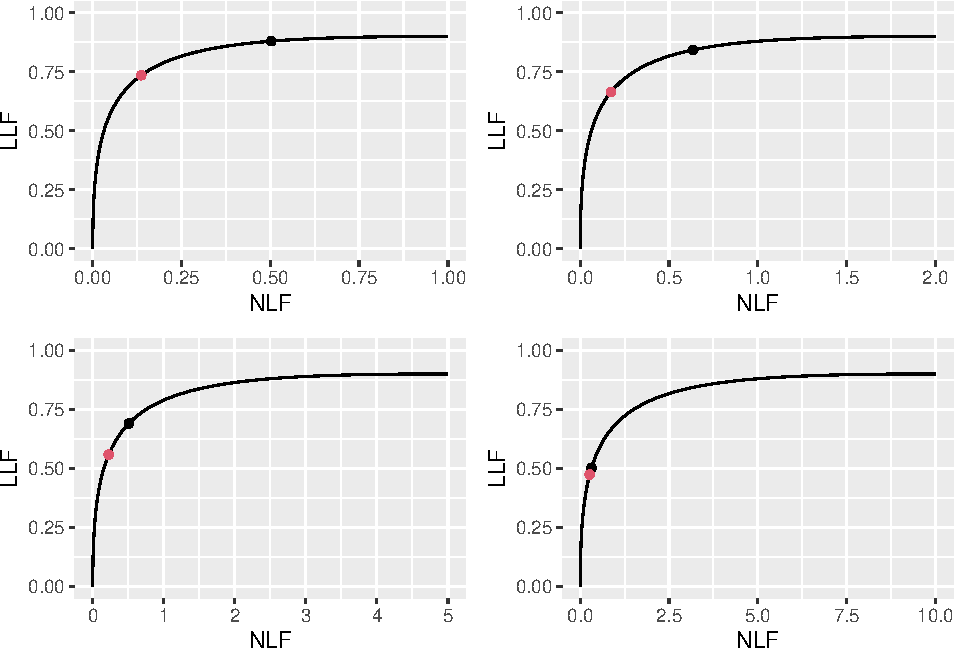
\includegraphics{21-optim-op-point-wafroc_files/figure-latex/optim-op-point-vary-lambda-froc-1.pdf}
\caption{\label{fig:optim-op-point-vary-lambda-froc}FROC plots with superimposed operating points for varying \(\lambda\). The red dot corresponds to \(\text{wAFROC}_\text{AUC}\) optimization and the black dot to Youden-index optimization.}
\end{figure}

\hypertarget{wafroc-1}{%
\subsection{wAFROC}\label{wafroc-1}}

Each wAFROC plot consists of a continuous curve followed by a dashed line. The ``red'' curve, corresponding to \(\text{wAFROC}_\text{AUC}\) optimization, appears as a ``solid-green solid-red dashed-red'' curve (the curve is in fact a true red curve complicated by superposition of the green curve over part of its traverse). The ``solid-green dashed-green'' curve corresponds to Youden-index optimization. As before the black dot denotes the Youden-index based operating point and the red dot denotes the \(\text{wAFROC}_\text{AUC}\) based operating point.

The transition from continuous to dashed is determined by the value of \(\zeta_1\). It occurs at a higher value of \(\zeta_1\) (lower transition point) for the Youden-index optimization. In other words the stricter Youden-index based threshold sacrifices some of the area under the wAFROC resulting in lower performance, particularly for the lower values of \(\lambda\). At the highest value of \(\lambda\) the values of optimal \(\zeta_1\) are similar and both methods make similar predictions.

\begin{figure}
\centering
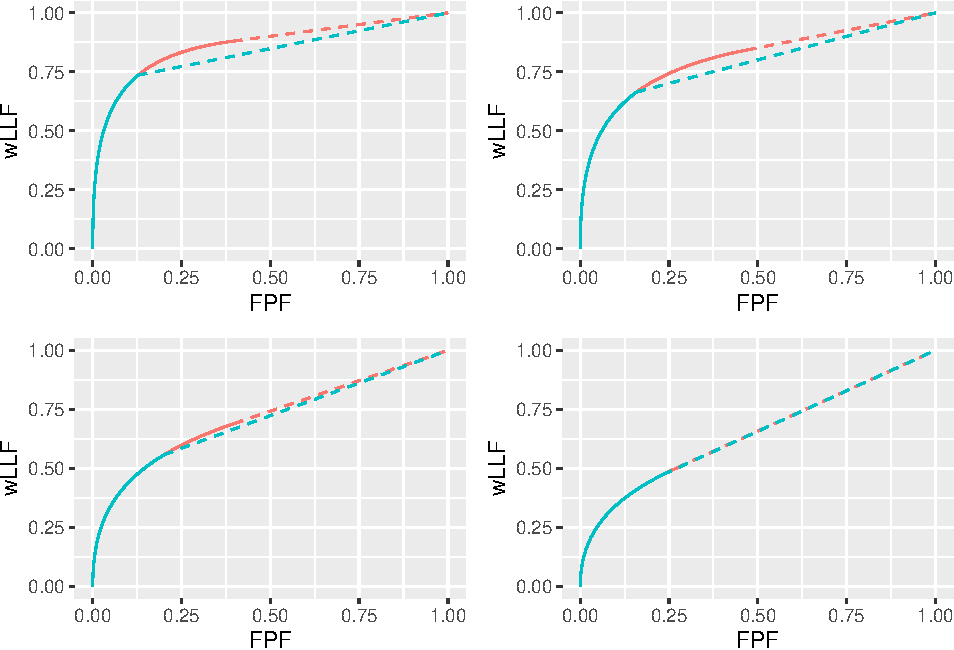
\includegraphics{21-optim-op-point-wafroc_files/figure-latex/optim-op-point-vary-lambda-wafroc-1.pdf}
\caption{\label{fig:optim-op-point-vary-lambda-wafroc}wAFROC plots for the two optimization methods: the ``solid-green solid-red dashed-red'' curve corresponds to \(\text{wAFROC}_\text{AUC}\) optimization and the ``solid-green dashed-green'' curve corresponds to Youden-index optimization. The \(\text{wAFROC}_\text{AUC}\) optimizations yield greater performance than do Youden-index optimizations and the difference decreases with increasing \(\lambda\).}
\end{figure}

\hypertarget{roc-1}{%
\subsection{ROC}\label{roc-1}}

The decrease in \(\text{ROC}_\text{AUC}\) with increasing \(\lambda\) is illustrated in Fig. \ref{fig:optim-op-point-vary-lambda-roc} which shows RSM-predicted ROC plots for the two optimization methods for the 4 values of \(\lambda\). Again, each plot consists of a continuous curve followed by a dashed curve and a similar color-coding convention is used as in Fig. \ref{fig:optim-op-point-vary-lambda-wafroc}. The ROC plots show similar dependencies as the wAFROC plots: the stricter Youden-index based reporting thresholds sacrifice some of the area under the ROC resulting in lower performance, particularly for the lower values of \(\lambda\).

\begin{figure}
\centering
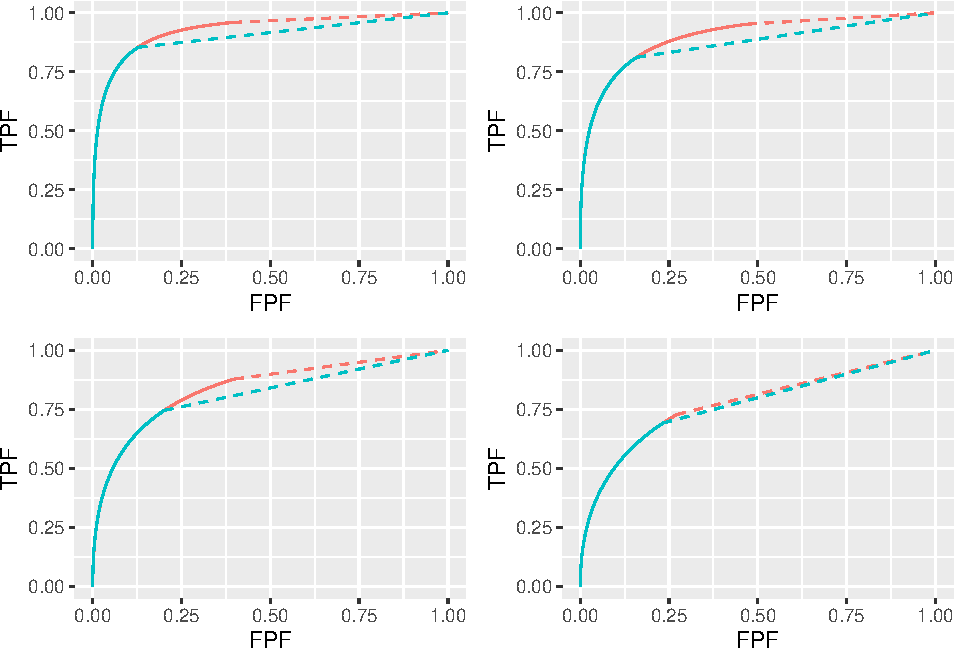
\includegraphics{21-optim-op-point-wafroc_files/figure-latex/optim-op-point-vary-lambda-roc-1.pdf}
\caption{\label{fig:optim-op-point-vary-lambda-roc}ROC plots for the two optimization methods: the ``solid-green solid-red dashed-red'' curve corresponds to \$ ext\{wAFROC\}\_ ext\{AUC\}\$ optimization and the ``solid-green dashed-green'' curve corresponds to Youden-index optimization. The \(\text{wAFROC}_\text{AUC}\) optimizations yield greater performance than Youden-index optimizations and the difference decreases with increasing \(\lambda\).}
\end{figure}

\hypertarget{why-not-maximize-roc-auc}{%
\subsection{Why not maximize ROC-AUC?}\label{why-not-maximize-roc-auc}}

Since the ROC curves show similarities to the wAFROC curves, why not maximize \(\text{ROC}_\text{AUC}\) instead of \(\text{wAFROC}_\text{AUC}\)? It can be shown that as long as one restricts to proper ROC models this always results in \(\zeta_1 = -\infty\), i.e., all latent marks are to be shown to the radiologist, an obviously incorrect strategy. This result can be understood from the following geometrical argument.

For a proper ROC curve the slope decreases monotonically as the operating point moves up the curve and at each point the slope is greater than that of the straight curve connecting the point to (1,1). This geometry ensures that AUC under any curve with a finite \(\zeta_1\) is smaller than that under the full curve. Therefore maximum AUC can only be attained by choosing \(\zeta_1 = -\infty\), see Fig. \ref{fig:binormal-model-threshold-dependence-2}.

\begin{figure}

{\centering 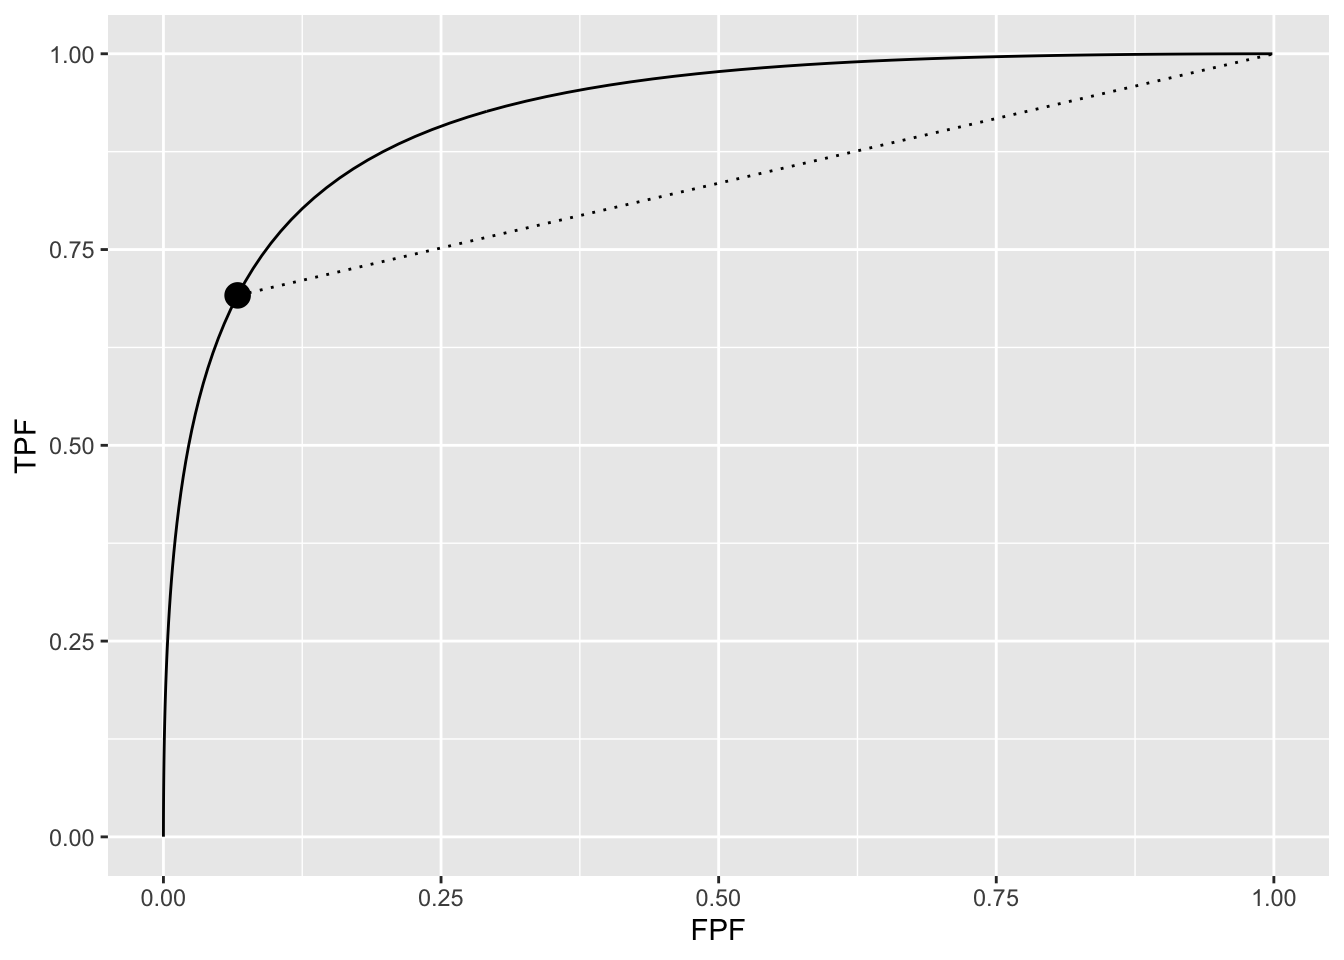
\includegraphics[width=300pt]{21-optim-op-point-wafroc_files/figure-latex/binormal-model-threshold-dependence-2-1} 

}

\caption{In the region above the dot the proper curve is above the dotted line, meaning that performance of an observer who adopts a finite $\zeta_1$ is less than performance of an observer who adopts $\zeta_1 = -\infty$.}\label{fig:binormal-model-threshold-dependence-2}
\end{figure}

\hypertarget{optim-op-point-vary-nu-mu}{%
\section{\texorpdfstring{Varying \(\nu\) and \(\mu\) optimizations}{Varying \textbackslash nu and \textbackslash mu optimizations}}\label{optim-op-point-vary-nu-mu}}

Details of varying \(\nu\) (with \(\mu\) and \(\lambda\) held constant) are in Appendix \ref{optim-op-point-vary-nu}. The results, summarized in Table \ref{tab:optim-op-point-table-vary-nu}, are similar to those just described for varying \(\lambda\) but, since unlike as was the case with increasing \(\lambda\), increasing \(\nu\) results in increasing performance, the \emph{directions of the effects are reversed}. For \(\text{wAFROC}_\text{AUC}\) optimization the optimal reporting threshold \(\zeta_1\) decreases with increasing \(\nu\). In contrast the Youden-index based optimal threshold is almost independent of \(\nu\). For \(\text{wAFROC}_\text{AUC}\) optimization the FROC operating point moves to higher NLF values while the Youden-index based operating point stays at a near constant NLF value, see Fig. \ref{fig:optim-op-point-vary-nu-froc}). As before, \(\text{wAFROC}_\text{AUC}\) optimizations yield higher performances than Youden-index optimizations (particularly for larger \(\nu\)): see Fig. \ref{fig:optim-op-point-vary-nu-wafroc} for the wAFROC and Fig. \ref{fig:optim-op-point-vary-nu-roc} for the ROC. The difference between the two optimization methods \emph{increases} with increasing \(\nu\) (for comparison the difference between the methods decreases with increasing \(\lambda\) -- this is what I meant by ``reversed effects'').

Details of varying \(\mu\) (with \(\lambda\) and \(\nu\) held constant) are in Appendix \ref{optim-op-point-vary-mu}. The results are summarized in Table \ref{tab:optim-op-point-table-vary-mu}. Increasing \(\mu\) is accompanied by increasing \(\zeta_1\) (i.e., stricter reporting threshold) and increasing \(\text{wAFROC}_\text{AUC}\) and \(\text{ROC}_\text{AUC}\). Performance measured either way is higher for \(\text{wAFROC}_\text{AUC}\) optimizations but the difference tends to shrink at the larger values of \(\mu\). LLF is relatively constant for \(\text{wAFROC}_\text{AUC}\) optimizations while it increases slowly with \(\mu\) for Youden-index optimizations. NLF decreases with increasing \(\mu\) for both optimization methods, i.e, the FROC operating point shifts leftward, see Fig. \ref{fig:optim-op-point-vary-mu-froc}). Again, \(\text{wAFROC}_\text{AUC}\) optimization yields a lower reporting threshold and higher performance than Youden-index optimization, see Fig. \ref{fig:optim-op-point-vary-mu-wafroc} for the wAFROC and Fig. \ref{fig:optim-op-point-vary-mu-roc} for the ROC. The difference between the two optimization methods decreases with increasing \(\mu\).

\hypertarget{optim-op-point-vary-nu-limiting-situations}{%
\section{Limiting situations}\label{optim-op-point-vary-nu-limiting-situations}}

Limiting situations covering high and low performances are described in \ref{optim-op-point-limiting-situations}.

For high performance, defined as \(\text{ROC}_\text{AUC} > 0.9\), both methods place the optimal operating point near the inflection point on the upper-left corner of the wAFROC or ROC. The \(\text{wAFROC}_\text{AUC}\) based method chooses a lower threshold than the Youden-index method resulting in a higher operating point on the FROC and higher \(\text{wAFROC}_\text{AUC}\) and \(\text{ROC}_\text{AUC}\). The difference between the two methods decreases as \(\text{ROC}_\text{AUC} \rightarrow 1\).

For low performance, defined as \(0.5 < \text{ROC}_\text{AUC} < 0.6\), the Youden-index method selected a lower threshold compared to \(\text{wAFROC}_\text{AUC}\) optimization, resulting in a higher operating point on the FROC, greater \(\text{ROC}_\text{AUC}\) but sharply lower \(\text{wAFROC}_\text{AUC}\). The difference between the two methods increases as \(\text{ROC}_\text{AUC} \rightarrow 0.5\). In this limit the \(\text{wAFROC}_\text{AUC}\) method severely limits the numbers of marks shown to the radiologist as compared to the Youden-index based method.

\hypertarget{optim-op-point-trends}{%
\section{Trends}\label{optim-op-point-trends}}

No matter how the RSM parameters are varied the trend is that \(\text{wAFROC}_\text{AUC}\) optimizations result in lower optimal thresholds \(\zeta_1\) (i.e.,laxer reporting criteria that result in more displayed marks) than Youden-index optimizations. Accordingly the \(\text{wAFROC}_\text{AUC}\) optimizations yield FROC operating points at higher NLF values (i.e., red dots to the right of the black dots in FROC plots), greater \(\text{wAFROC}_\text{AUC}\)s (red curves above the green curves in wAFROC plots) and greater \(\text{ROC}_\text{AUC}\)s (red curves above the green curves in ROC plots). These trends are true no matter how the RSM parameters are varied provided CAD performance is not too low.

If CAD performance is very low there are instructive exceptions where \(\text{wAFROC}_\text{AUC}\) optimizations yield \emph{greater} \(\zeta_1\) (i.e., stricter reporting criteria that result in \emph{fewer} displayed marks) than Youden-index optimizations. This finding is true no matter how the RSM parameters are varied.

Consider for example the low performance varying \(\nu\) optimizations described in Appendix \ref{optim-op-point-low-performance-vary-nu}. The FROC plots, Fig. \ref{fig:optim-op-point-low-performance-vary-nu-froc}, corresponding to \(\mu = 1\), \(\lambda = 10\), \(\nu = 0.1, 0.2, 0.3, 0.4\), show that the \(\text{wAFROC}_\text{AUC}\) optimal operating points are very close to the origin \(\text{NLF} = 0\), i.e., very few marks are displayed. In contrast the Youden-index optimal operating points are shifted towards larger \(\text{NLF}\) values allowing more marks to be displayed. The wAFROC plots, Fig. \ref{fig:optim-op-point-low-performance-vary-nu-wafroc}, show a large difference in AUCs between the two methods, especially for the smaller values of \(\nu\): for example, for \(\nu=0.1\), the \(\text{wAFROC}_\text{AUC}\) corresponding to \(\text{wAFROC}_\text{AUC}\) optimization is 0.5000002 while that corresponding to Youden-index optimization is 0.2923394. Clearly the \(\text{wAFROC}_\text{AUC}\) optimization yields a larger \(\text{wAFROC}_\text{AUC}\) relative to Youden-index optimization, which it must as \(\text{wAFROC}_\text{AUC}\) is the quantity being optimized.

While Youden-index optimizations yield smaller \(\text{wAFROC}_\text{AUC}\) values they do yield larger \(\text{ROC}_\text{AUC}\) values as is evident by comparing the ROC plots, Fig. \ref{fig:optim-op-point-low-performance-vary-nu-roc}. For \(\nu=0.1\) the \(\text{ROC}_\text{AUC}\) corresponding to \(\text{wAFROC}_\text{AUC}\) optimization is 0.5000024 while that corresponding to Youden-index optimization is 0.5143474. Clearly \(\text{wAFROC}_\text{AUC}\) optimization yields a very close to chance-level \(\text{ROC}_\text{AUC}\) while Youden-index optimization yields a slightly larger \(\text{ROC}_\text{AUC}\).

Keep in mind that \(\text{ROC}_\text{AUC}\) measures classification accuracy performance between non-diseased and diseased cases: it does not care about lesion localization accuracy. In contrast \(\text{wAFROC}_\text{AUC}\) measures both lesion localization accuracy and lesion classification accuracy. By choosing an optimal operating point close to the origin the low performance CAD does not get credit for missing almost all the lesions on diseased cases but it does get credit for not marking non-diseased cases.

\hypertarget{optim-op-point-how-to-use-method}{%
\section{Applying the method}\label{optim-op-point-how-to-use-method}}

Assume that one has designed an algorithmic observer that has been optimized with respect to all other parameters except the reporting threshold. At this point the algorithm reports every suspicious region no matter how low the malignancy index. The mark-rating pairs are entered into a \texttt{RJafroc} format Excel input file, as describe \href{https://dpc10ster.github.io/RJafrocQuickStart/quick-start-froc-data-format.html}{here}. The next step is to read the data file -- \texttt{DfReadDataFile()} -- convert it to an ROC dataset -- \texttt{DfFroc2Roc()} -- and then perform a radiological search model (RSM) fit to the dataset using function \texttt{FitRsmRoc()}. This yields the necessary \(\lambda, \mu, \nu\) parameters. These values are used to perform the computations described in this chapter to determine the optimal reporting threshold. The RSM parameter values and the reporting threshold determine the optimal reporting point on the FROC curve. The designer sets the algorithm to only report marks with confidence levels exceeding this threshold. These steps are illustrated in the following example.

\hypertarget{optim-op-point-application}{%
\subsection{A CAD application}\label{optim-op-point-application}}

Not having access to any CAD FROC datasets the standalone CAD LROC dataset described in \citep{hupse2013standalone} was used to create a simulated FROC (i.e., \(\text{ROC}_\text{AUC}\) equivalent) dataset which is embedded in \texttt{RJafroc} as object \texttt{datasetCadSimuFroc}. In the following code the first reader for this dataset, corresponding to CAD, is extracted using \texttt{DfExtractDataset} (the other reader data, corresponding to radiologists, are ignored). The function \texttt{DfFroc2Roc} converts \texttt{dsCad} to an ROC dataset. The function \texttt{DfBinDataset} bins the data to about 7 bins. Each diseased case contains one lesion: \texttt{lesDistr\ =\ c(1)}. \texttt{FitRsmRoc} fits the binned ROC dataset to the radiological search model (RSM). Object \texttt{fit} contains the RSM parameters required to perform the optimizations described in previous sections.

\begin{Shaded}
\begin{Highlighting}[]
\NormalTok{ds }\OtherTok{\textless{}{-}}\NormalTok{ RJafroc}\SpecialCharTok{::}\NormalTok{datasetCadSimuFroc}
\NormalTok{dsCad }\OtherTok{\textless{}{-}}\NormalTok{ RJafroc}\SpecialCharTok{::}\FunctionTok{DfExtractDataset}\NormalTok{(ds, }\AttributeTok{rdrs =} \DecValTok{1}\NormalTok{)}
\NormalTok{dsCadRoc }\OtherTok{\textless{}{-}}\NormalTok{ RJafroc}\SpecialCharTok{::}\FunctionTok{DfFroc2Roc}\NormalTok{(dsCad)}
\NormalTok{dsCadRocBinned }\OtherTok{\textless{}{-}}\NormalTok{ RJafroc}\SpecialCharTok{::}\FunctionTok{DfBinDataset}\NormalTok{(dsCadRoc, }\AttributeTok{opChType =} \StringTok{"ROC"}\NormalTok{)}
\NormalTok{lesDistrCad }\OtherTok{\textless{}{-}} \FunctionTok{c}\NormalTok{(}\DecValTok{1}\NormalTok{) }\CommentTok{\# LROC dataset has one lesion per diseased case}
\NormalTok{relWeightsCad }\OtherTok{\textless{}{-}} \FunctionTok{c}\NormalTok{(}\DecValTok{1}\NormalTok{)}
\NormalTok{fit }\OtherTok{\textless{}{-}}\NormalTok{ RJafroc}\SpecialCharTok{::}\FunctionTok{FitRsmRoc}\NormalTok{(dsCadRocBinned, lesDistrCad)}
\FunctionTok{cat}\NormalTok{(}\FunctionTok{sprintf}\NormalTok{(}\StringTok{"fitted values: mu = \%5.3f,"}\NormalTok{, fit}\SpecialCharTok{$}\NormalTok{mu), }
    \FunctionTok{sprintf}\NormalTok{(}\StringTok{"lambda = \%5.3f,"}\NormalTok{, fit}\SpecialCharTok{$}\NormalTok{lambda), }
    \FunctionTok{sprintf}\NormalTok{(}\StringTok{"nu = \%5.3f."}\NormalTok{, fit}\SpecialCharTok{$}\NormalTok{nu)) }
\CommentTok{\#\textgreater{} fitted values: mu = 2.756, lambda = 6.778, nu = 0.803.}
\end{Highlighting}
\end{Shaded}

\hypertarget{summary-table-1}{%
\subsubsection{Summary table}\label{summary-table-1}}

Table \ref{tab:optim-op-point-table4} summarizes the results. As compared to Youden-index optimization the \(\text{wAFROC}_\text{AUC}\) based optimization results in a lower reporting threshold \(\zeta_1\), larger figures of merit -- see Fig. \ref{fig:optim-op-point-application-wafroc} for \(\text{wAFROC}_\text{AUC}\) and Fig. \ref{fig:optim-op-point-application-roc} for \(\text{ROC}_\text{AUC}\) -- and a higher operating point on the FROC, see Fig. \ref{fig:optim-op-point-application-froc}. These results match the trends shown in Table \ref{tab:optim-op-point-table-vary-lambda}.

\begin{table}

\caption{\label{tab:optim-op-point-table4}Results for example CAD FROC dataset. Table header row as in the previous table.}
\centering
\fontsize{10}{12}\selectfont
\begin{tabular}[t]{llllll}
\toprule
FOM & $\lambda$ & $\zeta_1$ & $\text{wAFROC}$ & $\text{ROC}$ & $\left( \text{NLF}, \text{LLF}\right)$\\
\midrule
wAFROC & 6.778 & 1.739 & 0.774 & 0.815 & (0.278, 0.679)\\
Youden &  & 1.982 & 0.770 & 0.798 & (0.161, 0.627)\\
\bottomrule
\end{tabular}
\end{table}

\hypertarget{froc-2}{%
\subsubsection{FROC}\label{froc-2}}

Fig. \ref{fig:optim-op-point-application-froc} shows FROC curves with superimposed optimal operating points. With NLF = 0.278, a four-view mammogram would show about 1.2 false CAD marks per patient and lesion-level sensitivity would be about 68 percent.

\begin{figure}

{\centering 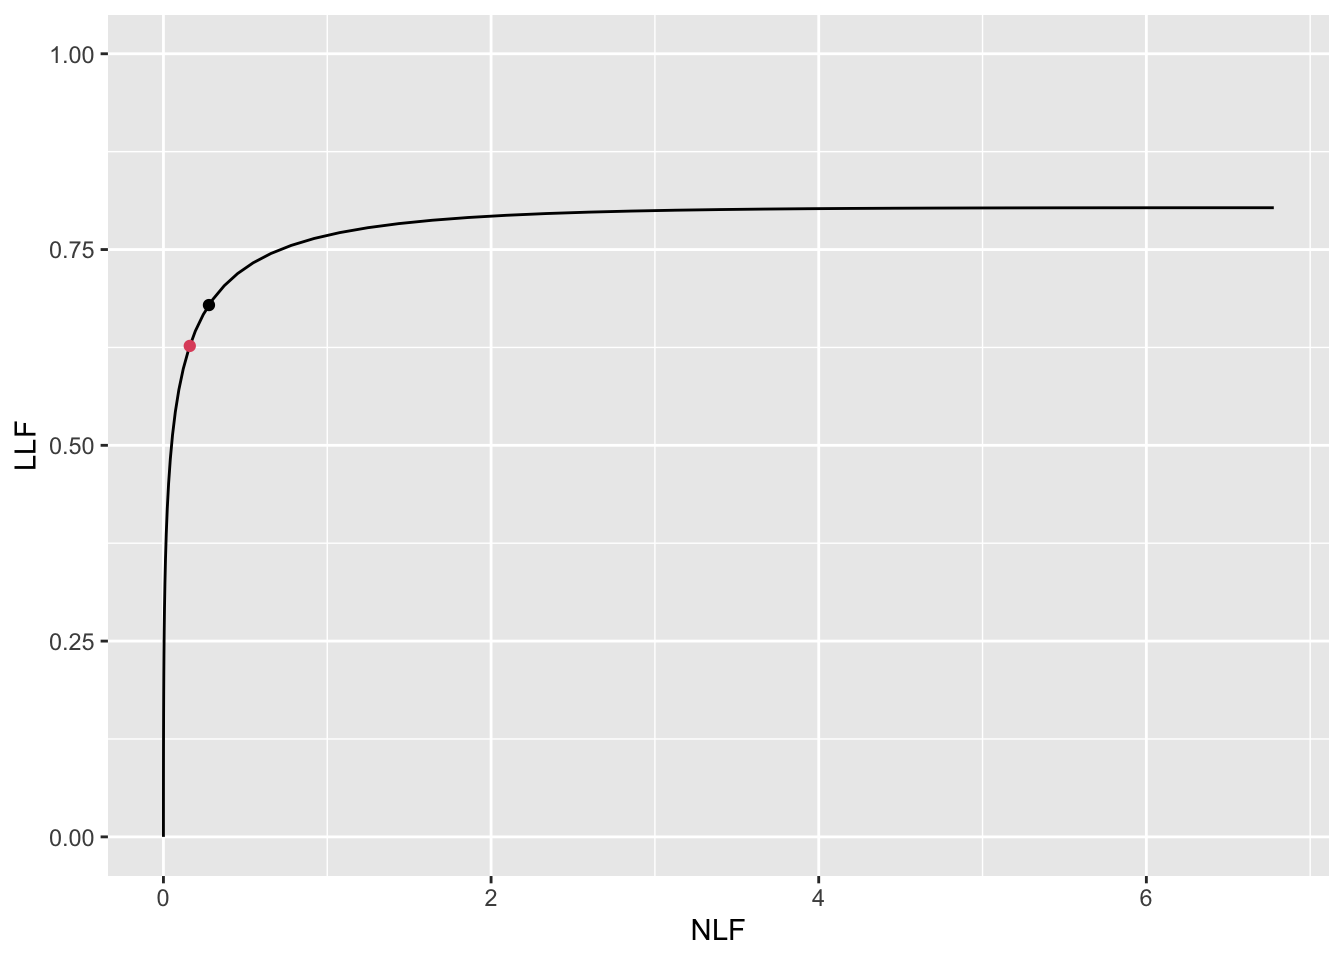
\includegraphics[width=300pt]{21-optim-op-point-wafroc_files/figure-latex/optim-op-point-application-froc-1} 

}

\caption{FROC plots with superposed optimal operating points. The red dot is using $\text{wAFROC}_\text{AUC}$ optimization and black dot is using Youden-index optimization.}\label{fig:optim-op-point-application-froc}
\end{figure}

\hypertarget{wafroc-2}{%
\subsubsection{wAFROC}\label{wafroc-2}}

Fig. \ref{fig:optim-op-point-application-wafroc} shows wAFROC curves using the two methods. The red curve is using \(\text{wAFROC}_\text{AUC}\) optimization and the green curve is using Youden-index optimization. The difference in AUCs is small - following the trend described in Appendix \ref{optim-op-point-vary-nu-mu} for the larger values of \(\lambda\).

\begin{figure}

{\centering 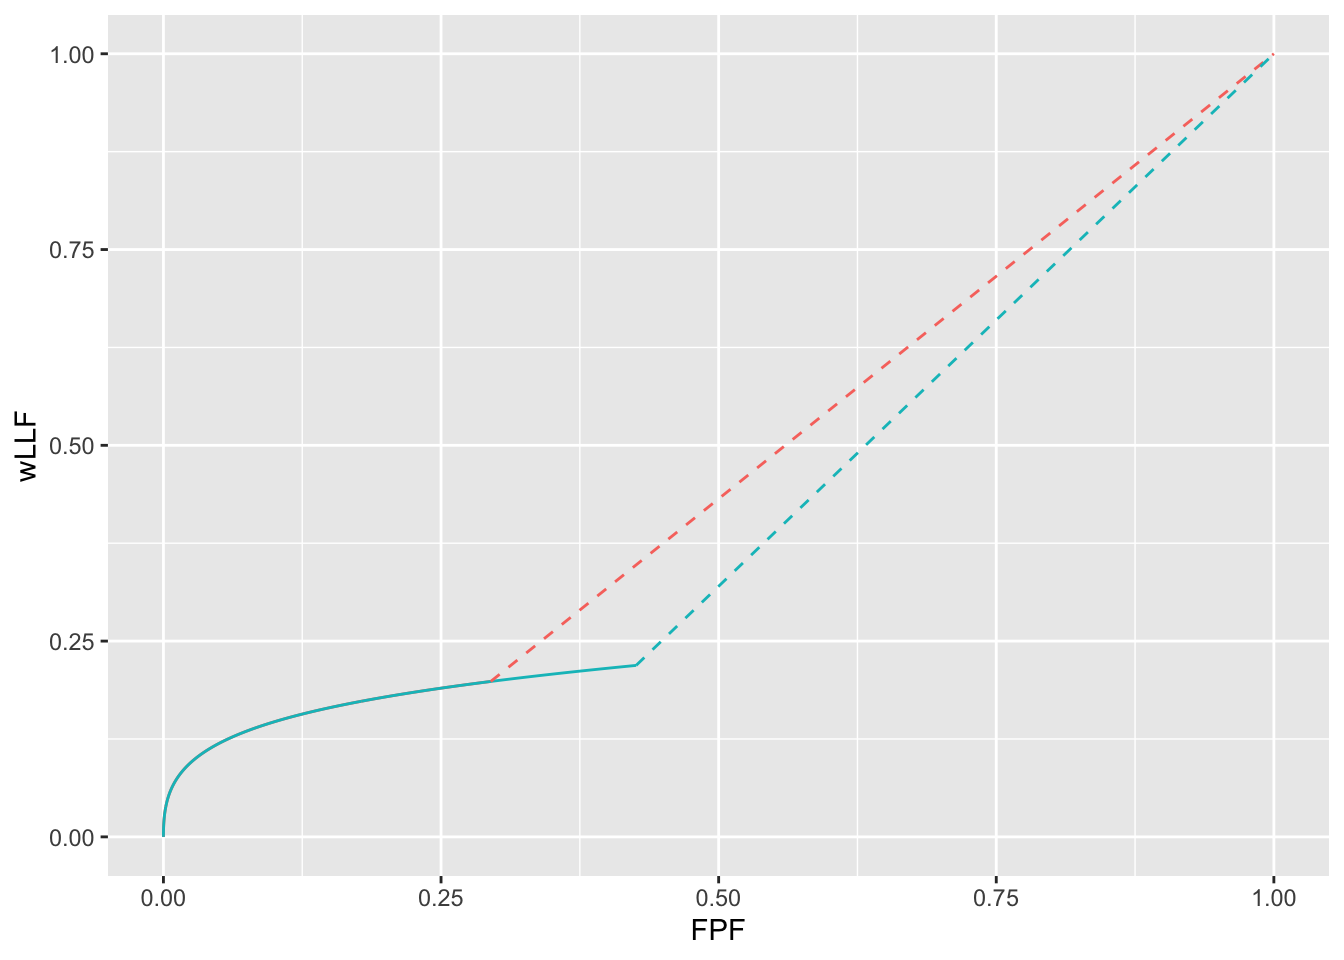
\includegraphics[width=300pt]{21-optim-op-point-wafroc_files/figure-latex/optim-op-point-application-wafroc-1} 

}

\caption{The color coding is as in previous figures. The two $\text{wAFROC}_\text{AUC}$s are 0.774 (wAFROC optimization) and 0.770 (Youden-index optimization).}\label{fig:optim-op-point-application-wafroc}
\end{figure}

\hypertarget{roc-2}{%
\subsubsection{ROC}\label{roc-2}}

Fig. \ref{fig:optim-op-point-application-roc} shows ROC curves using the two methods. The red curve is using \(\text{wAFROC}_\text{AUC}\) optimization and the green curve is using Youden-index optimization.

\begin{figure}

{\centering 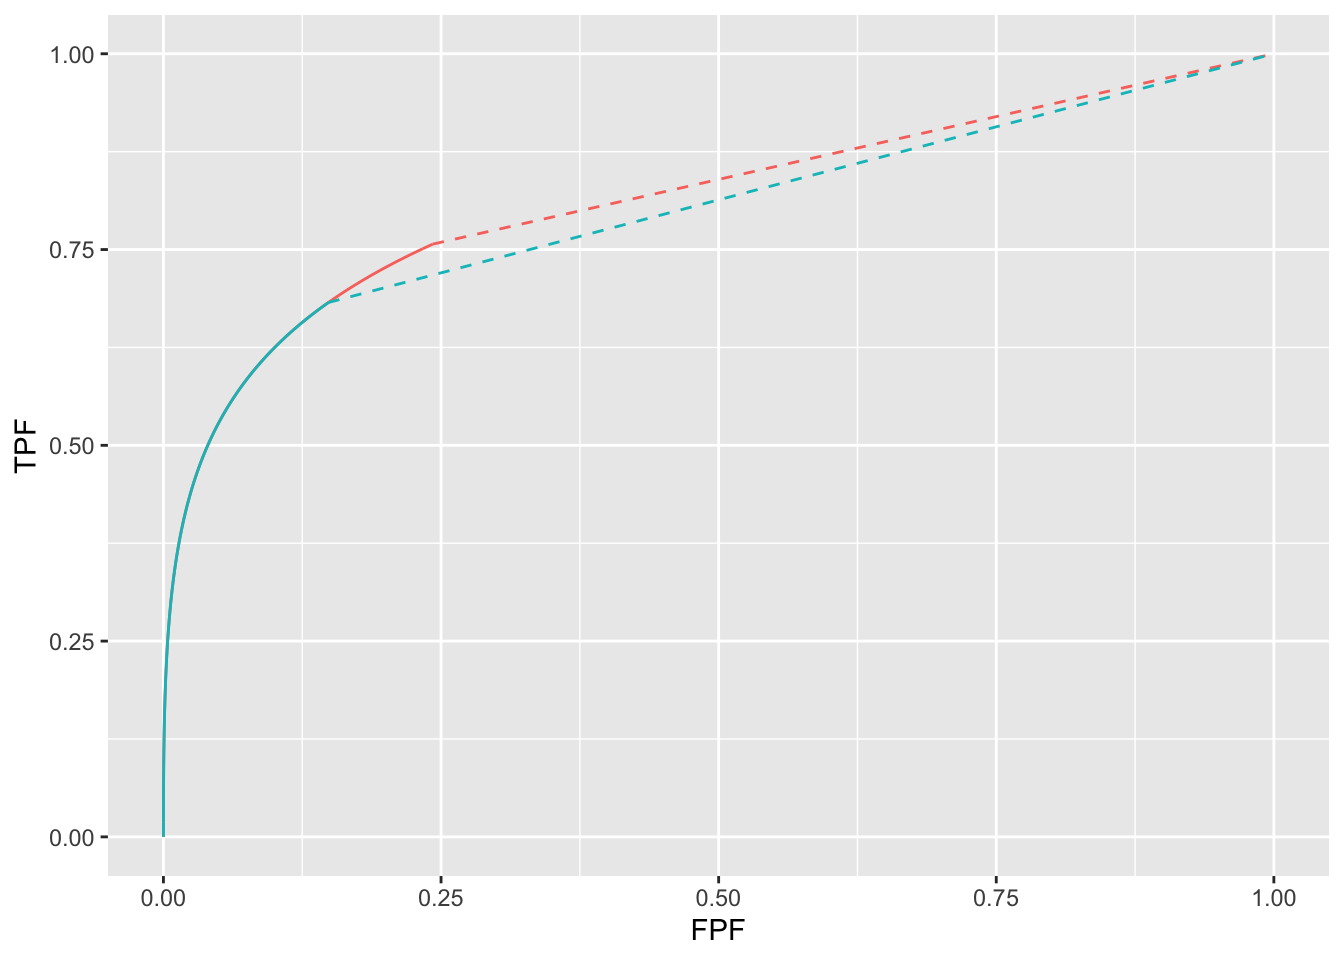
\includegraphics[width=300pt]{21-optim-op-point-wafroc_files/figure-latex/optim-op-point-application-roc-1} 

}

\caption{The color coding is as in previous figures. The two $\text{ROC}_\text{AUC}$s are 0.815 (wAFROC optimization) and 0.798 (Youden-index optimization).}\label{fig:optim-op-point-application-roc}
\end{figure}

\hypertarget{optim-op-point-discussion}{%
\section{TBA Discussion}\label{optim-op-point-discussion}}

\begin{Shaded}
\begin{Highlighting}[]
\NormalTok{muArr }\OtherTok{\textless{}{-}} \FunctionTok{c}\NormalTok{(}\DecValTok{2}\NormalTok{)}
\NormalTok{lambdaArr }\OtherTok{\textless{}{-}} \FunctionTok{c}\NormalTok{(}\DecValTok{1}\NormalTok{, }\DecValTok{2}\NormalTok{, }\DecValTok{5}\NormalTok{, }\DecValTok{10}\NormalTok{)}
\NormalTok{nuArr }\OtherTok{\textless{}{-}} \FunctionTok{c}\NormalTok{(}\FloatTok{0.9}\NormalTok{)}
\NormalTok{lesDistr }\OtherTok{\textless{}{-}} \FunctionTok{c}\NormalTok{(}\FloatTok{0.5}\NormalTok{, }\FloatTok{0.5}\NormalTok{)}
\NormalTok{relWeights }\OtherTok{\textless{}{-}} \FunctionTok{c}\NormalTok{(}\FloatTok{0.5}\NormalTok{, }\FloatTok{0.5}\NormalTok{)}
\FunctionTok{source}\NormalTok{(}\StringTok{"R/optim{-}op{-}point/doOneTable.R"}\NormalTok{, }\AttributeTok{local =}\NormalTok{ knitr}\SpecialCharTok{::}\FunctionTok{knit\_global}\NormalTok{())}
\end{Highlighting}
\end{Shaded}

In Table \ref{tab:optim-op-point-table-vary-lambda} the \(\lambda\) parameter controls the average number of perceived NLs per case. For \(\lambda = 1\) there is, on average, one perceived NL for every case and the optimal \(\text{wAFROC}_\text{AUC}\) based threshold is \(\zeta_1\) = -0.007. For \(\lambda = 10\) there are ten perceived NLs for every case and the optimal \(\text{wAFROC}_\text{AUC}\) based threshold is \(\zeta_1\) = 1.856. The reason for the increase in \(\zeta_1\) should be obvious: with increasing numbers of latent NLs (perceived false marks) per case it is necessary to adopt a stricter criteria because otherwise the reader would be shown 10 times the number of false marks per case.

The \(\text{ROC}_\text{AUC}\)s are reported as a check of the less familiar \(\text{wAFROC}_\text{AUC}\) figure of merit. With some notable exceptions the behavior of the two optimization methods is independent of whether it is measured via the \(\text{wAFROC}_\text{AUC}\) or the \(\text{ROC}_\text{AUC}\): either way the \(\text{wAFROC}_\text{AUC}\) optimizations yield higher AUC values and higher operating points on the FROC than the corresponding Youden-index optimizations. The exceptions occur when CAD performance is very low in which situation the .

In this example the difference in \(\text{wAFROC}_\text{AUC}\), \(\text{ROC}_\text{AUC}\) and the operating points between the two methods decreases as performance \emph{increases}, which is the opposite of that found when \(\lambda\) or \(\nu\) were varied. With constant \(\lambda\) and \(\nu\) the \emph{numbers} of latent NLs and LLs are unchanging; all that happens is the \emph{values} of the z-samples from LLs increase as \(\mu\) increases, which allows the optimal threshold to increase (this can be understood as a ``ROC-paradigm'' effect: as the normal distributions are more widely separated, the optimal threshold will increase, approaching, in the limit, half the separation, since in that limit TPF = 1 and FPF = 0).

This is due to two reinforcing effects: performance goes down with increasing numbers of NLs per case and performance goes down with increasing optimal reporting threshold (see \ref{rsm-predictions-roc-curve-aucs-zeta1} for explanation of the \(\zeta_1\) dependence of AUC performance). It is difficult to unambiguously infer performance based on the FROC operating points: as \(\lambda\) increases LLF decreases but for \(\text{wAFROC}_\text{AUC}\) optimizations NLF peaks while for Youden-index optimizations it increases.

The FROC plots also illustrate the decrease in \(\text{LLF}\) with increasing \(\lambda\): the black dots move to smaller ordinates, as do the red dots, which would seem to imply decreasing performance. However, the accompanying change in \(\text{NLF}\) rules out an unambiguous determination of the direction of the change in overall performance based on the FROC curve.

For very low performance, defined as \(0.5 < \text{ROC}_\text{AUC} < 0.6\), the Youden-index method chooses a lower threshold compared to \(\text{wAFROC}_\text{AUC}\) optimization, resulting in a higher operating point on the FROC, greater \(\text{ROC}_\text{AUC}\) but sharply lower \(\text{wAFROC}_\text{AUC}\). The difference between the two methods increases as \(\text{ROC}_\text{AUC} \rightarrow 0.5\). In this limit the \(\text{wAFROC}_\text{AUC}\) method severely limits the numbers of marks shown to the radiologist as compared to the Youden-index based method.

\hypertarget{cad-optim-op-appendices}{%
\section{Appendices}\label{cad-optim-op-appendices}}

\hypertarget{optim-op-point-vary-nu}{%
\subsection{\texorpdfstring{Varying \(\nu\) optimizations}{Varying \textbackslash nu optimizations}}\label{optim-op-point-vary-nu}}

For \(\mu = 2\) and \(\lambda = 1\) optimizations were performed for \(\nu = 0.6, 0.7, 0.8, 0.9\).

\begin{Shaded}
\begin{Highlighting}[]
\NormalTok{muArr }\OtherTok{\textless{}{-}} \FunctionTok{c}\NormalTok{(}\DecValTok{2}\NormalTok{)}
\NormalTok{lambdaArr }\OtherTok{\textless{}{-}} \FunctionTok{c}\NormalTok{(}\DecValTok{1}\NormalTok{)}
\NormalTok{nuArr }\OtherTok{\textless{}{-}} \FunctionTok{c}\NormalTok{(}\FloatTok{0.6}\NormalTok{, }\FloatTok{0.7}\NormalTok{, }\FloatTok{0.8}\NormalTok{, }\FloatTok{0.9}\NormalTok{)}
\NormalTok{lesDistr }\OtherTok{\textless{}{-}} \FunctionTok{c}\NormalTok{(}\FloatTok{0.5}\NormalTok{, }\FloatTok{0.5}\NormalTok{)}
\NormalTok{relWeights }\OtherTok{\textless{}{-}} \FunctionTok{c}\NormalTok{(}\FloatTok{0.5}\NormalTok{, }\FloatTok{0.5}\NormalTok{)}
\end{Highlighting}
\end{Shaded}

\hypertarget{summary-table-2}{%
\subsubsection{Summary table}\label{summary-table-2}}

\begin{table}

\caption{\label{tab:optim-op-point-table-vary-nu}Results for $\mu = 2$, $\lambda = 1$ and varying $\nu$.}
\centering
\fontsize{10}{12}\selectfont
\begin{tabular}[t]{llllll}
\toprule
FOM & $\nu$ & $\zeta_1$ & $\text{wAFROC}_\text{AUC}$ & $\text{ROC}_\text{AUC}$ & $\left( \text{NLF}, \text{LLF}\right)$\\
\midrule
$\text{wAFROC}_\text{AUC}$ & 0.6 & 0.888 & 0.701 & 0.804 & (0.187, 0.520)\\
 & 0.7 & 0.674 & 0.751 & 0.851 & (0.250, 0.635)\\
 & 0.8 & 0.407 & 0.805 & 0.893 & (0.342, 0.756)\\
 & 0.9 & -0.007 & 0.864 & 0.929 & (0.503, 0.880)\\
Youden-index & 0.6 & 1.022 & 0.700 & 0.797 & (0.153, 0.502)\\
\addlinespace
 & 0.7 & 1.044 & 0.745 & 0.835 & (0.148, 0.581)\\
 & 0.8 & 1.069 & 0.788 & 0.868 & (0.143, 0.659)\\
 & 0.9 & 1.095 & 0.831 & 0.899 & (0.137, 0.735)\\
\bottomrule
\end{tabular}
\end{table}

\hypertarget{froc-3}{%
\subsubsection{FROC}\label{froc-3}}

\begin{figure}
\centering
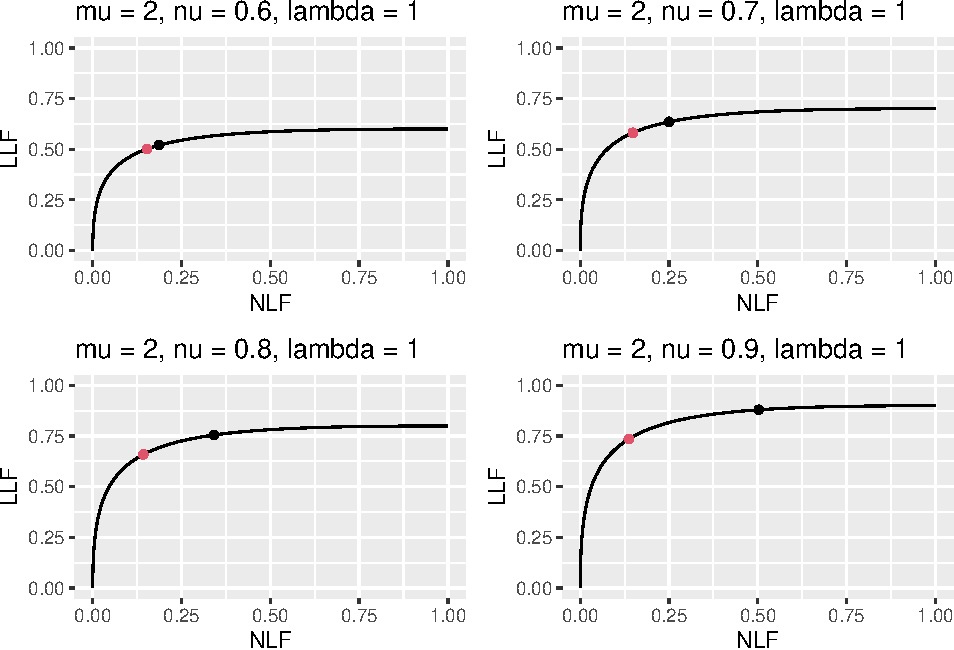
\includegraphics{21-optim-op-point-wafroc_files/figure-latex/optim-op-point-vary-nu-froc-1.pdf}
\caption{\label{fig:optim-op-point-vary-nu-froc}Varying \(\nu\) FROC plots with superimposed operating points. The red dot corresponds to \(\text{wAFROC}_\text{AUC}\) optimization and the black dot to Youden-index optimization. The values of \(\nu\) are: top-left \(\nu = 0.6\), top-right \(\nu = 0.7\), bottom-left \(\nu = 0.8\) and bottom-right \(\nu = 0.9\). Each red dot is above the corresponding black dot and their separation increases as \(\nu\) increases, i.e., as CAD performance increases.}
\end{figure}

\hypertarget{wafroc-3}{%
\subsubsection{wAFROC}\label{wafroc-3}}

\begin{figure}
\centering
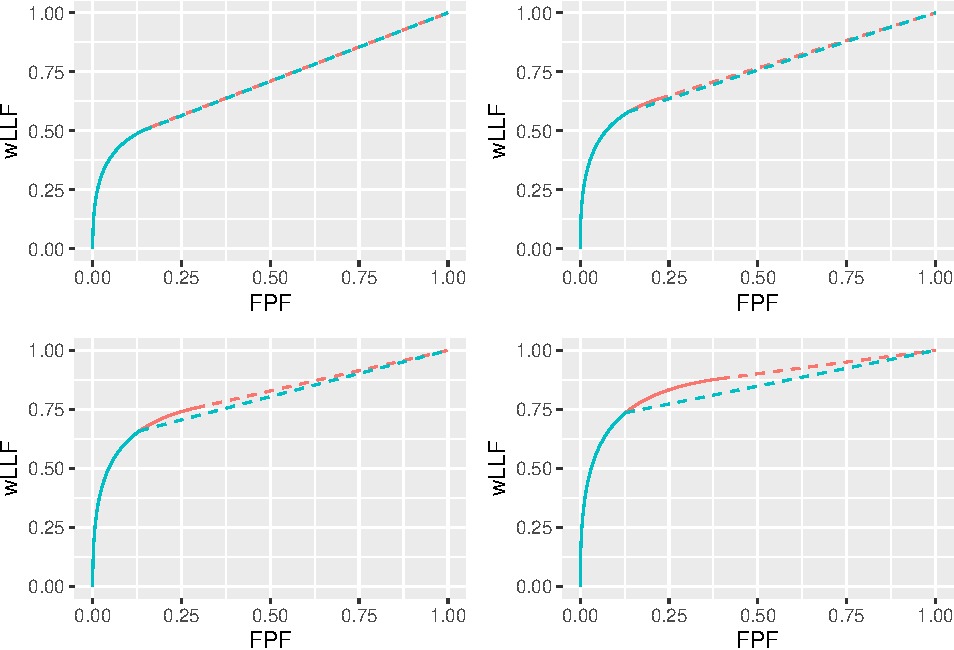
\includegraphics{21-optim-op-point-wafroc_files/figure-latex/optim-op-point-vary-nu-wafroc-1.pdf}
\caption{\label{fig:optim-op-point-vary-nu-wafroc}Varying \(\nu\) wAFROC plots for the two optimization methods with superimposed operating points with superimposed operating points. The color coding is as in previous figures. The values of \(\nu\) are: top-left \(\nu = 0.6\), top-right \(\nu = 0.7\), bottom-left \(\nu = 0.8\) and bottom-right \(\nu = 0.9\).}
\end{figure}

\hypertarget{roc-3}{%
\subsubsection{ROC}\label{roc-3}}

\begin{figure}
\centering
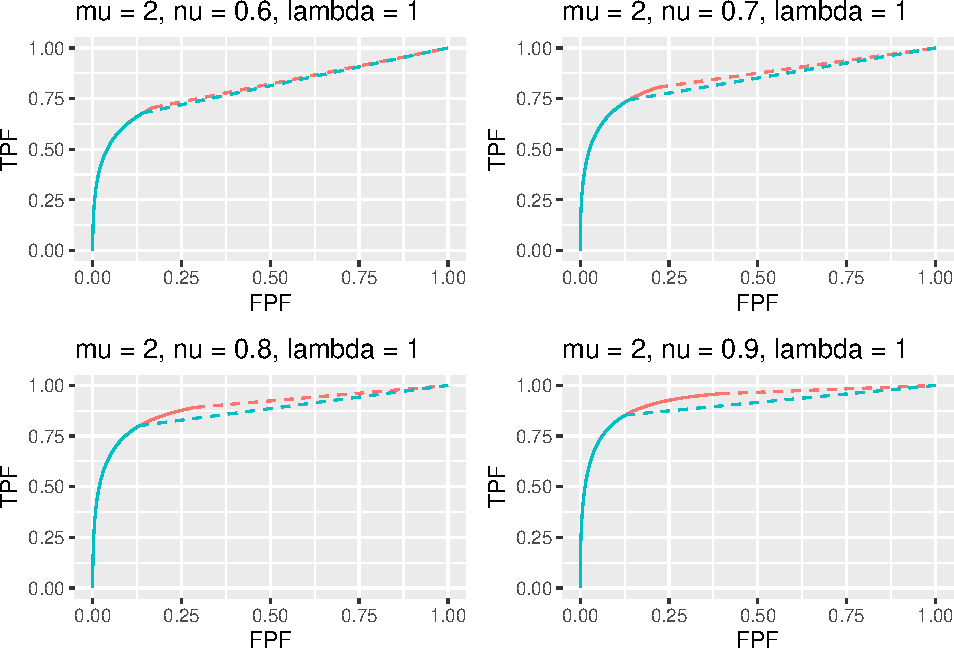
\includegraphics{21-optim-op-point-wafroc_files/figure-latex/optim-op-point-vary-nu-roc-1.pdf}
\caption{\label{fig:optim-op-point-vary-nu-roc}Varying \(\nu\) ROC plots for the two optimization methods with superimposed operating points with superimposed operating points. The color coding is as in previous figures. The values of \(\nu\) are: top-left \(\nu = 0.6\), top-right \(\nu = 0.7\), bottom-left \(\nu = 0.8\) and bottom-right \(\nu = 0.9\).}
\end{figure}

\hypertarget{optim-op-point-vary-mu}{%
\subsection{\texorpdfstring{Varying \(\mu\) optimizations}{Varying \textbackslash mu optimizations}}\label{optim-op-point-vary-mu}}

For \(\lambda = 1\) and \(\nu = 0.9\) optimizations were performed for \(\mu = 1, 2, 3, 4\).

\begin{Shaded}
\begin{Highlighting}[]
\NormalTok{muArr }\OtherTok{\textless{}{-}} \FunctionTok{c}\NormalTok{(}\DecValTok{1}\NormalTok{, }\DecValTok{2}\NormalTok{, }\DecValTok{3}\NormalTok{, }\DecValTok{4}\NormalTok{)}
\NormalTok{lambdaArr }\OtherTok{\textless{}{-}} \DecValTok{1}
\NormalTok{nuArr }\OtherTok{\textless{}{-}} \FloatTok{0.9}
\end{Highlighting}
\end{Shaded}

\hypertarget{summary-table-3}{%
\subsubsection{Summary table}\label{summary-table-3}}

\begin{table}

\caption{\label{tab:optim-op-point-table-vary-mu}Results for $\lambda = 1$, $\nu = 0.9$ and varying $\mu$.}
\centering
\fontsize{10}{12}\selectfont
\begin{tabular}[t]{llllll}
\toprule
FOM & $\mu$ & $\zeta_1$ & $\text{wAFROC}_\text{AUC}$ & $\text{ROC}_\text{AUC}$ & $\left( \text{NLF}, \text{LLF}\right)$\\
\midrule
$\text{wAFROC}_\text{AUC}$ & 1 & -1.663 & 0.745 & 0.850 & (0.952, 0.897)\\
 & 2 & -0.007 & 0.864 & 0.929 & (0.503, 0.880)\\
 & 3 & 0.808 & 0.922 & 0.961 & (0.210, 0.887)\\
 & 4 & 1.463 & 0.942 & 0.970 & (0.072, 0.895)\\
Youden-index & 1 & 0.462 & 0.704 & 0.815 & (0.322, 0.634)\\
\addlinespace
 & 2 & 1.095 & 0.831 & 0.899 & (0.137, 0.735)\\
 & 3 & 1.629 & 0.903 & 0.945 & (0.052, 0.823)\\
 & 4 & 2.124 & 0.935 & 0.964 & (0.017, 0.873)\\
\bottomrule
\end{tabular}
\end{table}

\hypertarget{froc-4}{%
\subsubsection{FROC}\label{froc-4}}

\begin{figure}
\centering
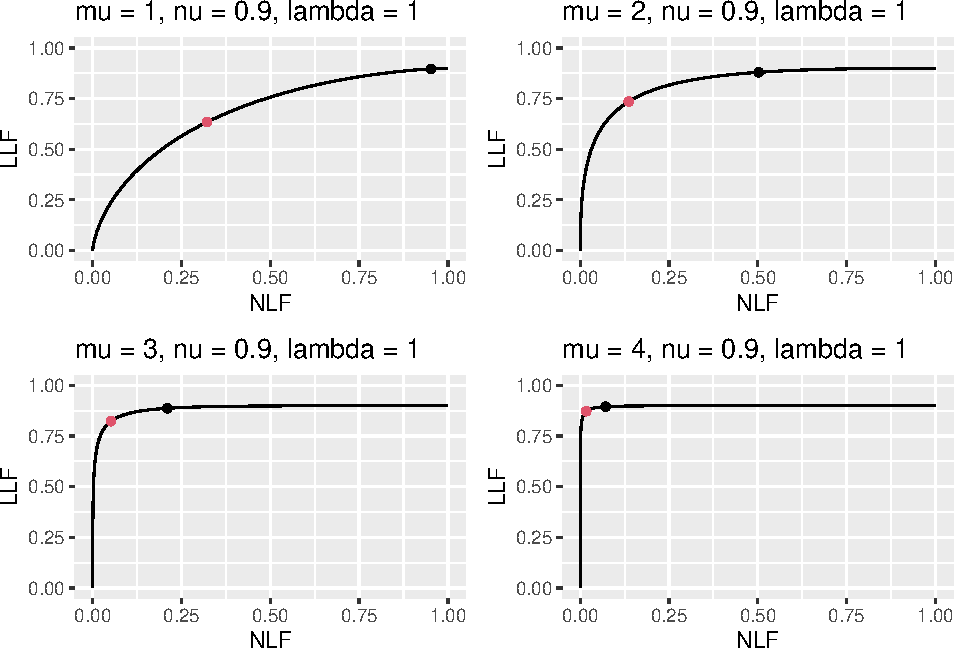
\includegraphics{21-optim-op-point-wafroc_files/figure-latex/optim-op-point-vary-mu-froc-1.pdf}
\caption{\label{fig:optim-op-point-vary-mu-froc}Varying \(\mu\) FROC plots with superimposed operating points. The red dot corresponds to \(\text{wAFROC}_\text{AUC}\) optimization and the black dot to Youden-index optimization. The values of \(\mu\) are: top-left \(\mu = 1\), top-right \(\mu = 2\), bottom-left \(\mu = 3\) and bottom-right \(\mu = 4\).}
\end{figure}

\hypertarget{wafroc-4}{%
\subsubsection{wAFROC}\label{wafroc-4}}

\begin{figure}
\centering
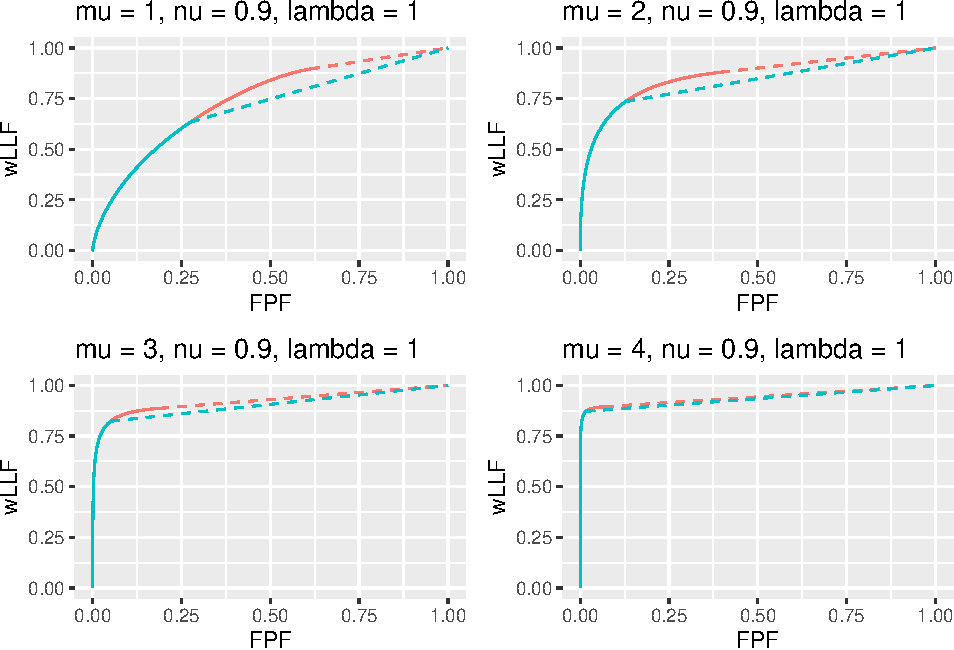
\includegraphics{21-optim-op-point-wafroc_files/figure-latex/optim-op-point-vary-mu-wafroc-1.pdf}
\caption{\label{fig:optim-op-point-vary-mu-wafroc}Varying \(\mu\) wAFROC plots for the two optimization methods with superimposed operating points with superimposed operating points. The color coding is as in previous figures. The values of \(\mu\) are: top-left \(\mu = 1\), top-right \(\mu = 2\), bottom-left \(\mu = 3\) and bottom-right \(\mu = 4\).}
\end{figure}

\hypertarget{roc-4}{%
\subsubsection{ROC}\label{roc-4}}

\begin{figure}
\centering
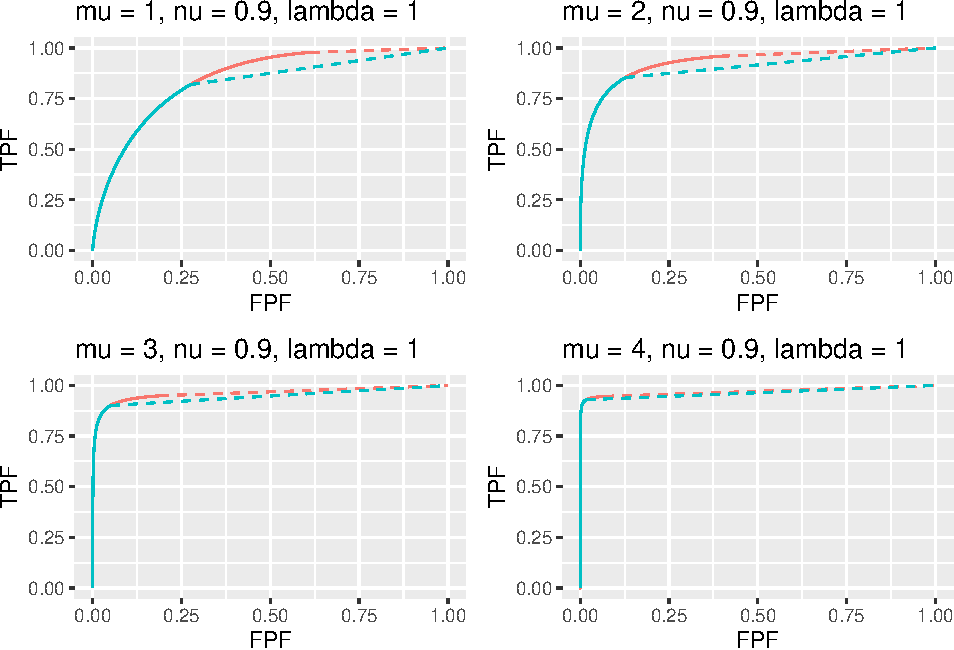
\includegraphics{21-optim-op-point-wafroc_files/figure-latex/optim-op-point-vary-mu-roc-1.pdf}
\caption{\label{fig:optim-op-point-vary-mu-roc}Varying \(\mu\) ROC plots for the two optimization methods with superimposed operating points with superimposed operating points. The color coding is as in previous figures. The values of \(\mu\) are: top-left \(\mu = 1\), top-right \(\mu = 2\), bottom-left \(\mu = 3\) and bottom-right \(\mu = 4\).}
\end{figure}

\hypertarget{optim-op-point-limiting-situations}{%
\subsection{Limiting cases}\label{optim-op-point-limiting-situations}}

\hypertarget{optim-op-point-high-performance-vary-mu}{%
\subsubsection{\texorpdfstring{High performance varying \(\mu\)}{High performance varying \textbackslash mu}}\label{optim-op-point-high-performance-vary-mu}}

\begin{Shaded}
\begin{Highlighting}[]
\NormalTok{muArr }\OtherTok{\textless{}{-}} \FunctionTok{c}\NormalTok{(}\DecValTok{2}\NormalTok{, }\DecValTok{3}\NormalTok{, }\DecValTok{4}\NormalTok{, }\DecValTok{5}\NormalTok{)}
\NormalTok{nuArr }\OtherTok{\textless{}{-}} \FunctionTok{c}\NormalTok{(}\FloatTok{0.9}\NormalTok{)}
\NormalTok{lambdaArr }\OtherTok{\textless{}{-}} \FunctionTok{c}\NormalTok{(}\DecValTok{1}\NormalTok{)}
\end{Highlighting}
\end{Shaded}

\hypertarget{summary-table-4}{%
\paragraph{Summary table}\label{summary-table-4}}

\begin{table}

\caption{\label{tab:optim-op-point-high-performance-vary-mu-table}High performance summary of optimization results for $\lambda = 1$ and $\nu = 0.9$ and varying $\mu$.}
\centering
\fontsize{10}{12}\selectfont
\begin{tabular}[t]{llllll}
\toprule
FOM & $\mu$ & $\zeta_1$ & $\text{wAFROC}_\text{AUC}$ & $\text{ROC}_\text{AUC}$ & $\left( \text{NLF}, \text{LLF}\right)$\\
\midrule
$\text{wAFROC}_\text{AUC}$ & 2 & -0.007 & 0.864 & 0.929 & (0.503, 0.880)\\
 & 3 & 0.808 & 0.922 & 0.961 & (0.210, 0.887)\\
 & 4 & 1.463 & 0.942 & 0.970 & (0.072, 0.895)\\
 & 5 & 2.063 & 0.948 & 0.972 & (0.020, 0.899)\\
Youden-index & 2 & 1.095 & 0.831 & 0.899 & (0.137, 0.735)\\
\addlinespace
 & 3 & 1.629 & 0.903 & 0.945 & (0.052, 0.823)\\
 & 4 & 2.124 & 0.935 & 0.964 & (0.017, 0.873)\\
 & 5 & 2.608 & 0.946 & 0.970 & (0.005, 0.892)\\
\bottomrule
\end{tabular}
\end{table}

\hypertarget{froc-5}{%
\paragraph{FROC}\label{froc-5}}

\begin{figure}
\centering
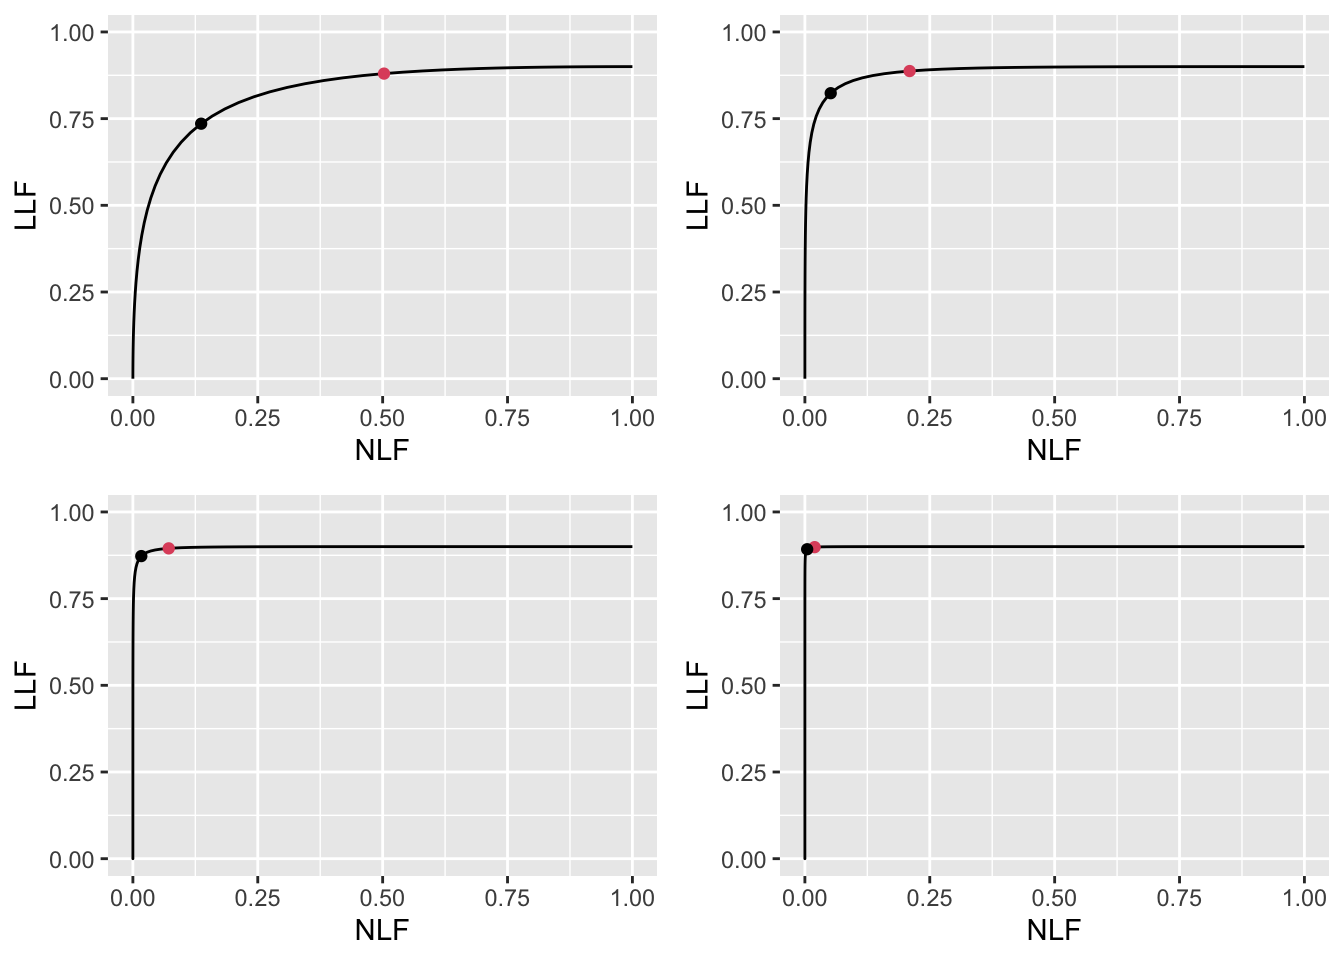
\includegraphics{21-optim-op-point-wafroc_files/figure-latex/optim-op-point-high-performance-vary-mu-froc-1.pdf}
\caption{\label{fig:optim-op-point-high-performance-vary-mu-froc}High performance varying \(\mu\) FROC plots with superimposed operating points. The red dot corresponds to \(\text{wAFROC}_\text{AUC}\) optimization and the black dot to Youden-index optimization. The values of \(\mu\) are: top-left \(\mu = 2\), top-right \(\mu = 3\), bottom-left \(\mu = 4\) and bottom-right \(\mu = 5\).}
\end{figure}

\hypertarget{wafroc-5}{%
\paragraph{wAFROC}\label{wafroc-5}}

\begin{figure}
\centering
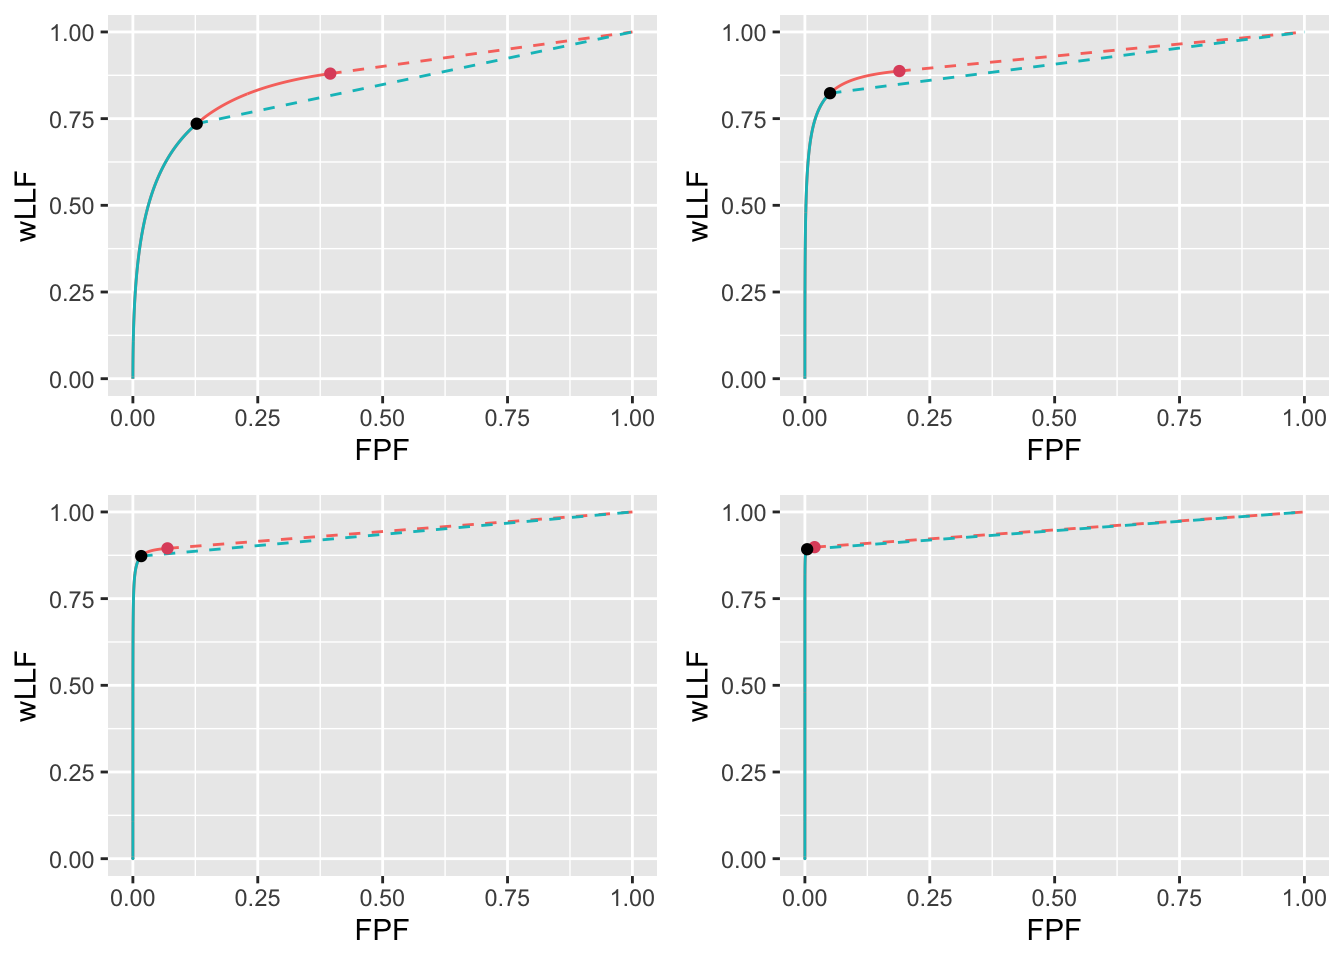
\includegraphics{21-optim-op-point-wafroc_files/figure-latex/optim-op-point-high-performance-vary-mu-wafroc-1.pdf}
\caption{\label{fig:optim-op-point-high-performance-vary-mu-wafroc}High performance varying \(\mu\) wAFROC plots for the two optimization methods with superimposed operating points with superimposed operating points. The color coding is as in previous figures. The values of \(\mu\) are: top-left \(\mu = 2\), top-right \(\mu = 3\), bottom-left \(\mu = 4\) and bottom-right \(\mu = 5\).}
\end{figure}

\hypertarget{roc-5}{%
\paragraph{ROC}\label{roc-5}}

\begin{figure}
\centering
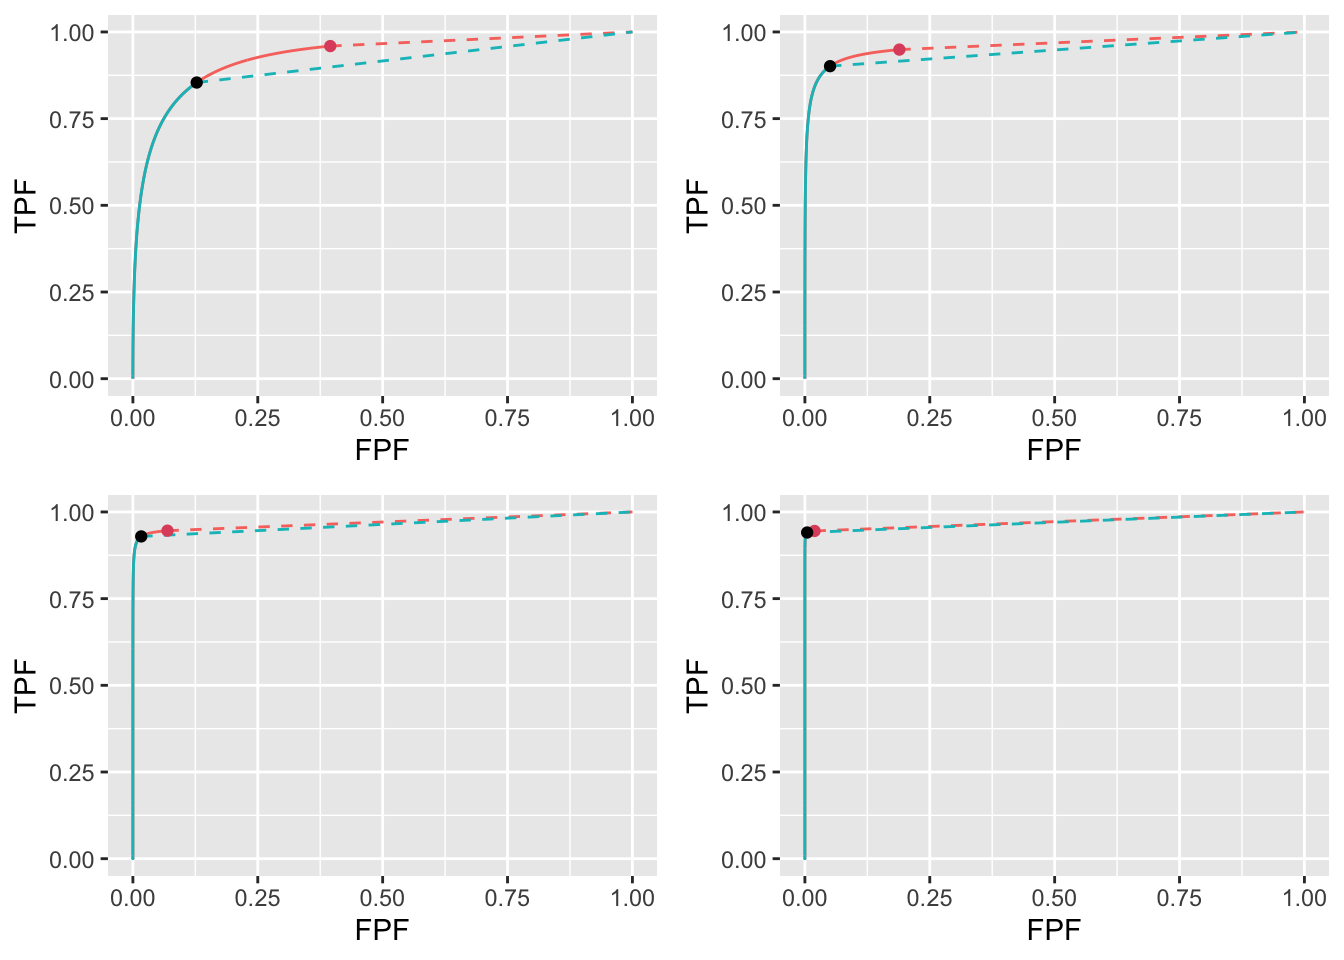
\includegraphics{21-optim-op-point-wafroc_files/figure-latex/optim-op-point-high-performance-vary-mu-roc-1.pdf}
\caption{\label{fig:optim-op-point-high-performance-vary-mu-roc}High performance varying \(\mu\) ROC plots for the two optimization methods with superimposed operating points with superimposed operating points. The color coding is as in previous figures. The values of \(\mu\) are: top-left \(\mu = 2\), top-right \(\mu = 3\), bottom-left \(\mu = 4\) and bottom-right \(\mu = 5\).}
\end{figure}

\hypertarget{optim-op-point-low-performance-vary-mu}{%
\subsubsection{\texorpdfstring{Low performance varying \(\mu\)}{Low performance varying \textbackslash mu}}\label{optim-op-point-low-performance-vary-mu}}

\begin{Shaded}
\begin{Highlighting}[]
\NormalTok{muArr }\OtherTok{\textless{}{-}} \FunctionTok{c}\NormalTok{(}\DecValTok{1}\NormalTok{, }\DecValTok{2}\NormalTok{, }\DecValTok{3}\NormalTok{, }\DecValTok{4}\NormalTok{)}
\NormalTok{nuArr }\OtherTok{\textless{}{-}} \FunctionTok{c}\NormalTok{(}\FloatTok{0.1}\NormalTok{)}
\NormalTok{lambdaArr }\OtherTok{\textless{}{-}} \FunctionTok{c}\NormalTok{(}\DecValTok{10}\NormalTok{)}
\end{Highlighting}
\end{Shaded}

\hypertarget{summary-table-5}{%
\paragraph{Summary table}\label{summary-table-5}}

\begin{table}

\caption{\label{tab:optim-op-point-low-performance-vary-mu-table}Low performance summary of optimization results for $\lambda = 10$ and $nu = 0.1$ and varying $\mu$. Column labeling as in previous tables.}
\centering
\fontsize{10}{12}\selectfont
\begin{tabular}[t]{llllll}
\toprule
FOM & $\mu$ & $\zeta_1$ & $\text{wAFROC}_\text{AUC}$ & $\text{ROC}_\text{AUC}$ & $\left( \text{NLF}, \text{LLF}\right)$\\
\midrule
$\text{wAFROC}_\text{AUC}$ & 1 & 5.000 & 0.500 & 0.500 & (0.000, 0.000)\\
 & 2 & 3.298 & 0.502 & 0.507 & (0.005, 0.010)\\
 & 3 & 3.018 & 0.518 & 0.536 & (0.013, 0.049)\\
 & 4 & 3.130 & 0.536 & 0.559 & (0.009, 0.081)\\
Youden-index & 1 & 1.563 & 0.292 & 0.514 & (0.590, 0.029)\\
\addlinespace
 & 2 & 1.865 & 0.397 & 0.535 & (0.311, 0.055)\\
 & 3 & 2.198 & 0.478 & 0.555 & (0.140, 0.079)\\
 & 4 & 2.564 & 0.523 & 0.567 & (0.052, 0.092)\\
\bottomrule
\end{tabular}
\end{table}

\hypertarget{froc-6}{%
\paragraph{FROC}\label{froc-6}}

\begin{figure}
\centering
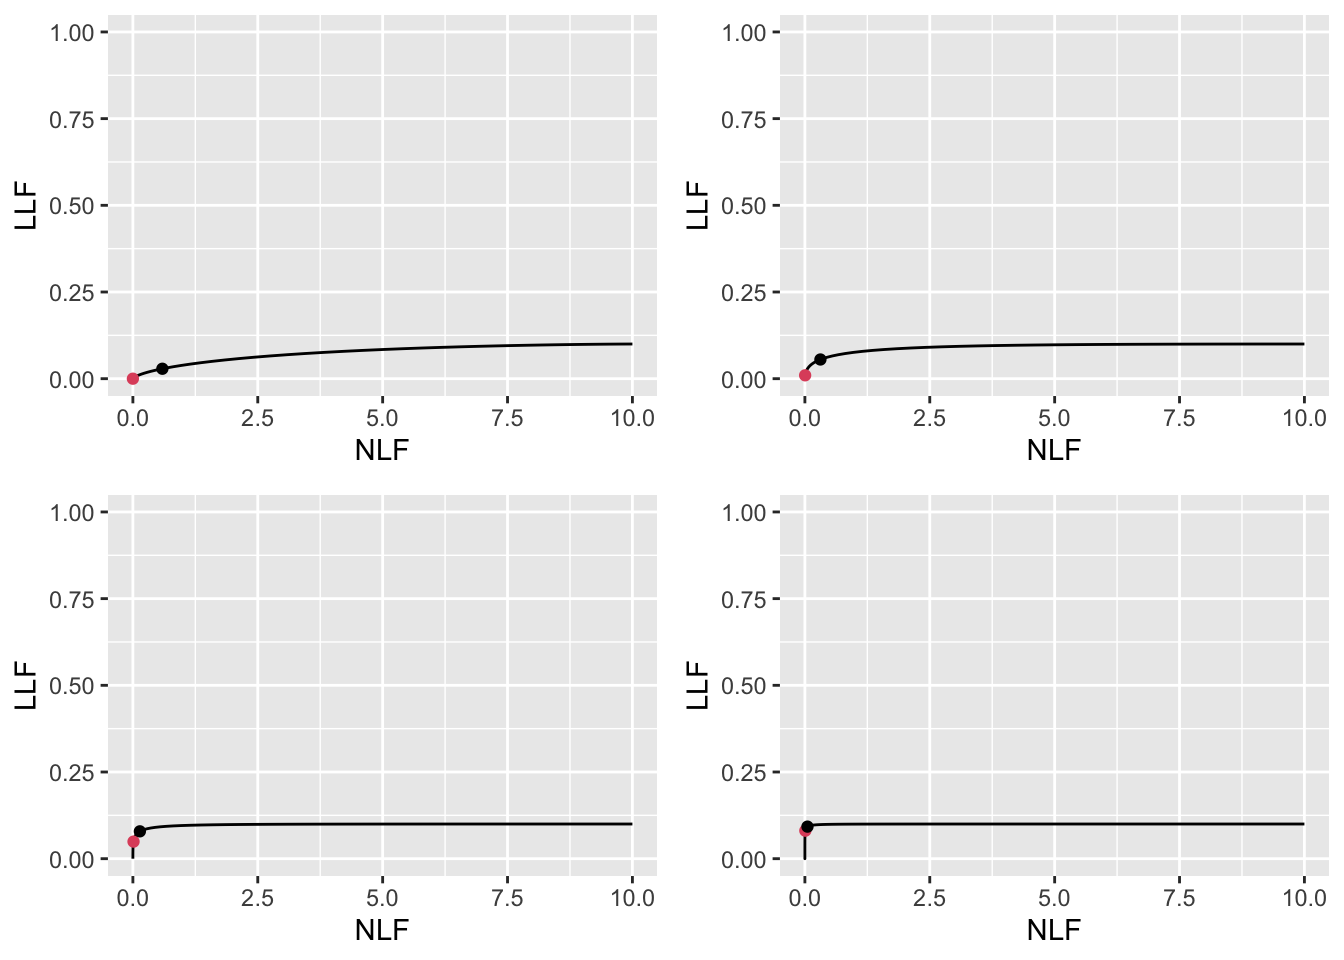
\includegraphics{21-optim-op-point-wafroc_files/figure-latex/optim-op-point-low-performance-vary-mu-1.pdf}
\caption{\label{fig:optim-op-point-low-performance-vary-mu}Low performance varying \(\mu\) FROC plots with superimposed operating points. The red dot corresponds to \(\text{wAFROC}_\text{AUC}\) optimization and the black dot to Youden-index optimization. The values of \(\mu\) are: top-left \(\mu = 1\), top-right \(\mu = 2\), bottom-left \(\mu = 3\) and bottom-right \(\mu = 4\).}
\end{figure}

\hypertarget{wafroc-6}{%
\paragraph{wAFROC}\label{wafroc-6}}

\begin{figure}
\centering
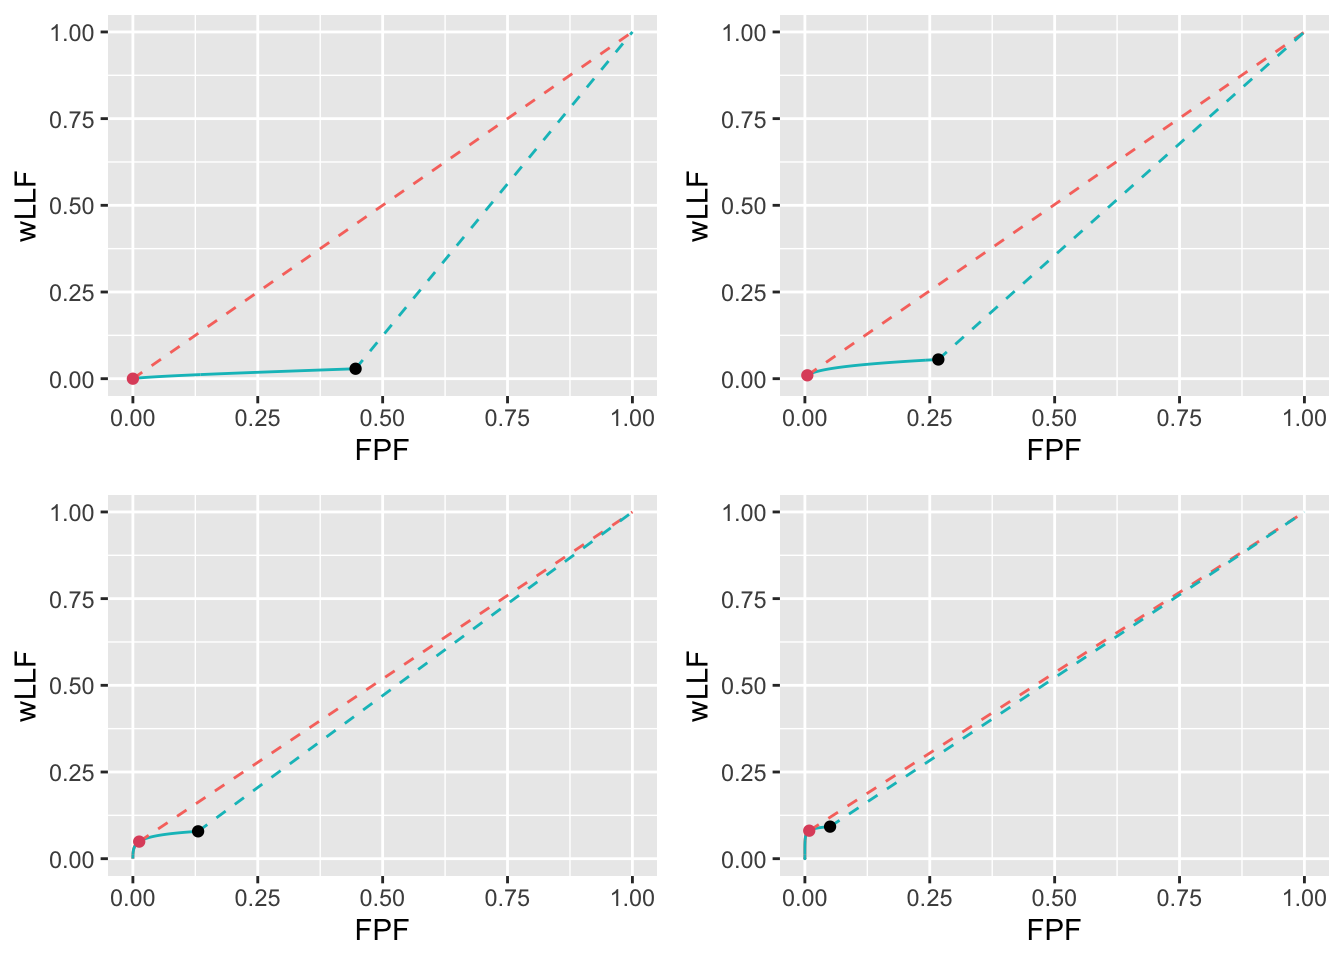
\includegraphics{21-optim-op-point-wafroc_files/figure-latex/optim-op-point-low-performance-vary-mu-wafroc-1.pdf}
\caption{\label{fig:optim-op-point-low-performance-vary-mu-wafroc}Low performance varying \(\mu\) wAFROC plots for the two optimization methods with superimposed operating points with superimposed operating points. The color coding is as in previous figures. The values of \(\mu\) are: top-left \(\mu = 1\), top-right \(\mu = 2\), bottom-left \(\mu = 3\) and bottom-right \(\mu = 4\).}
\end{figure}

\hypertarget{roc-6}{%
\paragraph{ROC}\label{roc-6}}

\begin{figure}
\centering
\includegraphics{21-optim-op-point-wafroc_files/figure-latex/optim-op-point-low-performance-vary-mu-roc-1.pdf}
\caption{\label{fig:optim-op-point-low-performance-vary-mu-roc}Low performance varying \(\mu\) ROC plots for the two optimization methods with superimposed operating points with superimposed operating points. The color coding is as in previous figures. The values of \(\mu\) are: top-left \(\mu = 1\), top-right \(\mu = 2\), bottom-left \(\mu = 3\) and bottom-right \(\mu = 4\).}
\end{figure}

\hypertarget{optim-op-point-high-performance-vary-lambda}{%
\subsubsection{\texorpdfstring{High performance varying \(\lambda\)}{High performance varying \textbackslash lambda}}\label{optim-op-point-high-performance-vary-lambda}}

\begin{Shaded}
\begin{Highlighting}[]
\NormalTok{muArr }\OtherTok{\textless{}{-}} \FunctionTok{c}\NormalTok{(}\DecValTok{4}\NormalTok{)}
\NormalTok{nuArr }\OtherTok{\textless{}{-}} \FunctionTok{c}\NormalTok{(}\FloatTok{0.9}\NormalTok{)}
\NormalTok{lambdaArr }\OtherTok{\textless{}{-}} \FunctionTok{c}\NormalTok{(}\DecValTok{1}\NormalTok{,}\DecValTok{2}\NormalTok{,}\DecValTok{5}\NormalTok{,}\DecValTok{10}\NormalTok{)}
\end{Highlighting}
\end{Shaded}

\hypertarget{summary-table-6}{%
\paragraph{Summary table}\label{summary-table-6}}

\begin{table}

\caption{\label{tab:optim-op-point-high-performance-vary-lambda-table}Results for $\mu = 4$, $nu = 0.9$ and varying $\lambda$. Column labeling as in previous tables.}
\centering
\fontsize{10}{12}\selectfont
\begin{tabular}[t]{llllll}
\toprule
FOM & $\lambda$ & $\zeta_1$ & $\text{wAFROC}_\text{AUC}$ & $\text{ROC}_\text{AUC}$ & $\left( \text{NLF}, \text{LLF}\right)$\\
\midrule
$\text{wAFROC}_\text{AUC}$ & 1 & 1.463 & 0.942 & 0.970 & (0.072, 0.895)\\
 & 2 & 1.644 & 0.938 & 0.968 & (0.100, 0.892)\\
 & 5 & 1.889 & 0.930 & 0.965 & (0.147, 0.884)\\
 & 10 & 2.082 & 0.920 & 0.960 & (0.187, 0.875)\\
Youden-index & 1 & 2.124 & 0.935 & 0.964 & (0.017, 0.873)\\
\addlinespace
 & 2 & 2.291 & 0.928 & 0.960 & (0.022, 0.861)\\
 & 5 & 2.508 & 0.915 & 0.952 & (0.030, 0.839)\\
 & 10 & 2.669 & 0.903 & 0.944 & (0.038, 0.818)\\
\bottomrule
\end{tabular}
\end{table}

\hypertarget{froc-7}{%
\paragraph{FROC}\label{froc-7}}

\begin{figure}
\centering
\includegraphics{21-optim-op-point-wafroc_files/figure-latex/optim-op-point-high-performance-vary-lambda-froc-1.pdf}
\caption{\label{fig:optim-op-point-high-performance-vary-lambda-froc}High performance varying \(\lambda\) FROC plots with superimposed operating points. The red dot corresponds to \(\text{wAFROC}_\text{AUC}\) optimization and the black dot to Youden-index optimization. The values of \(\lambda\) are: top-left \(\lambda = 1\), top-right \(\lambda = 2\), bottom-left \(\lambda = 5\) and bottom-right \(\lambda = 10\).}
\end{figure}

\hypertarget{wafroc-7}{%
\paragraph{wAFROC}\label{wafroc-7}}

\begin{figure}
\centering
\includegraphics{21-optim-op-point-wafroc_files/figure-latex/optim-op-point-high-performance-vary-lambda-wafroc-1.pdf}
\caption{\label{fig:optim-op-point-high-performance-vary-lambda-wafroc}High performance varying \(\lambda\) wAFROC plots for the two optimization methods with superimposed operating points. The color coding is as in previous figures. The values of \(\lambda\) are: top-left \(\lambda = 1\), top-right \(\lambda = 2\), bottom-left \(\lambda = 5\) and bottom-right \(\lambda = 10\).}
\end{figure}

\hypertarget{roc-7}{%
\paragraph{ROC}\label{roc-7}}

\begin{figure}
\centering
\includegraphics{21-optim-op-point-wafroc_files/figure-latex/optim-op-point-high-performance-vary-lambda-roc-1.pdf}
\caption{\label{fig:optim-op-point-high-performance-vary-lambda-roc}High performance varying \(\lambda\) ROC plots for the two optimization methods with superimposed operating points. The color coding is as in previous figures. The values of \(\lambda\) are: top-left \(\lambda = 1\), top-right \(\lambda = 2\), bottom-left \(\lambda = 5\) and bottom-right \(\lambda = 10\).}
\end{figure}

\hypertarget{optim-op-point-low-performance-vary-lambda}{%
\subsubsection{\texorpdfstring{Low performance varying \(\lambda\)}{Low performance varying \textbackslash lambda}}\label{optim-op-point-low-performance-vary-lambda}}

\begin{Shaded}
\begin{Highlighting}[]
\NormalTok{muArr }\OtherTok{\textless{}{-}} \FunctionTok{c}\NormalTok{(}\DecValTok{1}\NormalTok{)}
\NormalTok{nuArr }\OtherTok{\textless{}{-}} \FunctionTok{c}\NormalTok{(}\FloatTok{0.2}\NormalTok{)}
\NormalTok{lambdaArr }\OtherTok{\textless{}{-}} \FunctionTok{c}\NormalTok{(}\DecValTok{1}\NormalTok{, }\DecValTok{2}\NormalTok{, }\DecValTok{5}\NormalTok{, }\DecValTok{10}\NormalTok{)}
\end{Highlighting}
\end{Shaded}

\hypertarget{summary-table-7}{%
\paragraph{Summary table}\label{summary-table-7}}

\begin{table}

\caption{\label{tab:optim-op-point-low-performance-vary-lambda-table}Results for $\mu = 1$, $\nu = 0.2$ and varying $\lambda$. Column labeling as in previous tables.}
\centering
\fontsize{10}{12}\selectfont
\begin{tabular}[t]{llllll}
\toprule
FOM & $\lambda$ & $\zeta_1$ & $\text{wAFROC}_\text{AUC}$ & $\text{ROC}_\text{AUC}$ & $\left( \text{NLF}, \text{LLF}\right)$\\
\midrule
$\text{wAFROC}_\text{AUC}$ & 1 & 2.081 & 0.505 & 0.520 & (0.019, 0.028)\\
 & 2 & 2.795 & 0.501 & 0.505 & (0.005, 0.007)\\
 & 5 & 3.718 & 0.500 & 0.500 & (0.001, 0.001)\\
 & 10 & 4.412 & 0.500 & 0.500 & (0.000, 0.000)\\
Youden-index & 1 & 0.284 & 0.423 & 0.587 & (0.388, 0.153)\\
\addlinespace
 & 2 & 0.734 & 0.380 & 0.566 & (0.463, 0.121)\\
 & 5 & 1.237 & 0.335 & 0.542 & (0.540, 0.081)\\
 & 10 & 1.568 & 0.309 & 0.528 & (0.585, 0.057)\\
\bottomrule
\end{tabular}
\end{table}

\hypertarget{froc-8}{%
\paragraph{FROC}\label{froc-8}}

\begin{figure}
\centering
\includegraphics{21-optim-op-point-wafroc_files/figure-latex/optim-op-point-low-performance-vary-lambda-froc-1.pdf}
\caption{\label{fig:optim-op-point-low-performance-vary-lambda-froc}Low performance varying \(\lambda\) FROC plots with superimposed operating points. The red dot corresponds to \(\text{wAFROC}_\text{AUC}\) optimization and the black dot to Youden-index optimization. The values of \(\lambda\) are: top-left \(\lambda = 1\), top-right \(\lambda = 2\), bottom-left \(\lambda = 5\) and bottom-right \(\lambda = 10\).}
\end{figure}

\hypertarget{wafroc-8}{%
\paragraph{wAFROC}\label{wafroc-8}}

\begin{figure}
\centering
\includegraphics{21-optim-op-point-wafroc_files/figure-latex/optim-op-point-low-performance-vary-lambda-wafroc-1.pdf}
\caption{\label{fig:optim-op-point-low-performance-vary-lambda-wafroc}Low performance varying \(\lambda\) wAFROC plots for the two optimization methods with superimposed operating points. The color coding is as in previous figures. The values of \(\lambda\) are: top-left \(\lambda = 1\), top-right \(\lambda = 2\), bottom-left \(\lambda = 5\) and bottom-right \(\lambda = 10\).}
\end{figure}

\hypertarget{roc-8}{%
\paragraph{ROC}\label{roc-8}}

\begin{figure}
\centering
\includegraphics{21-optim-op-point-wafroc_files/figure-latex/optim-op-point-low-performance-vary-lambda-roc-1.pdf}
\caption{\label{fig:optim-op-point-low-performance-vary-lambda-roc}Low performance varying \(\lambda\) ROC plots for the two optimization methods with superimposed operating points. The color coding is as in previous figures. The values of \(\lambda\) are: top-left \(\lambda = 1\), top-right \(\lambda = 2\), bottom-left \(\lambda = 5\) and bottom-right \(\lambda = 10\).}
\end{figure}

\hypertarget{optim-op-point-high-performance-vary-nu}{%
\subsubsection{\texorpdfstring{High performance varying \(\nu\)}{High performance varying \textbackslash nu}}\label{optim-op-point-high-performance-vary-nu}}

\begin{Shaded}
\begin{Highlighting}[]
\NormalTok{muArr }\OtherTok{\textless{}{-}} \FunctionTok{c}\NormalTok{(}\DecValTok{4}\NormalTok{)}
\NormalTok{lambdaArr }\OtherTok{\textless{}{-}} \FunctionTok{c}\NormalTok{(}\DecValTok{1}\NormalTok{)}
\NormalTok{nuArr }\OtherTok{\textless{}{-}} \FunctionTok{c}\NormalTok{(}\FloatTok{0.6}\NormalTok{, }\FloatTok{0.7}\NormalTok{, }\FloatTok{0.8}\NormalTok{, }\FloatTok{0.9}\NormalTok{)}
\end{Highlighting}
\end{Shaded}

\hypertarget{summary-table-8}{%
\paragraph{Summary table}\label{summary-table-8}}

\begin{table}

\caption{\label{tab:optim-op-point-high-performance-vary-nu-table}Results for $\mu = 4$, $\lambda = 1$ and varying $\nu$. Column labeling as in previous tables.}
\centering
\fontsize{10}{12}\selectfont
\begin{tabular}[t]{llllll}
\toprule
FOM & $\nu$ & $\zeta_1$ & $\text{wAFROC}_\text{AUC}$ & $\text{ROC}_\text{AUC}$ & $\left( \text{NLF}, \text{LLF}\right)$\\
\midrule
$\text{wAFROC}_\text{AUC}$ & 0.6 & 1.905 & 0.788 & 0.855 & (0.028, 0.589)\\
 & 0.7 & 1.796 & 0.839 & 0.898 & (0.036, 0.690)\\
 & 0.8 & 1.663 & 0.890 & 0.936 & (0.048, 0.792)\\
 & 0.9 & 1.463 & 0.942 & 0.970 & (0.072, 0.895)\\
Youden-index & 0.6 & 2.063 & 0.788 & 0.852 & (0.020, 0.584)\\
\addlinespace
 & 0.7 & 2.080 & 0.837 & 0.894 & (0.019, 0.681)\\
 & 0.8 & 2.100 & 0.886 & 0.931 & (0.018, 0.777)\\
 & 0.9 & 2.124 & 0.935 & 0.964 & (0.017, 0.873)\\
\bottomrule
\end{tabular}
\end{table}

\hypertarget{froc-9}{%
\paragraph{FROC}\label{froc-9}}

\begin{figure}
\centering
\includegraphics{21-optim-op-point-wafroc_files/figure-latex/optim-op-point-high-performance-vary-nu-froc-1.pdf}
\caption{\label{fig:optim-op-point-high-performance-vary-nu-froc}High performance varying \(\nu\) FROC plots with superimposed operating points. The red dot corresponds to \(\text{wAFROC}_\text{AUC}\) optimization and the black dot to Youden-index optimization. The values of \(\nu\) are: top-left \(\nu = 0.6\), top-right \(\nu = 0.7\), bottom-left \(\nu = 0.8\) and bottom-right \(\nu = 0.9\).}
\end{figure}

\hypertarget{wafroc-9}{%
\paragraph{wAFROC}\label{wafroc-9}}

\begin{figure}
\centering
\includegraphics{21-optim-op-point-wafroc_files/figure-latex/optim-op-point-high-performance-vary-nu-wafroc-1.pdf}
\caption{\label{fig:optim-op-point-high-performance-vary-nu-wafroc}High performance varying \(\nu\) wAFROC plots for the two optimization methods with superimposed operating points. The color coding is as in previous figures. The values of \(\nu\) are: top-left \(\nu = 0.6\), top-right \(\nu = 0.7\), bottom-left \(\nu = 0.8\) and bottom-right \(\nu = 0.9\).}
\end{figure}

\hypertarget{roc-9}{%
\paragraph{ROC}\label{roc-9}}

\begin{figure}
\centering
\includegraphics{21-optim-op-point-wafroc_files/figure-latex/optim-op-point-high-performance-vary-nu-roc-1.pdf}
\caption{\label{fig:optim-op-point-high-performance-vary-nu-roc}High performance varying \(\nu\) ROC plots for the two optimization methods with superimposed operating points. The color coding is as in previous figures. The values of \(\nu\) are: top-left \(\nu = 0.6\), top-right \(\nu = 0.7\), bottom-left \(\nu = 0.8\) and bottom-right \(\nu = 0.9\).}
\end{figure}

\hypertarget{optim-op-point-low-performance-vary-nu}{%
\subsubsection{\texorpdfstring{Low performance varying \(\nu\)}{Low performance varying \textbackslash nu}}\label{optim-op-point-low-performance-vary-nu}}

\begin{Shaded}
\begin{Highlighting}[]
\NormalTok{muArr }\OtherTok{\textless{}{-}} \FunctionTok{c}\NormalTok{(}\DecValTok{1}\NormalTok{)}
\NormalTok{lambdaArr }\OtherTok{\textless{}{-}} \FunctionTok{c}\NormalTok{(}\DecValTok{10}\NormalTok{)}
\NormalTok{nuArr }\OtherTok{\textless{}{-}} \FunctionTok{c}\NormalTok{(}\FloatTok{0.1}\NormalTok{, }\FloatTok{0.2}\NormalTok{, }\FloatTok{0.3}\NormalTok{, }\FloatTok{0.4}\NormalTok{)}
\end{Highlighting}
\end{Shaded}

\hypertarget{summary-table-9}{%
\paragraph{Summary table}\label{summary-table-9}}

\begin{table}

\caption{\label{tab:optim-op-point-low-performance-vary-nu-table}Results for $\mu = 1$, $\lambda = 10$ and varying $\nu$. Column labeling as in previous tables.}
\centering
\fontsize{10}{12}\selectfont
\begin{tabular}[t]{llllll}
\toprule
FOM & $\nu$ & $\zeta_1$ & $\text{wAFROC}_\text{AUC}$ & $\text{ROC}_\text{AUC}$ & $\left( \text{NLF}, \text{LLF}\right)$\\
\midrule
$\text{wAFROC}_\text{AUC}$ & 0.1 & 5.000 & 0.500 & 0.500 & (0.000, 0.000)\\
 & 0.2 & 4.412 & 0.500 & 0.500 & (0.000, 0.000)\\
 & 0.3 & 4.006 & 0.500 & 0.500 & (0.000, 0.000)\\
 & 0.4 & 3.718 & 0.500 & 0.501 & (0.001, 0.001)\\
Youden-index & 0.1 & 1.563 & 0.292 & 0.514 & (0.590, 0.029)\\
\addlinespace
 & 0.2 & 1.568 & 0.309 & 0.528 & (0.585, 0.057)\\
 & 0.3 & 1.572 & 0.325 & 0.542 & (0.580, 0.085)\\
 & 0.4 & 1.577 & 0.342 & 0.556 & (0.574, 0.113)\\
\bottomrule
\end{tabular}
\end{table}

\hypertarget{froc-10}{%
\paragraph{FROC}\label{froc-10}}

\begin{figure}
\centering
\includegraphics{21-optim-op-point-wafroc_files/figure-latex/optim-op-point-low-performance-vary-nu-froc-1.pdf}
\caption{\label{fig:optim-op-point-low-performance-vary-nu-froc}Low performance varying \(\nu\) FROC plots with superimposed operating points. The red dot corresponds to \(\text{wAFROC}_\text{AUC}\) optimization and the black dot to Youden-index optimization. The values of \(\nu\) are: top-left \(\nu = 0.1\), top-right \(\nu = 0.2\), bottom-left \(\nu = 0.3\) and bottom-right \(\nu = 0.4\).}
\end{figure}

\hypertarget{wafroc-10}{%
\paragraph{wAFROC}\label{wafroc-10}}

\begin{figure}
\centering
\includegraphics{21-optim-op-point-wafroc_files/figure-latex/optim-op-point-low-performance-vary-nu-wafroc-1.pdf}
\caption{\label{fig:optim-op-point-low-performance-vary-nu-wafroc}Low performance varying \(\nu\) wAFROC plots for the two optimization methods with superimposed operating points. The color coding is as in previous figures. The values of \(\nu\) are: top-left \(\nu = 0.1\), top-right \(\nu = 0.2\), bottom-left \(\nu = 0.3\) and bottom-right \(\nu = 0.4\).}
\end{figure}

\hypertarget{roc-10}{%
\paragraph{ROC}\label{roc-10}}

\begin{figure}
\centering
\includegraphics{21-optim-op-point-wafroc_files/figure-latex/optim-op-point-low-performance-vary-nu-roc-1.pdf}
\caption{\label{fig:optim-op-point-low-performance-vary-nu-roc}Low performance varying \(\nu\) ROC plots for the two optimization methods with superimposed operating points. The color coding is as in previous figures. The values of \(\nu\) are: top-left \(\nu = 0.1\), top-right \(\nu = 0.2\), bottom-left \(\nu = 0.3\) and bottom-right \(\nu = 0.4\).}
\end{figure}

\hypertarget{analyze-diseased-only-dataset}{%
\chapter{Analyzing a dataset with only diseased cases}\label{analyze-diseased-only-dataset}}

\hypertarget{analyze-diseased-only-dataset-how-much-finished}{%
\section{TBA How much finished}\label{analyze-diseased-only-dataset-how-much-finished}}

0\%

\hypertarget{analyze-diseased-only-dataset-methods}{%
\section{The problem}\label{analyze-diseased-only-dataset-methods}}

How to analyze \(K_1 = 0\) datasets.

ROC-like plot of TPF vs.~FPF1 is possible, see Section \ref{empirical-definition-empirical-auc-afroc1}. Can create a ROC-like dataset with equal number of ``non-diseased'' and diseased cases (the ratings of the non-diseased cases are the FP ratings on diseased cases). Fit RSM to this dataset. Proceed as before. Key assumption being violated: the FP ratings on diseased cases are independent of the TP ratings on same cases. However, without this assumption one cannot estimate RSM parameters. Need \texttt{RJafroc} function to handle this special case: \texttt{FitRsmRoc1}? No! Just need function to create a ``ROC'' dataset from one that only has diseased cases. e.g., \texttt{DfNoNormalsDataset}?

\hypertarget{analyze-diseased-only-dataset-step-1}{%
\subsection{Step 1: Create a test (diseased cases only) dataset}\label{analyze-diseased-only-dataset-step-1}}

Save TONY dataset to \texttt{dsTony}. Create copy \texttt{dsNoNormals}. Remove all normal cases from it.

\begin{Shaded}
\begin{Highlighting}[]
\NormalTok{dsTony }\OtherTok{\textless{}{-}}\NormalTok{ RJafroc}\SpecialCharTok{::}\NormalTok{dataset01 }\CommentTok{\# TONY dataset}
\NormalTok{K2 }\OtherTok{\textless{}{-}} \FunctionTok{length}\NormalTok{(dsTony}\SpecialCharTok{$}\NormalTok{lesions}\SpecialCharTok{$}\NormalTok{perCase)}
\NormalTok{K1 }\OtherTok{\textless{}{-}} \FunctionTok{length}\NormalTok{(dsTony}\SpecialCharTok{$}\NormalTok{ratings}\SpecialCharTok{$}\NormalTok{NL[}\DecValTok{1}\NormalTok{,}\DecValTok{1}\NormalTok{,,}\DecValTok{1}\NormalTok{]) }\SpecialCharTok{{-}}\NormalTok{ K2}
\NormalTok{dsNoNormals }\OtherTok{\textless{}{-}}\NormalTok{ dsTony}
\CommentTok{\# Remove all normal cases}
\NormalTok{dsNoNormals}\SpecialCharTok{$}\NormalTok{ratings}\SpecialCharTok{$}\NormalTok{NL }\OtherTok{\textless{}{-}}\NormalTok{ dsNoNormals}\SpecialCharTok{$}\NormalTok{ratings}\SpecialCharTok{$}\NormalTok{NL[,,}\SpecialCharTok{{-}}\NormalTok{(}\DecValTok{1}\SpecialCharTok{:}\NormalTok{K1),] }
\CommentTok{\# And fix truthTableStr}
\NormalTok{dsNoNormals}\SpecialCharTok{$}\NormalTok{descriptions}\SpecialCharTok{$}\NormalTok{truthTableStr }\OtherTok{\textless{}{-}} 
\NormalTok{  dsNoNormals}\SpecialCharTok{$}\NormalTok{descriptions}\SpecialCharTok{$}\NormalTok{truthTableStr[,,}\SpecialCharTok{{-}}\NormalTok{(}\DecValTok{1}\SpecialCharTok{:}\NormalTok{K1),]}
\NormalTok{RJafroc}\SpecialCharTok{::}\FunctionTok{UtilFigureOfMerit}\NormalTok{(dsTony,}\AttributeTok{FOM =} \StringTok{"wAFROC"}\NormalTok{)}
\CommentTok{\#\textgreater{}            rdr1      rdr2      rdr3      rdr4      rdr5}
\CommentTok{\#\textgreater{} trtBT 0.7602704 0.8406191 0.8171524 0.8153090 0.8278324}
\CommentTok{\#\textgreater{} trtDM 0.6425854 0.7049977 0.7518434 0.7724426 0.6836962}
\CommentTok{\#RJafroc::UtilFigureOfMerit(dsNoNormals,FOM = "wAFROC") \#this will generate an error}
\NormalTok{RJafroc}\SpecialCharTok{::}\FunctionTok{UtilFigureOfMerit}\NormalTok{(dsTony,}\AttributeTok{FOM =} \StringTok{"wAFROC1"}\NormalTok{)}
\CommentTok{\#\textgreater{}            rdr1      rdr2      rdr3      rdr4      rdr5}
\CommentTok{\#\textgreater{} trtBT 0.8079866 0.8696629 0.8747798 0.8517613 0.8563468}
\CommentTok{\#\textgreater{} trtDM 0.7277103 0.7781506 0.8225630 0.7968418 0.7496963}
\NormalTok{RJafroc}\SpecialCharTok{::}\FunctionTok{UtilFigureOfMerit}\NormalTok{(dsNoNormals,}\AttributeTok{FOM =} \StringTok{"wAFROC1"}\NormalTok{)}
\CommentTok{\#\textgreater{}            rdr1      rdr2      rdr3      rdr4      rdr5}
\CommentTok{\#\textgreater{} trtBT 0.8594559 0.9009910 0.9369398 0.8910807 0.8871039}
\CommentTok{\#\textgreater{} trtDM 0.8195304 0.8570572 0.8988448 0.8231600 0.8208875}
\NormalTok{st }\OtherTok{\textless{}{-}} \FunctionTok{StSignificanceTesting}\NormalTok{(dsTony,}\AttributeTok{FOM =} \StringTok{"wAFROC"}\NormalTok{)}
\NormalTok{st1 }\OtherTok{\textless{}{-}} \FunctionTok{StSignificanceTesting}\NormalTok{(dsNoNormals,}\AttributeTok{FOM =} \StringTok{"wAFROC1"}\NormalTok{)}
\NormalTok{st}\SpecialCharTok{$}\NormalTok{RRRC}
\CommentTok{\#\textgreater{} $FTests}
\CommentTok{\#\textgreater{}                  DF         MS     FStat            p}
\CommentTok{\#\textgreater{} Treatment  1.000000 4.72951648 10.298825 0.0036685784}
\CommentTok{\#\textgreater{} Error     24.702758 0.45922873        NA           NA}
\CommentTok{\#\textgreater{} }
\CommentTok{\#\textgreater{} $ciDiffTrt}
\CommentTok{\#\textgreater{}              Estimate      StdErr        DF         t        PrGTt     CILower}
\CommentTok{\#\textgreater{} trtBT{-}trtDM 0.1011236 0.031510744 24.702758 3.2091783 0.0036685784 0.036186385}
\CommentTok{\#\textgreater{}                CIUpper}
\CommentTok{\#\textgreater{} trtBT{-}trtDM 0.16606081}
\CommentTok{\#\textgreater{} }
\CommentTok{\#\textgreater{} $ciAvgRdrEachTrt}
\CommentTok{\#\textgreater{}         Estimate      StdErr        DF    CILower    CIUpper}
\CommentTok{\#\textgreater{} trtBT 0.81223666 0.026984337 59.281486 0.75824649 0.86622683}
\CommentTok{\#\textgreater{} trtDM 0.71111306 0.033910209 17.789298 0.63980982 0.78241630}
\NormalTok{st1}\SpecialCharTok{$}\NormalTok{RRRC}
\CommentTok{\#\textgreater{} $FTests}
\CommentTok{\#\textgreater{}                  DF          MS     FStat            p}
\CommentTok{\#\textgreater{} Treatment   1.00000 0.583686978 7.9579613 0.0051936318}
\CommentTok{\#\textgreater{} Error     236.88206 0.073346295        NA           NA}
\CommentTok{\#\textgreater{} }
\CommentTok{\#\textgreater{} $ciDiffTrt}
\CommentTok{\#\textgreater{}                Estimate      StdErr        DF         t        PrGTt}
\CommentTok{\#\textgreater{} trtBT{-}trtDM 0.051218281 0.018156163 236.88206 2.8209859 0.0051936318}
\CommentTok{\#\textgreater{}                 CILower    CIUpper}
\CommentTok{\#\textgreater{} trtBT{-}trtDM 0.015450111 0.08698645}
\CommentTok{\#\textgreater{} }
\CommentTok{\#\textgreater{} $ciAvgRdrEachTrt}
\CommentTok{\#\textgreater{}         Estimate      StdErr        DF    CILower    CIUpper}
\CommentTok{\#\textgreater{} trtBT 0.89511425 0.019745498 24.733020 0.85442537 0.93580314}
\CommentTok{\#\textgreater{} trtDM 0.84389597 0.024970629 27.621445 0.79271436 0.89507759}
\end{Highlighting}
\end{Shaded}

\begin{itemize}
\item
  \texttt{dsNoNormals} is the dataset with no non-diseased cases.
\item
  \texttt{st} contains the results of significance testing using the wAFROC-AUC figure of merit for the full dataset.
\item
  \texttt{st1} contains the results of significance testing using the wAFROC1-AUC figure of merit for the dataset with no non-diseased cases.
\end{itemize}

  \bibliography{packages.bib,myRefs.bib}

\end{document}
